% This is an automatically generated file, do not modify manually!
% This book is published using Seaside, Magritte and the Pier book publishing engine.
% 23 June 2012 3:52:23 pm

\documentclass[a4paper,10pt,twoside]{book}
\usepackage[
	papersize={6.13in,9.21in},
	hmargin={.75in,.75in},
	vmargin={.75in,1in},
	ignoreheadfoot
]{geometry}

% packages
\usepackage{tikz}
\usepackage{color}
\usepackage{xcolor}
\usepackage{xspace}
\usepackage{ifthen}
\usepackage{amsbsy}
\usepackage{amssymb}
\usepackage{tabularx}
\usepackage{verbatim}
\usepackage{needspace}
\usepackage{microtype}

% english
\usepackage[english]{babel}
\usepackage[parfill]{parskip}
\usepackage[normalem]{ulem}

% fonts
\usepackage{lmodern}
\usepackage{palatino}
\usepackage[T1]{fontenc}

% references
\usepackage{hyperref}
\usepackage[all]{hypcap}
\setcounter{tocdepth}{2}
\hypersetup{
	colorlinks=true,
	linkcolor=black,
	anchorcolor=black,
	citecolor=black,
	filecolor=black,
	pagecolor=black,
	urlcolor=black,
	plainpages=black,
	bookmarksopen=true,
	bookmarksopenlevel=2}

% boxes
\newsavebox{\StandoutBox}

\definecolor{noteBackground}{HTML}{EBEBEB}
\definecolor{noteForeground}{HTML}{777777}
\newenvironment{note}%
	{\begin{lrbox}{\StandoutBox}%
	 \begin{minipage}{0.97\textwidth}}
	{\end{minipage}%
	 \end{lrbox}%
	 \begin{center}
		\begin{tikzpicture}
			\node [fill=noteBackground, rectangle, rounded corners, inner sep=5pt] (box)
				{\usebox{\StandoutBox}};
			\node [text=noteForeground, anchor=south west] at (box.north west)
				{\textbf{Note}};
		\end{tikzpicture}
	 \end{center}}

\definecolor{advancedBackground}{HTML}{D9E6EE}
\definecolor{advancedForeground}{HTML}{01598E}
\newenvironment{advanced}%
	{\begin{lrbox}{\StandoutBox}%
	 \begin{minipage}{0.97\textwidth}}
	{\end{minipage}%
	 \end{lrbox}%
	 \begin{center}
		\begin{tikzpicture}
			\node [fill=advancedBackground, rectangle, rounded corners, inner sep=5pt] (box)
				{\usebox{\StandoutBox}};
			\node [text=advancedForeground, anchor=south west] at (box.north west)
				{\textbf{Advanced}};
		\end{tikzpicture}
	 \end{center}}

\definecolor{importantBackground}{HTML}{E8E0EF}
\definecolor{importantForeground}{HTML}{662D91}
\newenvironment{important}%
	{\begin{lrbox}{\StandoutBox}%
	 \begin{minipage}{0.97\textwidth}}
	{\end{minipage}%
	 \end{lrbox}%
	 \begin{center}
		\begin{tikzpicture}
			\node [fill=importantBackground, rectangle, rounded corners, inner sep=5pt] (box)
			 	{\usebox{\StandoutBox}};
			\node [text=importantForeground, anchor=south west] at (box.north west)
				{\textbf{Important}};
		\end{tikzpicture}
	 \end{center}}

\newenvironment{todo}%
	{\obeylines\comment}%
	{\endtrivlist\normalsize}

\newenvironment{blockquote}%
	{\begin{quote}}
	{\end{quote}}

% source code
\usepackage{textcomp}
\usepackage{listings}
\lstset{
	language={},
	% characters
	tabsize=3,
	frame=single,
	framesep=2pt,
	upquote=true,
	framerule=0pt,
	keepspaces=true,
	breaklines=true,
	alsoletter={\#:},
	mathescape=false,
	columns=fullflexible,
	breakautoindent=true,
	showstringspaces=false,
	basicstyle={\footnotesize\ttfamily},
	backgroundcolor=\color{noteBackground}}
\newcommand{\ct}[1]{{\small\ttfamily\textup{#1}}}
\renewcommand\ttdefault{cmtt}

% float placement: http://www.tex.ac.uk/cgi-bin/texfaq2html?label=floats
\renewcommand{\topfraction}{.85}
\renewcommand{\bottomfraction}{.7}
\renewcommand{\textfraction}{.15}
\renewcommand{\floatpagefraction}{.66}
\renewcommand{\dbltopfraction}{.66}
\renewcommand{\dblfloatpagefraction}{.66}
\setcounter{topnumber}{9}
\setcounter{bottomnumber}{9}
\setcounter{totalnumber}{20}
\setcounter{dbltopnumber}{9}

% supress widows and orphans
\widowpenalty=300
\clubpenalty=300

% keyword index 
\usepackage{makeidx}
\makeindex
\makeglossary

% graphics
\usepackage{graphicx}
\usepackage[absolute]{textpos}
\DeclareGraphicsExtensions{.png,.jpg,.pdf,.gif}

% references
\def\partautorefname{Part}
\def\chapterautorefname{Chapter}
\def\sectionautorefname{Section}
\def\subsectionautorefname{Section}
\def\figureautorefname{Figure}
\def\tableautorefname{Table}

% hypersetup
\hypersetup{
	pdftitle={Dynamic Web Development with Seaside},
	pdfauthor={Stephane Ducasse, Lukas Renggli, C. David Shaffer, Rick Zaccone}
}

% title
\label{book}
\title{Dynamic Web Development with Seaside}
\author{Stephane Ducasse
\and Lukas Renggli
\and C. David Shaffer
\and Rick Zaccone
\\[4ex]
with Michael Davies
}
\date{23 June 2012}

% document
\begin{document}
\frontmatter

\thispagestyle{empty}
\begin{textblock*}{\paperwidth}(0mm,0mm)
   \includegraphics[width=\paperwidth,height=\paperheight]{pdf-front}
\end{textblock*}
~\cleardoublepage


\maketitle
	
~
\vfill
\begin{footnotesize}
This book is available as a download from \href{http://book.seaside.st}{book.seaside.st}. \\[4ex]

Copyright \copyright~\today~St\'ephane Ducasse, Lukas Renggli, C. David Shaffer, Rick Zaccone. \\
This book is licensed under a Creative Commons Attribution-Noncommercial-Share Alike 3.0 license. \\[4ex]

Published by Square Bracket Associates, Switzerland. \\
\href{http://squarebracketassociates.org/}{squarebracketassociates.org} \\
ISBN 978-3-9523341-1-9 \\
First Edition, August, 2010. \\
Cover art by Samuel Morello.
\end{footnotesize}

\tableofcontents
\sloppy

\mainmatter

% /book/table-of-contents

% /book/table-of-figures

% /book/foreword
\chapter*{Foreword}
\label{book:foreword}

\index{Julian Fitzell} If you are writing your first web application, you may look at Seaside and think, ``What's the fuss? This looks a lot like writing any other application.'' But those of you who bear the scars of hours spent extracting POST variables, worrying about entity encoding, and passing data from page to page to page will understand the significance of this carefully crafted illusion.

\index{Avi Bryant} Avi Bryant and I created Seaside because we wanted to spend our time writing great applications instead of worrying about what to name our form fields. If you actually like spending your time thinking about form field names -- not to mention headers, cookies, URLs, redirects, session keys, and so on -- then you should probably stop reading now. If, like we did, you believe there must be a better way, then keep reading. You can still deal with most of those details manually, of course; you just won't need to.

A handful of experienced core developers and early adopters have collaborated on this book to show you how to develop for the web and let Seaside handle the distractions. And once you've finished your first Seaside application, I'm willing to bet it won't be your last. Some people find the ``Seaside way'' of doing things a little foreign at first; others feel immediately at home. But, once they've mastered it, most developers just can't stand the idea of going back.

Paul Graham observes in his essay ``\href{http://www.paulgraham.com/avg.html}{Beating the Averages}'' that web development is unique in giving you complete freedom to choose any development tools you want. Your users don't care (or even know) that you wrote your application with Seaside. But you should (and so should your competitors) because it could be your competitive advantage. In an industry where late, over-budget, and under-performing projects are the unfortunate norm, delivering on your promises can set you apart. Using Seaside, you can deliver more in less time and when the requirements change you can adapt more quickly.

One of my first Seaside projects, with a small team at a university, was an application to manage Curriculum Vitae. A big part of the project was working out electronic data exchange with funding agencies and, since they were big and slow, we tried to maintain their momentum by adjusting our system to accommodate them. Also, our users had suffered through at least two previous attempts to force similar (failed) initiatives on them so we wanted to build support by engaging them fully in the development process. All this meant that our requirements were continuously evolving.

From the outset we arranged regular meetings with users and partners. We demonstrated the system, collected feedback, even prototyped ideas on the spot. For more complex requests, we took notes and promised to get back to them next week. After these meetings, I think most people were certain they would never hear from us again but we took pride in proving them wrong. Seaside allowed us to quickly develop the most promising ideas and get back to them -- often within 24 hours -- with something to look at. That builds real support.

Seaside began as a simple development tool but has grown into a mature framework, now the most productive web development environment I know. It has helped a humbling and fast-growing community of talented users and developers rediscover the joy of programming for the web. I hope that in the pages of this book you too will discover some of that joy. Welcome to the seaside.

\begin{list}{}{}
\item  Julian Fitzell
\item  Seaside co-creator
\end{list}

% /book/introduction
\chapter{Introduction}
\label{book:introduction}

Seaside is an excellent framework for easily developing advanced and dynamic web applications. Seaside lets you create reusable components that you can freely compose using Smalltalk -- a simple and pure object-oriented language. 

Seaside offers a powerful callback mechanism that lets you trigger code snippets when the users clicks on a link. With Seaside, you can debug your web application with a powerful dynamic debugger and modify the code on the fly while your server is running. This makes the development of complex dynamic applications smooth and fast. 

With Seaside, you have the time to focus on your design and solutions to your problems. In this chapter, we give an overview of Seaside and present some Smalltalk basics to help you to follow along with the book. In the \hyperref[book:gettingstarted]{next chapter}, we will show you how \textit{you} can program your first Seaside component in just 15 minutes.

% /book/introduction/what-is-seaside
\section{What is Seaside?}
\label{book:introduction:whatisseaside}

\index{Julian Fitzell} Seaside is a free, open source framework (collection of Smalltalk classes). The developer can use and extend these classes to produce highly dynamic web-based \textit{applications}. By applications, we mean real applications with potentially complex workflows and user interactions, in contrast to just collections of static pages. Seaside makes web development simpler and can help you build applications that are cleaner and easier to maintain because it has:

\begin{itemize}
\item  a solid component model and callbacks,
\item  support for sequencing interactions,
\item  native (Smalltalk) debugging interface, and
\item  support for using AJAX and other Web 2.0 technologies.
\end{itemize}

Seaside applications are based on the composition of independent components. Each component is responsible for its rendering, its state, and its own control flow. Seaside enables you to freely compose such components, creating advanced and dynamic applications comparable to widget libraries such as Swing or Morphic. What is really powerful is that the control flow of an application is written in plain Smalltalk code.

\index{Avi Bryant} \index{Julian Fitzell} \index{Philippe Marshall} \index{Lukas Renggli} Seaside was originally created by Avi Bryant and Julian Fitzell. It is supported by an active community and enhanced by several Seaside experts. Currently, Julian Fitzell, Philippe Marshall, and Lukas Renggli (one of the authors of this book), are leading its development.

Seaside is often described as a \textit{heretic web framework} because by design it goes against what is currently considered best practice for web development -- such as using templates or clean, carefully chosen, meaningful URLs. Seaside does not follow REST (Representational State Transfer) by default. Instead, URLs hold session key information, and meaningful URLs have to be generated explicitly, if needed.

When using a template system (PHP, JSP, ASP, ColdFusion, and so on), the logic is scattered across many files, which makes the application hard to maintain. Reuse, if possible at all, is often based on copying files. The philosophy of the template approach is to separate the responsibilities of designers and programmers. This is a good idea that Seaside also embraces. Seaside encourages the developer to use CSS to describe the visual appearance of a component, but it does not use a templating engine, and encourages developers to programmatically generate meaningful and valid XHTML markup.

Seaside is easy to learn and use. By comparison, JSF (JavaServer Faces) requires you to use and understand several technologies such as Servlets, XML, JSP, navigation configuration in \ct{faces.config} files, and so on. In Seaside, you only need to know Smalltalk, which is more compact and easier to learn than Java. Furthermore, it is good to know some basics about CSS. Seaside lets you to concentrate on the problem at hand and not on integrating technologies. Seaside ensures that you always generate valid XHTML and that all your code is in Smalltalk.

In summary, several aspects of Seaside's design differ from most mainstream web application frameworks. In Seaside

\begin{itemize}
\item  Session state is maintained on the server.
\item  XHTML is generated completely in Smalltalk. There are no templates or ``server pages'' although it isn't hard to build such things in Seaside.
\item  You use callbacks for anchors and buttons, rather than loosely coupled page references and request IDs.
\item  You use plain Smalltalk to define the flow of your application. You do not need a dedicated language or XML configuration files.
\end{itemize}

Combined, these features make working with Seaside much like writing a desktop GUI application. Actually, in some ways it is simpler, since the web browser takes a lot of the application details out of your hands.

The next section lists some real-world Seaside applications that you can browse to understand the kind of applications you can build with Seaside. Each of these applications allows complex interaction with the user, rather than a simple collection of pages.

% /book/introduction/seaside-applications
\section{Seaside Applications}
\label{book:introduction:seasideapplications}

With Seaside, you will be able to build any kind of web application. You can see some Seaside applications running on the web. You can find more information at \href{http://seaside.st/about/users}{seaside.st$/$about$/$users}. Seaside is used in many intranet web applications, that are often not readily visible without going behind the scenes.

We have selected two Seaside examples from the publicly available projects. Have a look at them to see the kind of interaction and application flow that can be built with Seaside.

\begin{list}{}{}
\item\hspace{-\labelwidth}\textbf{ \textbf{Yesplan} (\href{http://www.yesplan.be/}{www.yesplan.be}) \index{Yesplan}}
\item  Yesplan is a collaborative event planning web application. A video on the website shows a nice summary of the application. The user interaction and smooth application flow is really striking and a good illustration of the power of Seaside to build complex applications.
\item\hspace{-\labelwidth}\textbf{ \textbf{Cmsbox} (\href{http://www.cmsbox.ch/}{www.cmsbox.ch}) \index{Cmsbox}}
\item  An AJAX-based content management system designed for usability. Here the navigation is more the kind we expect from a web application.
\end{list}

There are also several open-source projects based on Seaside; we list two interesting ones, since you may use them when going through the book.

\begin{list}{}{}
\item\hspace{-\labelwidth}\textbf{ \textbf{Pier} (\href{http://www.piercms.com/}{www.piercms.com}) \index{Pier}}
\item  Pier is a kind of meta content management system into which a Seaside application can be plugged. Pier is the second generation of an industrial strength content application management system. It is based on Magritte, a powerful meta-description framework. Pier enables easy composition and configuration of interactive web sites with new and ready-made Seaside application or components through a convenient web interface without having to write code. The Seaside website is based on Pier, as is the online version of this book.
\item\hspace{-\labelwidth}\textbf{ \textbf{SqueakSource} (\href{http://www.squeaksource.com/}{www.squeaksource.com}) \index{SqueakSource}}
\item  SqueakSource is a web-based source management system for Squeak using the Monticello code versioning system and it is more traditional in the kind of flow it presents.
\end{list}

% /book/introduction/what-is-smalltalk
\section{What is Smalltalk?}
\label{book:introduction:whatissmalltalk}

In his book ``\href{http://oreilly.com/catalog/9780596100940/}{Beyond Java}'', Bruce Tate asks whether Seaside can really be innovative if it was developed using Smalltalk, a language that emerged in the late 80s. It's a relevant question, and there is an answer; there are several good reasons why it is so innovative. First, the design of Smalltalk is still one of the best in terms of elegance, purity, and consistency. Second, the set of tools is really good: debuggers, browsers, refactoring engines, and unit testing frameworks were all invented in Smalltalk. Third, and most important, in Smalltalk you constantly interact with live objects. This is particularly exciting when developing web applications. There's no need to constantly recompile your code or restart the server. Instead, you debug your applications on the fly, recompile running code, and access your business objects right in the browser, which gives you a huge productivity gain.

Experience has proven to us that Smalltalk is not difficult to learn, it provides many advantages and it's no hindrance to using Seaside. In fact we often see people starting to learn Smalltalk because of Seaside. To help you get up to speed, we suggest you read \textit{Pharo by Example}. It is a free book available at \href{http://www.pharobyexample.org/}{www.pharobyexample.org}. Chapters 3, 4 and 5 contain a minimal description of Smalltalk, its object-oriented model and the elementary syntax elements that you need to know to follow this book. In the next chapter, we will help you to get started with the environment step by step.

% /book/introduction/what-is-smalltalk/one-click-image
\subsection{One-Click Image}
\label{book:introduction:whatissmalltalk:oneclickimage}

There are several implementations of Smalltalk. Some are commercial, such as Cincom Smalltalk, GemStone Smalltalk, VA Smalltalk, and Dolphin Smalltalk. Others are open source, such as Pharo, Squeak and GNU Smalltalk. Seaside is developed in Pharo, then ported to the other Smalltalks. The first chapter provides an equivalent of a ``Getting Started'' chapter to all major Smalltalk implementations.

In this book, we use the Seaside 3.0 ``One Click Image'' which you can find on the Seaside website at \href{http://www.seaside.st/}{www.seaside.st}. The ``One Click Image'' is a bundle of everything you need to run Seaside once you unzip it. This book is based on Pharo Smalltalk, a fork of Squeak that is used to build the One Click Image. We suggest you use this image to start. It makes things much simpler.

The Seaside mailing list is a good place to ask questions because the subscribers to the list answer questions quickly. Do not hesitate to join and participate in the community.

Okay then, you now have tools at your disposal to help you through any problems you might encounter.

% /book/introduction/structure-of-book
\section{Structure of the Book}
\label{book:introduction:structureofbook}

\begin{list}{}{}
\item\hspace{-\labelwidth}\textbf{ \autoref{book:gettingstarted}: \hyperref[book:gettingstarted]{Getting Started}}
\item  Explains how to get a Seaside application up and running in less than 15 minutes. It will show you some Seaside tools.
\end{list}

\begin{list}{}{}
\item\hspace{-\labelwidth}\textbf{ \autoref{book:fundamentals}: \hyperref[book:fundamentals]{Fundamentals}}
\item  Shows you how to manipulate basic elements, such as text, anchors, and callbacks, as well as forms. It presents the notion of a \textit{brush}, which is central to the Seaside API.
\end{list}

\begin{list}{}{}
\item\hspace{-\labelwidth}\textbf{ \autoref{book:components}: \hyperref[book:components]{Using Components}}
\item  Describes components, the basic building blocks of Seaside. It shows how components are defined and can populate the screen or be called and embedded within one another. It also presents tasks that are control flow components and describes how reuse is achieved in Seaside via component decoration. It ends with a discussion of the Slime library, which checks and validates your Seaside code.
\end{list}

\begin{list}{}{}
\item\hspace{-\labelwidth}\textbf{ \autoref{book:inaction}: \hyperref[book:inaction]{Seaside In Action}}
\item  This part develops two little applications -- a todo list manager and a sudoku player. Then it presents how to serve files, a discussion of character encodings, and how to customize a session to hold application-centric information.
\end{list}

\begin{list}{}{}
\item\hspace{-\labelwidth}\textbf{ \autoref{book:web20}: \hyperref[book:web20]{Web 2.0}}
\item  This part describes how to create an RSS feed, as well as the details of integrating JavaScript into an application. It finishes by showing some push technology such as \textit{Comet}, which allows you to synchronize multiple applications.
\end{list}

\begin{list}{}{}
\item\hspace{-\labelwidth}\textbf{ \autoref{book:advanced}: \hyperref[book:advanced]{Advanced}}
\item  Presents some details that you face when you configure and deploy a Seaside application. It shows how to test Seaside components, and discusses Seaside security by presenting the most common attacks and how Seaside deals with them effectively. Then, even though Seaside is not about persistency, we discuss some persistency approaches in Squeak. Finally, we present Magritte, a meta-data framework, and its Seaside integration. Magritte lets you generate forms on the fly.
\end{list}

% /book/introduction/formatting-conventions
\section{Formatting Conventions}
\label{book:introduction:formattingconventions}

We need to say a word about formatting conventions before we proceed. In Pharo, as in most Smalltalk implementations, you edit code using a code browser as we will show you in the next Chapter. To look at the code for a method, you select a package, then a class, a method category and finally the method you want to see. The method's class is always visible. When reading a book, a method's class may not be so obvious.

To help your understanding of the code we present, we will follow a common convention to display Smalltalk code: we will prefix a method signature with its class name. Here is an example. Suppose you need to enter the method \ct{renderContentOn:} in your browser, and this method is in the class: \ct{WebSudoku}. You will see the following code in your browser.

\Needspace{3\baselineskip}
\begin{lstlisting}
renderContentOn: html
    html div
        id: 'board';
        with: [ html form: [ self renderBoardOn: html ] ]
\end{lstlisting}

To help you remember that this method is defined in the class \ct{WebSudoku}, we will write it as follows:

\Needspace{3\baselineskip}
\begin{lstlisting}
WebSudoku>>renderContentOn: html
    html div
        id: 'board';
        with: [ html form: [ self renderBoardOn: html ] ]
\end{lstlisting}

When you enter the text for this method, you do not type \ct{WebSudoku$>$$>$}. It is there only so you will know the method's class. We will use a similar convention in the running text. To be precise about a method and its class, we will use \ct{WebSudoku$>$$>$renderContentOn:}.

In Smalltalk, a class and an instance of a class both have methods. The class methods are analogous to static methods in Java. Class methods respond to messages sent to the class itself. To make it clear that we are talking about a class method, we will refer to it using \ct{WebSudoku class$>$$>$canBeRoot}. For example, here is the definition of the class method \ct{canBeRoot}, defined on the class \ct{WebSudoku}:
    

\Needspace{2\baselineskip}
\begin{lstlisting}
WebSudoku class>>canBeRoot
    ^ true
\end{lstlisting}

We use the following annotations for specific notes:

\begin{note}
This is a side-note and might be interesting to readers more curious about the topic.

\end{note}

\begin{advanced}
This is a remark covering advanced topics. It can be safely skipped on the first pass through the book.

\end{advanced}

\begin{important}
This is an important note, if you do not follow the suggestions you are likely to get into trouble.

\end{important}

% /book/introduction/online-book
\section{About the Online Book}
\label{book:introduction:onlinebook}

A free online version of this book is available at \href{http://book.seaside.st}{book.seaside.st}. The online version is always up-to-date and permits readers to add notes at the bottom of every page. This immediately notifies other readers of problems and helps us to quickly resolve remaining issues. We will regularly go through the notes and address the issues raised in the main text.

The complete book is written using the Pier content management system that itself is written using Seaside. The PDF version of the book is automatically rebuilt every night from the contents of the website.

The online version of the book can be navigated using the following keyboard shortcuts. This allows you to quickly navigate the contents of the book.

\begin{tabularx}{\textwidth}{lll}
\textbf{Keys }&\textbf{                }&\textbf{Action }\\ \hline
 \ct{k} & \textit{left-arrow}   & Previous Page\\
 \ct{j} & \textit{right-arrow}  & Next Page\\
 \ct{p} &                  & Parent Page\\
 \ct{i} &                  & Table of Contents\\
\end{tabularx}

% /book/introduction/pdf-book

% /book/introduction/print-book

% /book/introduction/acknowledgments
\section{Acknowledgments}
\label{book:introduction:acknowledgments}

We wish to thank all the people who helped to make this book possible. Torsten Bergmann, Damien Cassou, Tom Krisch, Philippe Marshall, Ruben Schempp, Roger Whitney, and Julian Fitzell carefully reviewed the book and provided valuable feedback. Martin J. Laubach for his Sudoku code. Ramon Leon for letting us use his ideas described on his blog on SandStoneDB, and Chris Muller for Magma. Jeff Dorst provided financial support for supporting student text reading. Markus Gaelli for brainstorming on the book title. Samuel Morello for designing the cover. We thank the European Smalltalk User Group, Inceptive.be, Cincom Systems, GemStone Systems Inc. and Instantiations for the generous financial support.

Furthermore, an uncountable number of people provided feedback through the notes on the website:
aaamos,
agarcia,
alamkhan733,
aldeveron,
alejperez,
alex.albitov,
alleagrastudena,
amalagsoftware,
amalawi,
andre,
andrew.evil.genius,
andy.burnett,
anhlh,
anitatiwari66,
anonimo,
antkrause,
anukpriya,
apstein,
arc,
ardaliev,
artem.voroztsov,
asselinraymond,
astares,
awol,
b.prior,
bart.gauquie,
basilmir,
bendict101,
benoit.astruc,
bgridley,
bilesja,
bjorn.eiderback,
blank,
bonzini,
bouraqadi,
brauer,
briannolan45,
bromagosa,
bruefkasten,
bschwab,
bugmenot,
cacciaresi,
carlg,
carlos.crosetti,
cdrick65,
cems,
cesar.smx,
chaetal,
chicoary,
chip,
chris.pollard,
chrismeyer206,
christophe.rettien,
chunsj,
citizen428,
cj-bachinger,
colson,
craig,
crystal.dry.eyes,
cuyeu,
cy.delaunay,
dago1965,
damien.cassou,
damien.pollet,
dan,
danc,
david,
davidleonhardt,
dev,
didier,
dmytrenko.d,
dsblakewatson,
dvciontu,
ed.stow,
efinleyscience,
elendilo,
epovazan,
fabio.braga,
fgadzinski,
flipityskipit,
fractallyte,
fraggerbe,
francois.le.coguiec,
francois.stephany,
frans,
frelach,
friends.prince,
fritz.schenk,
galyathee,
garybarnett,
gaston.dalloglio,
geert.wl.claes,
george,
ginolee859,
goaway1000,
haga551010,
halcyonshizzle,
hannes.hirzel,
hentai,
hichem\_warum\_nicht,
hjhoffmann,
hm,
ino.santangelo,
intrader,
ismailshuaibu,
itsme213,
jailachure11,
jayers,
jborden23,
jeremy.chan,
jesusalbertosanchez,
jgarcia,
jguell,
jkiggundu,
jnials,
joel,
john.chludzinski,
john\_okeefe,
josef.springer,
jpamayag,
jred\_xv,
jrinkel,
juanmfernandez,
junkabyss,
juraj.kubelka,
justin.forder,
karsten,
kees,
kjborden23,
kommentaren,
kontakinti\_11,
kremerk,
landriese,
laurent.laffont,
lehoanganh.vn,
lenglish5,
lgadallah,
liangbing64,
linuxghostpower,
liquidhorse,
lorenzo,
luis.ramirez,
ma.chris.m,
mani7info,
manishmore14,
marcello.rocha,
marcos.macedo,
mark.owens999,
martin.t.krebs,
matthias.berth,
mcleod,
merlyn,
michael,
misaeboca,
miss.martinezsandra,
mitul\_b\_shah,
momode56,
momoewang,
morbusg,
mriffe,
muzzahmed01,
nathan\_benninghoff,
nath\_kamal,
ncalexander,
netprobe,
nick.ager,
nielvv,
nikita.pristupchik,
niko.saint,
niko.schwarz,
nizar.jouini,
nrf,
nwmullen,
offray,
pat.maddox,
paulpham,
pdebruic,
peterg,
petton.nicolas,
pjw1,
qwe517,
r.koller,
rafael.luque.leiva,
rajat.tags,
ramiro,
ramon.leon,
ramshreyas.rao,
razavi,
rene.mages,
rh,
rhawley,
richard\_a\_green,
riverdusty,
robert,
robert.reitenbach,
robin.luiten,
rogthedodge,
ron.fucci,
rsiel.455,
rwelch,
samoila.mircea,
samthecool7,
sean,
seansorrel,
seaside.web.macta,
sebovick,
sergio,
sergio.rrd,
shar\_28\_min,
sheshadri.mantha,
simon,
simon.denier,
smalltalk,
smalltalktelevision,
snoobabk,
sokhoeun.kong,
solveig.instantiations,
squeakman,
ssmith,
stefan.izota,
stephan,
stephen.smith,
steve,
stevek,
sthomas1,
stuart,
sukumini\_g,
szaidi6,
t.pierce,
tallman,
tanga,
tariqrauf2002,
tatacarrera,
tfahey,
thewinterlion,
thiagosl,
timloo0710,
tobez,
tony,
tony.fleig,
tpburke,
tudor.girba,
tyusupov,
udo.schneider,
unixmonkey1,
vagy,
vanchau,
victorct83,
vinref,
vmusulainen,
vsteiss,
watchlala,
web.macta,
wolfopsys,
wrcstewart,
wrinkles,
write.to.me,
wsgibson,
xekoukou,
xs4hkr,
y2ahsan,
yanni,
yasirkaram,
zanveb82,
zhangxinchun2008.
Thank you all.

We give a special thanks to Avi Bryant and Julian Fitzell for inventing Seaside. In particular, they showed us that going against the current is possible when you have brilliant ideas and a powerful language such as Smalltalk.

% /book/getting-started
\part{Getting Started}
\label{book:gettingstarted}

This part will show you how to get a simple Seaside application up and running in your favourite Smalltalk dialect in less than 15 minutes. There is no point in reading all of the following chapters, simply pick the one describing your favourite platform and skip the others. Seaside itself is the same everywhere, only the Smalltalk interface and development tools differ slightly from dialect to dialect.

If you're new to Smalltalk, the instructions for Pharo$/$Squeak will introduce you to the Seaside One Click Image, which is designed to get you up and running as quickly as possible.

% /book/getting-started/pharo
\chapter{Pharo Smalltalk}
\label{book:gettingstarted:pharo}

In this chapter we will show you how to get started with Seaside using the Seaside ``One Click Image''. Within 15 minutes, you will install and launch Seaside, interact with a Smalltalk IDE and write a simple Seaside counter application. You will follow the entire procedure of creating a Seaside application. This process will highlight some of the features of Seaside. If you are new to Smalltalk, we suggest you to read chapters 3, 4 and 5 of \textit{Pharo by Example} which is a free and online book available from \href{http://www.pharobyexample.org/}{www.pharobyexample.org}. This will highlight some of the features of Smalltalk.

As we mentioned previously, there are several implementations of Smalltalk. Some are commercial, such as VisualWorks, VA Smalltalk, Gemstone, and Dolphin. Others are open source, such as Pharo, Squeak and GNU Smalltalk; and finally, some are free but not open source, such as Smalltalk$/$X. Seaside is developed in Pharo, then ported to the other Smalltalks.

% /book/getting-started/pharo/one-click-image
\section{Using the One Click Image}
\label{book:gettingstarted:pharo:oneclickimage}

In this book, we use Seaside 3.0.4, included in the ``One Click Image'' which you can find on the Seaside website at \href{http://www.seaside.st/download}{www.seaside.st$/$download}. The ``One Click Image'' is a bundle of everything you need to run Seaside, including the Pharo implementation of Smalltalk. We suggest that you use this bundle to start, even if you prefer a different Smalltalk implementation. While we expect that all of our example code will run in all of the Seaside ports, we have only tested our code thoroughly in the Smalltalk that is included with this bundle.

\begin{figure}[h!tbp]
	\begin{center}
		\includegraphics[width=1.0\textwidth]{08/oq484ber1yjm7es54shlw15h4oeuwo/image.png}
		\caption{The Seaside development environment.\label{book:gettingstarted:pharo:oneclickimage:AnnotatedSeasideApplicationDesk}}
	\end{center}
\end{figure}


Begin by downloading the ``One Click Image'' from the site. Unzip the file and you should be able to launch the Seaside Integrated Development Environment (IDE) by double clicking on the icon appropriate for your platform. Windows users should double click \ct{Seaside.lnk}, Linux users \ct{Seaside.sh} and MacOS$/$OS-X users should simply double click on the application icon created when they unzipped the file. After this you should see the Seaside development environment open in a single window on your desktop similar to the one presented in \autoref{book:gettingstarted:pharo:oneclickimage:AnnotatedSeasideApplicationDesk}.

% /book/getting-started/pharo/one-click-image/mice-and-menus
\subsection{Of Mice and Menus}
\label{book:gettingstarted:pharo:oneclickimage:miceandmenus}

Because Smalltalk images are intended to work identically on many different operating systems, you may find some of the user interface may be slightly different from what you're used to. In order to help you understand the differences, we will outline the common stumbling points here.

\textbf{Click.} This is a standard mouse click, and is used to move focus to an item, to select an item in a list, and to select sections of text.

\textbf{Right Click.} We will use right-click to describe the action that will bring up the \symbol{34}context menu\symbol{34} on an item: this menu holds a list of actions relevant to the selected item. Mac users who are using a single button mouse will generally find that pressing the Control key while clicking the mouse button will have the same effect.

\textbf{The Third Button}. Smalltalk was first used with three-button mice, and some advanced features of Pharo may require you to emulate a three-button mouse. The 'third-button' may be bound to another button on your mouse, or the mouse scroll-wheel. Alternatively it may require you to press a key while clicking -- the Alt key or the Command (Apple) keys on Macs are common choices. You shouldn't worry about this until you need it, but it's useful to know just in case you accidentally invoke one of these actions and wonder where it came from.

\textbf{World Menu.} To launch new applications and open new windows, you will use the World Menu. This can be opened by clicking anywhere on your Seaside desktop (i.e., left-clicking on the background area). We will use a shorthand to refer to this: \textit{World $|$ Workspace} means \symbol{34}click on the desktop to bring up the World Menu, then select the \textit{Workspace} entry\symbol{34}.

\textbf{Workspace.} When you want to execute some code, you do so by opening a new workspace from the World Menu: use \textit{World $|$ Workspace}.

Try this new knowledge out now:  Open a new workspace window. Type \ct{1 + 1} into the window, and select it. Now right-click and select \textit{Print it} from the context menu. You should see the answer \ct{2}.

% /book/getting-started/pharo/what-is-image
\section{What is a Smalltalk Image?}
\label{book:gettingstarted:pharo:whatisimage}

All Smalltalk objects live in something called an image. An image is a snapshot of memory containing all the objects at a given point in time. This means that your business objects, Seaside objects, all classes and their methods (since they are also objects), and development tools are all part of the image. The Seaside ``One Click Image'' includes a Smalltalk image with Seaside and a number of other tools pre-loaded to make it easier for you to get started using Seaside.

An image is loaded and executed by a virtual machine. When you ran Pharo in \autoref{book:gettingstarted:pharo:oneclickimage} you really were running the virtual machine on the pre-packaged ``One Click Image'' image. For the sake of brevity we call this ``running the image.'' The Smalltalk image includes active processes (Smalltalk processes are more akin to ``threads'' in other languages). When you load an image from a disk file you bring objects that were part of that image into RAM and resume execution of the active processes that were part of that image. If you were debugging when you saved the image, you'll still be debugging when you load that image. We like to think of this as ``picking up where you left off'' (note that there are limits to this model: transient objects like a network connection that was active when the image was saved will not be available when the image is re-loaded). As an example, the Seaside ``One Click Image'' image was saved with the Comanche web server running so, when you load this image that web server process will be running. We'll say more about that later.

Development in Pharo involves making incremental changes to the image (by creating classes, methods etc.). You will want to periodically save your Smalltalk image to disk so that your changes are saved. To save your image, select \textit{World $|$ Save} (i.e., raise the \textit{world menu} by clicking somewhere in the background of the Pharo window, and click ``Save'' in that menu, as described previously). If you quit Pharo using \textit{World $|$ Quit}, you will also be prompted to save your image. You may resume your development efforts by running the image, as we did in \autoref{book:gettingstarted:pharo:oneclickimage}.

% /book/getting-started/pharo/comanche
\section{The Comanche Server}
\label{book:gettingstarted:pharo:comanche}

The ``One Click Image'' image includes a web server called ``Comanche'' listening on TCP port 8080. You should check that this server is properly running by pointing your web browser to \href{http://localhost:8080/}{http:$/$$/$localhost:8080$/$}. You should see something like \autoref{book:gettingstarted:pharo:comanche:seasidebrowser}. If you don't see this page, it is possible that port 8080 is already in use by another application on your computer.

\begin{figure}[h!tbp]
	\begin{center}
		\includegraphics[width=0.9\textwidth]{63/oindy3rv5tieq1r5qtod4668k1g0sz/started.png}
		\caption{The Seaside server running.\label{book:gettingstarted:pharo:comanche:seasidebrowser}}
	\end{center}
\end{figure}


\textbf{Changing the Seaside port number.} If you did not see \autoref{book:gettingstarted:pharo:comanche:seasidebrowser}, you will need to try modifying the workspace to restart the Comanche web server on a different port number (like 8081). The following script asks the server to stop serving and start serving on port 8081:

\Needspace{2\baselineskip}
\begin{lstlisting}
WAKom stop.
WAKom startOn: 8081.
\end{lstlisting}

To execute this, you would open a new workspace using \textit{World $|$ Workspace}, enter the text, select it, right-click for the context menu, and select \textit{Do it}. 

Once you have done this, you can try to view it in your browser making sure you use the new port number in your URL. Once you have found an available port, make sure you note what port the server is running on. Throughout this book we assume port \ct{8080} so if you're using a different port you will have to modify any URLs we give you accordingly.

% /book/getting-started/pharo/first-component
\section{A First Seaside Component}
\label{book:gettingstarted:pharo:firstcomponent}

Now we are ready to write our first Seaside component. We are going to code a simple counter. To do this we will define a component, add some state to that component, and then create a couple of methods that define how the component is rendered in the web browser. We will then register it as a Seaside application. Finally we will see how we can save our work as a ``Monticello'' package.

% /book/getting-started/pharo/first-component/package
\subsection{Defining a Category}
\label{book:gettingstarted:pharo:firstcomponent:package}

To start with, we define a new category that will contain the class that defines our component. If you don't have a class browser open yet, open one using \textit{World $|$ System Browser}. Raise the context menu for the category pane on the top left and select \textit{Add category...}. The menu can be found by right-clicking onto the list pane. You will get prompted to give a name as shown in \autoref{book:gettingstarted:pharo:firstcomponent:package:createpackage}. We will use the name \ct{WebCounter} for our category.

\begin{figure}[h!tbp]
	\begin{center}
		\includegraphics[width=0.9\textwidth]{d9/ks05yu3s29pmqauanjqxe2x637krut/image1.png}
		\caption{Create a category.\label{book:gettingstarted:pharo:firstcomponent:package:createpackage}}
	\end{center}
\end{figure}


\autoref{book:gettingstarted:pharo:firstcomponent:package:packagecreated} shows that the category has been created. Now we are ready to define a component.

\begin{figure}[h!tbp]
	\begin{center}
		\includegraphics[width=0.9\textwidth]{65/lyvcya5d0ahcnkmth5qwgdo9l7yrv6/image2.png}
		\caption{An empty category has been created.\label{book:gettingstarted:pharo:firstcomponent:package:packagecreated}}
	\end{center}
\end{figure}


In Pharo images you will often find the terms ``Package'' and ``Category`'' used interchangeably. ``Category'' is a technical term based on the internal implementation, while ``Package'' better describes the intent of this pane. From now on, we will be using the term ``Package''. 

% /book/getting-started/pharo/first-component/component
\subsection{Defining a Component}
\label{book:gettingstarted:pharo:firstcomponent:component}

Now we will define a new component named \ct{WebCounter}. In Seaside, a ``component'' refers to any class which inherits from the class \ct{WAComponent} (either directly or indirectly).

\begin{note}
It is only a coincidence that this class has the same name as its package. Normally packages will contain several classes, and the package names and class names are unrelated. 

\end{note}

To start creating your class, click on the \ct{WebCounter} package you just created, to ensure that it is selected. The ``class creation template'' will appear in the source pane of the browser. Edit this template so that it looks as follows:

\Needspace{3\baselineskip}
\begin{lstlisting}
WAComponent subclass: #WebCounter
    instanceVariableNames: 'count'
    classVariableNames: ''
    poolDictionaries: ''
    category: 'WebCounter'
\end{lstlisting}

Notice that lines 3 and 4 contain two consecutive single quote characters, not a double quote character. We are specifying that the \ct{WebCounter} class is a new subclass of \ct{WAComponent}. We also specify that this class has one instance variable named \ct{count}. The other arguments are empty, so we just pass an empty string, indicated by two consecutive quote marks. The ``category'' value should already match the package name. Note that an orange triangle in the top-right indicates that the code is not compiled yet.

Once you are done entering the class definition, right-click anywhere in that pane to bring up the context menu, and select the menu item \textit{Accept (s)} as shown in \autoref{book:gettingstarted:pharo:firstcomponent:component:compilingclass}. Accept in Smalltalk jargon roughly means compile.

\begin{figure}[h!tbp]
	\begin{center}
		\includegraphics[width=0.9\textwidth]{ce/brn7athv7mio5qg5ibk51ge01vkcyp/image1.png}
		\caption{Creating the class WebCounter.\label{book:gettingstarted:pharo:firstcomponent:component:compilingclass}}
	\end{center}
\end{figure}


Once you have accepted, your browser should look similar to the one shown in \autoref{book:gettingstarted:pharo:firstcomponent:component:classdefined}. The browser now shows the class that you have created in the class pane. Now we are ready to define some behaviour for our component.

\begin{figure}[h!tbp]
	\begin{center}
		\includegraphics[width=0.9\textwidth]{69/k58ljho9vyev5hi83rht7cxjk7fem4/image2.png}
		\caption{The class has been created.\label{book:gettingstarted:pharo:firstcomponent:component:classdefined}}
	\end{center}
\end{figure}


% /book/getting-started/pharo/first-component/methods
\subsection{Defining the Code}
\label{book:gettingstarted:pharo:firstcomponent:methods}

Now we are ready to define some methods for our component. We will define methods that will be executed on an instance of the \ct{WebCounter} class. We call them \textit{instance} methods since they are executed in reaction to a message sent to an instance.

The first method that we will define is the \ct{initialize} method, which will be invoked when an instance of our component is created by Seaside. Seaside follows normal Smalltalk convention, and will create an instance of the component for us by using the message \ct{new}, which will create the new instance and then send the message \ct{initialize} to this new instance.

First raise the context menu in the ``method category'' pane and select \textit{Add category...} as shown in \autoref{book:gettingstarted:pharo:firstcomponent:methods:addingmethodcategory}. Select \textit{initialization} from the resulting dialog, which will add \ct{initialization} to the method category pane. Method categories have no effect on the functionality of your components; they are intended to help you organise your work.

\begin{figure}[h!tbp]
	\begin{center}
		\includegraphics[width=0.9\textwidth]{6a/lh07arqy8ocytgheutbx1tq5y5anou/image1.png}
		\caption{Adding a method category.\label{book:gettingstarted:pharo:firstcomponent:methods:addingmethodcategory}}
	\end{center}
\end{figure}


Now ensure that the \ct{initialization} method category is selected, and then enter the following in the source pane -- remember that you do not have to type WebCounter$>$$>$ in the source code pane:

\Needspace{3\baselineskip}
\begin{lstlisting}
WebCounter>>initialize
   super initialize.
   count := 0
\end{lstlisting}

Remember that this definition states that the method \ct{initialize} is an \textit{instance side} method since the word \ct{class} does not appear between WebCounter and \ct{$>$$>$} in the definition.

Once you are done typing the method definition, bring up the context menu for the code pane and select the menu item \textit{accept (s)}, as shown in \autoref{book:gettingstarted:pharo:firstcomponent:methods:compilingmethod}.

\begin{note}
At this point Pharo might ask you to enter your full name. This is for the source code version control system to keep track of the author that wrote this code.

\end{note}

\begin{figure}[h!tbp]
	\begin{center}
		\includegraphics[width=0.9\textwidth]{67/gfj00womp2yi0w6i08k0crsvhbzw0a/image2.png}
		\caption{Compiling a method.\label{book:gettingstarted:pharo:firstcomponent:methods:compilingmethod}}
	\end{center}
\end{figure}


The method signature will also appear in the method pane as shown in \autoref{book:gettingstarted:pharo:firstcomponent:methods:methodcompiled}.

\begin{figure}[h!tbp]
	\begin{center}
		\includegraphics[width=0.9\textwidth]{17/qrphr1a6wxjngtz3rcm7xbt24wlsku/image3.png}
		\caption{The method has been compiled.\label{book:gettingstarted:pharo:firstcomponent:methods:methodcompiled}}
	\end{center}
\end{figure}


Now let's review what this means. To create a method, we need to define two things, the name of the method and the code to be executed. The first line gives the name of the method we are defining. The next line invokes the superclass \ct{initialize} method. The final line sets the value of the \ct{count} instance variable to 0.

To be ready to define Seaside-specific behaviour, now create a new method category called \ct{actions}. From the method category pane bring up the context menu and select \textit{Add category...} and type the new category \ct{actions}. In this new category define two more instance methods to change the counter state as follows.

\Needspace{2\baselineskip}
\begin{lstlisting}
WebCounter>>increase
    count := count + 1
\end{lstlisting}

\Needspace{2\baselineskip}
\begin{lstlisting}
WebCounter>>decrease
    count := count - 1
\end{lstlisting}

\begin{note}
Many programmers like to keep their hands on the keyboard, avoiding the mouse whenever possible. Most of the actions we have described have keyboard shortcuts. Keyboard shortcuts for menu item actions are often indicated in the menu itself. For example the \textit{Accept (s)} menu item can be activated by pressing the correct keyboard qualifier key together with the s-key. The keyboard qualifier key depends on what platform you're using, it may be \textit{command}, \textit{control} or \textit{alt} depending on your platform.

\end{note}

% /book/getting-started/pharo/first-component/rendering
\subsection{Rendering a Counter}
\label{book:gettingstarted:pharo:firstcomponent:rendering}

Now we can focus on Seaside specific methods. We will define the method \ct{renderContentOn:} to display the counter as a heading. When Seaside needs to display a component in the web browser, it calls the \ct{renderContentOn:} method of the component, which allows the component to decide how it should be rendered.

Add a new method category called \ct{rendering}, and add the method definition

\Needspace{2\baselineskip}
\begin{lstlisting}
WebCounter>>renderContentOn: html
    html heading: count
\end{lstlisting}

We want to display the value of the variable \ct{count} by using an HTML heading tag. In Seaside, rather than having to write the HTML directly, we simply send the message \ct{heading:} to the html object that we were given as an argument.

As we will see later, when we have completed our application, this method will give us output as shown in \autoref{book:gettingstarted:pharo:firstcomponent:rendering:countersimple}.

\begin{figure}[h!tbp]
	\begin{center}
		\includegraphics[width=0.9\textwidth]{34/hvay22i1g0xrfazussbu5dpndat62g/webcounter.png}
		\caption{A simple counter.\label{book:gettingstarted:pharo:firstcomponent:rendering:countersimple}}
	\end{center}
\end{figure}


% /book/getting-started/pharo/first-component/registering
\subsection{Registering as a Seaside  Application}
\label{book:gettingstarted:pharo:firstcomponent:registering}

We will now register our component as an application so that we can access it directly from the web browser. To register a component as an application, we need to send the message \ct{register:asApplicationAt:} to \ct{WAAdmin}.

 \ct{WAAdmin register: WebCounter asApplicationAt: 'webcounter'} will register the component \ct{WebCounter} as the application named \ct{webcounter}. The argument we add to the \ct{register:asApplicationAt:} message specifies the root component and the path that will be used to access the component from the web browser. You can reach the application under the URL \href{http://localhost:8080/webcounter}{http:$/$$/$localhost:8080$/$webcounter}.

Use \textit{World $|$ Workspace} to open a workspace, which is an area where you can run snippets of code. Type the text shown above, then select it with the mouse and bring up the context menu and select \textit{Do it (d)}, alternatively use the keyboard shortcut. 

\begin{figure}[h!tbp]
	\begin{center}
		\includegraphics[width=0.8\textwidth]{78/7c1qbgm3g90b6e1kadcdcq9mp0rt2t/image4.png}
		\caption{Register a component as an application from a workspace.\label{book:gettingstarted:pharo:firstcomponent:registering:workspace}}
	\end{center}
\end{figure}


Now you can launch the application in your web browser by going to \href{http://localhost:8080/webcounter/}{http:$/$$/$localhost:8080$/$webcounter$/$} and you will see your first Seaside component running.

If you're already familiar with HTML, you may want to look at the introduction to halos in \autoref{book:fundamentals:renderingcomponents:funwithcanvas} to learn a little more about how to investigate what's happening under the covers. 

% /book/getting-started/pharo/first-component/auto-register
\subsection{Automatically Registering a Component}
\label{book:gettingstarted:pharo:firstcomponent:autoregister}

In the future, you may want to automatically register some applications whenever your package is loaded into an image. To do this, you simply need to add the registration expression to the \textit{class} \ct{initialize} method of the component. A \textit{class} \ct{initialize} method is automatically invoked when the class is loaded from a file. Here is the \ct{initialize} class method definition.

\Needspace{2\baselineskip}
\begin{lstlisting}
WebCounter class>>initialize
    WAAdmin register: self asApplicationAt: 'webcounter'
\end{lstlisting}

The word ``class'' in the \ct{WebCounter class$>$$>$} first line indicates that this must be added as a class method as described below.

Because this code is in the WebCounter class, we can use the term \ct{self} in place of the explicit reference to \textit{WebCounter} that we used in the previous section. In Smalltalk we avoid hardcoding class names whenever possible.

Let's implement the method. Select the class \ct{WebCounter}, click on the \textit{Class} button under the class pane. You are now browsing the class methods of the class \ct{WebCounter} (and there are none yet). Define a method category as we did previously: click on the third pane and bring up the context menu. From this menu, select the menu item \textit{add category}, and from the list select or type \ct{class initialization}. Then in the bottom pane define and accept the method \ct{initialize} as shown in \autoref{book:gettingstarted:pharo:firstcomponent:autoregister:automaticinitialize}.

\begin{figure}[h!tbp]
	\begin{center}
		\includegraphics[width=0.9\textwidth]{2b/cc6ta39udtbs4wt6robdfo17rh0q8u/image1.png}
		\caption{Compiling a class method.\label{book:gettingstarted:pharo:firstcomponent:autoregister:automaticinitialize}}
	\end{center}
\end{figure}


In the future, we will add configuration parameters to this method, so it is important to be familiar with creating it. Remember that this method is executed automatically only when the class is loaded into memory from some external file$/$source. So if you had not already executed \ct{WAAdmin register: WebCounter asApplicationAt: 'webcounter'} Seaside would still not know about your application. To execute the \ct{initialize} method manually, type \ct{WebCounter initialize} in a workspace; your application will be registered and you will be able to access it in your web browser. 

\begin{important}
Automating the configuration of your Seaside application via class-side \ct{initialize} methods play an important role in building deployable Smalltalk images because of their role when packages are brought into base images, and is a useful technique to bear in mind for future use.

\end{important}

The following \autoref{book:gettingstarted:pharo:firstcomponent:autoregister:executablecomment} shows a trick Smalltalkers often use: it adds the expression to be executed as comment in the method. This way you just have to put your cursor after the first double quote, click once to select the expression and execute it using the \textit{Do it (d)} menu item or shortcut.

\begin{figure}[h!tbp]
	\begin{center}
		\includegraphics[width=0.9\textwidth]{02/i4ten9v7y79e3vw93hhglyfq5qyazy/image2.png}
		\caption{Adding the executable comment.\label{book:gettingstarted:pharo:firstcomponent:autoregister:executablecomment}}
	\end{center}
\end{figure}


% /book/getting-started/pharo/first-component/behavior
\subsection{Adding Behavior}
\label{book:gettingstarted:pharo:firstcomponent:behavior}

Now we can add some actions to our component. We will start with a very simple change;  we will let the user change the value of the \ct{count} variable by defining \textit{callbacks} attached to links (also known as \textit{anchors}) displayed when the component is rendered in a web browser, as shown in \autoref{book:gettingstarted:pharo:firstcomponent:behavior:counterwithactions}. Using \textit{callbacks} allows us to define some code that will be executed when a link is clicked.

\begin{figure}[h!tbp]
	\begin{center}
		\includegraphics[width=0.9\textwidth]{b9/wenxptmgwr37b8dswaijtgp2npk8q9/webcounter-with-actions.png}
		\caption{A simple counter with actions.\label{book:gettingstarted:pharo:firstcomponent:behavior:counterwithactions}}
	\end{center}
\end{figure}


We modify the method \ct{WAComponent$>$$>$renderContentOn:} as follows.

\Needspace{3\baselineskip}
\begin{lstlisting}
WebCounter>>renderContentOn: html
    html heading: count.
    html anchor
        callback: [ self increase ];
        with: '++'.
    html space.
    html anchor
        callback: [ self decrease ];
        with: '--'
\end{lstlisting}

\begin{note}
Don't forget that \ct{WAComponent$>$$>$renderContentOn:} is on the \textit{instance} side. 

\end{note}

Each callback is given a Smalltalk block: an anonymous method (strictly, a \textit{lexical closure}) delimited by \ct{{[}} and \ct{{]}}. Here we send the message \ct{callback:} (to the result of the \ct{anchor} message) and pass the block as the argument. In other words, we ask Seaside to execute our callback block whenever the user clicks on the anchor.

Click on the links to see that the counter get increased or decreased as shown in \autoref{book:gettingstarted:pharo:firstcomponent:behavior:counterwithvalue}.

\begin{figure}[h!tbp]
	\begin{center}
		\includegraphics[width=0.9\textwidth]{43/t38awko17bshyuiy4oto6ux2axlm37/webcounter-with-value.png}
		\caption{A simple counter with a different value.\label{book:gettingstarted:pharo:firstcomponent:behavior:counterwithvalue}}
	\end{center}
\end{figure}


% /book/getting-started/pharo/first-component/commenting
\subsection{Adding a Class Comment}
\label{book:gettingstarted:pharo:firstcomponent:commenting}

A class comment (along with method comments) can help other developers understand a class. With your \ct{WebCounter} class selected, press the class comment button \textit{?} in the class browser. The code pane in the browser will now show a class comment template. Delete this template and enter the comment shown in \autoref{book:gettingstarted:pharo:firstcomponent:commenting:commentcomplete}. Use the context menu \textit{Accept (s)} item to save your comment.

When you're studying a Smalltalk framework, class comments are a pretty good place to start reading. Classes that don't have them require a lot more developer effort to figure out so get in the habit of adding these comments to all of your classes.

\begin{figure}[h!tbp]
	\begin{center}
		\includegraphics[width=0.9\textwidth]{9a/4arhc3ppdhmdgqjxyu7c4h0f2ijq0v/image.png}
		\caption{A class comment.\label{book:gettingstarted:pharo:firstcomponent:commenting:commentcomplete}}
	\end{center}
\end{figure}


% /book/getting-started/pharo/monticello
\section{Saving your Package to Monticello}
\label{book:gettingstarted:pharo:monticello}

The Smalltalk image is a great place to work with live objects. It has a few drawbacks though, so it is useful to have some way to store your Smalltalk code in traditional files or on a server to share with others. Pharo uses the Monticello (\href{http://www.wiresong.ca/Monticello/}{http:$/$$/$www.wiresong.ca$/$Monticello$/$}) source code control system for this purpose. Monticello stores code in \textit{repositories}. These repositories can be network servers, databases, email, or just simple directories on a disk. We will create a directory repository so that Monticello can store your packages in files on your disk. 

\begin{note}
The Pharo and Squeak communities use a free online repository called SqueakSource at \href{http://www.squeaksource.com/}{http:$/$$/$www.squeaksource.com$/$} for sharing and collaborating on projects. Once you have registered as a member, you will be able to contribute to existing projects or start your own to save and share your code online. See the SqueakSource help pages for details.

\end{note}

\textbf{Open Monticello}. You can open Monticello by using \textit{World $|$ Monticello Browser}. You will see two main panes. The left hand pane shows packages installed in your image, and the right hand pane shows the repositories those packages came from.

\textbf{Create your package}. First create a package for your code, by pressing the \textit{+Package} button. You should call your package \textit{WebCounter} to ensure that it is automatically associated with the class category of the same name that you have already created.

\textbf{Create a repository.} Next, create a directory on your hard drive where you would like to store your Smalltalk source code. Now, in the Monticello browser in Pharo make sure no package is selected in the package pane. Click on the \textit{+Repository} button and pick ``Directory'' from the resulting popup menu. You will be presented with a file$/$directory browser. Navigate to, and select, the directory you created. You should see this directory listed in the repository pane of the Monticello browser. Make sure this new repository is highlighted and select \textit{add to package...} from the repository pane context menu. Select the \ct{WebCounter} package from the resulting menu. You will need to navigate past a large number of package names to find the \ct{WebCounter} package.

\begin{figure}[h!tbp]
	\begin{center}
		\includegraphics[width=0.9\textwidth]{8a/6qxt3b5qlel17crvlm6rty34dgbnjz/mcbrowser.png}
		\caption{Monticello Browser.\label{book:gettingstarted:pharo:monticello:mcbrowser}}
	\end{center}
\end{figure}


\textbf{Publishing your package.} With all of this setup out of the way you can now save your package to the repository by selecting your package in the package pane, selecting your new repository in the repository pane and pressing \textit{Save}. You will be asked to include a comment. Normally you indicate in a few words what you changed since the last time you saved the package. For now we just enter ``initial dump'' and press \textit{Accept}.

Normally you would publish a package any time you have made significant changes to it. That way if your image should become corrupted you can load the code from your last saved version.

Monticello can also be used to facilitate having multiple developers work simultaneously on a single package of code. For this you need a FTP or HTTP repository like SqueakSource. We will not discuss this advanced usage here, though.

\textbf{Loading packages.} Once your package has been published to a Monticello repository, it can be loaded into any Pharo image. To load your package into an image, first make sure that your repository is listed in this new image. If it isn't, repeat the steps listed in \textit{Create a repository} above. Now, in the Monticello browser, select your repository in the right pane and press \textit{Open}. You will be presented with a repository browser such as the one shown in \autoref{book:gettingstarted:pharo:monticello:mcrepo}. In the left pane, select the WebCounter package; in the right pane select the version; and then click \textit{Load}.

\begin{figure}[h!tbp]
	\begin{center}
		\includegraphics[width=0.8\textwidth]{8d/w8eh2x186nmm5qmmjxf58b9sqczprq/repobrowser.png}
		\caption{Monticello Repository Browser.\label{book:gettingstarted:pharo:monticello:mcrepo}}
	\end{center}
\end{figure}


% /book/getting-started/pharo/summary
\section{Summary}
\label{book:gettingstarted:pharo:summary}

You have now learned how to define a component, register it, modify it and save your code to a file. Now you are ready to proceed to \autoref{book:fundamentals} to learn all the details of using Seaside to build powerful web applications.

% /book/getting-started/cincom-smalltalk
\chapter{Cincom Smalltalk}
\label{book:gettingstarted:cincomsmalltalk}

\begin{blockquote}
\textit{by Bruce Boyer, Cincom Systems, VisualWorks Development}

\end{blockquote}

In this section we describe how to get started developing a Seaside application in VisualWorks. We assume that you already have a 7.7 version of VisualWorks installed. If not, go to the Cincom Smalltalk download site \href{http://www.cincomsmalltalk.com/}{http:$/$$/$www.cincomsmalltalk.com$/$}. We'll be working with the noncommercial release, although the features that are preloaded into the noncommercial version aren't needed for working with Seaside.

As an alternative, Seaside and VisualWorks are tightly integrated in WebVelocity, which is also available on the Cincom Smalltalk download page. WebVelocity provides a browser-based development environment and detailed documentation that help guide you in developing Seaside applications. 

% /book/getting-started/cincom-smalltalk/loading
\section{Loading Seaside into VisualWorks}
\label{book:gettingstarted:cincomsmalltalk:loading}

Seaside support is provided as a loadable parcel. There are actually several parcels, but most are prerequisites that are loaded automatically when you load the Seaside parcel.

Launch a VisualWorks image, such as visualnc.im. Then, open the Parcel Manager, \textit{System $|$ Parcel Manager} in the launcher. Select the Web Development category, then select the Seaside-All parcel, and click the load button, see \autoref{book:gettingstarted:cincomsmalltalk:loading:vwloadseaside}.

\begin{figure}[h!tbp]
	\begin{center}
		\includegraphics[width=0.6\textwidth]{f6/aa5jh04pv7qyv5ktscuqvx7jifw4va/vw-load-seaside.png}
		\caption{Loading Seaside.\label{book:gettingstarted:cincomsmalltalk:loading:vwloadseaside}}
	\end{center}
\end{figure}


Once the parcel loads, a Seaside menu is added to the VisualWorks Launcher. Start a server and open a browser on the server using commands in this menu, see \autoref{book:gettingstarted:cincomsmalltalk:loading:vwdispatcher}. 

By default, Seaside serves on \ct{localhost:7777} and the entry address is \ct{http:$/$$/$localhost:7777$/$seaside}. This is the default entry point, but can be changed in the Seaside Settings.

\begin{figure}[h!tbp]
	\begin{center}
		\includegraphics[width=0.6\textwidth]{87/ejg17f4foc3b7oah7lk68wgzz48xp6/vw-dispatcher.png}
		\caption{Seaside dispatcher.\label{book:gettingstarted:cincomsmalltalk:loading:vwdispatcher}}
	\end{center}
\end{figure}


% /book/getting-started/cincom-smalltalk/menu
\section{Seaside Operations Menu}
\label{book:gettingstarted:cincomsmalltalk:menu}

When the Seaside support parcel is loaded into VisualWorks, a Seaside menu is added to the VisualWorks Launcher. This provides menu access to several common control operations.

\begin{tabularx}{\textwidth}{lX}
 \textit{Start Server} & Starts the Seaside server; requests can now be serviced. By default the server is running on port 7777.\\
 \textit{Stop Server} & Stops the Seaside server; no more transactions are accepted.\\
 \textit{Open Browser on Server} & Opens a web browser on the first page of the running Seaside server. \\
 \textit{Inspect Server} & Open a VisualWorks inspector on the server.\\
 \textit{Log to Transcript} & Log all server events (requests received, responses sent, etc.) into the Transcript.\\
 \textit{Debug Mode} & Server errors will open a debugger instead of being  suppressed. This may prevent the server from being able to handle further requests, but allows you to investigate the errors on the server side. \\
 \textit{Settings} & Opens the Seaside Settings dialog.\\
\end{tabularx}

% /book/getting-started/cincom-smalltalk/settings
\section{Seaside Settings}
\label{book:gettingstarted:cincomsmalltalk:settings}

Several properties of the Seaside environment can be set using the Settings Tool, accessible by picking \textit{Seaside $|$ Settings} in the Transcript. For each setting item there is online help provided. Click Help on the page with the setting item to view the description.

\begin{figure}[h!tbp]
	\begin{center}
		\includegraphics[width=0.5\textwidth]{81/njm659hmu94pkmufmp06m2grofrz7c/vw-settings.png}
		\caption{Seaside Settings.\label{book:gettingstarted:cincomsmalltalk:settings:vwsettings}}
	\end{center}
\end{figure}

  
For example, you can change the port the server is running on by entering the new number in the Port: field and clicking \textit{Apply}. This stops the server and restarts it on the specified port.

% /book/getting-started/cincom-smalltalk/persistence
\section{Persistence}
\label{book:gettingstarted:cincomsmalltalk:persistence}

One of the strengths of VisualWorks as platform for Seaside is its strong support for relational databases commonly already installed in many environments. This provides an obvious persistence mechanism, when data being used by the Seaside application must be stored.

To simplify using these databases for persistence, Seaside on VisualWorks is integrated with GLORP, a framework for mappings between objects and the RDBMS data structures. GLORP is loaded when you load Seaside-All parcel. It's actually pre-loaded in the VisualWorks non-commercial image.

GLORP is a project of Camp Smalltalk. Information about the project, including current documentation, is available at \href{http://glorp.org}{http:$/$$/$glorp.org}. Additional information about using GLORP in a Seaside$/$VisualWorks environment is available in the WebVelocity documentation, which is available by downloading that product from the Cincom Smalltalk Download site \href{http://www.cincomsmalltalk.com/}{http:$/$$/$www.cincomsmalltalk.com$/$}. 

% /book/getting-started/cincom-smalltalk/developing
\section{Developing in VisualWorks}
\label{book:gettingstarted:cincomsmalltalk:developing}

Developers who are already familiar with VisualWorks can skip this section. For those who might be trying VisualWorks for the first time as a development environment for Seaside, a few brief comments about the development environment might be helpful. We'll make these comments in the context of developing the simple counter example.

% /book/getting-started/cincom-smalltalk/developing/tools
\subsection{Basic Tools}
\label{book:gettingstarted:cincomsmalltalk:developing:tools}

When a clean image is opened only two tools are open: the Launcher and a Workspace. The Launcher is the primary tool for opening additional tools, and also has a text area, called the transcript. The Workspace is a sandbox for testing code.

Most coding is done in the System Browser, which you open by selecting \textit{Browse $|$ System} in the Launcher. The System Browser provides access to all classes in the system, either by their containing package (or bundle or packages), or by class hierarchy. The package view is the more common working view.

Additional tools are opened as requested from the various menus in the Launcher and other tools. Online descriptions are available for most of these from the Help menu.

% /book/getting-started/cincom-smalltalk/developing/packages
\subsection{Packages and Categories}
\label{book:gettingstarted:cincomsmalltalk:developing:packages}

Smalltalk systems have traditionally provided class categories to help organize classes into related clusters. They had no semantic value, and were not represented by objects. In VisualWorks, categories have been supplanted by packages.

Unlike traditional categories, VisualWorks packages are real objects (instances, surprisingly enough, of the class PackageModel). They provide the organization feature of categories, but they are also the basic archival unit for the Store repository.

When developing application code, you should create your own new package to contain this work, rather than use an existing package. To create a new package, make sure no package is selected (Ctrl-click to deselect, or just select Local Image) in the System Browser, then pick \textit{Package $|$ New...} and enter a name in the dialog.

% /book/getting-started/cincom-smalltalk/developing/namespaces
\subsection{Name Spaces}
\label{book:gettingstarted:cincomsmalltalk:developing:namespaces}

Because of the strong potential for class and (global) variable name collisions in large VisualWorks applications, VisualWorks has implemented name spaces, a mechanism for restricting the referential scope of such names.

While advanced usage of name spaces can be quite involved and intricate, in practice can be quite simple, especially in the context of a Seaside application. Essential points are that:

\begin{itemize}
\item  The top-level name space is named Smalltalk. 
\item  All VisualWorks base Smalltalk classes and add-ons are defined in sub-namespaces of Smalltalk. 
\item  Most Seaside classes are in the name space named Seaside. 
\end{itemize}

Your application should, in general, be in a name space that you create for your own usage. However, for simplicity especially during early development, you can define your classes directly in the Smalltalk name space. The various examples included with Seaside are defined in their own name spaces.

% /book/getting-started/cincom-smalltalk/developing/additional
\subsection{Additional Components}
\label{book:gettingstarted:cincomsmalltalk:developing:additional}

A variety of Seaside expansions, enhancements, and examples are included with Seaside for VisualWorks, also provided as packages for easy loading. In the parcel manager, browse the contents of the Seaside Web Development page. Each component has a comment describing its content.

% /book/getting-started/cincom-smalltalk/component
\section{Developing a First Component}
\label{book:gettingstarted:cincomsmalltalk:component}

To illustrate the above points, let's go through the initial steps of developing the Counter example in VisualWorks. We'll use a slightly different name so we won't conflict with the example already loaded with Seaside.

Open a System Browser from the Launcher. There is, of course, a tool button for this and for other tools as well.

% /book/getting-started/cincom-smalltalk/component/package
\subsection{Create a Package}
\label{book:gettingstarted:cincomsmalltalk:component:package}

First, create a package for your project. Make sure no package is selected in the top-left pane (ctrl-click on any currently selected package, or select \textit{Local Image}), then pick \textit{Package $|$ New Package...}. As a name for our package enter WebCounter, and click OK. Leave the new package selected after it is created.

% /book/getting-started/cincom-smalltalk/component/namespace
\subsection{Create a Name Space}
\label{book:gettingstarted:cincomsmalltalk:component:namespace}

Next, we should create a name space for our work. Pick \textit{Class $|$ New $|$ Namespace...} in the System Browser. In the dialog that opens, the package and Namespace fields are already correctly filled. Enter a name, which we will call WebCounter again. In the imports field, add \ct{Seaside.*} so the field contents is: \ct{private Smalltalk.* Seaside.*}

\begin{figure}[h!tbp]
	\begin{center}
		\includegraphics[width=0.4\textwidth]{0b/x9rvmf5lkvktxt72sb433r7th35x9y/vw-web-counter-1.png}
		\caption{Creating a name space.\label{book:gettingstarted:cincomsmalltalk:component:namespace:namespace}}
	\end{center}
\end{figure}


Then click OK. The \ct{WebCounter} name space is created and selected in the System Browser, and the definition is shown as:

\Needspace{3\baselineskip}
\begin{lstlisting}
Smalltalk defineNameSpace: #WebCounter 
    private: false 
    imports: 'private Smalltalk.* Seaside.*' 
    category: '' 
\end{lstlisting}

% /book/getting-started/cincom-smalltalk/component/component
\subsection{Define a Component}
\label{book:gettingstarted:cincomsmalltalk:component:component}

A Seaside component is defined by a subclass of \ct{WAComponent} class. Accordingly, to create a component, you create the corresponding class. To create the new class, with your package selected in the top-left pane of the System Browser, pick \textit{Class $|$ New Class...}. Again, the package and name space are correctly filled in already, as shown in \autoref{book:gettingstarted:cincomsmalltalk:component:component:createclass}. For a class name, again enter \ct{WebCounter}. Change the superclass to \ct{WAComponent} in Seaside. You can search for it in several ways in the tool, and when selected it will show as \ct{Seaside.WAComponent}. As is the case with the original WACounter example, we need the one instance variable count, so enter that.

\begin{figure}[h!tbp]
	\begin{center}
		\includegraphics[width=0.4\textwidth]{4d/nirbfjxv1ki524nvy0uxa74u8jaaer/vw-web-counter-2.png}
		\caption{Create a class.\label{book:gettingstarted:cincomsmalltalk:component:component:createclass}}
	\end{center}
\end{figure}


Leave the three checkboxes selected, and click \textit{OK} to create the class. Because the check boxes were all checked, an initialize method for the class and two accessor methods for counter are also created. So, we have a start on the component.

% /book/getting-started/cincom-smalltalk/component/generated-methods
\subsection{Editing Generated Methods}
\label{book:gettingstarted:cincomsmalltalk:component:generatedmethods}

Select the generated initialize method, and change it to:

\Needspace{3\baselineskip}
\begin{lstlisting}
WebCounter>>initialize 
     super initialize. 
     count := 0
\end{lstlisting}

To save the method, select \textit{Edit $|$ Accept} or press Ctrl+S.

% /book/getting-started/cincom-smalltalk/component/rendering
\subsection{Rendering the Counter}
\label{book:gettingstarted:cincomsmalltalk:component:rendering}

Each component is responsible for rendering itself in the web browser. This is done in Seaside by implementing a \index{WAComponent!renderContentOn:} \ct{WAComponent$>$$>$renderContentOn:} method. In this simple case, that means displaying the counter value. 

Create a new protocol, called rendering, and add this method:

\Needspace{2\baselineskip}
\begin{lstlisting}
WebCounter>>renderContentOn: html 
    html heading: count
\end{lstlisting}

% /book/getting-started/cincom-smalltalk/component/registering
\subsection{Registering the Application}
\label{book:gettingstarted:cincomsmalltalk:component:registering}

To be able to access the application at a URL path, we must register it with Seaside.

First, we must declare that our application component can be a root component, or a starting point. To do this, click the Class tab in the System Browser, add a protocol called testing, and define this class method:

\Needspace{2\baselineskip}
\begin{lstlisting}
WebCounter class>>canBeRoot 
    ^ true 
\end{lstlisting}

Note that the method \ct{canBeRoot} does not register the application (we will do that in a minute). It only declares that the component should appear in the list of registered applications.

To complete the registration, use the configuration tool in the web browser. If you have closed the browser, reopen it by selecting \textit{Seaside $|$ Open Browser} on Server in the VisualWorks launcher.

Click the config link in the browser (second item) to open the Configuration tool

Click the Add button to open the editor. Enter a name, NewCounter, for the handler, and select Application as the type, see \autoref{book:gettingstarted:cincomsmalltalk:component:registering:register1}.

\begin{figure}[h!tbp]
	\begin{center}
		\includegraphics[width=0.6\textwidth]{c6/417t3y7f8e8pdyoit6z7rdutkw8jbo/vw-register-1.png}
		\caption{Add our application.\label{book:gettingstarted:cincomsmalltalk:component:registering:register1}}
	\end{center}
\end{figure}


Click OK to accept this addition.

In the new page, scroll down to the General section. From the Root Class drop-down list, select our application, WebCounter.WebCounter,  see \autoref{book:gettingstarted:cincomsmalltalk:component:registering:register2}.

\begin{figure}[h!tbp]
	\begin{center}
		\includegraphics[width=0.6\textwidth]{eb/7dlro6ru1h3f81trezccw5mgoznzra/vw-register-2.png}
		\caption{Configuring the application.\label{book:gettingstarted:cincomsmalltalk:component:registering:register2}}
	\end{center}
\end{figure}


There are a lot of configuration options available on this page, but we don't need to bother with them for this example. Scroll down the page a little more and click Save.

Our application is now listed as \ct{'NewCounter'}, and will be listed on the opening web page. (Open a new browser on the server from the VisualWorks Launcher to verify that.)

This procedure is equivalent to what we do using the expression \ct{WebCounter registerAsApplication: 'newcounter'} or redefining the class \ct{initialize} as follows.

\Needspace{2\baselineskip}
\begin{lstlisting}
WebCounter class>>initialize
      self registerAsApplication: 'NewCounter'
\end{lstlisting}

To see that it works, go back to \href{http://localhost:7777}{http:$/$$/$localhost:7777} and click NewCounter to see the current state of our application.

\begin{figure}[h!tbp]
	\begin{center}
		\includegraphics[width=0.6\textwidth]{d0/1uyqpfltc3e3u9rpl2sbdezkp7glhn/vw-web-counter-3.png}
		\caption{Registered Component.\label{book:gettingstarted:cincomsmalltalk:component:registering:register3}}
	\end{center}
\end{figure}


Pretty boring at the moment. 

% /book/getting-started/cincom-smalltalk/component/behavior
\subsection{Adding Behavior}
\label{book:gettingstarted:cincomsmalltalk:component:behavior}

We want to be able to increment and decrement the counter, which  requires two methods. 

In the System Browser, select \textit{Protocol $|$ New} to add a method category for methods to update the value of count. Call the category updating. Then add these two methods:

\Needspace{2\baselineskip}
\begin{lstlisting}
WebCounter>>increase 
    self count: count + 1 
\end{lstlisting}

\Needspace{2\baselineskip}
\begin{lstlisting}
WebCounter>>decrease 
    self count: count - 1
\end{lstlisting}

These use the \ct{count:} accessor method that was generated when the class was first created.

% /book/getting-started/cincom-smalltalk/component/rendering-behavior
\subsection{Rendering the Behavior}
\label{book:gettingstarted:cincomsmalltalk:component:renderingbehavior}

Interactions between the browser and Seaside are done using callbacks in the Smalltalk code, and these are entered, directly or indirectly, in the \ct{WAComponent$>$$>$renderContentOn:} method. 

In the System Browser select the method and edit it to:

\Needspace{3\baselineskip}
\begin{lstlisting}
WebCounter>>renderContentOn: html 
    html heading: count. 
    html anchor 
        callback: [ self increase ]; 
        with: '++'. 
    html space. 
    html anchor 
        callback: [ self decrease ]; 
        with: '--' 
\end{lstlisting}

This adds two anchors with increment (++) and decrement (--) links that call back to our increase and decrease methods. Save the method. Then go back to the web browser and refresh the page to see the change.

\begin{figure}[h!tbp]
	\begin{center}
		\includegraphics[width=0.6\textwidth]{72/92frxbd44dtlr75pfnonf4vlyuijvk/vw-web-counter-4.png}
		\caption{A counter with action.\label{book:gettingstarted:cincomsmalltalk:component:renderingbehavior:counter}}
	\end{center}
\end{figure}


Click the new links a few time to verify that it works. 

That's it. You developed your first Seaside component in VisualWorks.

% /book/getting-started/gemstone
\chapter{GemStone$/$S}
\label{book:gettingstarted:gemstone}

\begin{blockquote}
\textit{by Monty Williams, GemStone Systems}

\end{blockquote}

In this chapter we show you how to develop a simple Seaside application in GemStone$/$S. There are two different ways to install and run a GemStone$/$S server: the GLASS Virtual Appliance (GLASS is an acronym for GemStone, Linux, Apache, Seaside, and Smalltalk) -- a pre-built environment for running GemStone$/$S in VMware, and the GemStone$/$S Web Edition -- a native version of GemStone$/$S for Linux or Mac OS X Leopard. Further information is available at \href{http://seaside.gemstone.com/}{http:$/$$/$seaside.gemstone.com$/$}.

The identical development process is used for both the GLASS Virtual Appliance and the native GemStone$/$S Web Edition. Both are available from \href{http://seaside.gemstone.com/downloads.html}{http:$/$$/$seaside.gemstone.com$/$downloads.html}. For most developers we recommend using the appliance, since this avoids the intricacies of system administration tasks. All GemStone$/$S editions which run  Seaside are fully 64-bit enabled, and require 64-bit hardware, a 64-bit operating system, and at least 1GB RAM. The GLASS Virtual Appliance will run on a 32-bit Windows OS as long as the underlying hardware supports running a VWware 64-bit guest operating system.

% /book/getting-started/gemstone/using-glass-va
\section{Using the GLASS Virtual Appliance}
\label{book:gettingstarted:gemstone:usingglassva}

The GLASS Virtual appliance is a pre-built, ready-to-run, 64-bit VMware virtual appliance configured to start GemStone,  Seaside, Apache, and Firefox when it is booted. It is a complete Seaside development environment, including:

\begin{itemize}
\item  Seaside 2.8 running in a GemStone$/$S 2.2.5 64-bit multi-user Smalltalk virtual machine, application server and object database. 
\item  A Squeak 3.9 VM and Squeak image configured as a development environment  for the GemStone$/$S server running on the appliance. 
\item  An Apache 2 web server configured to display Seaside applications running in GemStone$/$S.
\item  A Firefox web browser set to display the GemStone$/$S system status on its home page (although you can reach that same page from any browser on your network.) 
\item  A toolbar menu to start, stop, or restart GLASS or Apache, start Squeak, and run GemStone$/$S backups.
\item  A toolbar icon which starts a terminal session on the appliance.
\item  The latest stable release of Xubuntu Linux -- Version 7.10.
\end{itemize}

You start the GLASS Virtual Appliance from your VMware console, just as you would any other VMware virtual appliance. The first time it may take several minutes before the system is fully operational since it must boot Linux, start the GemStone$/$S server, three GemStone virtual machines, Apache, and Firefox. It's ready once you see the status page shown in \autoref{book:gettingstarted:gemstone:usingglassva:statuspage}.

\begin{figure}[h!tbp]
	\begin{center}
		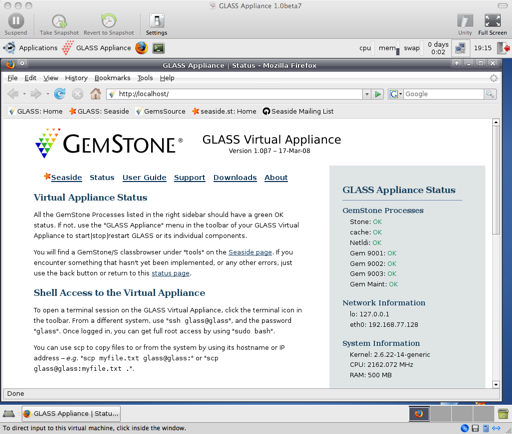
\includegraphics[width=0.6\textwidth]{f9/gk0p8cwy7j2qiy4nw7paibnjwkimhs/gemstone-status-page.png}
		\caption{GLASS Virtual Appliance status page.\label{book:gettingstarted:gemstone:usingglassva:statuspage}}
	\end{center}
\end{figure}


We recommend when you are ready to stop work, you suspend the appliance rather than shut it down. This will make the next startup much faster. You'll be able to start up just where you left off.

The status of your GemStone$/$S system is refreshed every 10 seconds. All the GemStone processes listed in the right sidebar should have a green OK status as shown in \autoref{book:gettingstarted:gemstone:usingglassva:statuspanel}. If not, use the ``GLASS Appliance'' menu shown in \autoref{book:gettingstarted:gemstone:usingglassva:glassmenu} to start, stop, or restart GLASS or its individual components. 

\begin{figure}[h!tbp]
	\begin{center}
		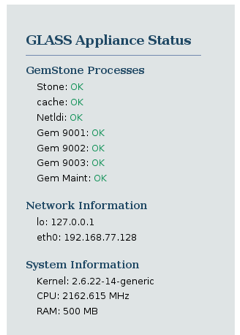
\includegraphics[width=0.3\textwidth]{6a/py5wibhf1almb9kvtc9pf3vi6h6mx1/gemstone-status-panel.png}
		\caption{GLASS Virtual Appliance status.\label{book:gettingstarted:gemstone:usingglassva:statuspanel}}
	\end{center}
\end{figure}


You should now be able to explore the Seaside components installed in the GLASS Virtual appliance by clicking on the \symbol{34}GLASS:  Seaside\symbol{34} bookmark you can see in \autoref{book:gettingstarted:gemstone:usingglassva:seasidedispatcher}. You can also view that web page from another computer on your network by using the \symbol{34}eth0:\symbol{34} IP address listed under \symbol{34}Network Information\symbol{34}.

\begin{figure}[h!tbp]
	\begin{center}
		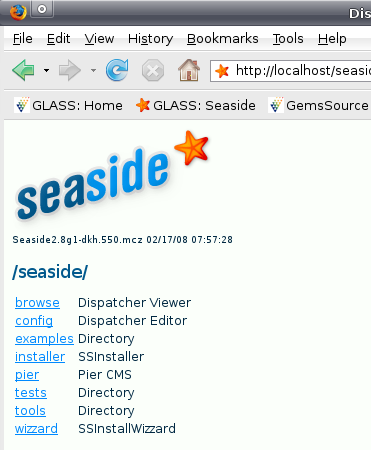
\includegraphics[width=0.3\textwidth]{48/jevfunzfm0ft9tldrauxb9alwg470w/gemstone-seaside-dispatcher.png}
		\caption{GLASS Virtual Appliance Seaside page.\label{book:gettingstarted:gemstone:usingglassva:seasidedispatcher}}
	\end{center}
\end{figure}


Should you need to edit a file or perform other command line operations on the appliance, you can open a terminal session by clicking on the terminal icon in the toolbar. If you prefer, you can \ct{ssh} to the appliance by using the IP address mentioned above and the username$/$password glass$/$glass. To copy files to$/$from the appliance use the \ct{scp} command. Here's an example of using \ct{scp} to copy a seaside log file from the appliance to your current directory.

\Needspace{1\baselineskip}
\begin{lstlisting}
scp glass@192.168.77.128:/opt/gemstone/log/seaside.log .
\end{lstlisting}

\begin{figure}[h!tbp]
	\begin{center}
		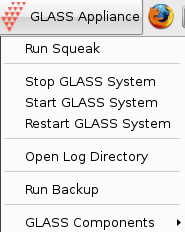
\includegraphics[width=0.2\textwidth]{75/ks5pyqw10qn5bksi9kcqze4314wezf/gemstone-glass-menu.png}
		\caption{GLASS Virtual Appliance menu.\label{book:gettingstarted:gemstone:usingglassva:glassmenu}}
	\end{center}
\end{figure}


% /book/getting-started/gemstone/developing-component
\section{A First Seaside Component}
\label{book:gettingstarted:gemstone:developingcomponent}

Let's build the counter application in GemStone$/$S. We'll be using a Squeak GUI as a development environment for GemStone$/$S. While this is quite similar to developing in Squeak, you will notice a few differences. 

The most important difference developers need to be aware of is is due to GemStone$/$S being a multi-user object database with \href{http://en.wikipedia.org/wiki/ACID}{ACID transaction properties}. Each GemStone$/$S VM sees a consistent state of the database in isolation from intermediate changes underway in any other VM. Those changes cannot be seen until they are committed to the database. This is handled automatically in your Seaside application since the GemStone$/$S Seaside framework immediately commits any data sent from a web client to the GemStone$/$S application server. However, \textit{when writing code, you must manually commit before that code can be used or or even seen by other VM's}. Conversely, if you decide you've made a mistake, you can abort and your code changes will be erased. 

Start by selecting \symbol{34}Run Squeak\symbol{34} in the \symbol{34}GLASS Appliance\symbol{34} menu in the toolbar. This will open a Squeak image containing a GemStone$/$S Login window (\autoref{book:gettingstarted:gemstone:developingcomponent:loginwindow}). Click on the \symbol{34}Login\symbol{34} button, type your initials into the box that pops up, than click \symbol{34}accept\symbol{34}. This will open a GemStone$/$S Transcript window (\autoref{book:gettingstarted:gemstone:developingcomponent:transcriptwindow}). The text pane in the GemStone$/$S Transcript window is actually a workspace and not a transcript. This will be changed in the next release when this window is reimplemented in OmniBrowser.

\begin{figure}[h!tbp]
	\begin{center}
		\includegraphics[width=0.4\textwidth]{16/shaurt3iaizv5bf490iehaiyeo31ku/gemstone-login-window.png}
		\caption{GemStone$/$S Login window.\label{book:gettingstarted:gemstone:developingcomponent:loginwindow}}
	\end{center}
\end{figure}


\begin{figure}[h!tbp]
	\begin{center}
		\includegraphics[width=0.6\textwidth]{04/8h6b7qvu3aw7u0z9tdbqdrqn2qoqqj/gemstone-transcript-window.png}
		\caption{GemStone$/$S Transcript window.\label{book:gettingstarted:gemstone:developingcomponent:transcriptwindow}}
	\end{center}
\end{figure}


% /book/getting-started/gemstone/developing-component/defining-component
\subsection{Defining a Component}
\label{book:gettingstarted:gemstone:developingcomponent:definingcomponent}

There are two ways to define the new \ct{WebCounter} subclass of \ct{WAComponent}.

Type the following class definition into the GemStone$/$S Transcript window or a GemStone workspace, then type CTL-d or use the \symbol{34}doit\symbol{34} menu item. Note that this GemStone$/$S class definition is slightly different than it would be in Squeak. The Squeak form works equally well, however you'll always see class definitions in the GemStone$/$S form when you browse the class.

\Needspace{3\baselineskip}
\begin{lstlisting}
WAComponent subclass: 'WebCounter'
    instVarNames: #(count)
    classVars: #()
    classInstVars: #()
    poolDictionaries: #[]
    category: 'GettingStarted'
\end{lstlisting}

\begin{figure}[h!tbp]
	\begin{center}
		\includegraphics[width=0.6\textwidth]{38/a120qck273cibwfnb77c29sgakd8ny/gemstone-wacomponent-subclass.png}
		\caption{WAcomponent subclass template.\label{book:gettingstarted:gemstone:developingcomponent:definingcomponent:wacomponentsubclass}}
	\end{center}
\end{figure}


Alternatively, open a GemStone$/$S System Browser on the class \ct{WAComponent} and fill in a \symbol{34}subclass template\symbol{34} as shown in \autoref{book:gettingstarted:gemstone:developingcomponent:definingcomponent:wacomponentsubclass}. To do this, click the green \symbol{34}Browse\symbol{34} button in the GemStone$/$S Transcript window, and type WAComponent into the popup. Left click WAComponent and then select the \symbol{34}subclass template\symbol{34} menu item. After filling in the template with the class definition above, type CTL-s or select the \symbol{34}accept\symbol{34} menu item.

% /book/getting-started/gemstone/developing-component/defining-methods
\subsection{Defining Some Methods}
\label{book:gettingstarted:gemstone:developingcomponent:definingmethods}

Now we define some instance methods to initialize the value of the counter to zero , and to increment or decrement  the value of the counter.

While it is not strictly necessary, it can be useful to define categories for methods you add. Middle button click on the all as shown in \autoref{book:gettingstarted:gemstone:developingcomponent:definingmethods:createcategory}, select \symbol{34}create category\symbol{34} and type in a category name. If you select a method category, new methods will appear in that category.

\begin{figure}[h!tbp]
	\begin{center}
		\includegraphics[width=0.6\textwidth]{bd/8z9n19i0s68bm89qurca9tx9vnp6e9/gemstone-create-category.png}
		\caption{Create a category.\label{book:gettingstarted:gemstone:developingcomponent:definingmethods:createcategory}}
	\end{center}
\end{figure}


\Needspace{3\baselineskip}
\begin{lstlisting}
WebCounter>>initialize
    super initialize.
    count := 0
\end{lstlisting}

\Needspace{2\baselineskip}
\begin{lstlisting}
WebCounter>>increase
    count := count + 1
\end{lstlisting}

\Needspace{2\baselineskip}
\begin{lstlisting}
WebCounter>>decrease
    count := count - 1
\end{lstlisting}

At this point it would be a good idea to commit your changes to the database. Click the commit button in the transcript window. You should always commit any changes to your code before logging out of GemStone, just as you would save a text document in an editor before logging off of your computer. If you want to throw away any code created or modified since your last commit, click the abort button instead.

% /book/getting-started/gemstone/developing-component/rendering-counter
\subsection{Rendering a counter}
\label{book:gettingstarted:gemstone:developingcomponent:renderingcounter}

In order to render the counter in a web browser, we must create a  \ct{WAComponent$>$$>$renderContentOn:}  method. The following method will display the value of the variable \ct{count} as an HTML heading.

\Needspace{2\baselineskip}
\begin{lstlisting}
WebCounter>>renderContentOn: html
    html heading: count.
\end{lstlisting}

% /book/getting-started/gemstone/developing-component/register-application
\subsection{Registering the Application}
\label{book:gettingstarted:gemstone:developingcomponent:registerapplication}

Before you can access the counter application from your web browser, you must register it with Seaside. Type the following code into a Transcript or Workspace and then type CTRL-d or use the \symbol{34}doit\symbol{34} menu item. Afterwards, make sure to commit your code.

\Needspace{1\baselineskip}
\begin{lstlisting}
WebCounter registerAsApplication: 'WebCounter'.
\end{lstlisting}

Note that this expression can also be added in the class \ct{initialize} method which is invoked at the time the class is loaded in memory as shown below.

\Needspace{2\baselineskip}
\begin{lstlisting}
WebCounter class>>initialize
    self registerAsApplication: 'WebCounter'
\end{lstlisting}

Now you can launch the application in your web browser by visiting 
\href{http://localhost/seaside/WebCounter}{http:$/$$/$localhost$/$seaside$/$WebCounter}, see \autoref{book:gettingstarted:gemstone:developingcomponent:registerapplication:countersimple}.

\begin{figure}[h!tbp]
	\begin{center}
		\includegraphics[width=0.6\textwidth]{dd/z6ip03isny7nivetdvac2x0fbffnq6/gemstone-counter-simple.png}
		\caption{A simple counter.\label{book:gettingstarted:gemstone:developingcomponent:registerapplication:countersimple}}
	\end{center}
\end{figure}


% /book/getting-started/gemstone/developing-component/adding-behavior
\subsection{Adding Behavior}
\label{book:gettingstarted:gemstone:developingcomponent:addingbehavior}

Now we can add some actions by defining callbacks attached to anchors, see \autoref{book:gettingstarted:gemstone:developingcomponent:addingbehavior:counterwithactions}. A callback is a piece of code that will be executed when a link is clicked. We will explain this in detail later in the book. 
Modify the method \ct{WAComponent$>$$>$renderContentOn:} as follows and commit your changes. 

\Needspace{3\baselineskip}
\begin{lstlisting}
WebCounter>>renderContentOn: html
    html heading: count.
    html anchor 
        callback: [ self increase ];
        with: '++'.
    html space.
    html anchor
        callback: [ self decrease ];
        with: '--'
\end{lstlisting}

Now when you click on the links you will see the counter increment or decrement.

\begin{figure}[h!tbp]
	\begin{center}
		\includegraphics[width=0.6\textwidth]{3c/8ih6bx7tz6lius6vvagr9edbmn3h09/gemstone-counter-with-actions.png}
		\caption{A simple counter with increment and decrement actions.\label{book:gettingstarted:gemstone:developingcomponent:addingbehavior:counterwithactions}}
	\end{center}
\end{figure}


% /book/getting-started/gemstone/updating
\section{Keeping Up With the Latest Features}
\label{book:gettingstarted:gemstone:updating}

We regularly update the Seaside features of GemStone$/$S between major product releases. These are usually announced in Dale's blog at \href{http://gemstonesoup.wordpress.com/}{http:$/$$/$gemstonesoup.wordpress.com$/$}. It's important to load Monticello packages in the sequence below to ensure the GLASS package in GemStone$/$S and the GemStone package in Squeak are in sync.

\textbf{Step 1.} Load the latest GLASS-dkh into GemStone from \href{http://seaside.gemstone.com/ss/GLASS}{http:$/$$/$seaside.gemstone.com$/$ss$/$GLASS}. This loads a large number of packages so it takes minutes to complete even on a fast connection. Be patient.

To load a Monticello package into GemStone$/$S, click the green \symbol{34}Monticello\symbol{34} button in the Transcript or Workspace window. Highlight the package name in the left pane (\autoref{book:gettingstarted:gemstone:updating:monticellobrowser}), the URL starting with \href{http://seaside.gemstone.com/ss/}{http:$/$$/$seaside.gemstone.com$/$ss$/$} in the right pane, and then click the \symbol{34}open\symbol{34} button. This will open a Monticello repository browser. Highlight the package name in the left pane (\autoref{book:gettingstarted:gemstone:updating:monticellorepository}) and the package version in the right pane. Check the comments on the package for any precautions on compatibility before loading -- you could need to use an earlier package.

\begin{figure}[h!tbp]
	\begin{center}
		\includegraphics[width=0.6\textwidth]{56/r9vc03upbsceikb7nfknqnipku59uq/gemstone-monticello-browser.png}
		\caption{GemStone Monticello browser.\label{book:gettingstarted:gemstone:updating:monticellobrowser}}
	\end{center}
\end{figure}


\begin{figure}[h!tbp]
	\begin{center}
		\includegraphics[width=0.6\textwidth]{24/0nfka161ri9khys8u23kdvqpeg856j/gemstone-monticello-repository.png}
		\caption{GemStone Monticello repository.\label{book:gettingstarted:gemstone:updating:monticellorepository}}
	\end{center}
\end{figure}


After updating, it's a good idea to click the green \symbol{34}Test Runner\symbol{34} button in the Transcript window, and then click \symbol{34}Run Selected\symbol{34}. If all the tests pass (\autoref{book:gettingstarted:gemstone:updating:testrunner}), commit your transaction. If some fail, it's probably simpler to abort rather than debug the problem. 

Then log completely out of GemStone, or the next step will not succeed.

\textbf{Step 2.} Load the latest GemStone-dkh into Squeak from
\href{http://seaside.gemstone.com/ss/GemStone}{http:$/$$/$seaside.gemstone.com$/$ss$/$GemStone}. 

Then you can log back in to GemStone. 

Loading a Monticello package into Squeak is similar (\autoref{book:gettingstarted:gemstone:updating:squeakmonticello}), but you start by opening a Squeak Monticello browser rather than a GemStone$/$S one. It's important to remember Squeak and GemStone$/$S are two different systems. Even though they can run much of the same Smalltalk code, it's important to load your code into the one you intended.

\begin{figure}[h!tbp]
	\begin{center}
		\includegraphics[width=0.6\textwidth]{75/l5ftlafztvnztkboibn4uhpgyup530/gemstone-squeak-monticello.png}
		\caption{Squeak Monticello repository.\label{book:gettingstarted:gemstone:updating:squeakmonticello}}
	\end{center}
\end{figure}


\begin{figure}[h!tbp]
	\begin{center}
		\includegraphics[width=0.6\textwidth]{7e/pjg26wq3q728a0aayqu7baghubyi6a/gemstone-test-runner.png}
		\caption{Making sure tests pass.\label{book:gettingstarted:gemstone:updating:testrunner}}
	\end{center}
\end{figure}


% /book/getting-started/gst
\chapter{GNU Smalltalk}
\label{book:gettingstarted:gst}

\begin{blockquote}
\textit{by Paolo Bonzini, developer of GNU Smalltalk}

\end{blockquote}

In this section we describe how to get started developing a Seaside application in GNU Smalltalk. We assume that you already have the 3.0a version (or a later one) of GNU Smalltalk installed. This is the latest release at the time of this writing, and the first to include support for Seaside. 

To download it, follow instructions at \href{http://smalltalk.gnu.org/download}{http:$/$$/$smalltalk.gnu.org$/$download}.

% /book/getting-started/gst/load-seaside
\section{Creating a GNU Smalltalk image with Seaside loaded}
\label{book:gettingstarted:gst:loadseaside}

Seaside support is split into a number of separately loadable packages. Here are the ones that are available in GNU Smalltalk 3.0a:

\begin{itemize}
\item  Seaside-Core
\item  Seaside-Adapters-Swazoo
\item  Seaside-Development
\item  Seaside-Examples
\end{itemize}

The Seaside package is a collective package that loads the first two.

First of all, you should create a new image with the package loaded. In GNU Smalltalk, the image acts as a kind of cache and preloading the package will speed up further operation. 

In the remainder of this section, \ct{\$} is used as the prompt for things you type at the shell, and \ct{st$>$} is used as the prompt for things you type for GNU Smalltalk.

\Needspace{3\baselineskip}
\begin{lstlisting}
$ gst
st> PackageLoader fileInPackage: 'Seaside'
st> PackageLoader fileInPackage: 'Seaside-Development'
st> PackageLoader fileInPackage: 'Seaside-Examples'
st> ObjectMemory snapshot: 'seaside.im'
\end{lstlisting}

% /book/getting-started/gst/remote-vm
\section{Operating the GNU Smalltalk virtual machine remotely}
\label{book:gettingstarted:gst:remotevm}

At the end of the previous section you created a new image from the GNU Smalltalk read-eval-print loop. If you're familiar with other Smalltalk, it is a sort of console-based Transcript; if you're familiar with other scripting languages you will have already recognized it.

From now on, however, you will run Seaside applications within a remote-controlled instance of GNU Smalltalk, running in background as a daemon. The following three commands start the daemon, print the daemon's process id, and finally stop the daemon.

\Needspace{3\baselineskip}
\begin{lstlisting}
$ gst-remote -I seaside.im --daemon
$ gst-remote --pid
$ gst-remote --kill
\end{lstlisting}

The first command has the \ct{--daemon} command-line option, and hence starts an instance of GNU Smalltalk that will run in the background and will be used to serve web pages. The other two don't have the command-line option, and all they do is interacting with the background instance of GNU Smalltalk. Note that you don't need to specify the image unless you are starting the background instance of GNU Smalltalk, because only the background virtual machine needs to have the Seaside packages loaded.

Now, let's start the daemon again and also start the web server:

\Needspace{2\baselineskip}
\begin{lstlisting}
$ gst-remote -I seaside.im --daemon
$ gst-remote --start=Seaside
\end{lstlisting}

Seaside is now serving on \href{http://localhost:8080/}{http:$/$$/$localhost:8080$/$}; the entry address is by default \href{http://localhost:8080/seaside}{http:$/$$/$localhost:8080$/$seaside}. Try visiting the \href{http://localhost:8080/seaside/examples/counter}{http:$/$$/$localhost:8080$/$seaside$/$examples$/$counter} URL to make sure that the system works.

You can stop and restart the server without killing the daemon by running:

\Needspace{1\baselineskip}
\begin{lstlisting}
$ gst-remote --stop=Seaside
\end{lstlisting}

Be sure to restart serving web pages after running this command.

Another common operation is loading a file into the remote GNU Smalltalk instance. You do this using the following expression.

\Needspace{1\baselineskip}
\begin{lstlisting}
$ gst-remote --file FILENAME.st
\end{lstlisting}

You can also control an instance of GNU Smalltalk that's running in background using \ct{gst-remote --eval}. After \ct{--eval} you put a Smalltalk command that is executed within the server, for example:

\Needspace{1\baselineskip}
\begin{lstlisting}
$ gst-remote --eval '100 factorial printNl'
\end{lstlisting}

will compute \textit{100!} in the background image and print the result.

 \ct{gst-remote} supports running commands on a virtual machine running on a different machines, by specifying a hostname right after the command name itself. Note that, in this case, arguments to \ct{--file} still refer to paths on the \textit{local} machine.

% /book/getting-started/gst/developing
\section{Developing in GNU Smalltalk}
\label{book:gettingstarted:gst:developing}

Developers who are already familiar with other scripting languages, for example Ruby, will have few problems adapting to GNU Smalltalk.

A relatively important difference from other Smalltalk dialects is the availability of namespaces, a mechanism for restricting the referential scope of such names. While advanced usage of name spaces can be quite involved, in practice it is relatively simple and based on a few essential points.

\begin{itemize}
\item  The top-level name space is named Smalltalk. 
\item  All classes and add-ons are defined in sub-namespaces of Smalltalk.
\item  Most Seaside classes are in the namespace named Seaside. 
\end{itemize}

Your application should, in general, be in a namespace that you create for your own usage. If you use the package system of GNU Smalltalk, switching to a separate namespace is actually done automatically while loading the package.

However, for simplicity especially during early development, you can define your classes directly in the Smalltalk name space.

% /book/getting-started/gst/first-component
\section{Developing your first component}
\label{book:gettingstarted:gst:firstcomponent}

To illustrate the above points, we will go through the initial steps of developing the Counter example in GNU Smalltalk. We'll use a slightly different name so we won't conflict with the example already loaded with Seaside.

Place the following code in a file:

\Needspace{3\baselineskip}
\begin{lstlisting}
Seaside.WAComponent subclass: WebCounter [
    | count |
    WebCounter class >> canBeRoot [ ^true ]

    initialize [
        super initialize.
        count := 0.
    ]
    states [ ^{ self } ]
    renderContentOn: html [ html heading: count ]
]
\end{lstlisting}

\Needspace{1\baselineskip}
\begin{lstlisting}
WebCounter registerAsApplication: 'webcounter'
\end{lstlisting}

You can see that, apart from some syntactic sugar, the above is just Smalltalk as in any other dialect, except that method bodies are surrounded by square brackets. \ct{count} declares an instance variable.

Here are the few concepts that the above basic component highlights:

\begin{itemize}
\item  A Seaside component, is defined by a subclass of \ct{WAComponent} class. Accordingly, to create a component, the above file creates the corresponding class.
\item  Each component is responsible for rendering itself in the web browser. This is done in Seaside by implementing a \ct{renderContentOn:} method. In this simple case, that means displaying the counter value.
\item  Registering the application with Seaside makes its entry point is accessible at a URL path.
\end{itemize}

Registering an application is done in two steps. First, we must declare that our application component can be a root component, by defining a \ct{WAComponent class$>$$>$canBeRoot} class method. Second, we must register the component as an application, which is done by the final line of the file. Code that is outside a class declaration corresponds to a \textit{doit} (or, if you are not coming from Smalltalk, is just evaluated as the file is parsed).

After loading the code in a running server:

\Needspace{1\baselineskip}
\begin{lstlisting}
$ gst-remote --file Counter.st
\end{lstlisting}

the application will be visible at \href{http://localhost:8080/seaside/webcounter}{http:$/$$/$localhost:8080$/$seaside$/$webcounter}. At the moment however it is pretty boring, so we improve the \ct{WAComponent$>$$>$renderContentOn:} method like this:

\Needspace{3\baselineskip}
\begin{lstlisting}
    renderContentOn: html [
        html heading: count.
        html anchor callback: [ count := count + 1 ]; with: '++'.
        html space.
        html anchor callback: [ count := count - 1 ]; with: '--'.
    ]
\end{lstlisting}

Reload the code in the server using the same \ct{gst-remote} invocation as above. Go back to the web browser and refresh the page: there are now two anchors with increment (++) and decrement (--) links that call back to the actions.

Click the new links a few time to verify that it works. That's it. You developed your first Seaside component.

% /book/getting-started/va-smalltalk
\chapter{VA Smalltalk}
\label{book:gettingstarted:vasmalltalk}

\begin{blockquote}
\textit{by John O'Keefe, Principal Software Architect, Instantiations Inc.}

\end{blockquote}

In this section we will show you how to get started developing Seaside applications with VA Smalltalk. First we will discuss how to obtain and install Seaside. Then we will show you how to develop your first application: a simple counter.

% /book/getting-started/va-smalltalk/installation
\section{Loading Seaside into VA Smalltalk}
\label{book:gettingstarted:vasmalltalk:installation}

Seaside was first delivered as part of the VA Smalltalk V8.0 release.  You can download the latest VA Smalltalk release from the Instantiations download site at \href{http://www.instantiations.com/VAST/download/}{http:$/$$/$www.instantiations.com$/$VAST$/$download$/$}. After installing VA Smalltalk, start the development image.

Seaside support is provided as a loadable feature in VA Smalltalk.  From the Transcript, select \textit{Tools $|$ Load$/$Unload Features...} to open the Feature Loader, see \autoref{book:gettingstarted:vasmalltalk:installation:featureloader}.

\begin{figure}[h!tbp]
	\begin{center}
		\includegraphics[width=0.6\textwidth]{74/liio52aj33lf874yp75ymlburcqsh0/FeatureLoader.png}
		\caption{VA Smalltalk Feature Loader.\label{book:gettingstarted:vasmalltalk:installation:featureloader}}
	\end{center}
\end{figure}


Scroll down to the \textit{ST: Seaside Core} feature, select it, and use the \textit{$>$$>$} button to mark it for loading. You can see other Seaside features in the list that you may also want to load.  When you have selected all the features you want to load, and have moved them to the Loaded features list, select the \textit{OK} button to load the features into your image.

% /book/getting-started/va-smalltalk/using
\section{Starting VA Smalltalk Seaside}
\label{book:gettingstarted:vasmalltalk:using}

Once you have the VA Smalltalk image running and Seaside loaded, you can start a Seaside Server.  From the Transcript, select \textit{Tools $|$ Open Seaside Control Panel} to open the Seaside Control Pane, see \autoref{book:gettingstarted:vasmalltalk:using:initialcontrolpanel}.

\begin{figure}[h!tbp]
	\begin{center}
		\includegraphics[width=0.6\textwidth]{29/lt6iy338un8wuvdehyr619lvqk8jgd/OpenSeasideControlPanel.png}
		\caption{Open Seaside Control Panel.\label{book:gettingstarted:vasmalltalk:using:initialcontrolpanel}}
	\end{center}
\end{figure}


% /book/getting-started/va-smalltalk/using/control-panel
\subsection{Seaside Server Control Panel Menu Options}
\label{book:gettingstarted:vasmalltalk:using:controlpanel}

The Seaside Server Control Panel is the central control point for Seaside Servers.  When the Seaside Server Control Panel is first opened it is empty, see \autoref{book:gettingstarted:vasmalltalk:using:controlpanel:controlpanel}.

\begin{figure}[h!tbp]
	\begin{center}
		\includegraphics[width=0.6\textwidth]{f5/zfs2fzvj71bvs1drsfadp8r968kn0j/control-panel.png}
		\caption{Initial Seaside Server Control Panel.\label{book:gettingstarted:vasmalltalk:using:controlpanel:controlpanel}}
	\end{center}
\end{figure}


The menu on the control panel provides options to manage server adaptors and to configure the control panel.  The options are:

\textbf{Manage}

\begin{tabularx}{\textwidth}{lX}
 \textit{Add adaptor...} &  Create a new server\\
 \textit{Start All} & Start all the servers that are not currently running\\
 \textit{Stop All} & Stop all the servers that are currently running\\
 \textit{Start} & Start the selected server(s)\\
 \textit{Stop} & Stop the selected server(s)\\
 \textit{Remove} & Remove the selected server(s) -- they must be in the stopped state\\
 \textit{Inspect} & Open a VA Smalltalk inspector on the selected server\\
 \textit{Use new dispatcher} &\\
 \textit{Clear configuration caches} &\\
 \textit{Clear sessions} &\\
\end{tabularx}
\textbf{Configure}

\begin{tabularx}{\textwidth}{lX}
 \textit{Default port ...} & The default port used when adding a server adaptor\\
 \textit{Control Panel refresh interval ...} & The frequency of refreshing the control panel information.  It is specified in seconds; a value of 0 turns off refresh.\\
 \textit{Reset to defaults} & Reset the default port to 8080 and the refresh interval to 5 seconds\\
\end{tabularx}

% /book/getting-started/va-smalltalk/using/add-server
\subsection{Adding a Server Adaptor}
\label{book:gettingstarted:vasmalltalk:using:addserver}

Select \textit{Manage $|$ Add adaptor ...} to add an adaptor that will serve Seaside pages, see \autoref{book:gettingstarted:vasmalltalk:using:addserver:addadaptor}. The added Server Adaptor will be in the stopped state.
  
\begin{figure}[h!tbp]
	\begin{center}
		\includegraphics[width=0.6\textwidth]{33/zmjzbm36q80d7flhswdtrq8gueqoci/addadaptor.png}
		\caption{Seaside Server Control Panel Add Adaptor.\label{book:gettingstarted:vasmalltalk:using:addserver:addadaptor}}
	\end{center}
\end{figure}


In the Add Server Adaptor dialog you can select the Server Adaptor class (currently only one class is available) and the port used to connect to the server, see \autoref{book:gettingstarted:vasmalltalk:using:addserver:addadaptordialog}.

\begin{figure}[h!tbp]
	\begin{center}
		\includegraphics[width=0.6\textwidth]{d2/9dijcjoofmbjzvkgzyxhsxk61ioz1e/add-adaptor-dialog.png}
		\caption{Add Seaside Server Adaptor Dialog.\label{book:gettingstarted:vasmalltalk:using:addserver:addadaptordialog}}
	\end{center}
\end{figure}


You can add multiple server adaptors which can listen on different ports.

% /book/getting-started/va-smalltalk/using/start-server
\subsection{Starting a Server Adaptor}
\label{book:gettingstarted:vasmalltalk:using:startserver}

Once you have added a server adaptor to the Seaside Server Control Panel, you can start that server adaptor.  Select the server you want to start; then select \textit{Manage $|$ Start} from the menu bar, see \autoref{book:gettingstarted:vasmalltalk:using:startserver:startserveradaptor}. Alternatively you might want to use \textit{Manage $|$ Start All} to start all the server adaptors.

\begin{figure}[h!tbp]
	\begin{center}
		\includegraphics[width=0.6\textwidth]{b5/rr3mjy5oa5qmjnk0aujghqp4qccgty/start.png}
		\caption{Start Server Adaptor.\label{book:gettingstarted:vasmalltalk:using:startserver:startserveradaptor}}
	\end{center}
\end{figure}


At this point Seaside is running and ready to serve web pages, see \autoref{book:gettingstarted:vasmalltalk:using:startserver:startedserveradaptor}.

\begin{figure}[h!tbp]
	\begin{center}
		\includegraphics[width=0.6\textwidth]{3e/5vkabgq8lnk4v2ug3b8smp9blwdiz9/started.png}
		\caption{Started Server Adaptor.\label{book:gettingstarted:vasmalltalk:using:startserver:startedserveradaptor}}
	\end{center}
\end{figure}


% /book/getting-started/va-smalltalk/using/simple-example
\subsection{A Simple Seaside Example}
\label{book:gettingstarted:vasmalltalk:using:simpleexample}

At this point you have a running Seaside Server.  Now you can try a simple example shipped with Seaside.  In a browser, enter the following URL: 
 \href{http://localhost:8080/examples/counter}{http:$/$$/$localhost:8080$/$examples$/$counter} to see the pre-built counter application. You should see something like the page presented in \autoref{book:gettingstarted:vasmalltalk:using:simpleexample:counter}.

\begin{figure}[h!tbp]
	\begin{center}
		\includegraphics[width=0.6\textwidth]{9f/btjhw3ffugwcjj3lquhdchqih48ayg/counter.png}
		\caption{Sample Counter.\label{book:gettingstarted:vasmalltalk:using:simpleexample:counter}}
	\end{center}
\end{figure}


Selecting the \textit{++} or \textit{--} links will increment or decrement the counter.  Later in this section you will build a Seaside application similar to this example.

% /book/getting-started/va-smalltalk/first-component
\section{Developing Your First Seaside Component}
\label{book:gettingstarted:vasmalltalk:firstcomponent}

Now you are ready to write your first Seaside component. You will code a simple counter in several steps: define an application and a class, define state, and define how the component is rendered. Finally you will declare it as a Seaside application.

% /book/getting-started/va-smalltalk/first-component/define-component
\subsection{Defining a Component}
\label{book:gettingstarted:vasmalltalk:firstcomponent:definecomponent}

First we will define a new VA Smalltalk application to hold our simple counter. We create the SampleSeasideApp application using VA Smalltalk's Applications Manager.  Select \textit{Applications $|$ Create $|$ Application...} to specify the name of the new application, see \autoref{book:gettingstarted:vasmalltalk:firstcomponent:definecomponent:VASmalltalkApplicationManager}.

\begin{figure}[h!tbp]
	\begin{center}
		\includegraphics[width=0.6\textwidth]{31/jydnmrpoip3qrxmupcw5hxt4qbmkwl/VASTAppMgr.png}
		\caption{VASmalltalkApplicationManager.\label{book:gettingstarted:vasmalltalk:firstcomponent:definecomponent:VASmalltalkApplicationManager}}
	\end{center}
\end{figure}


You will also need to specify the prerequisite applications for your new application.  We are going to use the \ct{WAAdmin}' tool to manage the application, so you should specify its application (\ct{SeasideToolsCoreApp}) as the only direct prerequisite of your new application.

Now we define a new Seaside component named \ct{WebCounter} by defining a subclass of \ct{WAComponent}. You can do this by selecting \textit{Classes $|$ Add $|$ New Class...}.  Select \ct{WAComponent} as the superclass of your new class and select \textit{OK}; enter the name of your new class (\ct{WebCounter}) and select \textit{OK}; finally, select \textit{subclass} as the type of subclass you are creating and select \textit{OK}.  At this point you have created an application with 2 classes in it, \ct{SampleWebApp} and \ct{WebCounter}.

Now open a browser on the \ct{WebCounter} class and add an instance variable that will contain the state of the counter.  The class definition should look like this:

\Needspace{3\baselineskip}
\begin{lstlisting}
WAComponent subclass: #WebCounter
    instanceVariableNames: 'count'
    classVariableNames: ''
    poolDictionaries: ''
\end{lstlisting}

% /book/getting-started/va-smalltalk/first-component/adding-methods
\subsection{Adding Some Methods}
\label{book:gettingstarted:vasmalltalk:firstcomponent:addingmethods}

Now we define some instance methods to initialize and change the value of the counter.

\Needspace{3\baselineskip}
\begin{lstlisting}
WebCounter>>initialize
   super initialize.
   count := 0
\end{lstlisting}

\Needspace{2\baselineskip}
\begin{lstlisting}
WebCounter>>increase
    count := count + 1
\end{lstlisting}

\Needspace{2\baselineskip}
\begin{lstlisting}
WebCounter>>decrease
    count := count - 1
\end{lstlisting}

% /book/getting-started/va-smalltalk/first-component/rendering-counter
\subsection{Rendering a Counter}
\label{book:gettingstarted:vasmalltalk:firstcomponent:renderingcounter}

Now we define the instance method \ct{renderContentOn:} to display the counter as a heading. Seaside will call such a method when it needs to display a component in the web browser. In the following method we just say that we want to display the value of the variable \ct{count} using a heading HTML tag.

\Needspace{2\baselineskip}
\begin{lstlisting}
WebCounter>>renderContentOn: html
    html heading: count
\end{lstlisting}

As you see, in Seaside you do not directly write HTML but rather you use a higher-level interface that models HTML.  This helps you avoid making HTML mistakes.  We will go into much more detail on this subject later in the book.

% /book/getting-started/va-smalltalk/first-component/registering
\subsection{Registering the Counter Component}
\label{book:gettingstarted:vasmalltalk:firstcomponent:registering}

Now we should register the component as an application so that we can access it directly from the url path that will be associated with it. To register a component as an application, we ask the administration interface class \ct{WAAdmin} to do the work for us:

\Needspace{1\baselineskip}
\begin{lstlisting}
WAAdmin register: WebCounter asApplicationAt: 'webcounter'
\end{lstlisting}

will register the component \ct{WebCounter} as the application named \ct{webcounter}.

Note that this expression can also be added in the \ct{WebCounter} \textit{class} method \ct{initialize} which is invoked when the class is loaded into memory:

\Needspace{2\baselineskip}
\begin{lstlisting}
WebCounter class>>initialize
    WAAdmin register: self asApplicationAt: 'webcounter'
\end{lstlisting}

Now you can launch the application in your web browser by going to \href{http://localhost:8080/webcounter}{http:$/$$/$localhost:8080$/$webcounter}, see \autoref{book:gettingstarted:vasmalltalk:firstcomponent:registering:simplecounter}.

\begin{figure}[h!tbp]
	\begin{center}
		\includegraphics[width=0.6\textwidth]{e2/d0fh33ib9jbum5nlyrmp77q9p45ch7/va-simple-counter.png}
		\caption{Simple-counter.\label{book:gettingstarted:vasmalltalk:firstcomponent:registering:simplecounter}}
	\end{center}
\end{figure}


% /book/getting-started/va-smalltalk/first-component/adding-behavior
\subsection{Adding Behavior to the Counter}
\label{book:gettingstarted:vasmalltalk:firstcomponent:addingbehavior}

Now we can add some actions by defining callbacks attached to anchors. We will explain actions in detail later in this book. A callback is a piece of code that will be executed when a link is clicked. For now this is just to give you a feel of Seaside programming. We update the \ct{WebCounter$>$$>$renderContentOn:} method as follows.

\Needspace{3\baselineskip}
\begin{lstlisting}
WebCounter>>renderContentOn: html
    html heading: count.
    html anchor 
        callback: [ self increase ];
        with: '++'.
    html space.
    html anchor
        callback: [ self decrease ];
        with: '--'
\end{lstlisting}

After saving your changes, refresh the browser page and you will now see the increment and decrement links.  Click on the links so see that the counter get incremented or decremented, see \autoref{book:gettingstarted:vasmalltalk:firstcomponent:addingbehavior:VASTsamplecounterwithactions}.

\begin{figure}[h!tbp]
	\begin{center}
		\includegraphics[width=0.6\textwidth]{34/s2qncrc6bu4vj3c2r6sxaewk5jzxnr/VASTwebcounter.png}
		\caption{VAST sample counter with actions.\label{book:gettingstarted:vasmalltalk:firstcomponent:addingbehavior:VASTsamplecounterwithactions}}
	\end{center}
\end{figure}


% /book/fundamentals
\part{Fundamentals}
\label{book:fundamentals}

In this part we will introduce you to the manipulation of basic elements such as texts, anchors and callbacks as well as forms. It presents the notion of \textit{brushes} that is central to the Seaside API. Understanding these concepts will be fundamental to your use of Seaside.

% /book/fundamentals/rendering-components
\chapter{Rendering Components}
\label{book:fundamentals:renderingcomponents}

In this chapter you will learn the basics of displaying text and other information such as tables and lists with Seaside and its powerful XHTML manipulation interface. You will learn how to create a \textit{component} which could include text, a form, a picture, or anything else that you would like to display in a web browser. Seaside's component framework is one of its most powerful features and writing an application in Seaside amounts to creating and manipulating components. You will learn how to use Seaside's API, which is based on the concept of ``brushes'', to generate valid XHTML.

One of the great features of Seaside is that you do not have to worry about manipulating HTML yourself and creating valid XHTML.  Seaside produces valid XHTML: it automatically generates HTML markup using valid tags, it ensures that the tags are nested correctly and it closes the tags for you.  

Let's look at a simple example: to force a line-break in HTML (for instance, to separate the lines of a postal address) you need to use a break tag: \ct{$<$br$/$$>$}. Some people use \ct{$<$br$>$} or \ct{$<$br$>$$<$$/$br$>$}, and neither is valid in XHTML. Some browsers will accept these incorrect forms without a problem, but some will mark them as errors. If your content is getting passed on through RSS or Atom clients, it may fail in unexpected ways. You do not need to worry about any of this when using Seaside.

The basic metaphor used in Seaside for rendering HTML is one of painting on a \textit{canvas} using \textit{brushes}. Methods such as \ct{renderContentOn:} that are called to render content are passed an argument (by convention named \ct{html}) that refers to the current canvas object. To render content on this object you can call its methods (or to use the correct Smalltalk terminology, you can pass it messages). In the simple example given above, to add a line-break to a document you would use \ct{html break}. 

When you send a message to the canvas, you're actually asking it to start using a new \textit{brush}. Each brush is associated with a specific type of HTML tag, and can be passed arguments defining more detail of what you want to be rendered. So to write out a paragraph of text, you would use \ct{html paragraph with: 'This is the text'}. This tells the canvas to start using the paragraph brush (which causes `\ct{$<$p$>$}' to be output), then output the text passed as the argument, and finally to finish using the brush (which causes `\ct{$<$$/$p$>$}' to be output).

Many brushes can be passed multiple messages before they are finished, by chaining the messages together with \ct{;} (this is called \textit{cascading} messages in Smalltalk). For example, a generic \textit{heading} exists which can be used to generate HTML headings at various levels, by passing it a \ct{level:} message with an argument specifying the level of heading required:

\Needspace{3\baselineskip}
\begin{lstlisting}
html heading
   level: 3;
   with: 'A third level heading'.
\end{lstlisting}

This will produce the HTML:

\Needspace{1\baselineskip}
\begin{lstlisting}
<h3>A third level heading</h3>
\end{lstlisting}

You can cascade as many messages as you need to each brush object.

You can easily tell Seaside to nest tags by using Smalltalk blocks:

\Needspace{3\baselineskip}
\begin{lstlisting}
html paragraph: [
    html text: 'The next word is '.
    html strong: 'bold' ].
\end{lstlisting}

This will produce the HTML:

\Needspace{1\baselineskip}
\begin{lstlisting}
<p>The next word is <strong>bold</strong></p>
\end{lstlisting}

Note that we've used a very handy shortcut here: many of the brush methods have an equivalent method that can be called with a single argument so instead of typing \ct{html paragraph with: 'text'} you need only type \ct{html paragraph: 'text'}.

This is a very brief introduction that will allow you to begin to experiment with how these techniques can be combined into a larger piece of content, as you will see in the following sections. 

% /book/fundamentals/rendering-components/rendering-hello-world
\section{Rendering Hello World}
\label{book:fundamentals:renderingcomponents:renderinghelloworld}

Our first Seaside component will simply display \textit{Hello world}. Begin by creating a category called 'SeasideBook-Hello' and then create the class \ct{ScrapBook} as a subclass of \index{WAComponent} \ct{WAComponent} as shown below.

\Needspace{3\baselineskip}
\begin{lstlisting}
WAComponent subclass: #ScrapBook
    instanceVariableNames: ''
    classVariableNames: ''
    poolDictionaries: ''
    category: 'SeasideBook-Hello'
\end{lstlisting}

When we use the term \textit{component} in this text we generally mean an instance of a subclass of \index{WAComponent} \ct{WAComponent}. For now, just think of subclasses of \ct{WAComponent} as ``visual components''. When it is time for a component to be displayed, Seaside sends it the message \index{WAComponent!renderContentOn:} \ct{WAComponent$>$$>$renderContentOn:} with a single argument (by convention called \ct{html}) which is an instance of the class \index{WARenderCanvas} \ct{WARenderCanvas} (the ``canvas''). Think of the canvas as the medium on which you will paint your component. It provides a transparent interface to XHTML which makes it easy to produce text, anchors, images etc., in a modular way (i.e., attached to each component of your application). To start, we just want to show a simple text message. Fortunately the canvas supports a \ct{text:} message for just this purpose, which we can use as shown below.

\begin{important}
Note that all the classes in Seaside are prefixed with \ct{WA} which acts as a namespace. Do not use this prefix for your components. \ct{WA} is intended for Seaside framework classes.

\end{important}

\Needspace{2\baselineskip}
\begin{lstlisting}
ScrapBook>>renderContentOn: html
   html text: 'Hello world'
\end{lstlisting}

Great, we have a component but how do we get Seaside to serve it? For now, evaluate the following code in a workspace:

\Needspace{1\baselineskip}
\begin{lstlisting}
WAAdmin register: ScrapBook asApplicationAt: 'hello'
\end{lstlisting}

Now open your web browser and go to \href{http://localhost:8080/hello}{http:$/$$/$localhost:8080$/$hello}, and you should see something very like \autoref{book:fundamentals:renderingcomponents:renderinghelloworld:helloworld}.

\begin{figure}[h!tbp]
	\begin{center}
		\includegraphics[width=0.9\textwidth]{c3/c0x1cta6pswes4xz3nh0js7iivfk37/hello-world.png}
		\caption{Hello World in Seaside.\label{book:fundamentals:renderingcomponents:renderinghelloworld:helloworld}}
	\end{center}
\end{figure}


Seaside added XHTML markup for the skeletal structure of an XHTML document (\ct{html}, \ct{head} and \ct{body} tags). OK, so what is happening here? Grossly simplified: When we request this URI, Seaside creates a new instance of our class for us and then sends it \index{WAComponent!renderContentOn:} \ct{WAComponent$>$$>$renderContentOn:}. After being placed inside a skeleton XHTML document, the XHTML painted onto the canvas is then returned to the web browser to be displayed. \index{rendering!text}

\begin{important}
Never invoke the method \ct{renderContentOn:} directly, Seaside will do it for you.

\end{important}

You will never need to send your component the message \index{WAComponent!renderContentOn:} \ct{WAComponent$>$$>$renderContentOn:} since the Seaside framework takes care of that for you.  When it is time to paint your component, Seaside sends it \ct{renderContentOn:}.  This is very similar to models used in most GUI frameworks where a component (or window) is told to paint itself whenever the windowing system deems necessary. Also, keep this in mind as you work with Seaside: a rendering method is just for displaying a component not changing its state.

\begin{important}
Your rendering method is just for painting the current state of your component, it shouldn't be concerned with changing that state.

\end{important}

% /book/fundamentals/rendering-components/fun-with-canvas
\section{Fun with Seaside XHTML Canvas}
\label{book:fundamentals:renderingcomponents:funwithcanvas}

Let's try making our \ct{ScrapBook} component look a little more exciting. Redefine the method \ct{renderContentOn:} as follows. Refresh your browser and you should see a situation similar to \autoref{book:fundamentals:renderingcomponents:funwithcanvas:scrap1}.

\Needspace{3\baselineskip}
\begin{lstlisting}
ScrapBook>>renderContentOn: html
    html paragraph: 'A plain text paragraph.'.
    html paragraph: [
        html render: 'A paragraph with plain text followed by a line break.'.
        html break.
        html emphasis: 'Emphasized text '.
        html render: 'followed by a horizontal rule.'.
        html horizontalRule.
        html render: 'An image: '.
        html image url: 'http://www.seaside.st/styles/logo-plain.png' ]
\end{lstlisting}

\begin{figure}[h!tbp]
	\begin{center}
		\includegraphics[width=0.9\textwidth]{80/fyzdplphgijsorf242rzwvdvszssid/scrap1.png}
		\caption{Some simple XHTML elements in Seaside.\label{book:fundamentals:renderingcomponents:funwithcanvas:scrap1}}
	\end{center}
\end{figure}


You created two paragraphs, added some text, a break, a horizontal rule and an image. But notice that you did not edit any tags directly and you generated valid XHTML! In the following sections we will analyze what we did in detail but for now let's continue to explore what Seaside has generated for us.

Sometimes you would like to know exactly what XHTML elements Seaside is generating for you. Try to use your web browser to view the XHTML source for your \ct{ScrapBook}. You'll find that it is not particularly readable since it is not formatted for human readers (no line-feeds, indentation, etc) and it contains much more than your single component XHTML. Not to worry, Seaside has a great tool called the \textit{halos} that can be used to get to a display of nicely formatted XHTML source code of all the components displayed on a page and do much more as well. At the bottom of your web browser's window you should see a tool bar (see \autoref{book:fundamentals:renderingcomponents:funwithcanvas:toolbar}). The tool bar contains tools that are available in development mode. For now you just have to know that such buttons let you interact with the tools. Note that depending on your Seaside version you may have different tools.

\begin{figure}[h!tbp]
	\begin{center}
		\includegraphics[width=0.8\textwidth]{24/l2nlopckwfbro50tz4wpxywejyaka5/toolbar.png}
		\caption{The Seaside tool bar.\label{book:fundamentals:renderingcomponents:funwithcanvas:toolbar}}
	\end{center}
\end{figure}


Halos let you interact directly with the components you are editing. Click the ``Halos'' link and notice that a border, or `halo', appears around your component's visual representation. \autoref{book:fundamentals:renderingcomponents:funwithcanvas:scrap2} shows the component and its halo. \autoref{book:fundamentals:renderingcomponents:funwithcanvas:scrap3} shows the html generated for the component currently displayed. Even if your component contained links or actions, you can activate them even when browsing the generated XHTML.

\begin{figure}[h!tbp]
	\begin{center}
		\includegraphics[width=0.9\textwidth]{fb/didre8khwo3y9uygzc5fzopdrbx5bw/scrap2.png}
		\caption{A component decorated with halos.\label{book:fundamentals:renderingcomponents:funwithcanvas:scrap2}}
	\end{center}
\end{figure}


Your component is now displayed in the web browser but it is decorated with a border. On the top you will now see a number of icons and links. For now let's focus on the links \ct{Render$/$Source} on the right. The bold \textbf{Render} means that you are currently seeing your component as normally rendered in your web browser, as seen in \autoref{book:fundamentals:renderingcomponents:funwithcanvas:scrap2}. Pressing \textbf{Source} will show you the XHTML generated by Seaside for the component. Notice that what you see is just the XHTML for the current component and not the complete application. Notice that \ct{$<$br$/$$>$} and \ct{$<$hr$/$$>$} are valid!

\begin{figure}[h!tbp]
	\begin{center}
		\includegraphics[width=0.9\textwidth]{8b/t0pgp596gqh7gagysk4faibnxr337u/scrap3.png}
		\caption{XHTML of a component generated by Seaside.\label{book:fundamentals:renderingcomponents:funwithcanvas:scrap3}}
	\end{center}
\end{figure}


% /book/fundamentals/rendering-components/more-fun-with-canvas
\section{More Fun with the Seaside Canvas}
\label{book:fundamentals:renderingcomponents:morefunwithcanvas}

Now let's have even more fun.  Since Seaside uses plain Smalltalk
rather than templates to build web pages, we can use Smalltalk to
build the logic of our rendering method.  We are only limited by our imagination and artistic taste.  For example, suppose that we want to display 10 Seaside logos.  We can simply use the \ct{timesRepeat:} Smalltalk loop as shown in the next method.  See the output in \autoref{book:fundamentals:renderingcomponents:morefunwithcanvas:10images}.

\Needspace{3\baselineskip}
\begin{lstlisting}
ScrapBook>>renderContentOn: html
    html paragraph: 'Fun with Smalltalk and Seaside.'.
    html paragraph: [
        10 timesRepeat: [
            html image
                url: 'http://www.seaside.st/styles/logo-plain.png';
                width: 50 ] ]
\end{lstlisting}

\begin{figure}[h!tbp]
	\begin{center}
		\includegraphics[width=0.9\textwidth]{70/ttx2vvuhzp5wm65wosh3kvklrgw935/10images.png}
		\caption{Using Smalltalk to write a loop in our rendering method.\label{book:fundamentals:renderingcomponents:morefunwithcanvas:10images}}
	\end{center}
\end{figure}


Since we're writing Smalltalk, changes are easy.  In the next example, we added a horizontal rule inside the loop but noticed that it didn't look very nice (see \autoref{book:fundamentals:renderingcomponents:morefunwithcanvas:10imagesvertical}), so we moved it outside the loop (see \autoref{book:fundamentals:renderingcomponents:morefunwithcanvas:10imageshorizontal}).

\Needspace{3\baselineskip}
\begin{lstlisting}
ScrapBook>>renderContentOn: html
    html paragraph: 'Fun with Smalltalk and Seaside.'.
    html paragraph: [
        10 timesRepeat: [
            html image
                url: 'http://www.seaside.st/styles/logo-plain.png';
                width: 50.
            html horizontalRule ] ]
\end{lstlisting}

\Needspace{3\baselineskip}
\begin{lstlisting}
ScrapBook>>renderContentOn: html
    html paragraph: 'Fun with Smalltalk and Seaside.'.
    html paragraph: [
        10 timesRepeat: [
            html image
                url: 'http://www.seaside.st/styles/logo-plain.png';
                width: 50 ].
        html horizontalRule ]
\end{lstlisting}

\begin{figure}[h!tbp]
	\begin{center}
		\includegraphics[width=0.9\textwidth]{76/h9tsxfsn433aw6u0vpvpweomt7x96b/10imagesHR.png}
		\caption{Rendering images vertically.\label{book:fundamentals:renderingcomponents:morefunwithcanvas:10imagesvertical}}
	\end{center}
\end{figure}


\begin{figure}[h!tbp]
	\begin{center}
		\includegraphics[width=0.9\textwidth]{44/3jdqj0qqgnlwmxruvu8yemvhsgz8vh/10imagesHR2.png}
		\caption{Rendering images horizontally.\label{book:fundamentals:renderingcomponents:morefunwithcanvas:10imageshorizontal}}
	\end{center}
\end{figure}


Using Seaside's canvas and brushes eliminates many of the errors that occur when manually manipulating tags.

% /book/fundamentals/rendering-components/rendering-objects
\section{Rendering Objects}
\label{book:fundamentals:renderingcomponents:renderingobjects}

Let's take a moment to step back and review what we have learnt. Consider the following method:

\Needspace{3\baselineskip}
\begin{lstlisting}
ScrapBook>>renderContentOn: html
    html paragraph: 'A plain text paragraph.'.
    html paragraph: [
        html render: 'A paragraph with plain text followed by a line break. '.
        html break.
        html emphasis: 'Emphasized text '.
        html render: 'followed by a horizontal rule.'.
        html horizontalRule.
        html render: 'An image URI: '.
        html image url: 'http://www.seaside.st/styles/logo-plain.png' ]
\end{lstlisting}

There are four patterns that appear in this method.

\begin{enumerate}
\item  \ct{render: renderableObject}. This message adds the renderable object to the content of the component. It doesn't use any brushes, it just tells the object to render itself. 
\item  Message with zero or one argument. These create brushes. Just as a painter is able to use different tools to paint on a canvases, brushes represent the various tags we can use in XHTML, so \ct{horizontalRule} will produce the tag \ct{hr}. Some brushes take an argument such as \ct{emphasis:} other don't. \autoref{book:fundamentals:renderingcomponents:brushstructure} will cover this in depth. 
\item  Composed messages. The expression \ct{html image} creates an image brush, and then sends it a \ct{url:} message to configure its attributes.
\item  Block passed as arguments. Using a block (code delimited by \ct{{[}} and \ct{{]}}) allows us to say that the actions in the block are happening in the context of a given tag. In our example, the second paragraph takes an argument. It means that all the elements created within the block will be contained within the paragraph.
\end{enumerate}

\textbf{About the \ct{render:} message.} As you saw, we use the message \ct{render:} to render objects. Modify the method \ct{renderContentOn:} of your ScrapBook component as follows.

\Needspace{3\baselineskip}
\begin{lstlisting}
ScrapBook>>renderContentOn: html
    html paragraph: [
        html render: 'today: '.
        html render: Date today ]
\end{lstlisting}

Refresh your web browser, see \autoref{book:fundamentals:renderingcomponents:renderingobjects:date}. The method\ct{renderContentOn:} renders a string and the object representing the current date. It uses the method \ct{render:}. Most of the time you will use the method \ct{render:} to render objects or other components, see \autoref{book:components:embedding}.

\begin{figure}[h!tbp]
	\begin{center}
		\includegraphics[width=0.9\textwidth]{15/d1z27gbzdb2kl4holwx9beupnmthd3/date.png}
		\caption{Rendering object with the \#render: method.\label{book:fundamentals:renderingcomponents:renderingobjects:date}}
	\end{center}
\end{figure}


We use a block as the argument of the \ct{paragraph:} because we want to specify that the string \ct{'today '} and the textual representation of the current date are both within a paragraph. Seaside provides a shortcut for doing this. If you are sending only the message \ct{render:} inside a block, just use the renderable object as a parameter instead of the block. The following two methods are equivalent and we suggest you to use the second form, see \autoref{book:fundamentals:renderingcomponents:renderingobjects:compact}.

Two equivalent methods.

\Needspace{2\baselineskip}
\begin{lstlisting}
ScrapBook>>renderContentOn: html
    html paragraph: [ html render: 'today: ' ]
\end{lstlisting}

\Needspace{2\baselineskip}
\begin{lstlisting}
ScrapBook>>renderContentOn: html
    html paragraph: 'today: '
\end{lstlisting}

\begin{figure}[h!tbp]
	\begin{center}
		\includegraphics[width=0.7\textwidth]{ee/88nnaqkcvxthccgwumhja8yjhycg6z/compact.png}
		\caption{Two equivalent forms.\label{book:fundamentals:renderingcomponents:renderingobjects:compact}}
	\end{center}
\end{figure}


\textbf{About the method \ct{text:}}. You may see some Seaside code using the message \index{WAHtmlCanvas!text:} \ct{WAHtmlCanvas$>$$>$text:} as follow.

\Needspace{3\baselineskip}
\begin{lstlisting}
renderContentOn: html
    html text: 'some string'.
    html text: Date today.
\end{lstlisting}

The method \ct{text:} produces the string representation of an object, as would be done in an inspector. You can pass any object and by default its textual representation will be rendered. In Pharo and GemStone the method \ct{text:} will call the method \index{Object!asString} \ct{Object$>$$>$asString}, while  VisualWorks uses the method \index{Object!displayString} \ct{Object$>$$>$displayString}. In any case, the string representation is generated by sending the message \index{Object!printOn:} \ct{Object$>$$>$printOn:} to that object. \ct{html text: anObject} is an efficient short hand for the expression \ct{html render: anObject asString} in Pharo.

\textbf{About the method \ct{renderOn:}}. If you browse the implementation of \index{WAHtmlCanvas!render:} \ct{WAHtmlCanvas$>$$>$render:} you will see that \ct{render:} calls \ct{renderOn:}. Do not conclude that you can send \ct{renderOn:} in your \ct{renderContentOn:} method. \index{Object!renderOn:} \ct{Object$>$$>$renderOn:} is an internal method which is part of a double dispatch between the canvas and an object it is rendering. Do not invoke it directly!

% /book/fundamentals/rendering-components/brush-structure
\section{Brush Structure}
\label{book:fundamentals:renderingcomponents:brushstructure}

In the previous section you played with several brushes and painted a canvas with them. Now we will explain in detail how brushes work. A canvas provides a simple pattern for creating and using these brushes as shown in \autoref{book:fundamentals:renderingcomponents:brushstructure:brushprinciple}.

\begin{enumerate}
\item  Tell the canvas what type of brush you are using.
\item  Configure the brush, specifying any special options that it may use.
\item  Render the contents of this brush. This is often done by passing an object such as a string or a block to \ct{with:}. 
\end{enumerate}

\begin{note}
It is not always necessary to send a brush the \ct{with:} message. Do so only if you want to specify the contents of the body of the XHTML tag. Since this message causes the XHTML tag to be rendered, it should be sent \textit{last}.

\end{note}

\begin{figure}[h!tbp]
	\begin{center}
		\includegraphics[width=0.7\textwidth]{86/ljsdagy1nmnse9nd28vg0ijfvjj7gf/brushPrinciple.png}
		\caption{Select brush, configure it, and render it.\label{book:fundamentals:renderingcomponents:brushstructure:brushprinciple}}
	\end{center}
\end{figure}


Here is an example:

\Needspace{1\baselineskip}
\begin{lstlisting}
html heading level: 1; with: 'Hello world'.
\end{lstlisting}

produces the following XHTML

\Needspace{1\baselineskip}
\begin{lstlisting}
<h1>Hello world</h1>
\end{lstlisting}

In this example

\begin{enumerate}
\item  We first specify the brush (tag) we are using with \ct{html heading}.
\item  We then send that brush the \ct{level: 1} message to indicate that this should be a level 1 heading.
\item  We tell the brush the contents of the heading and cause it to be rendered using \ct{with:}.
\end{enumerate}

Here are some examples that show that it is not necessary to use \ct{with:} if you do not specify the attributes of the brush.

\textbf{Just a brush}

\Needspace{1\baselineskip}
\begin{lstlisting}
html paragraph
\end{lstlisting}
\textit{produces}

\Needspace{1\baselineskip}
\begin{lstlisting}
 <p></p>
\end{lstlisting}

\textbf{A brush with implicit content}

\Needspace{1\baselineskip}
\begin{lstlisting}
html paragraph: 'foo'
\end{lstlisting}
\textit{produces} 

\Needspace{1\baselineskip}
\begin{lstlisting}
<p>foo</p>
\end{lstlisting}

\textbf{Setting the content explicitly}

\Needspace{1\baselineskip}
\begin{lstlisting}
html paragraph with: 'foo'
\end{lstlisting}
\textit{produces} 

\Needspace{1\baselineskip}
\begin{lstlisting}
<p>foo</p>
\end{lstlisting}

\textbf{Setting attributes directly}

\Needspace{1\baselineskip}
\begin{lstlisting}
html paragraph class: 'cool'; with: 'foo'
\end{lstlisting}
\textit{produces} 

\Needspace{1\baselineskip}
\begin{lstlisting}
<p class="cool">foo</p>
\end{lstlisting}

If no configuration of the brush is necessary, it is usually possible to specify it with a keyword parameter which becomes the contents of the tag. Thus the two following expressions are equivalent

\Needspace{2\baselineskip}
\begin{lstlisting}
html heading level: 1; with: 'Hello world'.
html heading: 'Hello World'.
\end{lstlisting}

since level 1 is the default level for a heading.

As you can see, there are two cases where you can write more compact code. These are summarized in \autoref{book:fundamentals:renderingcomponents:brushstructure:brushprinciplecompact}. There is a style checking tool called Slime that checks for such cases. Slime is explained in \autoref{book:components:slime}.

\begin{figure}[h!tbp]
	\begin{center}
		\includegraphics[width=0.9\textwidth]{89/dnvtifx86nhbttxq4fdjy8atbddwyc/brushPrincipleCompact.png}
		\caption{Brush Simplifications.\label{book:fundamentals:renderingcomponents:brushstructure:brushprinciplecompact}}
	\end{center}
\end{figure}


The next section will show you what the other brushes are and how to find information about them within Seaside.

% /book/fundamentals/rendering-components/learning-canvas-and-brush
\section{Learning Canvas and Brush APIs}
\label{book:fundamentals:renderingcomponents:learningcanvasandbrush}

As we proceed and introduce new brushes, we will provide a table describing the parts of the Brush API that are essential for this book. Once you've used the table to find the brush to use for a given tag, you can read the source code for that brush class to find out how to use it. For example, if you want to produce a heading such as \ct{$<$h1$>$Something great$<$$/$h1$>$} you'll see that you should use the \ct{WAHtmlCanvas$>$$>$heading} message which produces a brush instance of \ct{WAHeadingTag} which has the following API:

\index{WAHeadingTag}

\begin{tabularx}{\textwidth}{lX}
\textbf{Methods in \ct{WAHeadingTag} }&\textbf{Description}\\ \hline
 \ct{level:} & Specify \ct{anInteger} as the heading level for this brush.\\
 \ct{with:} & Render this heading tag with \ct{anObject} as its body.\\
\end{tabularx}
To help you to find the correct brush, the brushes are presented from
the perspective of the HTML tags in the following table:

\Needspace{3\baselineskip}
\begin{lstlisting}
HTML         Factory Selector    Brush Class
----------------------------------------------------------
a            anchor              WAAnchorTag
a            map                 WAImageMapTag
a            popupAnchor         WAPopupAnchorTag
abbr         abbreviated         WAGenericTag
acronym      acronym             WAGenericTag
address      address             WAGenericTag
big          big                 WAGenericTag
blockquote   blockquote          WAGenericTag
br           break               WABreakTag
button       button              WAButtonTag
caption      tableCaption        WAGenericTag
cite         citation            WAGenericTag
code         code                WAGenericTag
col          tableColumn         WATableColumnTag
colgroup     tableColumnGroup    WATableColumnGroupTag
dd           definitionData      WAGenericTag
del          deleted             WAEditTag
dfn          definition          WAGenericTag
div          div                 WADivTag
dl           definitionList      WAGenericTag
dt           definitionTerm      WAGenericTag
em           emphasis            WAGenericTag
fieldset     fieldSet            WAFieldSetTag
form         form                WAGenericTag
h1           heading             WAHeadingTag
hr           horizontalRule      WAHorizontalRuleTag
iframe       iframe              WAIframeTag
img          image               WAImageTag
input        cancelButton        WACancelButtonTag
input        checkbox            WACheckboxTag
input        fileUpload          WAFileUploadTag
input        hiddenInput         WAHiddenInputTag
input        imageButton         WAImageButtonTag
input        passwordInput       WAPasswordInputTag
input        radioButton         WARadioButtonTag
input        submitButton        WASubmitButtonTag
input        textInput           WATextInputTag
ins          inserted            WAEditTag
kbd          keyboard            WAGenericTag
label        label               WALabelTag
legend       legend              WAGenericTag
li           listItem            WAGenericTag
object       object              WAObjectTag
ol           orderedList         WAOrderedListTag
optgroup     optionGroup         WAOptionGroupTag
option       option              WAOptionTag
p            paragraph           WAGenericTag
param        parameter           WAParameterTag
pre          preformatted        WAGenericTag
q            quote               WAGenericTag
rb           rubyBase            WAGenericTag
rbc          rubyBaseContainer   WAGenericTag
rp           rubyParentheses     WAGenericTag
rt           rubyText            WARubyTextTag
rtc          rubyTextContainer   WAGenericTag
ruby         ruby                WAGenericTag
samp         sample              WAGenericTag
script       script              WAScriptTag
select       multiSelect         WAMultiSelectTag
select       select              WASelectTag
small        small               WAGenericTag
span         span                WAGenericTag
strong       strong              WAGenericTag
sub          subscript           WAGenericTag
sup          superscript         WAGenericTag
table        table               WATableTag
tag:         tag:                WAGenericTag
tbody        tableBody           WAGenericTag
td           tableData           WATableDataTag
textarea     textArea            WATextAreaTag
tfoot        tableFoot           WAGenericTag
th           tableHeading        WATableHeadingTag
thead        tableHead           WAGenericTag
tr           tableRow            WAGenericTag
tt           teletype            WAGenericTag
ul           unorderedList       WAUnorderedListTag
var          variable            WAGenericTag
\end{lstlisting}

\begin{note}
Smalltalk typically encourages explicit naming and avoids abbreviations -- the few seconds per day you save by typing an abbreviated method or variable name may often come back much later to haunt you or someone else reading your code as minutes or even hours spent trying to debug code with poor readability.

\end{note}

This book is not a complete Seaside reference. Once you're done reading it you will want to discover new brushes and brush options yourself. Let's take a few moments to describe how you would do that.

Suppose you know a specific XHTML tag you want to use and need to find the appropriate brush method. Some brush method names are the same as the corresponding XHTML tag name. For example you create a \ct{div} tag using the \ct{WAHtmlCanvas$>$$>$div} brush method. In other cases the brush name is the long form of the equivalent XHTML tag (\ct{WAHtmlCanvas$>$$>$paragraph} creates a \ct{p} tag, \ct{WAHtmlCanvas$>$$>$unorderedList} creates a \ct{ul} tag etc). This choice makes your methods a lot more readable than if the XHTML tags were used everywhere. Compare the following two code fragments.

\Needspace{3\baselineskip}
\begin{lstlisting}
"This is not working code"
html p with: 'Hello world.'.
html ol with: [
   html li: 'Item 1'.
   html li: 'Item 2' ].
\end{lstlisting}

\Needspace{3\baselineskip}
\begin{lstlisting}
"Working version"
html paragraph with: 'Hello world.'.
html orderedList with: [
   html listItem: 'Item 1'.
   html listItem: 'Item 2' ].
\end{lstlisting}

If you can't guess the brush method name just open a class browser on the canvas class \ct{WARenderCanvas}. Keep in mind that the method you're interested in may be in a superclass, see the hierarchy below.

Normally, the brush configuration methods that set tag attributes, use the same name as the attribute. So, for example, to set the \ct{altText} attribute for an \ct{IMG} (image) tag you'd send the \ct{image} brush the \ct{WAImageTag$>$$>$altText:} message. If you don't know the tag attribute you need to open a class browser on the specific brush class. Once again, keep in mind that the method you're interested in may be in a superclass. In addition to tag attributes, many of the Seaside brushes support convenience methods and common Javascript hacks (like setting the focus of an input field). The best way to find these is to use your Smalltalk tools.

When you first begin using Seaside your canvas and brush vocabulary will be limited and it might take you a few minutes to find what you're looking for. After a while you'll discover that there is a significant shared API (implemented in the abstract superclasses) and that you are already familiar with many of the brushes. Also helpful is the autocompletion mechanism in the development environment.

\Needspace{3\baselineskip}
\begin{lstlisting}
WABrush
   WACompound
      WADateInput
      WATimeInput
   WATagBrush
      WAAnchorTag
         WAImageMapTag
         WAPopupAnchorTag
      WAAudioTag
      WABasicFormTag
         WAFormTag
      WABreakTag
      WACanvasTag
      WACollectionTag
         WADatalistTag
         WAListTag
            WAOrderedListTag
            WAUnorderedListTag
         WASelectTag
            WAMultiSelectTag
      WACommandTag
      WADetailsTag
      WADivTag
      WAEventSourceTag
      WAFieldSetTag
      WAFormInputTag
         WAAbstractTextAreaTag
            WAColorInputTag
            WAEmailInputTag
            WASearchInputTag
            WASteppedTag
               WAClosedRangeTag
                  WANumberInputTag
                  WARangeInputTag
                  WATimeInputTag
               WADateInputTag
               WADateTimeInputTag
               WADateTimeLocalInputTag
               WAMonthInputTag
               WAWeekInputTag
            WATelephoneInputTag
            WATextAreaTag
            WATextInputTag
               WAPasswordInputTag
            WAUrlInputTag
         WAButtonTag
         WACheckboxTag
         WAFileUploadTag
         WAHiddenInputTag
         WARadioButtonTag
         WASubmitButtonTag
            WACancelButtonTag
            WAImageButtonTag
      WAGenericTag
         WAEditTag
      WAHeadingTag
      WAHorizontalRuleTag
      WAIframeTag
      WAImageTag
      WAKeyGeneratorTag
      WALabelTag
      WAMenuTag
      WAMeterTag
      WAObjectTag
      WAOptionGroupTag
      WAOptionTag
      WAParameterTag
      WAProgressTag
      WARubyTextTag
      WAScriptTag
      WASourceTag
      WATableCellTag
         WATableColumnGroupTag
            WATableColumnTag
         WATableDataTag
            WATableHeadingTag
      WATableTag
      WATimeTag
      WAVideoTag
\end{lstlisting}

% /book/fundamentals/rendering-components/lists-and-tables
\section{Rendering Lists and Tables}
\label{book:fundamentals:renderingcomponents:listsandtables}

\index{rendering!lists}
\index{rendering!tables}
\index{lists!ordered}

We will modify our \ct{ScrapBook} to display the site contents using a list. We want to use an ordered list so we'll ask the canvas for an \index{WAHtmlCanvas!orderedList} \ct{WAHtmlCanvas$>$$>$orderedList} brush, which answers with an instance of \index{WAListTag} \ct{WAListTag}. Inside the body of that tag we want a collection of list item tags (\ct{li}) which we get with the canvas' \index{WAHtmlCanvas!listItem:} \ct{WAHtmlCanvas$>$$>$listItem:} method. We use the short form so we don't have to use \ct{with:} for each list item.

\Needspace{3\baselineskip}
\begin{lstlisting}
ScrapBook>>renderContentOn: html
    html heading level: 1; with: 'Hello world'.
    html paragraph: 'Welcome to my Seaside web site.  In the
        future you will find all sorts of applications here
        such as:'.
    html orderedList with: [
        html listItem: 'Calendars'.
        html listItem: 'Todo lists'.
        html listItem: 'Shopping carts'.
        html listItem: 'And lots more...' ]
\end{lstlisting}

Let's use our earlier suggestions to write this code more succinctly. We'll use \ct{heading:} instead of \ct{html heading level1}, and we'll use the ordered list shortcut \index{WAHtmlCanvas!orderedList:} \ct{WAHtmlCanvas$>$$>$orderedList:}. We can use this last shortcut since we aren't configuring the ordered list tag.

\Needspace{3\baselineskip}
\begin{lstlisting}
ScrapBook>>renderContentOn: html
    html heading: 'Hello world'.
    html paragraph: 'Welcome to my Seaside web site.  In the
        future you will find all sorts of applications here
        such as:'.
    html orderedList: [
        html listItem: 'Calendars'.
        html listItem: 'Todo lists'.
        html listItem: 'Shopping carts'.
        html listItem: 'And lots more...' ]
\end{lstlisting}

Open this component in your web browser and you should see something similar to \autoref{book:fundamentals:renderingcomponents:listsandtables:helloworldlist}.

\begin{figure}[h!tbp]
	\begin{center}
		\includegraphics[width=0.8\textwidth]{54/r9p54wr5fkylduprmat9vbjuqomao6/hello-world-list.png}
		\caption{A list of items.\label{book:fundamentals:renderingcomponents:listsandtables:helloworldlist}}
	\end{center}
\end{figure}


As good Smalltalkers following the DRY (Don't Repeat Yourself) principle, we can refactor this method to avoid an explicit enumeration as follows. This demonstrates the power of having a programmatic way to specify the component contents.

\Needspace{2\baselineskip}
\begin{lstlisting}
ScrapBook>>items
    ^ #('Calendars' 'Todo lists' 'Shopping carts' 'And lots more...')
\end{lstlisting}

\Needspace{3\baselineskip}
\begin{lstlisting}
ScrapBook>>renderContentOn: html
    html heading:  'Hello world'.
    html paragraph: 'Welcome to my Seaside web site.  In the
        future you will find all sorts of applications here
        such as:'.
    html orderedList: [
        self items do: [ :each | html listItem: each ] ]
\end{lstlisting}

Let's create a table of expected delivery dates. \index{lists!ordered} We suggest you perform a similar refactoring of the following method which illustrates \ct{tableRow:} and \ct{tableData:} \index{tables}.

\Needspace{3\baselineskip}
\begin{lstlisting}
ScrapBook>>renderContentOn: html
    html heading: 'Hello world'.
    html paragraph: 'Welcome to my Seaside web site.  In the
        future you will find all sorts of applications here
        such as:'.
    html table: [
        html tableRow: [
            html tableHeading: 'Calendars'.
            html tableData: '1/1/2006'.
            html tableData: 'Track events, holidays etc'] .
        html tableRow: [
            html tableHeading: 'Todo lists'.
            html tableData: '5/1/2006'.
            html tableData: 'Keep track of all the things to remember to do.' ].
        html tableRow: [
            html tableHeading: 'Shopping carts'.
            html tableData: '8/1/2006'.
            html tableData: 'Enable your customers to shop online.' ] ]
\end{lstlisting}

Notice that we generate table text entries in a fashion that is very similar to what we did in the list example. Note also that we used \index{WAHtmlCanvas!tableHeading:} \ct{WAHtmlCanvas$>$$>$tableHeading:} to designate a cell that represents a row header.\index{rendering!lists} \index{rendering!tables}

\begin{figure}[h!tbp]
	\begin{center}
		\includegraphics[width=0.8\textwidth]{48/3j9esnc7o1qzy77danot7khs0crmke/hello-world-table.png}
		\caption{A table of items.\label{book:fundamentals:renderingcomponents:listsandtables:helloworldtable}}
	\end{center}
\end{figure}


% /book/fundamentals/rendering-components/style-sheets
\section{Style Sheets}
\label{book:fundamentals:renderingcomponents:stylesheets}

\index{style sheets}

The visual design of most modern web applications is controlled with Cascading Style Sheets (CSS). Seaside provides a simple method to add a style sheet to a component.  Override the \index{WAComponent!style} \ct{WAComponent$>$$>$style} method in your component to return a CSS style sheet as a string, for example as follows:

\Needspace{2\baselineskip}
\begin{lstlisting}
ScrapBook>>style
    ^ 'h1 { text-align: center; }'
\end{lstlisting}

Now, refresh your browser and you should see a centered ``Hello world''. Bring up the halo on this component and click the pencil. Notice that you can edit the component's style method here. If you save your changes then the component's style method will be updated.

Use of the \index{WAComponent!style} \ct{WAComponent$>$$>$style} method is discouraged for anything but writing sample code and rapid development while experimenting with component styles.  There are several reasons for this:

\begin{itemize}
\item  It places too much emphasis on presentation at the component level and makes it difficult to reuse components in applications with a different ``look''.  The same motivation for having XHTML separate from CSS applies to separating style documents from components.
\item  Having many small \ct{style} methods increases the load time of your pages. Each \ct{WAComponent$>$$>$style} method is loaded as a separate document.
\item Having a \ct{style} method at the component level may give you the false impression that this style only applies to that component. In fact, CSS style sheets are loaded in the XHTML \ct{head} section of the document and apply to the entire document, which means you have to be careful to get your CSS selectors right. It can be very difficult to track down an errant style selector when it is hidden in a component.
\item  It makes it more difficult to work with other non-Smalltalk developers to style your documents.
\end{itemize}

As you work through this book use the \ct{style} method but keep in mind that a more complex application would use an external style sheet as described in \autoref{book:fundamentals:css} or file library style sheet as described in \autoref{book:inaction:servingfiles}. \index{halo}

If you've used CSS regularly then you're already familiar with using \ct{div} (block elements) and \ct{span} (inline elements) with the \ct{class} attribute to help you select specific parts of a document to style.

Here's how one would, for example, give a red background to error text:

\Needspace{3\baselineskip}
\begin{lstlisting}
ScrapBook>>renderContentOn: html
    " code from previous example "
    html span
        class: 'error';
        with: 'This site does not work yet'
\end{lstlisting}

\Needspace{3\baselineskip}
\begin{lstlisting}
ScrapBook>>style
    ^ 'h1 { text-align: center; }
   span.error { background-color: red; }'
\end{lstlisting}

This book is not about XHTML or CSS but \autoref{book:fundamentals:css} provides a quick overview of CSS. We do have a few suggestions:

\begin{itemize}
\item  Use \ct{span} and \ct{div} with CSS classes to mark content generated by your components. Quite often, components render themselves entirely within a \ct{div} whose CSS class is the name of the component's Smalltalk class. This makes it easier for CSS developers to locate the XHTML elements that they want to style. Come up with conventions that work for you and stick to them.
\item  Your component's \ct{renderContentOn:} method should be simple. Do not include style information, otherwise it will be difficult to customize the way in which your component is displayed.
\item  Your component's \ct{renderContentOn:} method should be short. If your method gets longer than a couple of lines create intention-revealing helper methods following the naming pattern \ct{renderSomethingOn:}. This is especially useful if you start to use conditional statements and loops. This technique will also allow you to override certain aspects of the rendering process in subclasses of your component.
\item  Use component \ct{style} method only when the style elements are very specific to that component. Otherwise use style libraries as discussed later in \autoref{book:inaction:servingfiles}.
\item  Try to use style sheets to structure your document's overall presentation, rather than XHTML tables. There are many good CSS references which show you how to lay out pages.
\end{itemize}

% /book/fundamentals/rendering-components/summary
\section{Summary}
\label{book:fundamentals:renderingcomponents:summary}

We have shown that you can specify the visual aspect of your component using the Seaside brush API.  These brushes will make it easy to produce valid XHTML code. We have also demonstrated that you can use all the power of Smalltalk to specify your content, and that all the visual aspects of your application can be specified using CSS.

The method \ct{renderContentOn:} is automatically invoked by Seaside. It allows you to specify the output of the application. Brushes are used to paint XHTML tags onto a canvas object. Blocks are used to create a scope within tags. For example:

\Needspace{1\baselineskip}
\begin{lstlisting}
html paragraph with: [ html render: 'today' ]
\end{lstlisting}

renders the string 'today' within \ct{$<$p$>$today$<$$/$p$>$}. A brush is an expression of the form:

\Needspace{3\baselineskip}
\begin{lstlisting}
html brush 
    attributes1; 
    attributes2;
    with: anObject
\end{lstlisting}

Code can be made more compact in two ways.

\begin{enumerate}
\item  When the nested expression is a single object you can avoid blocks. The expression \ct{html paragraph with: {[} html render: 'today' {]}} is equivalent to \ct{html paragraph with: 'today'}.
\item  When you don't need to configure the brush's attributes, you don't need to use \ct{with:}. The expression \ct{html paragraph with: 'today'} is equivalent to \ct{html paragraph: 'today'}.
\end{enumerate}

In conclusion the following three code snippets create exactly the same output. For readability and to avoid having to type unnecessary code, we usually choose the shortest version possible:

\Needspace{3\baselineskip}
\begin{lstlisting}
html paragraph with: [ html render: 'today' ].
html paragraph with: 'today'.
html paragraph: 'today'.
\end{lstlisting}

% /book/fundamentals/css
\chapter{CSS in a Nutshell}
\label{book:fundamentals:css}

In this chapter we present CSS in a nutshell and show how Seaside helps you to use CSS in your applications. The goal of the chapter is not to replace CSS tutorials, many of which can be found on the web. Rather, the goal is to establish some basic principles and show how Seaside facilitates the decoupling of information and its visual presentation in web browsers. A clear separation between the page components and their rendering is really central to Seaside. Sometimes this frustrates newcomers because Seaside does not use template mechanisms for rendering. However, the Seaside approach allows the clear separation between the responsibilities of the web designer and the web developer. The developer is not responsible for rendering and layout of the application, this is the job of the web designer.

The idea behind CSS is to decouple the presentation from the document itself. The tags in a document are interpreted using a CSS (Cascading Style Sheet) which defines the layout and style of the rendered document. In the context of Seaside, the component rendering methods generate XHTML and the CSS associated with the application specifies how such components should be displayed and placed on the page.

% /book/fundamentals/css/principles
\section{CSS Principles}
\label{book:fundamentals:css:principles}

Basically, a CSS specification contains a set of rules. A rule is a description of a stylistic aspect of one or more elements. A rule is composed of a \textit{selector} and a \textit{declaration}. In the following rule \ct{h1} is a selector which specifies that the following declaration \ct{color: red} will be applied to all the first-level headings, see \autoref{book:fundamentals:css:principles:cssstru}. The rule has the effect that all the first level headings will be red.

\Needspace{1\baselineskip}
\begin{lstlisting}
h1 { color: red; }
\end{lstlisting}

A declaration is composed of two parts separated by a colon and ended with a semicolon. The first part is the \textit{property} being specified, and the second is the \textit{value} assigned to that property.

We can group multiple CSS selectors to share the same property. The following rules:

\Needspace{3\baselineskip}
\begin{lstlisting}
h1 { color: red; }
h2 { color: red; }
h3 { color: red; }
\end{lstlisting}

are equivalent to this single rule:

\Needspace{1\baselineskip}
\begin{lstlisting}
h1, h2, h3 { color: red; }
\end{lstlisting}

Similarly, it is possible to assign several values to a single selector. For example, the following rule changes the alignment and color of headings.

\begin{figure}[h!tbp]
	\begin{center}
		\includegraphics[width=0.8\textwidth]{92/ravi8z4cwh4adwgv7x0ypmakwq7may/CSSStructure.png}
		\caption{Essential CSS structural elements.\label{book:fundamentals:css:principles:cssstru}}
	\end{center}
\end{figure}


\Needspace{1\baselineskip}
\begin{lstlisting}
h1 { color: red; text-align: center; }
\end{lstlisting}

Most declarations are inherited from higher levels of your document tree. CSS property values assigned to one element are transferred down the tree to its descendants. For example, a property value set in the body of a document will be propagated to all its children, which may then redefine the value locally. This is true for color, font, etc., but not for other properties like width, height, and positioning, for which inheriting would not make sense.

While CSS declarations can be embedded in your document using a \ct{style} tag, it is a good practice to have your CSS in a separate file. Then, if you were writing your XHTML by hand, you would add a reference to your CSS file in the head section of your document as follows.

\Needspace{3\baselineskip}
\begin{lstlisting}
<head>
<link rel="stylesheet" type="text/css" href="mystyle.css" />
</head>
\end{lstlisting}

It's not necessary to write this in Seaside though. The CSS will be served by using either the Seaside file library or with Apache, see \autoref{book:advanced:deployment:deploymentapache:servingfiles}. For rapid prototyping, you can define the CSS of a component by overriding its \index{WAComponent!style} \ct{WAComponent$>$$>$style} method.

% /book/fundamentals/css/selectors
\section{CSS Selectors}
\label{book:fundamentals:css:selectors}

CSS allows you to select individual elements of an XHTML document, or groups of elements that share some property. Let's look at the different kind of selectors and how they can be used.

% /book/fundamentals/css/selectors/tag
\subsection{Tag Selector}
\label{book:fundamentals:css:selectors:tag}

The tag selector applies to specific XHTML tags, as we saw in the previous examples. The selector consists simply of the tag name as it appears in the XHTML source, but without the angle brackets. The following example removes the underlining from all anchor elements and changes the base font-size of the text within the page to 20 points. The \ct{body} tag is one of the top-level tags automatically created by Seaside enclosing the whole page.

\Needspace{2\baselineskip}
\begin{lstlisting}
a { text-decoration: none; }
body { font-size: 20pt; }
\end{lstlisting}

% /book/fundamentals/css/selectors/class
\subsection{Class Selector}
\label{book:fundamentals:css:selectors:class}

The class selector is by far the most often used CSS selector. It starts with a period and usually defines a visual property that can be added to XHTML tags. The following CSS fragment defines the \ct{center} and the \ct{highlight} classes.

\Needspace{2\baselineskip}
\begin{lstlisting}
.center { text-align: center; }
.highlight { color: yellow; }
\end{lstlisting}

To use class selectors, simply set the \index{WAGenericTag!class:} \ct{WAGenericTag$>$$>$class:} attribute of the tag you want to change. Here we associate the class selector \ct{.center} to a given div element and \ct{.highlight} to a given paragraph.

\Needspace{3\baselineskip}
\begin{lstlisting}
html div
    class: 'center';
    with: 'Seaside is cool'.
html paragraph
    class: 'highlight';
    with: 'Highlighted text'
\end{lstlisting}

The generated XHTML code looks like this:

\Needspace{2\baselineskip}
\begin{lstlisting}
<div class="center">Seaside is cool</div>
<p class="highlight">Highlighted text</p>
\end{lstlisting}

Multiple classes can be added to a single XHTML tag. So the following code will display a single text that is centered and highlighted:

\Needspace{3\baselineskip}
\begin{lstlisting}
html div
    class: 'center';
    class: 'highlight';
    with: 'Centered and Highlighted'
\end{lstlisting}

The generated XHTML code looks like this:

\Needspace{1\baselineskip}
\begin{lstlisting}
<div class="center highlight">Centered and Highlighted</div>
\end{lstlisting}

Often CSS classes are used to conditionally highlight certain elements of a page depending on the state of the application. Seaside provides the convenience method \index{WAGenericTag!class:if:} \ct{WAGenericTag$>$$>$class:if:} to make this as concise as possible. The following code snippet creates ten \ct{div} tags and adds the CSS class \ct{even} only if the condition \ct{index even} evaluates to \ct{true}. This is shorter than to manually build an \ct{ifTrue:ifFalse:} construct.

\Needspace{3\baselineskip}
\begin{lstlisting}
1 to: 10 do: [ :index |
    html div
        class: 'even' if: index even;
        with: index ]
\end{lstlisting}

% /book/fundamentals/css/selectors/pseudo-class
\subsection{Pseudo Class Selector}
\label{book:fundamentals:css:selectors:pseudoclass}

Pseudo classes are similar to CSS classes, but they don't appear in the XHTML source code. They are automatically applied to elements by the web browser, if certain conditions apply. These conditions can be related to the content, or to the actions that the user is carrying out while viewing the page. To distinguish pseudo classes from normal CSS selectors they all start with a colon.

\Needspace{2\baselineskip}
\begin{lstlisting}
:focus { background-color: yellow; }
:hover { font-weight: bold; }
\end{lstlisting}

The first rule specifies that elements (typically input fields of a form) get a yellow background, if they have focus. The second rule specifies that all elements will appear in bold while the mouse cursor hovers over them.

The following table gives a brief overview of pseudo classes supported by most of today's browsers:

\begin{tabularx}{\textwidth}{lX}
 \ct{:active} & Matches an activated element, e.g. a link that is clicked.\\
 \ct{:first-child} & Matches the first child of another element.\\
 \ct{:first-letter} & Matches the first character within an element.\\
 \ct{:first-line} & Matches the first line of text within an element.\\
 \ct{:focus} & Matches an element that has the focus.\\
 \ct{:hover} & Matches an element below the mouse pointer.\\
 \ct{:link} & Matches an unvisited link.\\
 \ct{:visited} & Matches a visited link.\\
\end{tabularx}

% /book/fundamentals/css/selectors/reference
\subsection{Reference or ID Selector}
\label{book:fundamentals:css:selectors:reference}

A reference or ID is the name of \textit{a particular} XHTML element on the page. Thus, the given style will affect only the element with the unique ID \ct{error} (if defined). The ID selector is indicated by prefixing the ID with a \ct{\#} character:

\Needspace{1\baselineskip}
\begin{lstlisting}
#error { background-color: red; }
\end{lstlisting}

To create a tag with the given ID use the following Seaside code:

\Needspace{3\baselineskip}
\begin{lstlisting}
html div
    id: 'error';
    with: 'Some error message'
\end{lstlisting}

The generated XHTML code looks like this:

\Needspace{1\baselineskip}
\begin{lstlisting}
<div id="error">Some error message</div>
\end{lstlisting}

There are a couple of issues to be aware of when using IDs in your XHTML. IDs have to be unique on a XHTML page. If you use the same ID multiple times, some web browsers may not render your page as you expect, or may even refuse to render it at all. Furthermore some Javascript libraries dynamically apply their own IDs to identify page elements and these may override your carefully chosen IDs, causing your styling to fail in mysterious ways. See \autoref{book:web20} on Javascript programming.

\begin{important}
So, to avoid invalid XHTML and conflicts with JavaScript code, do not use IDs for styling. Exclusively use CSS classes for styling, even if the particular style is used only once.

\end{important}

% /book/fundamentals/css/composed
\section{Composed Selectors}
\label{book:fundamentals:css:composed}

CSS selectors can be composed in various ways to give you more control over which page elements they select.

\textbf{Conjunction.} If you concatenate selectors without any spaces, it means that the matching element must satisfy all given selectors. This is generally used to refine the application of class or pseudo-class selectors. For example, we can write \ct{div.error} in the style sheet and this will affect only the \ct{div} tags that also have the class \ct{error}. Similarly \ct{a:hover} will only apply when the user moves their mouse over anchor tags. It might be tempting to specify multiple classes with \ct{.error.highlight}. Even though this is part of the CSS standard, it does not work in older versions of Internet Explorer.

\textbf{Descendant.} Another possibility is to combine selectors with a space. This finds all elements that match the first term, then searches within each for descendant elements that match the second term (and so on). For example, \ct{div .error} selects all the elements \textit{within} a \ct{div} tag that have the CSS class \ct{error}. Elements that have the class \ct{error} but no \ct{div} tag as one of its parents, are not affected.

\textbf{Child.} Yet another possibility is to combine two selectors with \ct{$>$}. For example, \ct{div $>$ .error}. This selects all the tags with the class \ct{error} that are \textit{direct} children of a \ct{div} tag. Again this does not work in older versions of Internet Explorer.

There are a few more selectors available in modern web browsers to allow other criteria such as matching adjacent siblings. Since these selectors are not widely implemented in web browsers yet, we don't discuss them here.

% /book/fundamentals/css/summary
\section{Summary}
\label{book:fundamentals:css:summary}

Styling web applications is a broad topic. This chapter has shown you the most important things to get started. For most people this will be enough to get a decent looking prototype up and running. For commercial applications you will often hire a graphic designer with experience of designing web pages. Once such designers have worked with you on the desired look and feel of your pages, they can provide you with a purpose built style-sheet. Using the techniques described in this chapter you will be able to integrate such style-sheets with the content generated by your application to make it look beautiful.

We have found the following two documents to be helpful in learning more about XHTML and CSS:

\begin{tabularx}{\textwidth}{lX}
 XHTML Specification & \href{http://www.w3.org/TR/xhtml1/}{http:$/$$/$www.w3.org$/$TR$/$xhtml1$/$}\\
 CSS Level 2 Specification & \href{http://www.w3.org/TR/REC-CSS2/}{http:$/$$/$www.w3.org$/$TR$/$REC-CSS2$/$}\\
\end{tabularx}
There are many CSS resources on the web. We've accumulated a long list but here are a few that stand out as sites that we repeatedly visit.

\begin{tabularx}{\textwidth}{lX}
 CSS Zen Garden & \href{http://www.csszengarden.com/}{http:$/$$/$www.csszengarden.com$/$}\\
 A List Apart & \href{http://www.alistapart.com/}{http:$/$$/$www.alistapart.com$/$}\\
 Blueprint CSS & \href{http://www.blueprintcss.org/}{http:$/$$/$www.blueprintcss.org$/$}\\
 The Layout Reservoir & \href{http://www.bluerobot.com/web/layouts/}{http:$/$$/$www.bluerobot.com$/$web$/$layouts$/$}\\
 Subtraction & \href{http://www.subtraction.com/}{http:$/$$/$www.subtraction.com$/$}\\
\end{tabularx}

% /book/fundamentals/anchors
\chapter{Anchors and Callbacks}
\label{book:fundamentals:anchors}

In this chapter, you will learn to display anchors, also known as ``links''. Seaside can generate traditional anchors linking to arbitrary URI's but the most powerful use of anchors is to trigger callbacks (Smalltalk blocks of code) which perform actions in your applications.

You've already seen that Seaside uses the concepts of the \textit{canvas} and \textit{brushes} to insulate you from the complexities of generating valid XHTML. Similarly Seaside uses \textit{callbacks} to hide the even greater complexities of allowing user interactions over the web.

Traditional web applications are \textit{stateless}, that is, as soon as they have displayed a page to the user, they forget everything about that page. If the user then clicks a button on that page, the web application knows nothing about what was on the page the user was looking at, how the user got there, what choices they had made previously, and so on. If the web developers want to keep track of such information, they have to do so explicitly, by hiding information on the web page, or by saving records into a datastore every time they send a page to the user. Setting up, accessing and managing these structures takes up much of the time and energy of web developers.

In Seaside, you don't have these problems: the current state of the program, all its variables and methods, and its history, are all stored automatically whenever a page is sent to the user, and this information is all restored for you behind the scenes if the user then performs any actions on that page.

This section will show you how to make use of all these features. We'll introduce you to your first real web application, ``iAddress'', which is a simple address book application to illustrate the points presented in this chapter and the following ones. \index{anchors}

% /book/fundamentals/anchors/anchors-to-callbacks
\section{From Anchors to Callbacks}
\label{book:fundamentals:anchors:anchorstocallbacks}

You can generate run-of-the-mill HTML anchors by creating an anchor brush (send \index{WAHtmlCanvas!anchor} \ct{WAHtmlCanvas$>$$>$anchor} to the canvas), then configuring the anchor to be associated with a URL using \index{WAAnchorTag!url:} \ct{WAAnchorTag$>$$>$url:} and specifying the text for the anchor using \ct{WAAnchorTag$>$$>$with:}. Here is a simple component that displays an anchor that displays a link to the Seaside web site.

\Needspace{3\baselineskip}
\begin{lstlisting}
WAComponent subclass: #SimpleAnchor
    instanceVariableNames: ''
    classVariableNames: ''
    poolDictionaries: ''
    category: 'SeasideBook-Anchors'
\end{lstlisting}

\Needspace{3\baselineskip}
\begin{lstlisting}
SimpleAnchor>>renderContentOn: html
    html anchor
        url: 'http://www.seaside.st';
        with: 'Seaside Website'
\end{lstlisting}

Register this component as ``simple-anchor'' then view the component through your browser and you should see a page similar to \autoref{book:fundamentals:anchors:anchorstocallbacks:anchor1}.

\begin{figure}[h!tbp]
	\begin{center}
		\includegraphics[width=0.9\textwidth]{4f/jm5pn0wubq25ofzql6xn34tfag2fa3/simple-anchor.png}
		\caption{A simple anchor.\label{book:fundamentals:anchors:anchorstocallbacks:anchor1}}
	\end{center}
\end{figure}


Clicking on the \textit{Seaside Website} anchor will bring you to the website.

% /book/fundamentals/anchors/callbacks
\section{Callbacks}
\label{book:fundamentals:anchors:callbacks}

In Seaside, anchors can be used for much more than simple links to other documents. An anchor can be assigned a \textit{callback}, which is a Smalltalk block (similar to closures or anonymous methods in other languages). When the user clicks on the link, the user's browser submits a request back to Seaside, which then runs the code in the block (it \textit{evaluates the block} in Smalltalk terminology). 

Here is an example of a component defining a callback which increases the value of the \ct{count} variable of the component:

\Needspace{3\baselineskip}
\begin{lstlisting}
WAComponent subclass: #AnchorCallbackExample
    instanceVariableNames: 'count'
    classVariableNames: ''
    poolDictionaries: ''
    category: 'SeasideBook-Anchors'
\end{lstlisting}

\Needspace{3\baselineskip}
\begin{lstlisting}
AnchorCallbackExample>>initialize
    super initialize.
    count := 0.
\end{lstlisting}

\Needspace{2\baselineskip}
\begin{lstlisting}
AnchorCallbackExample>>anchorClicked
    count := count + 1
\end{lstlisting}

\Needspace{3\baselineskip}
\begin{lstlisting}
AnchorCallbackExample>>renderContentOn: html
    html text: count.
    html break.
    html anchor
        callback: [ self anchorClicked ];
        with: 'click to increment'
\end{lstlisting}

This method \ct{renderContentOn:} creates an anchor element by sending
\index{WAHtmlCanvas!anchor} \ct{WAHtmlCanvas$>$$>$anchor} to the canvas object (\ct{html}). The \ct{anchor} method returns an instance of \index{WAAnchorTag} \ct{WAAnchorTag} which is then used to set the callback (via the method \ct{callback:}) and text for this anchor (via the
message \ct{with:}).

When the user clicks on the anchor labelled \symbol{34}click to increment\symbol{34}, the callback block is executed: it sends the message \ct{anchorClicked} to the component which in turn increments the count. Once this callback is processed, Seaside renders our component (which will show the new count). 

Register the above application as ``anchor'' and view it in your browser, see \autoref{book:fundamentals:anchors:callbacks:anchorwithcallback}. Clicking on the link will increment the count.

\begin{figure}[h!tbp]
	\begin{center}
		\includegraphics[width=0.9\textwidth]{3e/k9eup4pf9ovuyv5v6vuq1gpv59cc7j/increment-anchor.png}
		\caption{Using a callback.\label{book:fundamentals:anchors:callbacks:anchorwithcallback}}
	\end{center}
\end{figure}


\index{WAAnchorTag}

\begin{tabularx}{\textwidth}{lX}
\textbf{Methods on \ct{WAAnchorTag} }&\textbf{Description}\\ \hline
 \index{WAAnchorTag!url:} \ct{url: anUrl} & Specify a URL to visit when this link is clicked. \\
 \index{WAAnchorTag!callback:} \ct{callback: aBlock} & Specify a block that will be invoked when this link is clicked. \\
 \index{WAAnchorTag!with:} \ct{with: anObject} & This specifies the anchor text. \\
\end{tabularx}
\begin{important}
\textbf{Callback Processing.} When Seaside receives a request, it processes all active callbacks and then asks the component to render itself. The order of this process is important. Only when it has completed processing callbacks will it move on to the rendering phase. It will become important to remember this as you build increasingly complicated applications.

\end{important}

% /book/fundamentals/anchors/about-callbacks
\section{About Callbacks}
\label{book:fundamentals:anchors:aboutcallbacks}

The contents of a callback are not limited to a single message send. A callback can contain any valid Smalltalk code. In a callback you can do anything you want, except that you should never use the render canvas from an outer scope. This canvas will be invalid at the time the callback is executed, as it has already been sent through the wire. Normally callbacks are not used for rendering, with the exception of AJAX. In this case AJAX passes you a new renderer into the callback, never use the old one from the outer scope. This means never refer to the \ct{html} canvas argument in the rendering method in which the callback is declared.

It is sometimes better to put your callback code in a separate method so that you can use it from different callbacks or when subclassing your component. Some callbacks also take an argument that contains the input entered by the user (more on this later).

\begin{important}
Do not render within callbacks. Do not send any messages to the \ct{html} canvas while processing callbacks. At the time the callback is evaluated the canvas is not active anymore.

\end{important}

Another problem that new Seasiders might run into is that they try to change the state of their application while rendering. This will inevitably lead to confusing errors, so pay attention and memorise the following warning:

\begin{important}
Do not change state while rendering. Don't instantiate new components. Don't \ct{call:} components. Don't \ct{answer}. Don't add or remove decorations (\ct{addDecoration:}, \ct{isolate:}, \ct{addMessage:}, etc.). Just produce output and define callbacks that do the fancy stuff you can't do while rendering.

\end{important}

% /book/fundamentals/anchors/contact-information
\section{Contact Information Model}
\label{book:fundamentals:anchors:contactinformation}

In the next few chapters we will develop a simple application, named iAddress, which
manages an email address book. We will begin by creating a new category \ct{iAddress}, and creating in this category a class whose instances will represent the contacts in our address book. 

\Needspace{3\baselineskip}
\begin{lstlisting}
Object subclass: #Contact
    instanceVariableNames: 'name emailAddress'
    classVariableNames: 'Database'
    poolDictionaries: ''
    category: 'iAddress'
\end{lstlisting}

On the instance side, add the following methods:

\Needspace{2\baselineskip}
\begin{lstlisting}
Contact>>emailAddress
    ^ emailAddress
\end{lstlisting}

\Needspace{2\baselineskip}
\begin{lstlisting}
Contact>>emailAddress: aString
    emailAddress := aString
\end{lstlisting}

\Needspace{2\baselineskip}
\begin{lstlisting}
Contact>>name
    ^ name
\end{lstlisting}

\Needspace{2\baselineskip}
\begin{lstlisting}
Contact>>name: aString
    name := aString
\end{lstlisting}

Next we provide an instance creation method and a method that creates a sample database of \ct{Contact} instances. Note that these are \textit{class side} methods, and should be put in an \ct{initialization} method category.

\Needspace{3\baselineskip}
\begin{lstlisting}
Contact class>>name: nameString emailAddress: emailString
    ^ self new
          name: nameString;
          emailAddress: emailString;
          yourself
\end{lstlisting}

\Needspace{3\baselineskip}
\begin{lstlisting}
Contact class>>createSampleDatabase
    Database := OrderedCollection new
        add: (self name: 'Bob Jones' emailAddress: 'bob@nowhere.com');
        add: (self name: 'Steve Smith' emailAddress: 'sm@somewhere.com');
        yourself
\end{lstlisting}

Three more \ct{accessing} methods should be added to the class side:

\Needspace{3\baselineskip}
\begin{lstlisting}
Contact class>>contacts
    "Answers an OrderedCollection of the contact information instances."

    Database isNil ifTrue: [ self createSampleDatabase ].
    ^ Database
\end{lstlisting}

\Needspace{2\baselineskip}
\begin{lstlisting}
Contact class>>addContact: aContact
    self contacts add: aContact
\end{lstlisting}

\Needspace{2\baselineskip}
\begin{lstlisting}
Contact class>>removeContact: aContact
    self contacts remove: aContact
\end{lstlisting}

We use the class variable named \ct{Database} to store an \ct{OrderedCollection} of \ct{Contact} instances. Note that as you work with this class, you can always reset the database by evaluating the following expression.

\Needspace{1\baselineskip}
\begin{lstlisting}
Contact createSampleDatabase
\end{lstlisting}

% /book/fundamentals/anchors/contact-listing
\section{Listing the Contacts}
\label{book:fundamentals:anchors:contactlisting}

Let's create a component which displays a list of contacts:

\Needspace{3\baselineskip}
\begin{lstlisting}
WAComponent subclass: #ContactListView
    instanceVariableNames: ''
    classVariableNames: ''
    poolDictionaries: ''
    category: 'iAddress'
\end{lstlisting}

\Needspace{3\baselineskip}
\begin{lstlisting}
ContactListView>>renderContentOn: html
    html unorderedList: [
        Contact contacts do: [ :contact |
            html listItem: [ self renderContact: contact on: html ] ] ]
\end{lstlisting}

In some Smalltalks, saving this method will raise a warning, telling you that the selector \ct{renderContact:on:} is unknown. This is because we haven't yet defined the method with that name, but you should confirm that this name is correct because we will define it in the next snippet: 

\Needspace{2\baselineskip}
\begin{lstlisting}
ContactListView>>renderContact: aContact on: html
    html render: aContact name; render: ' '; render: aContact emailAddress
\end{lstlisting}

Notice how we split up the rendering method. This is common practice in Seaside. Register this component as ``contacts'' and then browse it at \href{http://localhost:8080/contacts}{http:$/$$/$localhost:8080$/$contacts} and you should see a window similar to the one shown in \autoref{book:fundamentals:anchors:contactlisting:contactslisting}.

\Needspace{1\baselineskip}
\begin{lstlisting}
WAAdmin register: ContactListView asApplicationAt: 'contacts'
\end{lstlisting}

\begin{figure}[h!tbp]
	\begin{center}
		\includegraphics[width=0.9\textwidth]{f8/6yrn9e9lslmlj78r7x600kje8upizy/contacts-listing.png}
		\caption{Displaying the contact database.\label{book:fundamentals:anchors:contactlisting:contactslisting}}
	\end{center}
\end{figure}


Already, with just a few lines of very readable code, you are able to load data from a (very simple) data store and list that data on a web page. Let's see how easy it is to start adding new records.

\begin{advanced}
It is actually bad design to refer to the \ct{Contact} class directly. It would be better to add a model instance variable to our component, but for now, we will stick with what we have in the interest of simplicity.

\end{advanced}

% /book/fundamentals/anchors/adding-contact
\section{Adding a Contact}
\label{book:fundamentals:anchors:addingcontact}

We will modify the render method so that we can add a contact to our database, as follows. We add a callback associated with the text 'Add contact':

\Needspace{3\baselineskip}
\begin{lstlisting}
ContactListView>>renderContentOn: html
    html anchor
        callback: [ self addContact ];
        with: 'Add contact'.
    html unorderedList: [
        Contact contacts do: [ :contact |
            html listItem: [ self renderContact: contact on: html ] ] ]
\end{lstlisting}

\Needspace{3\baselineskip}
\begin{lstlisting}
ContactListView>>addContact
    | name emailAddress |
    name := self request: 'Name'.
    emailAddress := self request: 'Email address'.
    Contact addContact: (Contact name: name emailAddress: emailAddress)
\end{lstlisting}

You should now have the Add contact link as shown in \autoref{book:fundamentals:anchors:addingcontact:contactslistingwithadd}.

\begin{figure}[h!tbp]
	\begin{center}
		\includegraphics[width=0.9\textwidth]{0e/1tti7wpnx7o418agsfeyswc0sgsb2q/contacts-listing-with-add.png}
		\caption{Contact list with Add contact link.\label{book:fundamentals:anchors:addingcontact:contactslistingwithadd}}
	\end{center}
\end{figure}


Here we've made use of the \index{WAComponent!request:} \ct{WAComponent$>$$>$request:} method to display a message for the user to enter a name, then another message for them to enter an email address. We will discuss the \ct{request:} method in \autoref{book:components}. Note that a real application would present a form with several fields to be filled up by the user.

% /book/fundamentals/anchors/removing-contact
\section{Removing a Contact}
\label{book:fundamentals:anchors:removingcontact}

We would like to display an anchor which, when clicked, removes an item from this list. For this we just can redefine \ct{renderContact:on:} as follows. We add another callback with the 'remove' text, see \autoref{book:fundamentals:anchors:removingcontact:contactslistingwithremove}.

\Needspace{3\baselineskip}
\begin{lstlisting}
ContactListView>>renderContact: aContact on: html
    html text: aContact name , ' ' , aContact emailAddress.
    html text: ' ('.
    html anchor
       callback: [ self removeContact: aContact ];
       with: 'remove'.
    html text: ')'
\end{lstlisting}

\Needspace{2\baselineskip}
\begin{lstlisting}
ContactListView>>removeContact: aContact
    Contact removeContact: aContact
\end{lstlisting}

\begin{figure}[h!tbp]
	\begin{center}
		\includegraphics[width=0.9\textwidth]{7e/ruismv8p19wbwykgdoebasw0dr6j1p/contacts-listing-with-remove.png}
		\caption{Contacts can now be removed.\label{book:fundamentals:anchors:removingcontact:contactslistingwithremove}}
	\end{center}
\end{figure}


Try it yourself. Click on the remove anchors. The corresponding contact entry will be removed from the database. When you're done playing around be sure to reset the database as described at the end of \autoref{book:fundamentals:anchors:contactinformation}.

It would be nice to get a confirmation before removing the item. The following method definition fixes that.

\Needspace{3\baselineskip}
\begin{lstlisting}
ContactListView>>removeContact: aContact
    (self confirm: 'Are you sure that you want to remove this contact?')
        ifTrue: [ Contact removeContact: aContact ]
\end{lstlisting}

We send the component (self) the message \index{WAComponent!confirm:} \ct{WAComponent$>$$>$confirm:}, which displays a ``Yes$/$No'' confirmation dialog (See \autoref{book:fundamentals:anchors:removingcontact:removeconfirmation}).

\begin{figure}[h!tbp]
	\begin{center}
		\includegraphics[width=0.9\textwidth]{df/euvg5k4ntmi6ducl3liyd89efvqipn/remove-confirmation.png}
		\caption{With a removal confirmation.\label{book:fundamentals:anchors:removingcontact:removeconfirmation}}
	\end{center}
\end{figure}


The method \ct{confirm:} returns \ct{true} if the user answers ``Yes'' and \ct{false} otherwise. This is very straightforward because Seaside handles all the complexity for you, which is amazing when you consider what a mess this kind of interaction is with many other web frameworks. Let's look at what happens:

\begin{enumerate}
\item  The user clicks on the anchor, causing the web browser to submit a request to Seaside.
\item  Seaside finds and evaluates the callback for the anchor (our block of code).
\item  The callback sends \ct{ContactListView$>$$>$removeContact:}, which in turn sends \index{WAComponent!confirm:} \ct{WAComponent$>$$>$confirm:}.
\item  The execution of \ct{ContactListView$>$$>$removeContact} is \textbf{suspended}, and the confirmation page is returned to the user's web browser.
\item  The user clicks the ``Yes'' or ``No'' button causing their browser to send a request to Seaside.
\item  The confirmation component handles this request, ``answering'' \ct{true} if the user clicked ``Yes'' and \ct{false} otherwise.
\item  When the confirmation component answers, the \ct{ContactListView$>$$>$removeContact:} method \textbf{resumes} execution and processes the answer from \ct{confirm:}, deleting the contact item if the answer was \ct{true}.
\end{enumerate}

So, in Seaside, it is easy for a method to display another component, wait for the user to interact with it, and then resume execution when that component has completed its job. This is akin to \textit{modal dialogs} in Graphical User Interface (GUI) applications, see \autoref{book:components}.

% /book/fundamentals/anchors/mailto-anchor
\section{Creating a mailto: Anchor}
\label{book:fundamentals:anchors:mailtoanchor}

In this section, we add ``mailto:'' links to our \ct{ContactListView}. Users of our application can then simply click on the e-mail address to send an e-mail, assuming that their web browser is properly configured to respond to \ct{mailto:} links. As discussed in \autoref{book:fundamentals:anchors:anchorstocallbacks}, we can specify the URL for an anchor explicitly. Here is the modified version of our rendering method:

\Needspace{3\baselineskip}
\begin{lstlisting}
ContactListView>>renderContact: aContact on: html
    html text: aContact name.
    html space.
    html anchor
        url: 'mailto:' , aContact emailAddress;
        with: aContact emailAddress.
    html text: ' ('.
    html anchor
        callback: [ self removeContact: aContact ];
        with: 'remove'.
    html text: ')'
\end{lstlisting}

Test this new component in your browser to see that your mailto: links are working correctly, see \autoref{book:fundamentals:anchors:mailtoanchor:contactslistingwithremoveandMail}.

\begin{figure}[h!tbp]
	\begin{center}
		\includegraphics[width=0.9\textwidth]{58/cjaojobupncz3fomole3d817buxg2l/contacts-listing-with-removeandMail.png}
		\caption{With mailto anchor.\label{book:fundamentals:anchors:mailtoanchor:contactslistingwithremoveandMail}}
	\end{center}
\end{figure}


Note that rather than manipulating strings in this way, experienced Smalltalkers might want to actually define an ``email address'' class to handle the different representations of email addresses. In fact, Seaside 3.0 already defines a class WAEmailAddress which may be used for this very purpose.

% /book/fundamentals/anchors/summary
\section{Summary}
\label{book:fundamentals:anchors:summary}

In this chapter you saw callbacks, a powerful feature of Seaside. Using a callback, we can attach an action or a small program to a link or button that will be executed only when the element is activated. What is really powerful is that you can write any Smalltalk code in a callback. In the next chapter, we will continue to enhance the iAddress application to show you how to handle forms.

% /book/fundamentals/forms
\chapter{Forms}
\label{book:fundamentals:forms}

\index{forms} 

In this chapter, we describe how to use XHTML forms and controls in Seaside. \textit{Controls} such as text input fields, popup lists, radio buttons, check boxes, date inputs, and buttons are always created within an XHTML \ct{form} element. In this chapter we show how to create this \ct{form} element and how to use these common controls.

% /book/fundamentals/forms/textinputfields
\section{Text Input Fields and Buttons}
\label{book:fundamentals:forms:textinputfields}

\index{forms!text input fields}
\index{forms!text areas}

Let's continue with the same \ct{Contact} domain model class that we used in \autoref{book:fundamentals:anchors}. We wish to create a form that allows the user to update the name and email address for a \ct{Contact}. Smalltalkers are generally very careful to separate presentation from the core of the data model, so we will create a component that will hold the user interface code to allow the user to edit the underlying \ct{Contact} instance:

\Needspace{3\baselineskip}
\begin{lstlisting}
WAComponent subclass: #ContactView
    instanceVariableNames: 'contact'
    classVariableNames: ''
    poolDictionaries: ''
    category: 'iAddress'
\end{lstlisting}

Notice that we've specified a \ct{contact} instance variable; this will be used to hold a reference to the instance of the \ct{Contact} class that we want to edit. Now we create the accessors for the \ct{contact} instance variable. 

\begin{note}
Look carefully at the \ct{contact} method below. Before returning the value of the \ct{contact} instance variable, it checks that it has been set. If it hasn't been set, the code in the block is executed which assigns a sensible value to the variable. This \textit{lazy initialisation} is a common idiom in Smalltalk code. At the moment we want to test this component as a stand alone component, so the accessor method will lazily load one of the contacts for us.

\end{note}

\Needspace{2\baselineskip}
\begin{lstlisting}
ContactView>>contact
    ^ contact ifNil: [ contact := Contact contacts first ]
\end{lstlisting}

\Needspace{2\baselineskip}
\begin{lstlisting}
ContactView>>contact: aContact
    contact := aContact
\end{lstlisting}

Next, we introduce our first new canvas message: the message \index{WARenderCanvas!form} \ct{form}. This method returns an instance of \index{WAFormTag} \ct{WAFormTag}. The only message in \index{WAFormTag} \ct{WAFormTag} of interest to us right now is \index{WAFormTag!with:} \ct{with:} which, as we've seen before, takes an argument and renders that argument between the open and close XHTML tags (i.e. the \ct{$<$form$>$} and \ct{$<$$/$form$>$} tags in this case). Controls such as input fields, buttons, popups, list boxes, and so on must all be placed inside a \ct{form} element.

\begin{important}
Forgetting to add the form element is a common mistake. Controls such as input fields, buttons, popups, list boxes etc., must all be placed inside a \ct{form} tag. If not, they may not be rendered, or they may be rendered but then ignored by the browser.

\end{important}

Our form will have three elements: two text boxes, one each for the name and the email address; and a button for the user to submit their changes.

Let's look first at the text fields for the name and e-mail address inputs. These fields are created by the canvas' \index{WARenderCanvas!textInput} \ct{textInput} message which returns a \index{WATextInputTag} \ct{WATextInputTag}. For each brush we use two methods \ct{value:} and \ct{callback:} . The \ct{value:} method determines what should be put into this field when it is displayed to the user; here we use the accessor methods on the \ct{Contact} instance to give these values. The \ct{callback:} method takes a block that has a single argument. When the user submits the form, the block will have the new contents of the field passed to it using this argument; here we use this to update the \ct{Contact} instance (via its accessor methods).

Finally we would like our component to have a \textit{Save} button. We create a button with the canvas \ct{submitButton} method, which answers a \index{WASubmitButtonTag} \ct{WASubmitButtonTag}. We assign a callback so that when the user presses this button the message \ct{save} is sent.

Here's the rendering method which creates two text inputs and a submit
button:

\index{forms!buttons}

\Needspace{3\baselineskip}
\begin{lstlisting}
ContactView>>renderContentOn: html
    html form: [
        html text: 'Name: '.
        html textInput
            callback: [ :value | self contact name: value ];
            value: self contact name.
        html break.
        html text: 'Email address: '.
        html textInput
            callback: [ :value | self contact emailAddress: value ];
            value: self contact emailAddress.
        html break.
        html submitButton
            callback: [ self save ];
            value: 'Save']
\end{lstlisting}

\Needspace{3\baselineskip}
\begin{lstlisting}
ContactView>>save
    "For now let's just display the contact information"
    self inform: self contact name , '--' , self contact emailAddress
\end{lstlisting}

\begin{note}
In Seaside 3.0, the brushes \ct{submitButton} and \ct{textInput} you can also use the message \ct{value:} and \ct{with:} interchangeably. They both define the contents of the button of text input field.

\end{note}

When the user's browser submits this form, first all the input callbacks are processed, then the (single) submit button callback will be processed. The order is important because the input callbacks set the corresponding field in the \ct{Contact} instance. The \ct{save} method expects those fields to be set before it is invoked.

\begin{important}
You should remember that Seaside processes all input field callbacks before the submit button callback.

\end{important}

Register this component as a new application called ``contact'', see \autoref{book:gettingstarted:pharo:firstcomponent:registering} for details. Point your web browser to \href{http://localhost:8080/contact}{http:$/$$/$localhost:8080$/$contact} and you should see the form as shown in \autoref{book:fundamentals:forms:textinputfields:personalinformationview1}. Try entering values and submitting the form.

\begin{figure}[h!tbp]
	\begin{center}
		\includegraphics[width=0.9\textwidth]{be/e0r112czntz1bnyrd4x1n87qb6nu2a/personal-information-view1.png}
		\caption{Filling up our contact view.\label{book:fundamentals:forms:textinputfields:personalinformationview1}}
	\end{center}
\end{figure}


\textbf{Brush Message Summary}
The two following tables show a summary of the most useful \index{WARenderCanvas!textInput} \ct{textInput} and \index{WARenderCanvas!submitButton} \ct{submitButton} brush methods.

\index{WATextInputTag} 

\begin{tabularx}{\textwidth}{lX}
\textbf{Methods on \ct{WATextInputTag} }&\textbf{Description}\\ \hline
 \index{WATextInputTag!callback: aBlock} \ct{callback: aBlock}&Specify a single argument callback block which is passed the string value entered by the user.\\
 \index{WATextInputTag!value: aString} \ct{value: aString}&Specify an initial value for the text input. \\
 \index{WATextInputTag!on: aSymbol of: anObject} \ct{on: aSymbol of: anObject}&This is a convenience method explained in the next section. \\
\end{tabularx}
\index{WASubmitButton} 

\begin{tabularx}{\textwidth}{lX}
\textbf{Methods on \ct{WASubmitButton} }&\textbf{Description}\\ \hline
 \index{WASubmitButton!callback: aBlock} \ct{callback: aBlock}& Specify a zero-argument callback block which is invoked when the user clicks this button. \\
 \index{WASubmitButton!value: aString} \ct{value: aString}& Specify a label for this submit button.\\
 \index{WASubmitButton!on: aSymbol of: anObject} \ct{on: aSymbol of: anObject}&This is a convenience method explained in the next section.\\
\end{tabularx}

% /book/fundamentals/forms/convenience
\section{Convenience Methods}
\label{book:fundamentals:forms:convenience}

Seaside offers also some convenience methods that make your code shorter. Let's have a look at them. 

\textbf{Text input fields.} The initial value of an input field often comes from an accessor method on some class (for example \ct{self contact name}). Similarly your input field callbacks will often look like those in the previous example, and simply take the text that the user entered and store it using a similar method name (for example \ct{self contact name: value}). Because this is such a common pattern, text input brushes provide the method \index{on:of:!on:of:} \ct{on:of:}, which does this automatically for you \index{forms!buttons} so you can write:

\Needspace{1\baselineskip}
\begin{lstlisting}
html textInput on: #name of: self contact
\end{lstlisting}

instead of:

\Needspace{3\baselineskip}
\begin{lstlisting}
html textInput
   callback: [ :value | self contact name: value ];
   with: self contact name
\end{lstlisting}

\textbf{Buttons.} Similarly, the label of a submit button can often be inferred from the name of the method it invokes. Submit button brushes provide the method \index{on:of:!on:of:} \ct{on:of:}, which does this automatically for you \index{forms!buttons} allowing you to write one line:

\Needspace{1\baselineskip}
\begin{lstlisting}
html submitButton on: #save of: self
\end{lstlisting}

instead of all of this:

\Needspace{3\baselineskip}
\begin{lstlisting}
html submitButton
   callback: [ self save ];
   value: 'Save'
\end{lstlisting}

\begin{note}
The actual conversion from the selector name to the button label happens by sending \ct{labelForSelector:} to the second argument. The default implementation of this method simply capitalizes the first letter of the selector and returns a string, but applications might decide to customize that method by overriding it.

\end{note}

\textbf{Text fields.} \index{on:of:!==on:of:==} For text fields, the \ct{on:of:} method takes the (symbol) name of the property to be edited and the object which holds the property. 

\textbf{Specifying method names.} Seaside generates method names from the property names using the usual Smalltalk accessor$/$mutator naming conventions. For example, a property called \ct{\#name} would use a method called \ct{name} as an accessor and a method called \ct{name:} as a mutator.\index{convenience methods} The accessor is used to provide the starting value for the field and the mutator is used in a callback to set the value of the property. 

\textbf{Generating labels.} For submit buttons, \index{on:of:!on:of:} \ct{on:of:} takes the name of the method to invoke and the object to which to send the message. It will use the method name to generate a label for the button with a bit of intelligence. The symbol \ct{\#save} becomes the label ``Save'', whereas the symbol \ct{\#youCanUseCamelCase} becomes ``You Can Use Camel Case''. If you don't like this translation, use the \index{callback:!callback:} \ct{callback:} and \index{value:!value:} \ct{value:} methods, as demonstrated in the last section. 

So, putting all these techniques to work, our render method could be changed to:

\Needspace{3\baselineskip}
\begin{lstlisting}
ContactView>>renderContentOn: html
    html form: [
        html text: 'Name:'.
        html textInput on: #name of: self contact.
        html break.
        html text: 'Email address:'.
        html textInput on: #emailAddress of: self contact.
        html break.
        html submitButton on: #save of: self ]
\end{lstlisting}

All of the Seaside input components support both the \ct{on:of:} and the more primitive \ct{callback:} and \ct{value:} methods, so we will use whichever form makes our code the more readable. Anchors also support \ct{on:of:}.

\begin{important}
As we mentioned above, controls such as input fields, buttons, popups, list boxes, and so on must all be placed inside a \ct{form} tag. Typically only a single \ct{form} tag is needed on a page. \ct{form} tags \textit{must not} be nested but multiple \ct{form} tags can occur, one after another, on a single page. Only the contents of a single \ct{form} will be submitted by the web browser though (normally determined by the form in which the user clicked a submit button).

\end{important}

% /book/fundamentals/forms/drop-down
\section{Drop-Down Menus and List Boxes}
\label{book:fundamentals:forms:dropdown}

\index{forms!drop-down menus}
\index{forms!list boxes}

XHTML provides a single element, \ct{select}, which can be shown by web browsers as a drop-down menu or a list box, depending on the parameters of the element. In this section, we look at examples of each type. We'll start with a drop-down menu.

For the sake of an example, let's track the gender of each of our contacts. Change the \index{Contact} \ct{Contact} class definition to include the \ct{gender} instance variable and add the methods which manipulate it, as shown below.

\Needspace{3\baselineskip}
\begin{lstlisting}
Object subclass: #Contact
    instanceVariableNames: 'name emailAddress gender'
    classVariableNames: 'Database'
    poolDictionaries: ''
    category: 'iAddress'
\end{lstlisting}

\Needspace{2\baselineskip}
\begin{lstlisting}
Contact>>gender
    ^ gender ifNil: [ gender := #Male ]
\end{lstlisting}

\Needspace{2\baselineskip}
\begin{lstlisting}
Contact>>isMale
    ^ self gender = #Male
\end{lstlisting}

\Needspace{2\baselineskip}
\begin{lstlisting}
Contact>>isFemale
    ^ self gender = #Female
\end{lstlisting}

\Needspace{2\baselineskip}
\begin{lstlisting}
Contact>>beMale
    gender := #Male
\end{lstlisting}

\Needspace{2\baselineskip}
\begin{lstlisting}
Contact>>beFemale
    gender := #Female
\end{lstlisting}

We would like to add a drop-down menu to our editor that allows the user to indicate the gender of someone in the contact list. The simplest way to do this is with the canvas' \ct{select} method. This method returns a \index{WASelectTag} \ct{WASelectTag}.

The following method shows how the \ct{select} brush can be parametrized to render a list for gender selection.

\Needspace{3\baselineskip}
\begin{lstlisting}
ContactView>>renderContentOn: html
    html form: [
        html text: 'Name:'.
        html textInput on: #name of: self contact.
        html break.
        html text: 'Email address:'.
        html textInput on: #emailAddress of: self contact.
        html break.

        "Drop-Down Menu"
        html text: 'Gender: '.
        html select 
            list: #(#Male #Female);
            selected: self contact gender;
            callback: [ :value |
                value = #Male
                    ifTrue: [ self contact beMale ]
                    ifFalse: [ self contact beFemale ] ].
        html break.

        html submitButton on: #save of: self ]
\end{lstlisting}

Notice that \ct{selected:} allows us to specify which item is selected by default (when the list is first displayed). Let's update the \ct{save} method to display the gender as follows:

\Needspace{3\baselineskip}
\begin{lstlisting}
ContactView>>save  
    self inform: self contact name , 
        '--' , self contact emailAddress , 
        '--' , self contact gender
\end{lstlisting}

Try the application now. You should see a drop-down menu to select the gender, as shown in \autoref{book:fundamentals:forms:dropdown:personalInformationView3}.

\begin{figure}[h!tbp]
	\begin{center}
		\includegraphics[width=0.9\textwidth]{29/qffhuq61g0c2sj3gzo7o3tqhzakhvz/personal-information-view3.png}
		\caption{Gender as a drop-down menu.\label{book:fundamentals:forms:dropdown:personalInformationView3}}
	\end{center}
\end{figure}


Modify the gender input so that it specifies a list size:

\Needspace{3\baselineskip}
\begin{lstlisting}
ContactView>>renderContentOn: html
    html form: [
        html text: 'Name:'.
        html textInput on: #name of: self contact.
        html break.
        html text: 'Email address:'.
        html textInput on: #emailAddress of: self contact.
        html break.

        "List Box"
        html text: 'Gender: '.
        html select
            size: 2;
            list: #(#Male #Female);
            selected: self contact gender;
            callback: [ :value | 
                value = #Male
                    ifTrue: [ self contact beMale ]
                    ifFalse: [ self contact beFemale ] ].
        html break.

        html submitButton on: #save of: self]
\end{lstlisting}

\begin{advanced}
Experienced Smalltalkers will be getting concerned at the length of this method by now. Generally it is considered good practice in Smalltalk to keep your methods to a few lines at most. For the purposes of this exercise, we will be ignoring this good practice, but you may want to think about how you could split this method up.

\end{advanced}

Now view the application in your browser. Most browsers will show a list rather than a drop-down menu, see \autoref{book:fundamentals:forms:dropdown:personalInformationview4}.

\begin{figure}[h!tbp]
	\begin{center}
		\includegraphics[width=0.9\textwidth]{07/jwmnnwc51kx3zvu9bkxfqdb28orecb/personal-information-view4.png}
		\caption{Gender as a list.\label{book:fundamentals:forms:dropdown:personalInformationview4}}
	\end{center}
\end{figure}


\index{forms!lists}

\textbf{Select Brush Message Summary.} The following table shows a summary of the most important message of the \ct{select} brush. 

\index{WASelectTag}

\begin{tabularx}{\textwidth}{lX}
\textbf{Methods on \ct{WASelectTag} }&\textbf{Description}\\ \hline
 \index{WASelectTag!list: aCollection} \ct{list: aCollection} & Specify the list of options from which to select. \\
 \index{WASelectTag!selected: anObject} \ct{selected: anObject} & Specify the object which should be shown as selected by default. \\
 \index{WASelectTag!callback: aBlock} \ct{callback: aBlock} & Specify a single-argument callback block which will be passed the object selected by the user.\\
 \index{WASelectTag!size: anInteger} \ct{size: anInteger} & Specify the number of rows of the list that should be visible. Note, if you don't specify a size, the default on most browsers will be to use a drop-down menu. If you specify a size then most browsers will present the options in a list box. \\
 \index{WASelectTag!on: aSymbol of: anObject} \ct{on: aSymbol of: anObject}& This is a convenience method as explained previously. \\
\end{tabularx}

% /book/fundamentals/forms/radiobuttons
\section{Radio Buttons}
\label{book:fundamentals:forms:radiobuttons}

\index{forms!radio\~{}buttons}

In our gender example above, the list is a bit of overkill. Let's present the user with radio buttons instead. We create radio buttons with the canvas' \index{WARenderCanvas!radioButton} \ct{radioButton} message, which returns a \index{WARadioButtonTag} \ct{WARadioButtonTag}. Radio buttons are arranged in groups, and radio buttons in a group are mutually exclusive, so only one can be selected at a time. 

We will make two changes to our \ct{renderContentOn:} method: declare a local variable named \ct{group} and replace the list code with a radio button definition, as shown in the following method:

\Needspace{3\baselineskip}
\begin{lstlisting}
ContactView>>renderContentOn: html
    | group |
    html form: [
        html text: 'Name:'.
        html textInput on: #name of: self contact.
        html break.
        html text: 'Email address:'.
        html textInput on: #emailAddress of: self contact.
        html break.

        "Radio Buttons"
        html text: 'Gender: '.
        group := html radioGroup.
        group radioButton
            selected: self contact isMale;
            callback: [ self contact beMale ].
        html text: 'Male'.
        group radioButton
            selected: self contact isFemale;
            callback: [ self contact beFemale ].
        html text: 'Female'.
        html break.

        html submitButton on: #save of: self ]
\end{lstlisting}

First, we ask the canvas to create a new group using \index{WARenderCanvas!radioGroup} \ct{radioGroup}. We then ask the group for a new radio button using the message \index{WARenderCanvas!radioButton} \ct{radioButton}. The \index{WARadioButtonTag!selected:} \ct{selected:} message determines if the browser will render the page with that button selected. Notice in our example that we select the button if it corresponds to the current value of the \ct{gender} variable. That way the form reflects the state of our component. 

The \index{WARadioButtonTag!callback:} \ct{callback:} method should be a zero argument callback block which is executed when the page is submitted with that radio button selected. Note the callback block is not called for options that were not selected.

\begin{figure}[h!tbp]
	\begin{center}
		\includegraphics[width=0.9\textwidth]{ef/i775tjagkrel2y60pzvz3mdxj1y583/personal-information-view5.png}
		\caption{With radio buttons.\label{book:fundamentals:forms:radiobuttons:personalinformationview51}}
	\end{center}
\end{figure}


\index{forms!radio\~{}buttons}

\textbf{Radio Button Brush Summary.} The following table gives a summary of the most important \ct{radioButton} brush messages.

\index{WARadioButtonTag}

\begin{tabularx}{\textwidth}{lX}
\textbf{Methods on \ct{WARadioButtonTag} }&\textbf{Description}\\ \hline
\index{WARadioButtonTag!group: aRadioGroup} \ct{group: aRadioGroup}& Specify the radio group to which this button belongs. \\
\index{WARadioButtonTag!selected: aBoolean} \ct{selected: aBoolean}& Specify a boolean value that indicates whether this radio button  is initially selected. \\
\index{WARadioButtonTag!callback: aBlock} \ct{callback: aBlock}&Specify a zero argument callback block which is called if this button is selected when the submit button is pressed.\\
\end{tabularx}

% /book/fundamentals/forms/checkboxes
\section{Check Boxes}
\label{book:fundamentals:forms:checkboxes}

\index{forms!check\~{}boxes}

Let's modify our model class again. This time we will add an instance variable (and accessors) for a Boolean property that indicates if a contact wants to receive e-mail updates from us.

\Needspace{3\baselineskip}
\begin{lstlisting}
Object subclass: #Contact
    instanceVariableNames: 'name emailAddress gender requestsEmailUpdates'
    classVariableNames: 'Database'
    poolDictionaries: ''
    category: 'iAddress'
\end{lstlisting}

\Needspace{2\baselineskip}
\begin{lstlisting}
Contact>>requestsEmailUpdates
    ^ requestsEmailUpdates ifNil: [ requestsEmailUpdates := false ]
\end{lstlisting}

\Needspace{2\baselineskip}
\begin{lstlisting}
Contact>>requestsEmailUpdates: aBoolean
    requestsEmailUpdates := aBoolean
\end{lstlisting}

We will use the canvas' \index{WARenderCanvas!checkbox} \ct{checkbox} method to produce a \index{WACheckboxTag} \ct{WACheckboxTag} as shown in the following method. Checkboxes are useful for boolean inputs such as \ct{requestsEmailUpdates}.

\Needspace{3\baselineskip}
\begin{lstlisting}
ContactView>>renderContentOn: html
    | group |
    html form: [
        html text: 'Name:'.
        html textInput on: #name of: self contact.
        html break.
        html text: 'Email address:'.
        html textInput on: #emailAddress of: self contact.
        html break.
        html text: 'Gender: '.
        group := html radioGroup.
        group radioButton
            selected: self contact isMale;
            callback: [ self contact beMale ].
        html text: 'Male'.
        group radioButton
            selected: self contact isFemale;
            callback: [ self contact beFemale ].
        html text: 'Female'.
        html break.

        "Checkbox"
        html text: 'Send email updates: '.
        html checkbox
            value: self contact requestsEmailUpdates;
            callback: [ :value | self contact requestsEmailUpdates: value ].
        html break.

        html submitButton on: #save of: self ]
\end{lstlisting}

Next, update the display method to show the value of this flag. \autoref{book:fundamentals:forms:checkboxes:personalinformationview6} shows our new form.

\Needspace{3\baselineskip}
\begin{lstlisting}
ContactView>>save
    self inform: self contact name ,
        '--' , self contact emailAddress ,
        '--' , self contact gender ,
        '--' , self contact requestsEmailUpdates printString
\end{lstlisting}

Try the application now. Fill out the form and submit it to see that the checkbox is working.

\begin{figure}[h!tbp]
	\begin{center}
		\includegraphics[width=0.9\textwidth]{73/i3pwbd77arwt3gqkkpbrfhrjty4snf/personal-information-view6.png}
		\caption{With the checkbox.\label{book:fundamentals:forms:checkboxes:personalinformationview6}}
	\end{center}
\end{figure}

\index{forms!check\~{}boxes}

\textbf{Model adaptation.} It often requires some work to get the model and the UI (web or graphical) to communicate with each other effectively. For example, we can't write this inside the render method:

\Needspace{1\baselineskip}
\begin{lstlisting}
html textInput on: #gender of: model
\end{lstlisting}

This is because the \index{on:of:!on:of:} \ct{on:of:} method expects the property to have accessors and mutators. In this case we can either configure the brush with \index{callback:!callback:} \ct{callback:$>$$>$callback:} and \index{value:!value:} \ct{value:}, or use a go-between or adapter method in our view class. This is what we did in the example above. Callbacks are flexible and designed for specifying such an interface.

\textbf{Checkbox Brush Message Summary.} The following table shows a summary of the most important messages of the \ct{checkbox} brush. \index{WACheckboxTag} 

\index{WACheckboxTag}

\begin{tabularx}{\textwidth}{lX}
\textbf{Methods on \ct{WACheckboxTag} }&\textbf{Description}\\ \hline
 \index{WACheckboxTag!callback: aBlock} \ct{callback: aBlock} & Specify a one-argument callback block which will be passed true or false.\\
 \index{WACheckboxTag!on: aSymbol of: anObject} \ct{on: aSymbol of: anObject}& This is a convenience method.\\
 \index{WACheckboxTag!onTrue: aBlock onFalse: aBlock} \ct{onTrue: aBlock onFalse: aBlock} & Specify two zero-argument blocks. One is performed if the box is checked when the form is submitted, and the other if the box is not  checked.\\
\index{WACheckboxTag!value: aBoolean} \ct{value: aBoolean}& Specify the initial value for the checkbox. \\
\end{tabularx}

% /book/fundamentals/forms/dateinputs
\section{Date Inputs}
\label{book:fundamentals:forms:dateinputs}

\index{forms!date\~{}input}

Using the canvas' \ct{dateInput} method is the simplest way to provide a date editor. It produces a \index{WADateInput} \ct{WADateInput}, which understands the messages \ct{callback:} and \ct{value:}.  

First, add a \ct{birthdate} instance variable to the class \index{Contact} \ct{Contact} and produce accessor methods for it. You should be familiar with how to do this by now. If not, look back at the changes you've made in the previous sections.

Then add the following code to the \index{form:!form:} \ct{form:} block on your \ct{renderContentOn:} method:

\Needspace{3\baselineskip}
\begin{lstlisting}
    html dateInput
        callback: [ :value | self contact birthdate: value ];
        with: self contact birthdate.
    html break.
\end{lstlisting}

For those who like to see the date presented in a different order, cascade-send \ct{options: \#(day month year)} to the brush.

Your \ct{renderContentOn:} method should now look like this:

\Needspace{3\baselineskip}
\begin{lstlisting}
ContactView>>renderContentOn: html
    | group |
    html form: [
        html text: 'Name:'.
        html textInput on: #name of: self contact.
        html break.
        html text: 'Email address:'.
        html textInput on: #emailAddress of: self contact.
        html break.
        html text: 'Gender: '.
        group := html radioGroup.
        group radioButton
            selected: self contact isMale;
            callback: [ self contact beMale ].
        html text: 'Male'.
        group radioButton
            selected: self contact isFemale;
            callback: [ self contact beFemale ].
        html text: 'Female'.
        html break.
        html text: 'Send email updates: '.
        html checkbox
            value: self contact requestsEmailUpdates;
            callback: [ :value | self contact requestsEmailUpdates: value ].
        html break.

        "Date Input"
        html text: 'Birthday: '.
        html dateInput
            callback: [ :value | self contact birthdate: value ];
            with: self contact birthdate.
        html break.

        html submitButton on: #save of: self ]
\end{lstlisting}

Finally update our display method, as below:

\Needspace{3\baselineskip}
\begin{lstlisting}
ContactView>>save
    self inform: self contact name ,
        '--' , self contact emailAddress ,
        '--' , self contact gender ,
        '--' , self contact requestsEmailUpdates printString ,
        '--' , self contact birthdate printString
\end{lstlisting}

\begin{figure}[h!tbp]
	\begin{center}
		\includegraphics[width=0.9\textwidth]{b7/0uzo42822mh80kyut0sqtzagzop1t1/personal-information-view7.png}
		\caption{Full contact view.\label{book:fundamentals:forms:dateinputs:personalinformationview7}}
	\end{center}
\end{figure}

   
\index{forms!date\~{}input}

Because the \ct{birthdate} instance variable is \ct{nil}, the date is displayed with the current date. Your final version of the application should look something like \autoref{book:fundamentals:forms:dateinputs:personalinformationview7}.

\textbf{Date Message Summary.} The following table shows the messages of the \ct{dateInput} brush.

\index{WADateInput}

\begin{tabularx}{\textwidth}{lX}
\textbf{Methods on \ct{WADateInput} }&\textbf{Description}\\ \hline
 \index{WADateInput!callback: aBlock} \ct{callback: aBlock}& Specify a single argument callback block which is passed a \ct{Date} object representing the date entered by the user. \\
 \index{WADateInput!with: aDate} \ct{with: aDate}&Specifies the date with which we will initialize our date editor. If \ct{aDate} is \ct{nil}, today's date is used.\\
 \index{WADateInput!options: anArray} \ct{options: anArray}& Specify the order in which the \ct{\#day}, \ct{\#month} and \ct{\#year} fields are rendered.\\
\end{tabularx}

% /book/fundamentals/forms/fileupload
\section{File Uploads}
\label{book:fundamentals:forms:fileupload}

\index{upload}
\index{download}

You can use a form to allow a user to upload a file. Here is how you
would construct a simple form for a file upload.

\Needspace{3\baselineskip}
\begin{lstlisting}
UploadForm>>renderContentOn: html
    html form multipart; with: [
        html fileUpload
            callback: [ :value | self receiveFile: value ].
        html submitButton: 'Send File' ]
\end{lstlisting}

This code will produce a form, as shown in \autoref{book:fundamentals:forms:fileupload:fileuploadform}. Some browsers may also display a text input field so you can enter the file path. 

\begin{figure}[h!tbp]
	\begin{center}
		\includegraphics[width=0.9\textwidth]{eb/kqtzetnt8t2mx0ryqcf8matxoeerds/file-upload-form.png}
		\caption{File uploads.\label{book:fundamentals:forms:fileupload:fileuploadform}}
	\end{center}
\end{figure}


\begin{important}
You must send the \ct{multipart} message to the form brush if you want to use the form for file uploads (as shown in this example). If you forget to do this, the upload won't work.

\end{important}

Press the \textit{Choose File} button to select the file, then press \textit{Send File} to start the upload. When the upload completes, Seaside will invoke our callback which sends the \ct{receiveFile:} message with a \index{WAFile} \ct{WAFile} object that represents your file. As an example, the method below will save the file in a directory called \ct{uploads} in Pharo.

\Needspace{3\baselineskip}
\begin{lstlisting}
UploadForm>>receiveFile: aFile
    | stream |
    stream := (FileDirectory default directoryNamed: 'uploads')
        assureExistence;
        forceNewFileNamed: aFile fileName.
    [ stream binary; nextPutAll: aFile rawContents ] 
        ensure: [ stream close ]
\end{lstlisting}

Note that it is possible to press the \textit{Send File} button before selecting a file. In this case the callback is not triggered.

To make this method more robust, you could also check for empty files and devise a check that would prevent malicious persons from uploading many large files in an attempt to fill up your disk space. Note also that this method will quietly replace an existing file with the same name. You could easily change this method so that it checks for duplicate file names or tests the size of the file before saving it.

Alternatively you can offer to download the file again. Add an instance variable called \ct{file} and change your code according to the following example:

\Needspace{3\baselineskip}
\begin{lstlisting}
UploadForm>>renderContentOn: html
    html form multipart; with: [
        html fileUpload
            callback: [ :value | file := value ].
        html submitButton: 'Send File' ].
    file notNil ifTrue: [
        html anchor
            callback: [ self downloadFile ];
            with: 'Download' ]
\end{lstlisting}

\Needspace{3\baselineskip}
\begin{lstlisting}
UploadForm>>downloadFile
    self requestContext respond: [ :response |
        response
            contentType: file contentType;
            document: file rawContents asString;
            attachmentWithFileName: file fileName ]
\end{lstlisting}

% /book/fundamentals/forms/formsummary
\section{Summary}
\label{book:fundamentals:forms:formsummary}

Seaside makes it easy to display forms with buttons, popup lists, checkboxes, etc. It is easy in part because of the callbacks that it uses to inform you of the value of these items. In \autoref{book:fundamentals:anchors}, we saw how callbacks are used with anchors. Seaside uses the power of callbacks to make your job much easier.

% /book/components
\part{Using Components}
\label{book:components}

This part describes the core of Seaside: its component model. In Seaside, components are generally designed to have a direct relationship with the state of some part of the underlying model, and to take advantage of their state to change the way they display themselves and interact with the user. The fact that this state is encapsulated locally in the component, rather than stored globally as ``session state'', sets Seaside apart from most other web application development frameworks. For example, a list can be made responsible for holding the currently selected item or a calendar the currently selected date. In fact, you've already started building your applications this way: in \autoref{book:fundamentals:forms} the \ct{ContactView} knew which contact it was editing. Understanding how best to use these stateful components, and how to build interactions between them, allows us to build widgets just as we would for desktop applications.

You have already seen how components can be created and how they can display themselves on the web page. This section will demonstrate how you can have more control over these processes and how components can interact with other components. You will see two forms of interaction. A component can \textit{embed} content and functionality from other components into its own web page; alternatively, it can \textit{call} other components, allowing them to take over its web page until they return a result to the main component. \textit{Tasks} can be used to give more control over these interactions. 

You will also see how a pre-defined component can be given different behaviour and appearance to allow it to be re-used in different ways. This reuse is achieved in Seaside via component \textit{decoration}. 

Finally, you will see a discussion of ``Slime'', which despite its name is an extremely useful library to check and validate your Seaside code.

% /book/components/calling
\chapter{Calling Components}
\label{book:components:calling}

Seaside applications are based on the definition and composition of components. Each component is responsible for its rendering, its state and its own control flow. Seaside lets us freely compose and \textit{reuse} such components to create advanced and dynamic applications. You have already built several components. In this chapter, we will show how to reuse these components by ``calling'' them in a modal way. Embedding components in other components will be discussed in the following chapter.

% /book/components/calling/modal-display
\section{Displaying a Component Modally}
\label{book:components:calling:modaldisplay}

Seaside components have the ability to specify that another component should be rendered (usually temporarily) in their place. This mechanism is triggered by the message \ct{call:}. During callback processing, a component may send the message \ct{call:} with another component as an argument. The component passed as an argument in this way can be referred to as the \textit{delegate}. The \ct{call:} method has two effects:

\begin{enumerate}
\item  In subsequent rendering cycles, the delegate will be displayed in place of the original component. This continues until the delegate sends the message \index{WAComponent!answer} \ct{WAComponent$>$$>$answer} to itself.
\item  The current execution state of the calling method is suspended and does not return a value yet. Instead, Seaside renders the web page in the browser (showing the delegate in place of the original component).
\end{enumerate}

The delegate may be a complex component with its own control flow and state. If the delegate component later sends the message \ct{answer}, then execution of the (currently suspended) calling method is resumed at the site of the \ct{call:}. We will explain this mechanism in detail after an example. 

\begin{important}
From the point of view of a component, it calls another component and that component will (eventually) answer.

\end{important}

% /book/components/calling/example
\section{Example of call$/$answer}
\label{book:components:calling:example}

To illustrate that mechanism, let's use the \ct{ContactListView} and \ct{ContactView} components developed in earlier chapters. Our goal is simple: in a \ct{ContactListView} component, we will display a link to edit the contacts (as shown in \autoref{book:components:calling:example:listcontact}), and when the user selects that link, display the \ct{ContactView} on that \ct{Contact}. We accomplish this using the \ct{call:} message.

\begin{figure}[h!tbp]
	\begin{center}
		\includegraphics[width=0.9\textwidth]{f2/ba7abr1wl0zdu1uv1fcijfdr7dgd5l/listContact.png}
		\caption{New version of the ContactListView.\label{book:components:calling:example:listcontact}}
	\end{center}
\end{figure}


The \ct{editContact:} method is passed a contact as an argument. It creates a \ct{ContactView} component for the contact and calls this new component by sending it the message \ct{call:}.

\Needspace{3\baselineskip}
\begin{lstlisting}
ContactListView>>editContact: aContact
    self call: (ContactView new 
        contact: aContact;
        yourself)
\end{lstlisting}

Next, we change the method \ct{ContactListView$>$$>$renderContact:on:} to invoke the method we just defined when the edit link is selected, as below:

\Needspace{3\baselineskip}
\begin{lstlisting}
ContactListView>>renderContact: aContact on: html
    html text: aContact name , ' ' , aContact emailAddress.
    html text: ' ('.
    html anchor   " <-- added "
        callback: [ self editContact: aContact ];
        with: 'edit'.
    html space.
    html anchor
        callback: [ self removeContact: aContact ];
         with: 'remove'.
    html text: ')'
\end{lstlisting}

In the previous chapters, the \ct{save} method of the \ct{ContactView} component just displayed the contact values using a dialog. Now, using the message \ct{answer}, we are able to return control from the newly created \ct{ContactView} component to the \ct{ContactListView} which created it and called it. Modify the \ct{ContactView} so that when the user presses \textit{Save} it returns to the caller (the \ct{ContactListView}):

\Needspace{2\baselineskip}
\begin{lstlisting}
ContactView>>save
    self answer
\end{lstlisting}

Have a look at the way the method \ct{editContact:} creates a new instance of \ct{ContactView} and then passes this instance as an argument to the \ct{call:} message. When you call a component, you're passing control to that component. When that component is done (in this case the user pressed the \textit{Save} button), it will send the message \ct{answer} to return control to the caller.

Interact with this application now and follow the link. Fill out the resulting form and press the \textit{Save} button. Notice that you're back to the \ct{ContactListView} component. So, you \ct{call:} another component and when it is done it should \ct{answer}, returning control of the display to the caller. 

\begin{important}
You can think of the call$/$answer pair as the Seaside component equivalent of raising and closing a modal dialog respectively.

\end{important}

% /book/components/calling/call-answer
\section{Call$/$Answer Explained}
\label{book:components:calling:callanswer}

\begin{figure}[h!tbp]
	\begin{center}
		\includegraphics[width=0.7\textwidth]{09/198d6nkfs01lwl1zbcpw215agcus9o/flow_basics2.png}
		\caption{Call and Answer at Work.\label{book:components:calling:callanswer:call}}
	\end{center}
\end{figure}
 \index{WAComponent!call:} \index{WAComponent!onAnswer:} 

\autoref{book:components:calling:callanswer:call} illustrates the call$/$answer principle. The application is showing our \ct{ContactListView} component. 

When the user presses \textit{edit} next to a contact name, the \ct{ContactListView} component executes its callbacks until it reaches the line \ct{self call: ...}, where it sends the message \ct{call:} and passes it the \ct{ContactView} component. This causes \ct{ContactView} to take control of the browser region occupied by \ct{ContactListView}. Note that the other component \ct{A}, can continue to be active; this is an example of having multiple, simultaneous control flows in an application. 

When the component \ct{ContactView} reaches the line \ct{self answer}, it sends the message \ct{answer}, which has the effect of closing the \ct{ContactView} component, giving back control to the \ct{ContactListView} component, and possibly returning a value, as you will see in the next section. The returned value can be a complex object such as credit card information or a complete Contact object, or it can be as simple as a primitive object such an integer or a string. With Seaside you handle objects directly and there is no need to translate or marshall them in order to pass them around different components. 

After the \ct{answer} message send, the execution of the component \ct{ContactListView} continues just after the call that opened the component \ct{ContactView}. This is marked as \ct{\symbol{34}continue here\symbol{34}} in the diagram.

% /book/components/calling/sequencing
\section{Component Sequencing}
\label{book:components:calling:sequencing}

As we just showed, calling is a \textit{modal} interaction, that is, the method \ct{call:} doesn't return until the component it called answers. That allows us to sequence component display.

\Needspace{3\baselineskip}
\begin{lstlisting}
ContactListView>>editContact: aContact
    | view |
    view := ContactView new.
    view contact: aContact.
    self call: view.
    self inform: 'Thanks for editing  ' , aContact name
\end{lstlisting}

Let's suppose that you have redefined the method \ct{editContact:} as shown above. The method calls the view component and then, after the view answers, it displays a message. Here's something to wrap your brain around. What if the user fills in the form, presses the \textit{Save} button, then presses \textit{Back} and changes the values in the form and saves again? After the first save, the above method calls \index{WAComponent!inform:} \ct{WAComponent$>$$>$inform:} but when the user presses \textit{Back} your method backs up into the \ct{call:} of \ct{ContactView}. 

 What Seaside does is the following: It snapshots the state of execution of your method so that it can jump back in response to the \textit{Back} button. We'll go into much more detail about this later in \autoref{book:components:calling:backbutton}, For now just try it and confirm that things work as you'd expect.

% /book/components/calling/answer
\section{Answer to the Caller}
\label{book:components:calling:answer}

There is a version of the \ct{answer} message which takes an argument. This version, named \ct{answer:} returns a value to the caller. One common use of this is to return a boolean to indicate if the user canceled or completed the operation. Since we don't have a cancel button in our \ct{ContactView}, let's add one and answer appropriately, see \autoref{book:components:calling:answer:cancel}.

But before doing that, we will refactor the \ct{renderContentOn:} method. It's too long and overdue for refactoring. Using the refactoring capabilities of your favorite browser, extract methods so that it looks like this.

\Needspace{3\baselineskip}
\begin{lstlisting}
ContactView>>renderContentOn: html
    html form: [
        self renderNameOn: html.
        self renderEmailOn: html.
        self renderGenderOn: html.
        self renderSendUpdatesOn: html.
        self renderDateOn: html.
        self renderSaveOn: html ]
\end{lstlisting}

Now edit your new \ct{renderSaveOn:} method to add a cancel button:

\Needspace{3\baselineskip}
\begin{lstlisting}
ContactView>>renderSaveOn: html
        html submitButton on: #cancel of: self. " <-- added "
        html submitButton on: #save of: self
\end{lstlisting}

\begin{figure}[h!tbp]
	\begin{center}
		\includegraphics[width=0.8\textwidth]{bc/uf6y7nnwc0fslw0wbhcuhywpaw4hr3/withCancel.png}
		\caption{Contact edition with a cancel button.\label{book:components:calling:answer:cancel}}
	\end{center}
\end{figure}


Redefine the following methods to cancel and save the editing.

\Needspace{2\baselineskip}
\begin{lstlisting}
ContactView>>save
    self answer: true
\end{lstlisting}

\Needspace{2\baselineskip}
\begin{lstlisting}
ContactView>>cancel
    self answer: false
\end{lstlisting}

Now we can change the method \ct{ContactViewList$>$$>$editContact:} to use the returned value to avoid showing the final \ct{inform:} dialog. 

\Needspace{3\baselineskip}
\begin{lstlisting}
ContactListView>>editContact: aContact
    | view |
    view := ContactView new.
    view contact: aContact.
    (self call: view)
        ifFalse: [ ^ nil ].
    self inform: 'Thanks for editing ' , aContact name
\end{lstlisting}

If you try using the application as it currently stands, you may get a nasty surprise: if the user changes the name in the form and then presses \textit{Cancel}, the underlying object will still be updated! So, rather than passing it the object we want to edit, we should instead pass it a copy of the contact to be edited and then, depending on the result passed by the \ct{answer:}, decide whether to substitute the corresponding contact in the contact list.

\Needspace{3\baselineskip}
\begin{lstlisting}
ContactListView>>editContact: aContact
    | view copy |
    view := ContactView new.
    copy := aContact copy.
    view contact:  copy.
    (self call: view) 
        ifTrue: [ Contact removeContact: aContact; addContact: copy ]
\end{lstlisting}

\begin{note}
When you edit a user now, you'll notice that the user ends up moved to the end of the list of the users; this is the expected behaviour.

\end{note}

% /book/components/calling/dont-call-while-rendering
\section{Don't call while rendering}
\label{book:components:calling:dontcallwhilerendering}

One of the most common mistakes for first-time Seaside developers is to send the message \ct{call:} a component from another component's rendering method, \ct{renderContentOn:}. The rendering method's purpose is \textit{rendering}. Its only job is to display the current state of the component. Callbacks are responsible for changing state, calling other components, etc. If you want to render one component inside another one read \autoref{book:components:embedding}.

\begin{important}
Don't \ct{call:} a component from \ct{renderContentOn:}, only call components from callbacks or from \ct{WATask} subclasses.

\end{important}

% /book/components/calling/dialogs
\section{A Look at Built-In Dialogs}
\label{book:components:calling:dialogs}

Now it's time to look at the source code for the \index{WAComponent!inform:} \ct{WAComponent$>$$>$inform:} method from the \index{WAComponent} \ct{WAComponent} class. Do not type this code, it is already part of Seaside. The definition of the method \ct{inform:} of the class \ct{WAComponent} is the following one.

\Needspace{3\baselineskip}
\begin{lstlisting}
WAComponent>>inform: aString
    "Display a dialog with aString to the user until he clicks the ok button."
    
    ^ self wait: [ :cc | self inform: aString onAnswer: cc ]
\end{lstlisting}

The method \ct{inform:} sends the message \ct{wait:} to raise a newly created \index{WAFormDialog} \ct{WAFormDialog} component, exactly the same way as \ct{call:} does.

How do you find related methods? Looking through \index{WAComponent} \ct{WAComponent} reveals:

\begin{itemize}
\item  \index{WAComponent!inform:} \ct{WAComponent$>$$>$inform:} displays a dialog with a message to the user until he clicks the button.
\item  \index{WAComponent!confirm:} \ct{WAComponent$>$$>$confirm:} displays a message and \textit{Yes} and \textit{No} buttons. Returns true if user selected \textit{Yes}, false otherwise.
\item  \index{WAComponent!request:} \ct{WAComponent$>$$>$request:}, \index{WAComponent!request:default:} \ct{WAComponent$>$$>$request:default:}, \index{WAComponent!request:label:} \ct{WAComponent$>$$>$request:label:}, and  \index{WAComponent!request:label:default:} \ct{WAComponent$>$$>$request:label:default:} display a message, an optional label and an input box. The string entered into the input box is returned. If the \ct{default:} argument is specified it is used for the initial contents of the input box.
\item  \index{WAComponent!chooseFrom:} \ct{WAComponent$>$$>$chooseFrom:}, \index{WAComponent!chooseFrom:caption:} \ct{WAComponent$>$$>$chooseFrom:caption:}, \index{WAComponent!chooseFrom:default:} \ct{WAComponent$>$$>$chooseFrom:default:}, and \index{WAComponent!chooseFrom:default:caption:} \ct{WAComponent$>$$>$chooseFrom:default:caption:} display a drop-down list with different choices to let the user choose from. A default selection and a title can be given. The methods answer the selected item.
\end{itemize}

% /book/components/calling/back-button
\section{Handling The Back Button}
\label{book:components:calling:backbutton}

Web browsers allow you to navigate your browsing history using the back button. The problem is that when you press the back button, the application interface and the underlying model can be out of sync. When you press the back button, only the browser is involved and not the server and the server has no way to know that you changed. Therefore your UI can be out of sync from its domain. Seaside offers you a way to control the back button effect.

There are two kinds of synchronization problems: UI state and model state. Seaside offers a good solution for UI state synchronization.

\textbf{Experiment with the problem.} In this section, we show the back button problem and show how Seaside makes it easy to handle. Perform the following experiment.

\begin{enumerate}
\item  Browse the \ct{WebCounter} application that we developed in the first chapter of this book.
\item  Click on the \textit{++} link to increase the value of the counter until the counter shows a value of 5.
\item  Press the back button two times: you should see 3 now.
\item  Click on the \textit{++} link.
\end{enumerate}

Your web browser does not show you 4 as you would expect, but instead displays 6. This is because the \ct{WebCounter} component was not aware that you had pressed the back button. This situation can also arise if you open two windows that interact with the same application.

\textbf{Solving the Problem.} Seaside offers an elegant way to fix this problem. Define the method \index{WAComponent!states} \ct{WAComponent$>$$>$states} so that it returns an array that contains the objects that you want to keep in sync. In our \ct{WebCounter} example we want to keep the count instance variable synchronized so we write the method as follows.

\Needspace{2\baselineskip}
\begin{lstlisting}
WebCounter>>states
    ^ Array with: count
\end{lstlisting}

This is not really what we want because the Seaside backtracking support is mostly intended for UI state and not model state. We want to backtrack the counter component, not the integer instance variable.

\Needspace{2\baselineskip}
\begin{lstlisting}
WebCounter>>states
    ^ Array with: self
\end{lstlisting}

Redo our back button experiment and you will see that after pressing the back button two times you can correctly increment the counter from 3 to 4.

% /book/components/calling/show-answer
\section{Show$/$Answer Explained}
\label{book:components:calling:showanswer}

\index{WAComponent!show:} \index{WAComponent!onAnswer:} 

This section explains the method \ct{show:} in \ct{WAComponent}. \ct{show:} is a variation of \ct{call:}. You may want to skip this section if you are new to Seaside. You will find it helpful later on if you need to have more control on how components replace each other.

The method \ct{show:} passes the control from the receiving component to the component given as the first argument. As with \ct{call:} the receiver will be temporarily replaced by \ct{aComponent}. However, as opposed to \ct{call:}, \ct{show:} does not block the flow of control and immediately returns.

If we replace the \ct{call:} in the method \ct{editContact:} with \ct{show:} the application does not behave the same way as before anymore:

\Needspace{3\baselineskip}
\begin{lstlisting}
ContactListView>>editContact: aContact
    | view |
    view := ContactView new.
    view contact: aContact.
    self show: view.
    self inform: 'Thanks for editing  ' , aContact name
\end{lstlisting}

The reason is that \ct{show:} does not block and the confirmation is displayed immediately, effectively replacing the \ct{ContactView}. Clicking on the \textit{Ok} then reveals the \ct{ContactView}. Of course this is not the intended behavior. We can fix this issue by assigning an answer handler to the view that displays the confirmation:

\Needspace{3\baselineskip}
\begin{lstlisting}
ContactListView>>editContact: aContact
    | view |
    view := ContactView new.
    view contact: aContact.
    view onAnswer: [ :answer |
        self inform: 'Thanks for editing  ' , aContact name ].
    self show: view
\end{lstlisting}

This solves our problem, but is arguably not very readable. Luckily there is \ct{show:onAnswer:} that combines the two method calls:

\Needspace{3\baselineskip}
\begin{lstlisting}
ContactListView>>editContact: aContact
    | view |
    view := ContactView new.
    view contact: aContact.
    self show: view onAnswer: [ :answer |
        self inform: 'Thanks for editing  ' , aContact name ]
\end{lstlisting}

In fact, what we did above is continuation-passing style. Like this we can emulate the blocking behavior of \ct{call:} by using \ct{show:} and a block that defines what happens afterwards. Any code that uses \ct{call:} can be transformed like this, however in case of loops that can become quite complicated (see \autoref{book:components:calling:showanswer:transforming}).

% /book/components/calling/show-answer/transforming
\subsection{Transforming a Call to a Show}
\label{book:components:calling:showanswer:transforming}

Why is \ct{show:} useful at all? 

\begin{itemize}
\item  First of all \ct{show:} allows one to replace multiple components in one request. This is not possible with \ct{call:} as it blocks the flow of execution and the developer has no possibility to display another component at the same time. 
\item  Another reason to use \ct{show:} is that it is more lightweight and that it uses fewer resources than \ct{call:}. This means that if the blocking behavior is not needed, then \ct{show:} is more memory friendly. 
\item  Finally some Smalltalk dialects cannot implement \ct{call:} due to limitations in their VM.
\end{itemize}

If you want or must get rid of the \ct{call:} statements in a sequence of calls things are relatively simple. Transform code using \ct{call:}

\Needspace{3\baselineskip}
\begin{lstlisting}
Task>>go
  | a b c |
  a := self call: A.
  b := self call: B.
  c := self call: C.
  ...
\end{lstlisting}

to the following using \ct{show:onAnswer:}

\Needspace{3\baselineskip}
\begin{lstlisting}
Task>>go
  self show: A onAnswer: [ :a |
    self show: B onAnswer: [ :b |
      self show: C onAnswer: [ :c |
        ... ] ] ]
\end{lstlisting}

If you have a loop like the following one, things are slightly more complicated:

\Needspace{3\baselineskip}
\begin{lstlisting}
Task>>go
  [ self call: A ]
     whileTrue: [ self call: B ]
\end{lstlisting}

The example below shows an equivalent piece of code that uses recursion to implement the loop:

\Needspace{3\baselineskip}
\begin{lstlisting}
Task>>go
  self show: A onAnswer: [ :a |
    a ifTrue: [
      self show: B onAnswer: [ :b |
        self go ] ] ]
\end{lstlisting}

The transformation technique applied here is called \textit{continuation-passing style} or short \textit{CPS}. The \ct{onAnswer:} block implements the continuation of the flow after the shown component answered. Unfortunately for more complicated flows CPS lead to messy code pretty quickly.

% /book/components/calling/summary
\section{Summary}
\label{book:components:calling:summary}

In this chapter we showed how to display component using the \ct{call:} method. In the next chapter we will demonstrate how to embed components within each other.

% /book/components/embedding
\chapter{Embedding Components}
\label{book:components:embedding}

Building reusable components and frameworks is the goal of all developers in almost all parts of their applications. The dearth of truly reusable (canned) component libraries for most of the existing web development frameworks is a good indication that this is difficult to do.

Seaside is among the few frameworks poised to change this. It has a solid component model giving one all of the mechanisms necessary to develop well encapsulated components and application development frameworks. We have seen in \autoref{book:components:calling:modaldisplay} that components can be sequenced. In this chapter we show how to embed one component inside another component. In \autoref{book:components:embedding:decorations}, we will see how to decorate a component to add functionality or change its appearance and as such reuse behavior. With a good component model, the possibility to display components and create new ones by reusing existing ones, writing Seaside applications is very similar to writing GUI applications.

We will start by writing an application which embeds one component, then refactor it into an application built out of two components. Finally we will discuss reuse and show how component decoration support this. We will show how components can be plugged together using events to maximize reuse.

% /book/components/embedding/children
\section{Principle: Component Children}
\label{book:components:embedding:children}

When we want to display several components on the same page, we can embed the components into each other. Usually a Seaside application consists of a main component which is usually called the root component. All the child components of the root component and their recursive children form a tree of nested components.

Child components are no different to other components or the root component. Note that the component tree of an application might change during the lifetime of a session. Through user interaction new components can be shown and old ones can be hidden.

Seaside requires that each component knows and declares all its visible child components using the method \ct{WAComponent$>$$>$children}. This allows Seaside to know in advance what components will be visible when building the HTML and configure and trigger some event on these components before the actual rendering happens.

Note that Seaside does not require children to know their parents and the framework also does not provide this information. When instantiating the components such a link can be easily established, but we do not suggest doing so as it would introduce strong coupling between the child component and its parent. For example, it would no longer be easily possible to use the same component in a different context.

Here are the steps that should be performed to embed components within another.

\begin{enumerate}
\item  The parent component initializes the child components in the method \ct{initialize}.
\item  The parent component defines a method named \ct{children} that returns all its direct child component instances, regardless of how and where they are store.
\item  The parent component renders its child components in the method \ct{renderContentOn:} using \ct{html render: aComponent}.
\end{enumerate}

% /book/components/embedding/example
\section{Example: Embedding an Editor}
\label{book:components:embedding:example}

We will build a new variation of our contact list manager. What we'd like to do is adapt our contact manager so that we see the item editor on the same page as the contact list item. That is, we want to embed the editor on the same page as the address list itself. While we could adapt the previous component to embed a component, we prefer to define a new component from scratch.

\begin{figure}[h!tbp]
	\begin{center}
		\includegraphics[width=0.75\textwidth]{3f/94sy8epoqc708e775u7ae9y3iown6t/iAddress-ListAndEditor.png}
		\caption{Embedding a ContactView into another component.\label{book:components:embedding:example:listeditor}}
	\end{center}
\end{figure}


We already have a working editor component so let's just add it to a new \ct{IAddress} component. That is, we're going to embed the \ct{ContactView} component within the \ct{IAddress} component.

\textbf{Create the class.} First we create the class of the new component \ct{IAddress}.

\Needspace{3\baselineskip}
\begin{lstlisting}
WAComponent subclass: #IAddress
    instanceVariableNames: 'editor'
    classVariableNames: ''
    poolDictionaries: ''
    category: 'iAddress'
\end{lstlisting}

We add an instance variable, \ct{editor}, to the class \ct{IAddress} which is a reference to the editor that we will embed within our \ct{IAddress} component. It is not always necessary to maintain a reference to an embedded component: we could also create the component on the fly (as soon as it is returned as part of the component' children). In our case, since the elements of our application are stateful objects, it is better to reuse components, taking advantage of the fact that they can store state, rather than recreating them. We will revisit this issue in \autoref{book:components:embedding:coupling}.

\textbf{Initialize instances.} The \ct{initialize} method creates the editor and gives it a default contact to edit. We can then reuse the editor to edit other contacts, avoiding the need to create a new editor every time we want to edit something.

\Needspace{2\baselineskip}
\begin{lstlisting}
IAddress>>contacts
    ^ Contact contacts
\end{lstlisting}

\Needspace{3\baselineskip}
\begin{lstlisting}
IAddress>>initialize
    super initialize.
    editor := ContactView new.
    editor contact: self contacts first
\end{lstlisting}

\begin{important}
\textbf{Specifying the component's children.} Any component that uses embedded children components should make Seaside aware of this by returning an array of those components. This is necessary because Seaside needs to be able to figure out what components are embedded within your component; Seaside needs to process all the callbacks for all of the components that may be displayed, before it starts any rendering of those components. Unless you add the children components to the parent's \ct{children} method, the first Seaside will know about your children components is when you reference them in your rendering methods.

\end{important}

\textbf{Specify the children.} Here is how to define the method \ct{children} which returns an array containing the editor that is accessible via the instance variable \ct{editor}.

\Needspace{2\baselineskip}
\begin{lstlisting}
IAddress>>children
    ^ Array with: editor
\end{lstlisting}

\textbf{Specify some actions.} Now define methods to create, add, remove and edit a contact.

\Needspace{2\baselineskip}
\begin{lstlisting}
IAddress>>addContact: aContact
    Contact addContact: aContact
\end{lstlisting}

\Needspace{3\baselineskip}
\begin{lstlisting}
IAddress>>askAndCreateContact
    | name emailAddress |
    name := self request: 'Name'.
    emailAddress := self request: 'Email address'.
    self addContact: (Contact name: name emailAddress: emailAddress)
\end{lstlisting}

\Needspace{2\baselineskip}
\begin{lstlisting}
IAddress>>editContact: aContact
    editor contact: aContact
\end{lstlisting}

\Needspace{3\baselineskip}
\begin{lstlisting}
IAddress>>removeContact: aContact
    (self confirm: 'Are you sure that you want to remove this contact?')
        ifTrue: [ Contact removeContact: aContact ]
\end{lstlisting}

\begin{figure}[h!tbp]
	\begin{center}
		\includegraphics[width=0.75\textwidth]{b9/nlz043e5d38xqfz2pptxnuqoxr9a0e/iAddress-ListAndEditorWithHalos.png}
		\caption{Embedding a ContactView into another component with Halos.\label{book:components:embedding:example:listeditorwithhalo}}
	\end{center}
\end{figure}


\textbf{Some rendering methods.} We use a table to render the current contact list and let the user edit a contact by clicking on the name link.

\Needspace{3\baselineskip}
\begin{lstlisting}
IAddress>>renderContentOn: html
    html form: [
        self renderTitleOn: html.
        self renderBarOn: html.
        html table: [ 
            html tableRow: [
                html tableHeading: 'Name'.
                html tableHeading: 'Address' ].
            self renderDatabaseRowsOn: html ].
        html horizontalRule.
        html render: editor ]
\end{lstlisting}

\Needspace{2\baselineskip}
\begin{lstlisting}
IAddress>>renderTitleOn: html
    html heading level: 2; with: 'iAddress'
\end{lstlisting}

\Needspace{3\baselineskip}
\begin{lstlisting}
IAddress>>renderBarOn: html
   html anchor
       callback: [ self askAndCreateContact ]; 
       with: 'Add contact'
\end{lstlisting}

\Needspace{3\baselineskip}
\begin{lstlisting}
IAddress>>renderDatabaseRowsOn: html
    self contacts do: [ :contact |
        html tableRow: [ self renderContact: contact on: html ] ]
\end{lstlisting}

\Needspace{3\baselineskip}
\begin{lstlisting}
IAddress>>renderContact: aContact on: html
    html tableData: [
        html anchor
            callback: [ self editContact: aContact ];
            with: aContact name].
    html tableData: aContact emailAddress.
    html tableData: [
        html anchor
            callback: [ self removeContact: aContact ];
            with: '--' ]
\end{lstlisting}

Register the application as \symbol{34}iAddress\symbol{34} and try it out. Make sure that the editor is doing its job. Activate the halos. You'll notice that there is a separate embedded halo around the editor component, see \autoref{book:components:embedding:example:listeditorwithhalo}. It is very helpful to inspect the state of a component in a running application (or view the rendered HTML.)

\begin{note}
Our simple implementation of \ct{IAddress$>$$>$editContact:} will save changes even when you press \textit{cancel}. See \autoref{book:components:calling:answer} to understand how you can change this.

\end{note}

% /book/components/embedding/all-components
\section{Components All The Way Down}
\label{book:components:embedding:allcomponents}

The changes to your code in this section are presented purely to help you explore the embedding of components: they are not an example of good UI design, and are not required to progress with the following sections.

Let's define a component that manages our list of contacts using components all the way down. \autoref{book:components:embedding:allcomponents:pluggablehalos} shows that we will build our application out of two components: \ct{PluggableContactListView} and \ct{ContactView}. In addition, \ct{PluggableContactListView} will be composed of several \ct{ReadOnlyOneLinerContactView} components. We really get a tree of components. This exercise shows that a component should be designed to be pluggable. It also shows how to plug components together.

\begin{figure}[h!tbp]
	\begin{center}
		\includegraphics[width=0.75\textwidth]{44/gm28litbou2krhetr6p6gx92bqns45/PluggableHalos.png}
		\caption{With components all the way down.\label{book:components:embedding:allcomponents:pluggablehalos}}
	\end{center}
\end{figure}


\textbf{A Minimal Contact Viewer.} We would like to have a compact contact viewer. First we will subclass the \ct{ContactView} class to create the class \ct{ReadOnlyOneLinerContactView}. This class has an instance variable \ct{parent} which will hold a reference to the component that will contain it, since it should know how to invoke the contact editor.

\Needspace{3\baselineskip}
\begin{lstlisting}
ContactView subclass: #ReadOnlyOneLinerContactView
    instanceVariableNames: 'parent'
    classVariableNames: ''
    poolDictionaries: ''
    category: 'iAddress'
\end{lstlisting}

\Needspace{2\baselineskip}
\begin{lstlisting}
ReadOnlyOneLinerContactView>>parent: aParent
    parent := aParent
\end{lstlisting}

When the user clicks on the contact name, we want the associated user object to pass itself to the parent for editing. A similar action should occur when removing a contact from the database. Note that this component does not include a form. This is because only one form should be present on a page at any time, so a component is much more reusable if it does not define a form.

\Needspace{3\baselineskip}
\begin{lstlisting}
ReadOnlyOneLinerContactView>>renderContentOn: html
        html anchor
            callback: [parent editContact: self contact];
            with: self contact name.
        html space.
        html text: self contact emailAddress.
        html space.
        html anchor
            callback: [parent removeContact: self contact];
            with: '--'.
        html break.
\end{lstlisting}

\textbf{Class Definition.} Now we define the class \ct{PluggableContactListView}. Since this component will embed all the contact viewer components, we add an instance variable \ct{contactViewers}, that will refer to them. We also define an instance variable to refer to the editor that will show the detailed information of the currently selected contact.

\Needspace{3\baselineskip}
\begin{lstlisting}
ContactListView subclass: #PluggableContactListView
    instanceVariableNames: 'contactViewers editor'
    classVariableNames: ''
    poolDictionaries: ''
    category: 'iAddress'
\end{lstlisting}

We will use an identity dictionary to keep track of the contact viewer associated with each contact. Initializing our top level component consists of first creating the editor and then creating the viewers for the existing contacts.

\Needspace{2\baselineskip}
\begin{lstlisting}
PluggableContactListView>>contacts
    ^ Contact contacts
\end{lstlisting}

\Needspace{3\baselineskip}
\begin{lstlisting}
PluggableContactListView>>initialize
    super initialize.
    editor := ContactView new.
    contactViewers := IdentityDictionary new.
    self contacts do: [ :each | self addContactViewerFor: each ]
\end{lstlisting}

\Needspace{3\baselineskip}
\begin{lstlisting}
PluggableContactListView>>addContactViewerFor: aContact
    contactViewers
        at: aContact
        put: (ReadOnlyOneLinerContactView new
            contact: aContact;
            parent: self; " <-- added "
            yourself)
\end{lstlisting}

\Needspace{3\baselineskip}
\begin{lstlisting}
PluggableContactListView>>askAndCreateContact
     | name emailAddress |
     name := self request: 'Name'.
     emailAddress := self request: 'Email address'.
     self addContact: (Contact name: name emailAddress: emailAddress)
\end{lstlisting}

\Needspace{2\baselineskip}
\begin{lstlisting}
PluggableContactListView>>editor: anEditor
    editor := anEditor
\end{lstlisting}

\textbf{Children accessing and rendering.} We have now to specify that the contact viewers are embedded within the \ct{PluggableContactListView} and how to render them.

\Needspace{2\baselineskip}
\begin{lstlisting}
PluggableContactListView>>children
    ^ contactViewers values
\end{lstlisting}

\Needspace{3\baselineskip}
\begin{lstlisting}
PluggableContactListView>>renderContentOn: html
    contactViewers values
        do: [ :each | html render: each. html break ]
\end{lstlisting}

We define a couple of methods to manage contacts.

\Needspace{3\baselineskip}
\begin{lstlisting}
PluggableContactListView>>addContact: aContact
    Contact addContact: aContact.
    self addContactViewerFor: aContact
\end{lstlisting}

\Needspace{3\baselineskip}
\begin{lstlisting}
PluggableContactListView>>removeContact: aContact
    contactViewers removeKey: aContact.
    Contact removeContact: aContact
\end{lstlisting}

\textbf{Plugging everything together.} Now we are ready to define a new version of \ct{IAddress}. We simply subclass \ct{IAddress} and pay attention to the fact that the list is now a component. So we initialize it, add it as part of the children of the component and render it.

\Needspace{3\baselineskip}
\begin{lstlisting}
IAddress subclass: #IAddressTwoComponents
    instanceVariableNames: 'list'
    classVariableNames: ''
    poolDictionaries: ''
    category: 'iAddress'
\end{lstlisting}

We pass the list component to the editor which has already been initialized in \ct{IAddress}. We must also invoke the list's \ct{askAndCreateContact} method, since it is the list that manages the creation of contacts. The rendering of the component includes a form in which the other components are embedded.

\Needspace{3\baselineskip}
\begin{lstlisting}
IAddressTwoComponents>>initialize
    super initialize.
    list := PluggableContactListView new.
    list editor: editor  " <-- added "
\end{lstlisting}

\Needspace{2\baselineskip}
\begin{lstlisting}
IAddressTwoComponents>>children
    ^ super children , (Array with: list)
\end{lstlisting}

\Needspace{3\baselineskip}
\begin{lstlisting}
IAddressTwoComponents>>renderBarOn: html
    html anchor
        callback: [ list askAndCreateContact ]; 
        with: 'Add contact'
\end{lstlisting}

\Needspace{3\baselineskip}
\begin{lstlisting}
IAddressTwoComponents>>renderContentOn: html
    html form: [
        self renderTitleOn: html.
        self renderBarOn: html.
        html break.
        html render: list.
        html horizontalRule.
        html render: editor ]
\end{lstlisting}

Note of course that embedding such an editor under the list of contacts is not a really good UI design. We just use it as a pretext to illustrate component embedding.

% /book/components/embedding/intercepting-answer
\section{Intercepting a Subcomponent's Answer}
\label{book:components:embedding:interceptinganswer}

Components may be designed to support both standalone and embedded use. Such components often produce answers (send \ct{self answer:}) in response to user actions. When the component is standalone the answer is returned to the caller, but if the component is embedded the answer is ignored unless the parent component arranges to intercept it. In our example application the editor provides an answer when the user presses the ``Save'' button (i.e. in \ct{ContactView$>$$>$save}) but this answer is ignored. It is easy to change our application to make use of this information; let's say we want to give the user confirmation that their data was saved. To accomplish this, change \ct{IAddress$>$$>$initialize} and add the \index{WAComponent!onAnswer:} \ct{WAComponent$>$$>$onAnswer:} behaviour:

\Needspace{3\baselineskip}
\begin{lstlisting}
IAddress>>initialize
    super initialize.
    editor := ContactView new.
    editor contact: self contacts first.
    editor onAnswer: [ :answer | self inform: 'Saved' ]   " <-- added "
\end{lstlisting}

Now restart your application (press ``New Session'') and try it out. When you press the save button in the editor you should get a dialog tersely notifying you that your data is saved. Note that the component answer is passed into the block (although we didn't use it in this example). 

The \ct{onAnswer:} method is an important protocol for handling components and their answer.

% /book/components/embedding/reuseing
\section{A Word about Reuse}
\label{book:components:embedding:reuseing}

Suppose you wanted a component that shows only the name and email of our \ct{ContactView} component. There are no special facilities in Seaside for doing this, so you may be tempted to use template methods and specialize hooks in the subclasses. This may lead to the definition of empty methods in subclasses and may force you to define as many subclasses as situations you want to cover, for example if you want to create a \ct{SimpleContactView} and a \ct{ReadyonlyContactView}.

An alternative approach is to build more advanced components using the messages \ct{perform:} or \ct{perform:with:} with a list of method selectors to be sent:

\Needspace{3\baselineskip}
\begin{lstlisting}
setOutlineForm
    "should be called during action phase"
    methods :=  #(renderNameOn: renderEmailOn:)
\end{lstlisting}

\Needspace{2\baselineskip}
\begin{lstlisting}
renderContentOn: html
   methods do: [ :each | self perform: each with: html ] 
\end{lstlisting}

You can also define a component whose rendering depends on whether it is embedded. Here is an example where the rendering method does not wrap its content in a form tag when the component is in embedded mode (i.e., when it would expect its parent to have already created a form in which to embed this component).  A better way of doing this would be to use a \ct{FormDecorator} as shown in \autoref{book:components:embedding:decorations}.

\Needspace{3\baselineskip}
\begin{lstlisting}
EmbeddableFormComponent>>renderContent: html body: aBlock
    self embedded
        ifTrue: [ aBlock value ]
        ifFalse: [ html form: aBlock ]
\end{lstlisting}

\Needspace{3\baselineskip}
\begin{lstlisting}
EmbeddableFormComponent>>renderContentOn: html
    self renderContent: html body: [
        "lots of form elements get rendered here"
        self renderSaveOn: html ]
\end{lstlisting}

This would then be embedded by another component using code like:

\Needspace{3\baselineskip}
\begin{lstlisting}
ContainingComponent>>renderContentOn: html
    html form: [
        "some form elements here, followed by our embeddable Component:"
        html render: (EmbeddableFormComponent new beEmbedded; yourself) ]
\end{lstlisting}

If you need more sophisticated dynamic control over the rendering of your component, you may want to use \textit{Magritte} with Seaside. Magritte is a framework which allows you to define \textit{descriptions} for your domain objects. It then uses these descriptions to perform automatic actions (loading, saving, generating SQL...). The Magritte$/$Seaside integration allows one to automatically  generate forms and Seaside components from domain object described with Magritte descriptions, see \autoref{book:advanced:magritte}. Magritte also offers ways to construct different views on the same objects and so the possibility to create multiple varieties of components: either by selecting a subset of fields to display, or by offering read-only or editable components. As such, it is an extremely useful addition to plain Seaside.

\begin{figure}[h!tbp]
	\begin{center}
		\includegraphics[width=0.75\textwidth]{b8/y6q337v0v3j0x60exzh9un1agq8kue/readonlyContactView.png}
		\caption{A readonly view of the ContactView.\label{book:components:embedding:reuseing:readonlycontactview}}
	\end{center}
\end{figure}


% /book/components/embedding/decorations
\section{Decorations}
\label{book:components:embedding:decorations}

Sometimes we would like to reuse a component while adding something to it, such as an information message or extra buttons. Seaside has facilities for doing this. In Seaside parlance, this is called ``decorating'' a component. Note that this is \textit{not} implemented using the design pattern of the same name, but rather as a \textit{Chain of Responsibility}. This means that decorations form a chain of special components into which your component is inserted, and that a given message pass through the chain of decorators.

Decorations can be added to any component by calling \index{WAComponent!addDecoration:} \ct{WAComponent$>$$>$addDecoration:}. Decorations are used to change the behavior or the look of the decorated component.

A component decoration is static in the sense that it should not change after the component has been rendered. Thus, a decoration should be attached to a component either just after it (the decorator) is created, or just before the component is passed as argument of a \ct{call:} message

\Needspace{3\baselineskip}
\begin{lstlisting}
self call: (aComponent
    addDecoration: aDecoration; 
    yourself)
\end{lstlisting}

There are three kinds of decorations:

\begin{itemize}
\item  \textbf{Visual Decorations.} These change a visual aspect of the decorated component: \index{WAMessageDecoration} \ct{WAMessageDecoration} renders a heading above the component; \index{WAFormDecoration} \ct{WAFormDecoration} renders a form with buttons around the component; and \index{WAWindowDecoration} \ct{WAWindowDecoration} renders a border with a close widget around the component.
\item  \textbf{Behavioral Decorations.} These allow you to add some common behaviours to your components: \index{WAValidationDecoration} \ct{WAValidationDecoration} allows you to add validation of the answer-argument and the display of an error message.
\item  \textbf{Internal Decorations.} These support internal logic that you will use when building complex applications: \index{WADelegation} \ct{WADelegation} is used to implement the \ct{call:} message; \index{WAAnswerHandler} \ct{WAAnswerHandler} is used to handle the \ct{answer:} message.
\end{itemize}

% /book/components/embedding/decorations/visual-decorations
\subsection{Visual Decorations}
\label{book:components:embedding:decorations:visualdecorations}

\textbf{Message Decorations.} \index{WAMessageDecoration} \ct{WAMessageDecoration} renders a heading above the component using the message \ct{WAComponent$>$$>$addMessage:}. As an example we add a message to the \ct{ContactView} component by sending it \ct{addMessage:}, see \autoref{book:components:embedding:decorations:visualdecorations:addmessage}.

\Needspace{3\baselineskip}
\begin{lstlisting}
IAddress>>initialize
    super initialize.
    editor := ContactView new.
    editor contact: self contacts first.
    editor addMessage: 'Editing...'.  " <-- added "
    editor onAnswer: [ :answer | self inform: 'Saved', answer printString ]
\end{lstlisting}

\begin{figure}[h!tbp]
	\begin{center}
		\includegraphics[width=0.75\textwidth]{69/zwhnicliqsefd3t3cmw40qbzsd94q3/AddMessage.png}
		\caption{Adding a message around a component.\label{book:components:embedding:decorations:visualdecorations:addmessage}}
	\end{center}
\end{figure}


Note that the \ct{WAComponent$>$$>$addMessage:} returns the decoration, so you may want to also use the \ct{yourself} message if you need to refer to the component itself:

\Needspace{2\baselineskip}
\begin{lstlisting}
SomeComponent>>renderContentOn: html
    html render: (AnotherComponent new addMessage: 'Another Component'; yourself)
\end{lstlisting}

\textbf{Window Decoration.} \index{WAWindowDecoration} \ct{WAWindowDecoration} renders a border with a close widget around the component.

The following example adds a window decoration to the \ct{ContactView} component. To see it in action, use the contacts application implemented by the \ct{ContactList} component (probably at \href{http://localhost:8080/contacts}{http:$/$$/$localhost:8080$/$contacts}. The result of clicking on an edit link is shown in \autoref{book:components:embedding:decorations:visualdecorations:windowdecoration}.

\Needspace{3\baselineskip}
\begin{lstlisting}
ContactView>>initialize
    super initialize.
    self addDecoration: (WAFormDecoration new buttons: #(cancel save)).
    self addDecoration: (WAWindowDecoration new title: 'Zork Contacts')
\end{lstlisting}

\begin{figure}[h!tbp]
	\begin{center}
		\includegraphics[width=0.75\textwidth]{07/og83c2k9lttv0ctlws7mh35ovqql7u/WindowDecoration.png}
		\caption{Decorating a component with a window.\label{book:components:embedding:decorations:visualdecorations:windowdecoration}}
	\end{center}
\end{figure}


\begin{note}
You may see that your \textit{Save} and \textit{Cancel} buttons are duplicated: you can remove this duplication by commenting out the \ct{self renderSaveOn: html} line from \ct{ContactView$>$$>$renderContentOn:}.

\end{note}

It is much more common to add a window decoration when calling a component rather than when initializing it. The following example illustrates a common idiom that Seaside programmers use to decorate a component when calling it. It uses a decoration to open a component on a new page.

\Needspace{3\baselineskip}
\begin{lstlisting}
WAPlugin>>open: aComponent
    "Replace the current page with aComponent."

    WARenderLoop new
        call: (aComponent
            addDecoration: (WAWindowDecoration new
                cssClass: self cssClass;
                title: self label;
                yourself);
            yourself)
        withToolFrame: false
\end{lstlisting}

\textbf{Form Decoration.} A \index{WAFormDecoration} \ct{WAFormDecoration} places its component inside an HTML form tag. The message \ct{WAFormDecoration$>$$>$buttons:} should be used to specify the buttons of the form. The button specification is a list of strings or symbols where each string$/$symbol is the label (first letter capitalized) for a button and the name of the component callback method when button is pressed.

The component that a \index{WAFormDecoration} \ct{WAFormDecoration} decorates must implement the method \ct{WAFormDecoration$>$$>$defaultButton}, which returns the string$/$symbol of the default button (the one selected by default) of the form. For each string$/$symbol specified by the  \ct{WAFormDecoration$>$$>$buttons:} method, the decorated component must implement a method of the same name, which is called when the button is selected.

\begin{important}
Be sure not to place any decorators between \ct{WAFormDecoration} and its component, otherwise the \ct{defaultButton} message may fail.

\end{important}

You can examine the source of \index{WAFormDialog} \ct{WAFormDialog} and its subclasses to see the use of a FormDecoration to manage buttons:

\Needspace{3\baselineskip}
\begin{lstlisting}
WAFormDialog>>addForm
    form := WAFormDecoration new buttons: self buttons.
    self addDecoration: form
\end{lstlisting}

\Needspace{2\baselineskip}
\begin{lstlisting}
WAFormDialog>>buttons
    ^ #(ok)
\end{lstlisting}

\textbf{Using Decorations in the Contacts application.} You can add a \index{WAFormDecoration} \ct{WAFormDecoration} to \ct{ContactView} as follows: define an \ct{initialize} method to add the decoration, and remove the superfluous rendering calls from \ct{renderContentOn:}, to leave simpler code and an unchanged application (see \autoref{book:components:embedding:decorations:visualdecorations:formcontact}).

\Needspace{3\baselineskip}
\begin{lstlisting}
ContactView>>initialize
    super initialize.
    self addDecoration: (WAFormDecoration new buttons: #(cancel save))
\end{lstlisting}

\Needspace{3\baselineskip}
\begin{lstlisting}
ContactView>>renderContentOn: html
    self renderNameOn: html.
    self renderEmailOn: html.
    self renderGenderOn: html.
    self renderSendUpdatesOn: html.
    self renderDateOn: html.
\end{lstlisting}

We chose \ct{cancel} and \ct{save} as our button names since these methods were already defined in the class, but we could have used any names we wanted as long as we implemented the corresponding methods.

\begin{figure}[h!tbp]
	\begin{center}
		\includegraphics[width=0.75\textwidth]{fd/fmx6xv3v6gtqyf77q3tbm4gwt300zx/formContact.png}
		\caption{Using a decoration to add buttons and form to a ContactView.\label{book:components:embedding:decorations:visualdecorations:formcontact}}
	\end{center}
\end{figure}


% /book/components/embedding/decorations/behavioral-decorations
\subsection{Behavioral Decorations}
\label{book:components:embedding:decorations:behavioraldecorations}

\textbf{Validation.} A \index{WAValidationDecoration} \ct{WAValidationDecoration} validates its component form data when the component returns using \ct{WAComponent$>$$>$answer} or \ct{WAComponent$>$$>$answer:}. This decoration can be added to a component via the method \ct{WAValidationDecoration$>$$>$validateWith:} as shown below.

\Needspace{3\baselineskip}
\begin{lstlisting}
SampleLoginComponent>>initialize
    super initialize.
    form := WAFormDecoration new buttons: self buttons.
    self addDecoration: form.
    self validateWith: [ :answer | answer validate ].
    self addMessage: 'Please enter the following information'.
\end{lstlisting}

If the component returns via \ct{answer:}, the \ct{answer:} argument is passed to the validate block. If the component returns using \ct{answer} the sender of \ct{answer} is passed to the validate block.

\begin{todo}
Talk about \ct{WADelegation} and \ct{WAAnswerHandler}.

\end{todo}

\textbf{Accessing the component.} To access the component when you have only a reference to its decoration you can use the message \index{WADecoration!decoratedComponent} \ct{WADecoration$>$$>$decoratedComponent}.

% /book/components/embedding/coupling
\section{Component Coupling}
\label{book:components:embedding:coupling}

Here is an interesting question that often comes up when writing components, and one which we faced when embedding our components: ``How do the components communicate with each other in a way that doesn't bind them together explicitly?'' That is, how does a child component send a message to its parent component without explicitly knowing who the parent is? Designing a component to refer to its parent (as we did) is not always an ideal solution, since the interfaces of different parents may be different, and this would prevent the component from being reused in different contexts.

Another approach is to adopt a solution based on explicit dependencies, also called the \textit{change$/$update mechanism}. Since the early days of Smalltalk, it has provided a built-in dependency mechanism based on a change$/$update protocol--this mechanism is the foundation of the MVC framework itself. A component registers its interest in some event and that event triggers a notification.

\textbf{Announcements.} Perhaps the most flexible and powerful approach is to use a more recent framework called \textit{Announcement}. While the original dependency framework relied on symbols for the event registration and notification, \textit{Announcement} promotes an object-oriented solution; i.e. events are standard objects. Originally developed by Vassili Bykov, this framework has been ported to several Smalltalk implementations, and is popular with Seaside developers. 

The main idea behind the framework is to set up common announcers and to let clients register to send or receive notifications of events. An \textit{event} is an object representing an occurrence of a specific event. It is the place to define all the information related to the event occurrence. An \textit{announcer} is responsible for registering interested clients and announcing events. In the context of Seaside, we can define an announcer in a session. For more information on sessions see \autoref{book:inaction:session}.

\textbf{An Example.} Here is an example taken from Ramon Leon's very good Smalltalk blog (at \href{http://onsmalltalk.com/}{http:$/$$/$onsmalltalk.com$/$}). This example shows how we can use announcements to manage the communication between a parent component and its children as for example in the context of a menu and its menu items.

First we add a reference to a new \ct{Announcer} to our session:

\Needspace{2\baselineskip}
\begin{lstlisting}
MySession>>announcer
    ^ announcer ifNil: [ announcer := Announcer new ]
\end{lstlisting}

Second a subclass of an \index{Announcement} \ct{Announcement} is created for each event of interest, here child removal:

\Needspace{3\baselineskip}
\begin{lstlisting}
Announcement subclass: #RemoveChild
    instanceVariableNames: 'child'
    classVariableNames: ''
    poolDictionaries: ''
    category: 'iAddress'
\end{lstlisting}

Each subclass can have additional instance variables and accessors added to hold any extra information about the specific announcement such as a context, the objects involved etc. This is why announcement objects are both more powerful and simpler than using symbols.

\Needspace{3\baselineskip}
\begin{lstlisting}
RemoveChild class>>child: aChild
    ^ self new
        child: aChild;
        yourself
\end{lstlisting}

\Needspace{2\baselineskip}
\begin{lstlisting}
RemoveChild>>child: anChild
    child := anChild
\end{lstlisting}

\Needspace{2\baselineskip}
\begin{lstlisting}
RemoveChild>>child
    ^ child
\end{lstlisting}

Any component interested in this announcement registers its interest by sending the announcer the message \ct{on: anAnnouncementClass do: aBlock} or \ct{on: anAnnouncementClass send: aSelector to: anObject}. You can also ask an announcer to \ct{unsubcribe:} an object.

\begin{note}
The messages \ct{on:do:} and \ct{on:send:to:} are strictly equivalent to the messages \ct{subscribe: anAnnouncementClass do: aValuable} (an object understanding \ct{value}) and \ct{subscribe: anAnnouncementClass send: aSelector to: anObject}. 

\end{note}

In the following example, when a parent component is created, it expresses interest in the \index{RemoveChild} \ct{RemoveChild} event and specifies the action that it will perform when such an event happens.

\Needspace{3\baselineskip}
\begin{lstlisting}
Parent>>initialize
    super initialize.
    self session announcer on: RemoveChild do: [:it | self removeChild: it child]
\end{lstlisting}

\Needspace{2\baselineskip}
\begin{lstlisting}
Parent>>removeChild: aChild
    self children remove: aChild
\end{lstlisting}

And any component that wants to fire this event simply announces it by sending in an instance of that custom announcement object:

\Needspace{2\baselineskip}
\begin{lstlisting}
Child>>removeMe
    self session announcer announce: (RemoveChild child: self)
\end{lstlisting}

\begin{advanced}
Note that depending on where you place the announcer, you can even have different sessions sending events to each other, or different applications.

\end{advanced}

\textbf{Pros and cons.} Announcements are not always the best way to establish communication between components and you have to decide the exact design you want. On one hand, announcements let you create loosely coupled components and thus maximize reusability. On the other hand, they introduce additional complexity when you may be able solve your communication problem with a simple message send.

% /book/components/embedding/summary
\section{Summary}
\label{book:components:embedding:summary}

In this chapter we have seen how to embed components to build up complex functionality. In particular, we have learned:

\begin{itemize}
\item  To embed a component in another one, the parent component should just answer the component as one of its children. Its \ct{children} method should return the direct children components.
\item  Each component may render its immediate children in its own render method by calling various methods and possibly the \ct{render:} method.
\item  A component may be reused with decorations. Decorations are components which add visual aspects or change component behavior.
\end{itemize}

% /book/components/tasks
\chapter{Tasks}
\label{book:components:tasks}

In Seaside, it is possible to define components whose responsibility is to represent the flow of control between existing components. These components are called \textit{tasks}. In this chapter, we explain how you can define a task. We also show how Seaside supports application control flow by isolating certain paths from others. We will start by presenting a little game, the number guessing game. Then, we will implement two small hotel registration applications using the calendar component to illustrate tasks.

% /book/components/tasks/sequencing-components
\section{Sequencing Components}
\label{book:components:tasks:sequencingcomponents}

Tasks are used to encapsulate a process or control flow. They do not directly render XHTML, but may do so via the components that they call. Tasks are defined as subclasses of \index{WATask} \ct{WATask}, which implements the key method \index{WATask!go} \ct{WATask$>$$>$go}, which is invoked as soon as a task is displayed and can call other components.

Let's start by building our first example: a number guessing game (which was one of the first Seaside tutorials). In this game, the computer selects a random number between 1 and 100 and then proceeds to repeatedly prompt the user for a guess. The computer reports whether the guess is too high or too low. The game ends when the user guesses the number.

\begin{note}
Those of you who remember learning to program in BASIC will recognise this as one of the common exercises to demonstrate simple user interaction. As you will see below, in Seaside it remains a simple exercise, despite the addition of the web layer. This comes as a stark contrast to other web development frameworks, which would require pages of boilerplate code to deliver such straightforward functionality.

\end{note}

We create a subclass of \ct{WATask} and implement the \ct{go} method:

\Needspace{3\baselineskip}
\begin{lstlisting}
WATask subclass: #GuessingGameTask
    instanceVariableNames: ''
    classVariableNames: ''
    poolDictionaries: ''
    category: 'SeasideBook'
\end{lstlisting}

\Needspace{3\baselineskip}
\begin{lstlisting}
GuessingGameTask>>go
    | number guess |
    number := 100 atRandom.
        [ guess := (self request: 'Enter your guess') asNumber.
        guess < number
            ifTrue: [ self inform: 'Your guess was too low' ].
        guess > number
            ifTrue: [ self inform: 'Your guess was too high' ].
        guess = number ] whileFalse.
    self inform: 'You got it!'
\end{lstlisting}

The method \ct{go} randomly draws a number. Then, it asks the user to guess a number and gives feedback depending on the input number. The methods \ct{request:} and \ct{inform:} create components (\ct{WAInputDialog}\index{WAInputDialog} and \ct{WAFormDialog}\index{WAFormDialog}) on the fly, which are then displayed by the task. Note that unlike the components we've developed previously, this class has no \ct{renderContentOn:} method, just the method \ct{go}. Its purpose is to drive the user through a sequence of steps. 

Register the application (as 'guessinggame') and give it a go. \autoref{book:components:tasks:sequencingcomponents:gameinteraction} shows a typical execution. 

\begin{figure}[h!tbp]
	\begin{center}
		\includegraphics[width=0.9\textwidth]{4b/zrd8hsrqxgn05nrytcz3vp1zsv8c52/Untitled.png}
		\caption{Guessing Game interaction.\label{book:components:tasks:sequencingcomponents:gameinteraction}}
	\end{center}
\end{figure}
  Why not try modifying the game to count the number of guesses that were needed?

This example demonstrates that with Seaside you can use plain Smalltalk code (conditionals, loops, etc.,) to define the control flow of your application. You do not have to use yet another language or build a scary XML state-machine, as required in other frameworks. In some sense, tasks are simply components that start their life in a callback. 

Because tasks are indeed components (\ct{WATask} is a subclass of \ct{WAComponent}), all of the facilities available to components, such as \ct{call:} and \ct{answer:} messages, are available to tasks as well. This allows you to combine components and tasks, so your \ct{LoginUserComponent} can call a \ct{RegisterNewUserTask}, and so on.

\begin{important}
Tasks do not render themselves. Don't override \ct{renderContentOn:} in your tasks. Their purpose is simply to sequence through other views.

\end{important}

\begin{important}
If you are reusing components in a task -- that is, you store them in instance variables instead of creating new instances in the \ct{go} method -- be sure to return these instances in the \#children method so that they are backtracked properly and you get the correct control flow.

\end{important}

% /book/components/tasks/task-vs-component
\section{Hotel Reservation: Task vs. Component}
\label{book:components:tasks:taskvscomponent}

To compare when to use a task or a component, let's build a minimal hotel reservation application using a task and a component with children. Using a task, it is easy to reuse components and build a flow. Here is a small application that illustrates how to do this. We want to ask the user to specify starting and ending reservation dates. We will define a new subclass of \index{WATask} \ct{WATask} with two instance variables \ct{startDate} and \ct{endDate} of the selected period.

\Needspace{3\baselineskip}
\begin{lstlisting}
WATask subclass: #HotelTask
   instanceVariableNames: 'startDate endDate'
   classVariableNames: ''
   poolDictionaries: ''
   category: 'Calendars'
\end{lstlisting}

We define a method \ct{go} that will first create a calendar with selectable dates after today, then create a second calendar with selectable days after the one selected during the first interaction, and finally we will display the dates selected as shown in \autoref{book:components:tasks:taskvscomponent:hotel}.

\Needspace{3\baselineskip}
\begin{lstlisting}
HotelTask>>go
    startDate := self call: (WAMiniCalendar new
        canSelectBlock: [ :date | date > Date today ]).
    endDate := self call: (WAMiniCalendar new
        canSelectBlock: [ :date | startDate isNil or: [ startDate < date ] ]).
    self inform: 'from ' , startDate asString , ' to ' , 
        endDate asString , ' ' , (endDate - startDate) days asString , 
        ' days'
\end{lstlisting}

\begin{figure}[h!tbp]
	\begin{center}
		\includegraphics[width=0.75\textwidth]{a4/orhaexj8qwdlt185av6vw5kwccz79b/hotel.png}
		\caption{A simple reservation based on task.\label{book:components:tasks:taskvscomponent:hotel}}
	\end{center}
\end{figure}


Note that you could add a confirmation step and loop until the user is OK with his reservation.

Now this solution is not satisfying because the user cannot see both calendars while making his selection. Since we can't render components in our task, it's not easy to remedy the situation. We could use the message \ct{addMessage: aString} to add a message to a component but this is still not good enough. This example demonstrates that tasks are about flow and not about presentation.

\Needspace{3\baselineskip}
\begin{lstlisting}
HotelTask>>go
    startDate := self call: (WAMiniCalendar new
        canSelectBlock: [ :date | date > Date today ];
        addMessage: 'Select your starting date';
        yourself).
    endDate := self call: (WAMiniCalendar new
        canSelectBlock: [ :date | startDate isNil or: [ startDate < date ] ];
        addMessage: 'Select your leaving date';
        yourself).
    self inform: (endDate - startDate) days asString , ' days: from ' ,
        startDate asString , ' to ' , endDate asString , ' '
\end{lstlisting}

% /book/components/tasks/embedding
\section{Mini Inn: Embedding Components}
\label{book:components:tasks:embedding}

Let's solve the same problem using component embedding. We define a component with two calendars and two dates. The idea is that we want to always have the two mini-calendars visible on the same page and provide some feedback to the user as shown by \autoref{book:components:tasks:embedding:resa}.

\Needspace{3\baselineskip}
\begin{lstlisting}
WAComponent subclass: #MiniInn
    instanceVariableNames: 'calendar1 calendar2 startDate endDate'
    classVariableNames: ''
    poolDictionaries: ''
    category: 'Calendars'
\end{lstlisting}

Since we want to show the two calendars on the same page we return them as children.

\Needspace{2\baselineskip}
\begin{lstlisting}
MiniInn>>children
    ^ Array with: calendar1 with: calendar2
\end{lstlisting}

We initialize the calendars and make sure that we store the results of their answers.

\Needspace{3\baselineskip}
\begin{lstlisting}
MiniInn>>initialize
    super initialize.
    calendar1 := WAMiniCalendar new.
    calendar1
        canSelectBlock: [ :date | Date today < date ];
        onAnswer: [ :date | startDate := date ].
    calendar2 := WAMiniCalendar new.
    calendar2
        canSelectBlock: [ :date | startDate isNil or: [ startDate < date ] ];
        onAnswer: [ :date | endDate := date ]
\end{lstlisting}

Finally, we render the application, and this time we can provide some simple feedback to the user. The feedback is simple but this is just to illustrate our point.

\Needspace{3\baselineskip}
\begin{lstlisting}
MiniInn>>renderContentOn: html
    html heading: 'Starting date'.
    html render: calendar1.
    startDate isNil
        ifFalse: [ html text: 'Selected start: ' , startDate asString ].
    html heading: 'Ending date'.
    html render: calendar2.
    (startDate isNil not and: [ endDate isNil not ]) ifTrue: [ 
        html text: (endDate - startDate) days asString , 
           ' days from ' , startDate asString , ' to ' , 
            endDate asString , ' ' ]
\end{lstlisting}

\begin{figure}[h!tbp]
	\begin{center}
		\includegraphics[width=1.0\textwidth]{f8/xjzxrxrw2ymx0spguiuc76nuptavp9/resa.png}
		\caption{A simple reservation with feedback.\label{book:components:tasks:embedding:resa}}
	\end{center}
\end{figure}


% /book/components/tasks/summary
\section{Summary}
\label{book:components:tasks:summary}

In this chapter, we presented tasks, subclasses of \ct{Task}. Tasks are components that do not render themselves but are used to build application flow based on the composition of other components. We saw that the composition is expressed in plain Smalltalk.

% /book/components/slime
\chapter{Writing good Seaside Code}
\label{book:components:slime}

This short chapter explains how you can improve the quality of your code and your programming skills in general by running \textit{Slime}, a Seaside-specific code critics tool. For example, Slime can detect if you do not follow the canonical forms for brush usage that we presented in \autoref{book:fundamentals:renderingcomponents}. It will also help you identify other potential bugs early on, and help you produce better code. Furthermore, if you work on a Seaside library, it is able to point out portability issues between the different Smalltalk dialects.

% /book/components/slime/program-checker
\section{A Seaside Program Checker}
\label{book:components:slime:programchecker}

Slime analyzes your Seaside code and reveals potential problems. Slime is an extension of \textit{Code Critics} that is shipped with the \textit{Refactoring Browser}. Code Critics, also called \textit{SmallLint}, is available with the Refactoring Browser originally developed by John Brant and Don Roberts. Lukas Renggli and the Seaside community extended Code Critics to check common errors or bad style in Seaside code. The refactoring tools and Slime are available in the One-Click Image and we encourage you to use them to improve your code quality. 

Pay attention that the rules are not bulletproof and by no means complete. It could well be that you encounter false positives or places where it misses some serious problems, but it should give you an idea where your code might need some further investigation. 

Here are some of the problems that Slime detects:

\textbf{Possible Bugs.} This group of rules detects severe problems that are most certainly serious bugs in the source code:

\begin{itemize}
\item  The message \ct{with:} is not last in the cascade,
\item  Instantiates new component while generating HTML, 
\item  Manually invokes \ct{renderContentOn:},
\item  Uses the wrong output stream, 
\item  Misses call to super implementation,
\item  Calls functionality not available while generating output, and 
\item  Calls functionality not available within a framework callback.
\end{itemize}

\textbf{Bad style.} These rules detect some less severe problems that might pose maintainability problems in the future but that do not cause immediate bugs.

\begin{itemize}
\item  Extract callback code to separate method,
\item  Use of deprecated API, and
\item  Non-standard object initialization.
\end{itemize}

\textbf{Suboptimal Code.} This set of rules suggests optimization that can be applied to code without changing its behavior. 

\begin{itemize}
\item  Unnecessary block passed to brush.
\end{itemize}

\textbf{Non-Portable Code.} While this set of rules is less important for application code, it is central to the Seaside code base itself. The framework runs without modification on many different Smalltalk platforms, which differ in the syntax and the libraries they support. To avoid that contributors from a specific platform accidentally submit code that only works with their platform we've added some rules that check for compatibility. The rules in this category include:

\begin{itemize}
\item  Invalid object initialization,
\item  Uses curly brace arrays,
\item  Uses literal byte arrays,
\item  Uses method annotations,
\item  Uses non-portable class,
\item  Uses non-portable message,
\item  ANSI booleans,
\item  ANSI collections,
\item  ANSI conditionals,
\item  ANSI convertor,
\item  ANSI exceptions, and
\item  ANSI streams.
\end{itemize}

% /book/components/slime/at-work
\section{Slime at Work}
\label{book:components:slime:atwork}

Slime is not available on all Smalltalk platforms. To run Slime on Pharo follow these steps:

\textbf{1. Open a scoped Browser.} In most cases, you don't want to run Slime in the default System Browser, as this would run the checks on the complete image. To open Slime on a specific package, you need to open a scoped browser. Click on a class of your package and select \textit{refactoring scope}, then select the menu item \textit{package}.

You should obtain a browser that only shows the contents of the package. Any tool or analysis of the refactoring browser is scoped to the visible context. Other than that, this is a normal code browser that you can use to edit your code. \autoref{book:components:slime:atwork:slimescope} shows that the analysis will be performed on the classes contained in the \ct{Store} package.

\begin{figure}[h!tbp]
	\begin{center}
		\includegraphics[width=0.9\textwidth]{ab/otzz8rfg3migxdg81075p75wpkhlxm/slime-scope.png}
		\caption{A scoped browser onto the Store package.\label{book:components:slime:atwork:slimescope}}
	\end{center}
\end{figure}


\textbf{2. Start the Code Checker.} In the scoped browser, select \textit{refactor} and then \textit{code critics}. This opens a new window that starts to run all the Code Critics and Slime rules on the selected code.

The progress of the search is shown in the title bar of the Code Critics browser, depending on the size of the selected code the analyze might take a while. After a while the tool should update and display some categories and rules in bold, showing the number of detected problems as shown in \autoref{book:components:slime:programchecker}.

\begin{figure}[h!tbp]
	\begin{center}
		\includegraphics[width=0.9\textwidth]{ad/v5v23ppdufshq5m3lwae4rfemlgv04/slime-result.png}
		\caption{The Code Critics Result Browser.\label{book:components:slime:atwork:slimebrowser}}
	\end{center}
\end{figure}


\textbf{3. Displaying the Problems.} You can now start to walk through the list of detected problems. Note that this does not only list the Seaside specific problems, but also other more general problems. Most rules have a detailed description explaining the issue. When you select a bold entry and click on the open \textit{open}, you can navigate to the actual problem in the code.

% /book/components/slime/summary
\section{Summary}
\label{book:components:slime:summary}

Slime offers the validation of your code and it will verify some coding practices. Once again, we suggest you run this tool often. This tools as well as your unit tests and the debugger are your best friends to produce good quality code.

% /book/in-action
\part{Seaside In Action}
\label{book:inaction}

This part develops two little applications -- a todo list manager and a sudoku player. Then it presents how to serve files in Seaside as well as character encodings and how to customize sessions to hold application centric information.

% /book/in-action/todo
\chapter{A Simple ToDo Application}
\label{book:inaction:todo}

The objective of this chapter is to highlight the important issues when building a Seaside application: defining a model, defining a component, rendering the component, adding callbacks, and calling other components. This chapter will repeat some elements already presented before but within the context of a little application. It is a kind of summary of the previous points.

% /book/in-action/todo/todomodel
\section{Defining A Model}
\label{book:inaction:todo:todomodel}

It is a good software engineering practice to clearly separate the domain from its views. This is a common practice which allows one to change the rendering or even the rendering framework without having to deal with the internal aspects of the model. Thus, we will begin by presenting a simple model for a todo list that contains todo items as shown by \autoref{book:inaction:todo:todomodel:todoUML}.

\begin{figure}[h!tbp]
	\begin{center}
		\includegraphics[width=0.5\textwidth]{6e/g4988kttcsq0p5v8sy3o4qb36smz75/todoUML.png}
		\caption{A simple model with items and an item container.\label{book:inaction:todo:todomodel:todoUML}}
	\end{center}
\end{figure}


\textbf{ToDoItem Class.} A todo item is characterized by a title, a due date and a status which
indicates whether the item is done.

\Needspace{3\baselineskip}
\begin{lstlisting}
Object subclass: #ToDoItem
    instanceVariableNames: 'title due done'
    classVariableNames: ''
    poolDictionaries: ''
    category: 'ToDo-Model'
\end{lstlisting}

It has accessor methods for the instance variables \ct{title}, \ct{due} and \ct{done}.

\Needspace{2\baselineskip}
\begin{lstlisting}
ToDoitem>>title
    ^ title
\end{lstlisting}

\Needspace{2\baselineskip}
\begin{lstlisting}
ToDoitem>>title: aString
    title := aString
\end{lstlisting}

\Needspace{2\baselineskip}
\begin{lstlisting}
ToDoItem>>due
    ^ due
\end{lstlisting}

\Needspace{2\baselineskip}
\begin{lstlisting}
ToDoItem>>due: aDate
    due := aDate asDate
\end{lstlisting}

\Needspace{2\baselineskip}
\begin{lstlisting}
ToDoItem>>done
    ^ done
\end{lstlisting}

\Needspace{2\baselineskip}
\begin{lstlisting}
ToDoItem>>done: aBoolean
    done := aBoolean
\end{lstlisting}

We specify the default values when a new todo item is created by
defining a method \ct{initialize} as follows:

\Needspace{3\baselineskip}
\begin{lstlisting}
ToDoItem>>initialize
    self title: 'ToDo Item'.
    self due: Date tomorrow.
    self done: false.
\end{lstlisting}

\begin{important}
\textbf{A word about \ct{initialize} and \ct{new}.} Squeak$/$Pharo is the only Smalltalk dialect that performs automatic object initialization. This greatly simplifies the definition of classes. If you have defined an \ct{initialize} method, it will be automatically called when you send the message \ct{new} to your classes. In addition, the method \ct{initialize} is defined in the class \ct{Object} so you can (and are encouraged) to invoke potential \ct{initialize} methods of your superclasses using \ct{super initialize} in your own \ct{initialize} method. If you want to write code that is portable between dialects, you should redefine the method \ct{new} in all your root classes (subclasses of \ct{Object}) as shown below and you should \textbf{not} invoke \ct{initialize} via a super call in your root classes.

\end{important}

\Needspace{2\baselineskip}
\begin{lstlisting}
ToDoItem class>>new
    ^ self basicNew initialize
\end{lstlisting}

In this book we follow this convention and this is why we have not added \ct{super initialize} in the methods \ct{ToDoItem$>$$>$initialize} and \ct{ToDoList$>$$>$initialize}.

We also add two testing methods to our todo item:

\Needspace{2\baselineskip}
\begin{lstlisting}
ToDoItem>>isDone
    ^ self done
\end{lstlisting}

\Needspace{2\baselineskip}
\begin{lstlisting}
ToDoItem>>isOverdue
    ^ self isDone not and: [ Date today > self due ]
\end{lstlisting}

\textbf{ToDoList Class.} We now create a class that will hold a list of todo items. The instance variables will contain a title and a list of items. In addition, we define a \textit{class variable} \ct{Default} that will refer to a singleton of our class.

\Needspace{3\baselineskip}
\begin{lstlisting}
Object subclass: #ToDoList
    instanceVariableNames: 'title items'
    classVariableNames: 'Default'
    poolDictionaries: ''
    category: 'ToDo-Model'
\end{lstlisting}

You should next add the associated accessor methods \ct{title}, \ct{title:}, \ct{items} and \ct{items:}. 

The instance variable \ct{items} is initialized with an \ct{OrderedCollection} in the \ct{initialize} method:

\Needspace{2\baselineskip}
\begin{lstlisting}
ToDoList>>initialize
    self items: OrderedCollection new
\end{lstlisting}

We define two methods to add and remove items.

\Needspace{2\baselineskip}
\begin{lstlisting}
ToDoList>>add: aTodoItem
    self items add: aTodoItem
\end{lstlisting}

\Needspace{2\baselineskip}
\begin{lstlisting}
ToDoList>>remove: aTodoItem
    ^ self items remove: aTodoItem
\end{lstlisting}

Now we define the \textit{class-side} method \ct{default} that implements a lazy initialization of the singleton, initializes it with some examples and returns it. The class-side method \ct{reset} will reset the singleton if necessary.

\Needspace{2\baselineskip}
\begin{lstlisting}
ToDoList class>>default
    ^ Default ifNil: [ Default := self new ]
\end{lstlisting}

\Needspace{2\baselineskip}
\begin{lstlisting}
ToDoList class>>reset
   Default := nil
\end{lstlisting}

Finally, we define a method to add some todo items to our application
so that we have some items to work with. 

\Needspace{3\baselineskip}
\begin{lstlisting}
ToDoList class>>initializeExamples
    "self initializeExamples"

    self default
        title: 'Seaside ToDo';
        add: (ToDoItem new
            title: 'Finish todo app chapter';
            due: '11/15/2007' asDate;
            done: false);
        add: (ToDoItem new
            title: 'Annotate first chapter';
            due: '04/21/2008' asDate;
            done: true);
         add: (ToDoItem new
            title: 'Watch out for UNIX Millenium bug';
            due: '01/19/2038' asDate;
            done: false)
\end{lstlisting}

Now evaluate this method (by selecting the \ct{self initializeExamples} text and selecting \ct{do it} from the context menu). This will populate our model with some default todo items.

Now we are ready to define our seaside application using this model.

% /book/in-action/todo/todoview
\section{Defining the View}
\label{book:inaction:todo:todoview}

First, we define a component to see the item list. For that, we define a new component named \ct{ToDoListView}.

\Needspace{3\baselineskip}
\begin{lstlisting}
WAComponent subclass: #ToDoListView
    instanceVariableNames: ''
    classVariableNames: ''
    poolDictionaries: ''
    category: 'ToDo-View'
\end{lstlisting}

We can register the application by defining the class method \ct{initialize} as shown and by executing \ct{ToDoListView$>$$>$initialize}.

\Needspace{3\baselineskip}
\begin{lstlisting}
ToDoListView class>>initialize
    "self initialize"
    WAAdmin register: self asApplicationAt: 'todo'
\end{lstlisting}

You can see that the todo application is now registered by pointing your browser to \href{http://localhost:8080/config/}{http:$/$$/$localhost:8080$/$config$/$} as shown in \autoref{book:inaction:todo:todoview:todoregistered}.

\begin{figure}[h!tbp]
	\begin{center}
		\includegraphics[width=0.4\textwidth]{ef/dt3czsy9vf9u1apnikfy3pzlir1r2n/todoRegistered.png}
		\caption{The application is registered in Seaside.\label{book:inaction:todo:todoview:todoregistered}}
	\end{center}
\end{figure}


If you click on the todo link in the config list you will get an empty browser window. This is to be expected since so far the application does not do any rendering. Now if you click on the halo you should see that your application is present on the page as shown in \autoref{book:inaction:todo:todoview:halosonemptytodo}.

\begin{figure}[h!tbp]
	\begin{center}
		\includegraphics[width=0.8\textwidth]{09/b760z5t25qw8lo7owycs658ruz0l12/halosOnEmptyTodo.png}
		\caption{Our application is there, but nothing is rendered.\label{book:inaction:todo:todoview:halosonemptytodo}}
	\end{center}
\end{figure}


Now we are ready to work on the rendering of our component.

% /book/in-action/todo/renderingandbrushes
\section{Rendering and Brushes}
\label{book:inaction:todo:renderingandbrushes}

We define the method \ct{model} to access the singleton of \ct{ToDoList} as follows.

\Needspace{2\baselineskip}
\begin{lstlisting}
ToDoListView>>model
    ^ ToDoList default
\end{lstlisting}

\begin{note}
\textbf{A word about design.} Note that directly accessing a singleton instead of using an instance variable is definitively not a good design since it favors procedural-like global access over encapsulation and distribution of knowledge. Here we use it because we want to produce a running application quickly. The singleton design pattern looks trivial but it is often misunderstood: it should be used when you want to ensure that there is never more than one instance; it does \textbf{not} limit \textit{access} to one instance at a time. In general, if you can avoid a singleton by adding an instance variable to an object, then you do not need the singleton.

\end{note}

The method \ct{renderContentOn:} is called by Seaside to render a component. We will now begin to implement this method. First we just display the title of our todo list by defining the method as follows:

\Needspace{2\baselineskip}
\begin{lstlisting}
ToDoListView>>renderContentOn: html
    html text: self model title
\end{lstlisting}

If you refresh your browser you should obtain \autoref{book:inaction:todo:renderingandbrushes:todoWithTitle}.

\begin{figure}[h!tbp]
	\begin{center}
		\includegraphics[width=0.8\textwidth]{2a/aj7pzks3v0kzksobemsi3kga6y7m4k/todoWithTitle.png}
		\caption{Our todo application simply displaying its       title.\label{book:inaction:todo:renderingandbrushes:todoWithTitle}}
	\end{center}
\end{figure}

   

Now we will make some changes that will help us render the list and its elements. We will define a CSS style so we redefine the method \ct{renderContentOn:} to use the brush \ct{heading}.

\Needspace{2\baselineskip}
\begin{lstlisting}
ToDoListView>>renderContentOn: html
    html heading: self model title
\end{lstlisting}

Refresh your browser to see that you did not change much, except that you will get a bigger title. To render a list of items we define a method \ct{renderItemsOn:} that we will invoke from \ct{renderContentOn:}. To render an individual item we define a method called \ct{renderItem:on:}.

\Needspace{3\baselineskip}
\begin{lstlisting}
ToDoListView>>renderContentOn: html
    html heading: self model title.
    html unorderedList: [ self renderItemsOn: html ]
\end{lstlisting}

\Needspace{3\baselineskip}
\begin{lstlisting}
ToDoListView>>renderItemsOn: html
    self model items
        do: [ :each | self renderItem: each on: html ]
\end{lstlisting}

\Needspace{3\baselineskip}
\begin{lstlisting}
ToDoListView>>renderItem: anItem on: html
    html listItem
        class: 'done' if: anItem isDone;
        class: 'overdue' if: anItem isOverdue;
        with: anItem title
\end{lstlisting}

As you see, we are rendering the todo items as an unordered list. We also conditionally assign CSS classes to each list item, depending on its state. To do this, we will use the handy method \ct{class:if:} since it allows us to write the condition and the class name in the cascade of the brush. Each item will get a class that indicates whether it is completed or overdue. The CSS will cause each item to be displayed with a color determined by its class. Because we haven't defined any CSS yet, if you refresh your browser now, you will see the plain list. 

Next, we edit the style of this component either by clicking on the halos and the pencil and editing the style directly, or by defining the method \ct{style} on the class \ct{ToDoListView} in your code browser. Check \autoref{book:fundamentals:css} to learn more about the use of style-sheets and CSS classes.

\Needspace{3\baselineskip}
\begin{lstlisting}
ToDoListView>>style
    ^ 'body {
    color: #222;
    font-size: 75%;
    font-family: "Helvetica Neue", Helvetica, Arial, sans-serif;
}
h1 {
    color: #111;
    font-size: 2em;
    font-weight: normal;
    margin-bottom: 0.5em;
}
ul {
    list-style: none;
    padding-left: 0;
    margin-bottom: 1em;
}
li.overdue {
    color: #8a1f11;
}
li.done {
    color: #264409;
}'
\end{lstlisting}

Refresh your browser and you should see the list of items and the todo list title as shown in \autoref{book:inaction:todo:renderingandbrushes:todoWithItems}.

\begin{figure}[h!tbp]
	\begin{center}
		\includegraphics[width=0.8\textwidth]{99/n9yqvkhy2ukzwushp9l68fgiutbadb/todoWithItems.png}
		\caption{  Our todo application, displaying its title and a list of  its items colored according to status.\label{book:inaction:todo:renderingandbrushes:todoWithItems}}
	\end{center}
\end{figure}


% /book/in-action/todo/callbacks
\section{Adding Callbacks}
\label{book:inaction:todo:callbacks}

As we saw in \autoref{book:fundamentals:anchors}, Seaside offers a powerful way to define a user action: \textit{callbacks}. We can use callbacks to make our items editable. We will extend the method \ct{renderItem:on:} with \textit{edit} and \textit{remove} actions. To do this, we render two additional links with every item.

\Needspace{3\baselineskip}
\begin{lstlisting}
ToDoListView>>renderItem: anItem on: html
    html listItem
        class: 'done' if: anItem isDone;
        class: 'overdue' if: anItem isOverdue;
        with: [
            html text: anItem title.
            html space.
            html anchor
                callback: [ self edit: anItem ];
                with: 'edit'.
            html space.
            html anchor
                callback: [ self remove: anItem ];
                with: 'remove' ]
\end{lstlisting}

We use an \ct{anchor} brush and we attach a callback to the anchor. Thus, the methods defined below are invoked when the user clicks on an anchor. Note that we haven't implemented the edit action yet. For now, we just display the item title to see that everything is working. The remove action is fully implemented.

\Needspace{2\baselineskip}
\begin{lstlisting}
ToDoListView>>edit: anItem
    self inform: anItem title
\end{lstlisting}

\Needspace{3\baselineskip}
\begin{lstlisting}
ToDoListView>>remove: anItem
    (self confirm: 'Are you sure you want to remove ' , anItem title printString , '?')
        ifTrue: [ self model remove: anItem ]
\end{lstlisting}

You should now be able to click on the links attached to an item to invoke the \ct{edit} and \ct{remove} methods as shown in  \autoref{book:inaction:todo:callbacks:todoWithAnchors}. 

\begin{figure}[h!tbp]
	\begin{center}
		\includegraphics[width=0.8\textwidth]{20/rys9jep1kn9av8d4uylt1lig0eb1wm/todoWithAnchors.png}
		\caption{TodoWithAnchors.\label{book:inaction:todo:callbacks:todoWithAnchors}}
	\end{center}
\end{figure}


You can have a look at the generated XHTML code by turning on the halos and selecting the \textit{source} link. You will see that Seaside is automatically adding lots of information to the links on the page. This is part of the magic of Seaside which frees you from the need to do complex request parsing and figure out what context you were in when defining the callback.

Now it would be good to allow users to add a new item. The following code will just add a new anchor under the title (see \autoref{book:inaction:todo:callbacks:todoWithAdd}): 

\Needspace{3\baselineskip}
\begin{lstlisting}
ToDoListView>>renderContentOn: html
    html heading: self model title.
    html anchor 
        callback: [ self add ];
        with: 'add'.
    html unorderedList: [ self renderItemsOn: html ]
\end{lstlisting}

For now, we will define a basic version of the addition behavior by simply defining \ct{add} as the addition of the new item in the list of items. Later on we will open an editor to let the user define new todo items in place. 

\Needspace{2\baselineskip}
\begin{lstlisting}
ToDoListView>>add
    self model add: (ToDoItem new)
\end{lstlisting}

\begin{figure}[h!tbp]
	\begin{center}
		\includegraphics[width=0.8\textwidth]{58/o7np8552zip9og8rxgl95ou0tnh615/todoWithAdd.png}
		\caption{Our todo application with add functionality.\label{book:inaction:todo:callbacks:todoWithAdd}}
	\end{center}
\end{figure}


% /book/in-action/todo/forms
\section{Adding a Form}
\label{book:inaction:todo:forms}

We would like to have a \textit{Save} button so that we can save our changes. We need to wrap our component in a form in order for this to work correctly (see \autoref{book:fundamentals:forms}). Here is our updated \ct{renderContentOn:} method:

\Needspace{3\baselineskip}
\begin{lstlisting}
ToDoListView>>renderContentOn: html
    html heading: self model title.
    html form: [
        html anchor 
             callback: [ self add ];
             with: 'add'.
        html unorderedList: [ self renderItemsOn: html ].
        html submitButton: 'Save' ]
\end{lstlisting}

Now we can add a checkbox to change the status of a todo item, see \autoref{book:inaction:todo:forms:todoWithCheckboxes}. 

\begin{figure}[h!tbp]
	\begin{center}
		\includegraphics[width=0.8\textwidth]{c7/zqzoayi5u37j0wm5hxd3gxxtfcd5d6/todoWithCheckboxes.png}
		\caption{Our todo application with checkboxes and save buttons.\label{book:inaction:todo:forms:todoWithCheckboxes}}
	\end{center}
\end{figure}


Note that the value of the checkbox is passed as an argument of the checkbox callback. The callback uses this value to change the status of the todo item. Notice the use of the \index{WARenderCanvas!submitButton} \ct{submitButton} to add a submit button in the form.

\Needspace{3\baselineskip}
\begin{lstlisting}
ToDoListView>>renderItem: anItem on: html
    html listItem
        class: 'done' if: anItem isDone;
        class: 'overdue' if: anItem isOverdue;
        with: [
            html checkbox
                value: anItem done;
                callback: [ :value | anItem done: value ].
            html render: anItem title.
            html space.
            html anchor
                callback: [ self edit: anItem ];
                with: 'edit'.
            html space.
            html anchor
                callback: [ self remove: anItem ];
                with: 'remove' ]
\end{lstlisting}

% /book/in-action/todo/call-other-components
\section{Calling Other Components}
\label{book:inaction:todo:callothercomponents}

We are ready to create another component and call it. We create a component called \ct{ToDoItemView} that is used to represent a specific todo item. Let's create a new class that will refer to the item it represents via an instance variable named \ct{model}.

\Needspace{3\baselineskip}
\begin{lstlisting}
WAComponent subclass: #ToDoItemView
    instanceVariableNames: 'model'
    classVariableNames: ''
    poolDictionaries: ''
    category: 'ToDo-View'
\end{lstlisting}

We define the corresponding accessor methods.

\Needspace{2\baselineskip}
\begin{lstlisting}
ToDoItemView>>model
    ^ model
\end{lstlisting}

\Needspace{2\baselineskip}
\begin{lstlisting}
ToDoItemView>>model: aModel
    model := aModel
\end{lstlisting}

Now we can define the rendering method for our new component. Note that this is a nice example showing the diversity of brushes since we use a different brush for each entity we manipulate.

\Needspace{3\baselineskip}
\begin{lstlisting}
ToDoItemView>>renderContentOn: html
    html heading: 'Edit'.
    html form: [
        html text: 'Title:'; break.
        html textInput
            value: self model title;
            callback: [ :value | self model title: value ].
        html break.
        html text: 'Due:'; break.
        html dateInput
            value: self model due;
            callback: [ :value | self model due: value ] ]
\end{lstlisting}

Finally, we make sure that this new component is used when we edit an item. To do this, we redefine the method \ct{edit:} of the class \ct{ToDoListView} so that it calls the new component on the item we want to edit. Note that the method \ct{call:} takes a component as a parameter and that this component will be displayed in place of the calling component, see \autoref{book:components}.

\Needspace{2\baselineskip}
\begin{lstlisting}
ToDoListView>>edit: anItem
    self call: (ToDoItemView new model: anItem)
\end{lstlisting}

If you click on the edit link of an item you will be able to edit the item. You will notice one tiny problem with the editor: we do not yet let users save or commit their changes! We will correct this in the next section.

In the meantime, add a style sheet to make the editor look nice:

\Needspace{3\baselineskip}
\begin{lstlisting}
ToDoItemView>>style
    ^ 'body {
    color: #222;
    font-size: 75%;
    font-family: "Helvetica Neue", Helvetica, Arial, sans-serif;
}
h1 {
    color: #111;
    font-size: 2em;
    font-weight: normal;
    margin-bottom: 0.5em;
}'
\end{lstlisting}

% /book/in-action/todo/answer
\section{Answer}
\label{book:inaction:todo:answer}

We just saw how one component can call another and that the other component will appear in place of the one calling it. How do we give back control to the caller or return a result? The method \ct{answer:} performs this task. It takes an object that we want to return as a parameter.

Let's demonstrate how to use \index{WAComponent!answer:} \ct{answer:}. We will add two buttons to the interface of the \ct{ToDoItemView}: one for cancelling the edit and one to return the modified item. Note that in one case we use a normal \index{WARenderCanvas!submitButton} \ct{submitButton}, and in the other case we use \index{WARenderCanvas!cancelButton} \ct{cancelButton}. 

\begin{advanced}
Pay attention since the cancel button \textit{looks} exactly the same as a submit button, but it avoids processing the input callbacks of the form that would modify our model. This means we don't need to copy the model as we did in \autoref{book:components:calling:answer}.

\end{advanced}

\Needspace{3\baselineskip}
\begin{lstlisting}
ToDoItemView>>renderContentOn: html
    html heading: 'Edit'.
    html form: [
        html text: 'Title:'; break.
        html textInput
            value: self model title;
            callback: [ :value | self model title: value ].
        html break.
        html text: 'Due:'; break.
        html dateInput
            value: self model due;
            callback: [ :value | self model due: value ].
        html break.
        html submitButton
            callback: [ self answer: self model ];
            text: 'Save'.
        html cancelButton
            callback: [ self answer: nil ];
            text: 'Cancel' ]
\end{lstlisting}

\textbf{Working directly on the model.} Now the use of the cancel button does solve the problem in the above example, but generally this approach isn't sufficient by itself: when a component returns an answer, you often want to do some additional validation on the potentially invalid object before updating your model.

Therefore, we should also modify the method \ct{edit:} to edit a \textit{copy} of the item and, depending on the returned value of the editor, we should replace the current item with its modified copy. 

\Needspace{3\baselineskip}
\begin{lstlisting}
ToDoListView>>edit: anItem
    | edited |
    edited := self call: (ToDoItemView new model: anItem copy).
    edited isNil
        ifFalse: [ self model replace: anItem with: edited ]
\end{lstlisting}

Add the following method to \ct{ToDoList}:

\Needspace{2\baselineskip}
\begin{lstlisting}
ToDoList>>replace: aTodoItem with: anotherItem
    self items at: (self items indexOf: aTodoItem) put: anotherItem
\end{lstlisting}

\begin{advanced}
\textbf{Magritte Support.} Replacing a copied object works well in our example, but does not if there are other references to the object (because you end up with a new object). One of the advanced features of Magritte (that we present in \autoref{book:advanced:magritte}) is that it uses a \textit{Memento} to support the automatic cancellation of  edited objects: in other words, it copies the whole object during the edit operation into an internal data-structure and then edits only this object. As soon as the changes are saved, it walks over the Memento and pushes the changes to the real object. 

\end{advanced}

% /book/in-action/todo/embeddingchildren
\section{Embedding Child Components}
\label{book:inaction:todo:embeddingchildren}

So far, we have seen how a component displays itself and how a component can invoke another one. This component invocation has behaved like a modal interface in which you can interact only with one dialog at a time. Now, we will demonstrate the real power of Seaside: creating an application by simply plugging together components which may have been independently developed. How do we get several components to display on the same page? By simply having a component identify its subcomponents. This is done by implementing the \index{WAComponent!children} \ct{children} method.

\begin{figure}[h!tbp]
	\begin{center}
		\includegraphics[width=0.8\textwidth]{41/l2ojf3zfwiwfz50y1btv3m9feqy9py/editorEmbedded.png}
		\caption{Getting an editor to edit new item.\label{book:inaction:todo:embeddingchildren:editorEmbedded}}
	\end{center}
\end{figure}


Suppose that we would like to add an item to our list. Normally a web application developer would use a single form which would be used both to edit and to add a todo item, but for demonstration purposes we take a different approach. We would like to display the editor below the list. That is, we want to \textit{embed} a \ct{ToDoItemView} in a \ct{ToDoListView}. Our solution is to allow the user to add an item by pressing a button which will display an editor for the new item, as seen in \autoref{book:inaction:todo:embeddingchildren:editorEmbedded}. 

We begin by adding an instance variable named \ct{editor} to the \ct{ToDoListView} class as follows:

\Needspace{3\baselineskip}
\begin{lstlisting}
WAComponent subclass: #ToDoListView
   instanceVariableNames: 'editor'
   classVariableNames: ''
   poolDictionaries: ''
   category: 'ToDo-View'
\end{lstlisting}

Then, we define the method \ct{children} that returns an array containing all the subcomponents of our component. This array contains just the element \ct{editor} since list items are rendered by the list component itself. Note that Seaside automatically ignores component children that are nil, so we don't have to worry if it is not initialized.

\Needspace{2\baselineskip}
\begin{lstlisting}
ToDoListView>>children
    ^ Array with: editor
\end{lstlisting}

We modify \ct{renderContentOn:} to add an \textit{Add} button and to trigger the add action. Note that when the value of the instance variable \ct{editor} is nil the rendering does not show anything.

\Needspace{3\baselineskip}
\begin{lstlisting}
ToDoListView>>renderContentOn: html
    html heading: self model title.
    html form: [
        html unorderedList: [ self renderItemsOn: html ].
        html submitButton
            text: 'Save'.
        html submitButton
            callback: [ self add ];
            text: 'Add' ].
    html render: editor
\end{lstlisting}

\begin{figure}[h!tbp]
	\begin{center}
		\includegraphics[width=0.8\textwidth]{b1/aiuetouqx4haoem2f6f70wkiubhlh7/itemAdded.png}
		\caption{With an item added.\label{book:inaction:todo:embeddingchildren:itemAdded}}
	\end{center}
\end{figure}

 
Next we redefine the method \ct{add} to add a new component. It first creates an instance of \ct{ToDoItemView} whose model is a newly created todo item.

\Needspace{2\baselineskip}
\begin{lstlisting}
ToDoListView>>add
    editor := ToDoItemView new model: ToDoItem new
\end{lstlisting}

\textbf{Notification of \ct{answer:} messages.}
How do we update the todo list model?  Suppose the user cancels the editing. How do we handle that situation?  We need a way to know when a subcomponent executed the method. You can get notified of \index{WAComponent!answer:} \ct{answer:} execution by using the method \ct{onAnswer:}. Using \ct{onAnswer:} involves attaching a handler from the parent once the child component is instantiated. The method \ct{onAnswer:} requires a block whose argument represents the object that got answered (\ct{parent onAnswer: {[} :object $|$ ... {]}}).

The \ct{onAnswer:} block will be executed with the answered object as its argument. Since the editor will return \ct{nil} when the user cancels editing, we need to check the value passed in. We modify the \ct{add} method as follows:

\Needspace{3\baselineskip}
\begin{lstlisting}
ToDoListView>>add
    editor := ToDoItemView new model: ToDoItem new.
    editor onAnswer: [ :value |
       value isNil
           ifFalse: [ self model add: value ].
       editor := nil ]
\end{lstlisting}

\begin{figure}[h!tbp]
	\begin{center}
		\includegraphics[width=0.8\textwidth]{b0/snuyqxd8p5ee5jq1jov713eepun8r3/todoFinal.png}
		\caption{TodoFinal.\label{book:inaction:todo:embeddingchildren:todoFinal}}
	\end{center}
\end{figure}

   
Note that the \textit{Save} button is different from the \textit{Add} button since the \textit{Save} button (so far) does nothing but submit the form. In the AJAX chapter, we will see that this situation can be avoided altogether (see \autoref{book:web20}).

If you get the error \symbol{34}Children not found while processing callbacks\symbol{34}, check that the \ct{children} method returns all the direct subcomponents. The halos are another good tool for understanding the nesting and structure of components. We suggest you turn on the halos while developing your applications, as seen in \autoref{book:inaction:todo:embeddingchildren:todoFinal}.

% /book/in-action/todo/summary
\section{Summary}
\label{book:inaction:todo:summary}

You have briefly reviewed all the key mechanisms offered by Seaside to build a complex dynamic application out of reusable components. You can either invoke another component or compose a component out of existing ones. Each component has the responsibility to render itself and return its subcomponents.

% /book/in-action/sudoku
\chapter{A Web Sudoku Player}
\label{book:inaction:sudoku}

In this chapter we will build a Sudoku web application as shown in \autoref{book:inaction:sudoku:upto6}. This gives us another opportunity to revisit how we build a simple application in Seaside.

\begin{figure}[h!tbp]
	\begin{center}
		\includegraphics[width=0.6\textwidth]{c6/9go6yzy72xtwlearkpppsss53kt76r/upTo6.png}
		\caption{Just started playing.\label{book:inaction:sudoku:upto6}}
	\end{center}
\end{figure}


% /book/in-action/sudoku/solver
\section{Sudoku Solver}
\label{book:inaction:sudoku:solver}

For the Sudoku model we use the ML-Sudoku package developed by Martin Laubach which is available on SqueakSource. We thank him for allowing us to use this material. To load the package, open a Monticello browser and click on the \textit{+Repository} button. Select HTTP as the type of repository and specify it as follows:

\Needspace{3\baselineskip}
\begin{lstlisting}
MCHttpRepository
    location: 'http://www.squeaksource.com/MLSudoku'
    user: ''
    password: ''
\end{lstlisting}

Click on the \textit{Open} button, select the most recent version and click \textit{Load}.

ML-Sudoku is composed of 4 classes: \ct{MLSudoku}, \ct{MLBoard}, \ct{MLCell}, and \ct{MLPossibilitySet}. The class responsibilities are distributed as follows:

\begin{itemize}
\item  \ct{MLSudoku} is the Sudoku solver. It knows how to solve a Sudoku.
\item  \ct{MLCell} knows its neighbors and their location on the game board. A cell does not know its possibility set, see \ct{MLPossibilitySet} below.
\item  \ct{MLBoard} contains the cells and their possibility sets.
\item  \ct{ MLPossibilitySet} is a list of possible numbers between 1 and 9 that can go into a cell. These are the values that are possible without violating the Sudoku rule that each row, column and 3-by-3 sub-grid contains each number once.
\end{itemize}

% /book/in-action/sudoku/seaside-component
\section{Sudoku Component}
\label{book:inaction:sudoku:seasidecomponent}

First we define the class \ct{WebSudoku} which is the Sudoku UI. We will create this class in the new \ct{ML-WebSudoku} category:

\Needspace{3\baselineskip}
\begin{lstlisting}
WAComponent subclass: #WebSudoku
    instanceVariableNames: 'sudoku'
    classVariableNames: ''
    poolDictionaries: ''
    category: 'ML-WebSudoku'
\end{lstlisting}

This component will contain a Sudoku solver (an instance of \ct{MLSudoku}) which we will refer to using the instance variable \ct{sudoku}. We initialize this variable by defining the following \ct{WebSudoku$>$$>$initialize} method.

\Needspace{3\baselineskip}
\begin{lstlisting}
WebSudoku>>initialize
    super initialize.
    sudoku := MLSudoku new
\end{lstlisting}

\textbf{Describing and registering the application.} Now we add a few methods to the \textit{class} side of our component. We describe the application by defining the \ct{description} method. We register our component as an application by defining the class \ct{initialize} method and declare that the component \index{WebSudoku} \ct{WebSudoku} can be a standalone application by having \ct{canBeRoot} return true:

\Needspace{2\baselineskip}
\begin{lstlisting}
WebSudoku class>>description
    ^ 'Play Sudoku'
\end{lstlisting}

\Needspace{2\baselineskip}
\begin{lstlisting}
WebSudoku class>>initialize
    WAAdmin register: self asApplicationAt: 'sudoku'
\end{lstlisting}

\Needspace{2\baselineskip}
\begin{lstlisting}
WebSudoku class>>canBeRoot
    ^ true
\end{lstlisting}

Finally we define a CSS style for the Sudoku component:

\Needspace{3\baselineskip}
\begin{lstlisting}
WebSudoku>>style
    ^ '#sudokuBoard .sudokuHeader {
        font-weight: bold;
        color: white;
        background-color: #888888;
}

#sudokuBoard .sudokuHBorder {
        border-bottom: 2px solid black;
}

#sudokuBoard .sudokuVBorder {
        border-right: 2px solid black;
}

#sudokuBoard .sudokuPossibilities {
        font-size: 9px;
}

#sudokuBoard td {
        border: 1px solid #dddddd;
        text-align: center;
        width: 55px;
        height: 55px;
        font-size: 14px;
}

#sudokuBoard table {
        border-collapse: collapse
}

#sudokuBoard a {
        text-decoration: none;
        color: #888888;
}

#sudokuBoard a:hover {
        color: black;
}'
\end{lstlisting}

% /book/in-action/sudoku/rendering-grid
\section{Rendering the Sudoku Grid}
\label{book:inaction:sudoku:renderinggrid}

What we need to do is to render a table that looks like a Sudoku grid. We start by defining a method that creates a table and uses style tags for formatting.

\Needspace{3\baselineskip}
\begin{lstlisting}
WebSudoku>>renderHeaderFor: aString on: html
    html tableData 
        class: 'sudokuHeader'; 
        class: 'sudokuHBorder';
        class: 'sudokuVBorder'; 
        with: aString
\end{lstlisting}

\Needspace{2\baselineskip}
\begin{lstlisting}
WebSudoku>>renderContentOn: html
    self renderHeaderFor: 'This is a test' on: html
\end{lstlisting}

Make sure that you invoked the class side \ct{initialize} method and then run the application by visiting \href{http://localhost:8080/sudoku}{http:$/$$/$localhost:8080$/$sudoku}. Your browser should display the string \textit{This is a test}.

We need two helper methods when creating the labels for the \ct{x} and \ct{y} axis of our Sudoku grid. You don't need to actually add these helper methods yourself, they were already loaded when you loaded the Sudoku package:

\Needspace{3\baselineskip}
\begin{lstlisting}
Integer>>asSudokuCol
    "Label for columns"

    ^ ($1 to: $9) at: self
\end{lstlisting}

\Needspace{3\baselineskip}
\begin{lstlisting}
Integer>>asSudokuRow
    "Label for rows"

    ^ ($A to: $I) at: self
\end{lstlisting}

First we print a space to get our labels aligned and then draw the label for each column.

\Needspace{3\baselineskip}
\begin{lstlisting}
WebSudoku>>renderBoardOn: html
    html table: [ 
        html tableRow: [
            self renderHeaderFor: '' on: html.
            1 to: 9 do: [ :col | 
                self renderHeaderFor: col asSudokuCol on: html ] ] ]
\end{lstlisting}

We make sure that the method \ct{WebSudoku$>$$>$renderContentOn:} invokes the board rendering method we just defined.

\Needspace{2\baselineskip}
\begin{lstlisting}
WebSudoku>>renderContentOn: html
    self renderBoardOn: html
\end{lstlisting}

\begin{figure}[h!tbp]
	\begin{center}
		\includegraphics[width=0.5\textwidth]{4e/g35tko2ymvv79u5soin8ig465arhfm/rowofnumbers.png}
		\caption{The column labels look like this.\label{book:inaction:sudoku:renderinggrid:rowOfNumbers}}
	\end{center}
\end{figure}


If you run the application again, you should see the column labels as shown in \autoref{book:inaction:sudoku:renderinggrid:rowOfNumbers}.

We now draw each row with its label, identifying the cells with the product of its row and column number.

\Needspace{3\baselineskip}
\begin{lstlisting}
WebSudoku>>renderBoardOn: html
    html table: [
        html tableRow: [ 
            self renderHeaderFor: '' on: html.
            1 to: 9 do: [ :col | self renderHeaderFor: col asString on: html ] ].
        1 to: 9 do: [ :row |
            html tableRow: [
                self renderHeaderFor: row asSudokuRow on: html.
                1 to: 9 do: [ :col | 
                    html tableData: col * row asString ] ] ] ]  
\end{lstlisting}

If you have entered everything correctly, your page should now look like \autoref{book:inaction:sudoku:renderinggrid:tableOfNumbers}.

\begin{figure}[h!tbp]
	\begin{center}
		\includegraphics[width=0.5\textwidth]{cf/r6llywahnwbardcuphyteuzychehps/table-of-numbers.png}
		\caption{Row labels are letters, column labels are numbers.\label{book:inaction:sudoku:renderinggrid:tableOfNumbers}}
	\end{center}
\end{figure}


Now we define the method \ct{renderCellAtRow:col:on:} that sets the style tags and redefine the \ct{renderContentOn:} as follows so that it uses our style sheet.

\Needspace{3\baselineskip}
\begin{lstlisting}
WebSudoku>>renderContentOn: html
    html div
        id: 'sudokuBoard';
        with: [ self renderBoardOn: html ]
\end{lstlisting}

\Needspace{3\baselineskip}
\begin{lstlisting}
WebSudoku>>renderCellAtRow: rowInteger col: colInteger on: html
    html tableData
        class: 'sudokuHBorder' if: rowInteger \\ 3 == 0;
        class: 'sudokuVBorder' if: colInteger \\ 3 == 0
\end{lstlisting}

You also need to change \ct{WebSudoku$>$$>$renderBoardOn:} so that it uses our new method \ct{WebSudoku$>$$>$renderCellAtRow:col:on:}.

\Needspace{3\baselineskip}
\begin{lstlisting}
WebSudoku>>renderBoardOn: html
    html table: [
        html tableRow: [ 
            self renderHeaderFor: '' on: html.
            1 to: 9 do: [ :col | self renderHeaderFor: col asString on: html ] ].
        1 to: 9 do: [ :row |
            html tableRow: [
                self renderHeaderFor: row asSudokuRow on: html.
                1 to: 9 do: [ :col | self renderCellAtRow: row col: col on: html ] ] ] ]
\end{lstlisting}

If you refresh your page again, you should finally see a styled Sudoku grid as show in \autoref{book:inaction:sudoku:renderinggrid:emptysudoku}.

\begin{figure}[h!tbp]
	\begin{center}
		\includegraphics[width=0.7\textwidth]{1d/hse17n9y46wtnhxodm1jji93ohvjc1/empty.png}
		\caption{The Sudoku board with the style sheet applied.\label{book:inaction:sudoku:renderinggrid:emptysudoku}}
	\end{center}
\end{figure}


Next we will use a small helper method \ct{asCompactString} that given a collection returns a string containing all the elements printed one after the other without spaces. Again, you do not need to type this method, it was loaded with the ML-Sudoku code.

\Needspace{3\baselineskip}
\begin{lstlisting}
Collection>>asCompactString
    | stream |
    stream := WriteStream on: String new.
    self do: [ :each | ws nextPutAll: each printString ].
    ^ stream contents
\end{lstlisting}

We define a new method \ct{renderCellContentAtRow:col:on:} that uses \ct{asCompactString} to display the contents of a cell. Each cell displays its possibility set. These are the values that may legally appear in that cell.

\Needspace{3\baselineskip}
\begin{lstlisting}
WebSudoku>>renderCellContentAtRow: rowInteger col: colInteger on: html
    | currentCell possibilites |
    currentCell := MLCell row: rowInteger col: colInteger.
    possibilites := sudoku possibilitiesAt: currentCell.
    possibilites numberOfPossibilities = 1
        ifTrue: [ html text: possibilites asCompactString ]
        ifFalse: [ 
            html span 
                class: 'sudokuPossibilities';
                with: possibilites asCompactString ]
\end{lstlisting}

We make sure that the \ct{renderCellAtRow:col:on:} invokes the method rendering cell contents.

\Needspace{3\baselineskip}
\begin{lstlisting}
WebSudoku>>renderCellAtRow: rowInteger col: colInteger on: html
    html tableData
        class: 'sudokuHBorder' if: rowInteger \\ 3 = 0;
        class: 'sudokuVBorder' if: colInteger \\ 3 = 0;
        with: [ self renderCellContentAtRow: rowInteger col: colInteger on: html ]
\end{lstlisting}

Refresh your application again, and your grid should appear as in \autoref{book:inaction:sudoku:renderinggrid:withpossibilities}.

\begin{figure}[h!tbp]
	\begin{center}
		\includegraphics[width=0.8\textwidth]{02/kjo6hp4p6ejf61zrc1kll67tmruz1x/withPossibilities.png}
		\caption{The Sudoku grid is showing the possible values for each cell.\label{book:inaction:sudoku:renderinggrid:withpossibilities}}
	\end{center}
\end{figure}


% /book/in-action/sudoku/adding-input
\section{Adding Input}
\label{book:inaction:sudoku:addinginput}

Now we will change our application so that we can enter numbers into the cells of the Sudoku grid. We define the method \ct{setCell:to:} that changes the state of a cell and we extend the method \ct{renderCellContentAtRow:col:on:} to use this new method.

\Needspace{2\baselineskip}
\begin{lstlisting}
WebSudoku>>setCell: aCurrentCell to: anInteger
    sudoku atCell: aCurrentCell removeAllPossibilitiesBut: anInteger
\end{lstlisting}

\Needspace{3\baselineskip}
\begin{lstlisting}
WebSudoku>>renderCellContentAtRow: rowInteger col: colInteger on: html
    | currentCell possibilities |
    currentCell := MLCell row: rowInteger col: colInteger.
    possibilities := sudoku possibilitiesAt: currentCell.
    possibilities numberOfPossibilities = 1
        ifTrue: [ ^ html text: possibilities asCompactString ].
    html span 
        class: 'sudokuPossibilities';
        with: possibilities asCompactString.
    html break.
    html form: [
        html textInput 
            size: 2;
            callback: [ :value |
                | integerValue |
                integerValue := value asInteger.
                integerValue isNil ifFalse: [
                (possibilities includes: integerValue)
                     ifTrue: [ self setCell: currentCell to: integerValue ] ] ] ]
\end{lstlisting}

The above code renders a text input box within a form tag, in each cell where there are more than one possibilities. Now you can type a value into the Sudoku grid and press return to save it, as seen in \autoref{book:inaction:sudoku:addinginput:incomplete}. As you enter new values, you will see the possibilities for cells automatically be automatically reduced.

\begin{figure}[h!tbp]
	\begin{center}
		\includegraphics[width=0.7\textwidth]{ca/4b5g82kydqaaw49uscjgqktuqe1x16/incomplete.png}
		\caption{A partially filled Sudoku grid.\label{book:inaction:sudoku:addinginput:incomplete}}
	\end{center}
\end{figure}


Now we can also ask the Sudoku model to solve itself by modifying the method \ct{renderContentOn:}. We first check whether the Sudoku grid is solved and if not, we add an anchor whose callback will solve the puzzle.

\Needspace{3\baselineskip}
\begin{lstlisting}
WebSudoku>>renderContentOn: html
    html div id: 'sudokuBoard'; with: [
        self renderBoardOn: html.
        sudoku solved ifFalse: [
            html break.
            html anchor
                callback: [ sudoku := sudoku solve ];
                with: 'Solve' ] ]
\end{lstlisting}

Note that the solver uses backtracking, i.e., it finds a missing number by trying a possibility and if it fails to find a solution, it restarts with a different number. To backtrack the solver works on copies of the Sudoku grid, throwing away grids that don't work and restarting. This is why we need to assign the result of sending the message \ct{solve} since it returns a new Sudoku grid. \autoref{book:inaction:sudoku:addinginput:complete} shows the result of clicking on Solve.

\begin{figure}[h!tbp]
	\begin{center}
		\includegraphics[width=0.7\textwidth]{ac/vpod2b4e56updr2jcqnv9l06xvp8yw/complete.png}
		\caption{A solved Sudoku grid.\label{book:inaction:sudoku:addinginput:complete}}
	\end{center}
\end{figure}


% /book/in-action/sudoku/back-button
\section{Back Button}
\label{book:inaction:sudoku:backbutton}

Now let's play a bit. Suppose we have entered the values 1 through 6 as shown in \autoref{book:inaction:sudoku:upto6} and we want to replace the 6 with 7. If we press the \textit{Back} button, change the 6 to 7 and press return, we get 6 instead of 7. The problem is that we need to copy the state of the Sudoku grid before making the cell assignment in \ct{setCell:to:}.

\Needspace{2\baselineskip}
\begin{lstlisting}
WebSudoku>>setCell: currentCell to: anInteger
    sudoku := sudoku copy atCell: currentCell removeAllPossibilitiesBut: anInteger
\end{lstlisting}

If you change the definition of \ct{setCell:to:} and try to replace 6 with 7 you will get a stack error similar to that shown in \autoref{book:inaction:sudoku:backbutton:error}.

\begin{figure}[h!tbp]
	\begin{center}
		\includegraphics[width=0.8\textwidth]{6e/5holg3z6gzxbsh96jyq51eouk9tgvs/error.png}
		\caption{Error when trying to replace 6 by 7.\label{book:inaction:sudoku:backbutton:error}}
	\end{center}
\end{figure}


If you click on the debug link at the top of the stack trace and then look at your Pharo image, you will see that it has opened a debugger. Now you can check the problem. If you select the expression

\Needspace{1\baselineskip}
\begin{lstlisting}
self possibilitiesAt: aCell
\end{lstlisting}

and print it, you will get a possibility set with 6, which is the previous value you gave to the cell. The code of the method \ct{MLSudoku$>$$>$verifyPossibility:for:} raises an error if the new value is not among the possible values for that cell.

\Needspace{3\baselineskip}
\begin{lstlisting}
MLSudoku>>verifyPossibility: anInteger for: aCell
    ((self possibilitiesAt: aCell) includes: anInteger)
        ifFalse: [ Error signal ]
\end{lstlisting}

In fact when you pressed the \textit{Back} button, the Sudoku UI was refreshed but its model was still holding the old values. What we need to do is to indicate to Seaside that when we press the \textit{Back} button the state of the model should be kept in sync and rollback to the corresponding older version. We do so by defining the method \index{WAComponent!states} \ct{states} which returns the elements that should be kept in sync.

\Needspace{2\baselineskip}
\begin{lstlisting}
WebSudoku>>states
   ^ Array with: self
\end{lstlisting}

% /book/in-action/sudoku/summary
\section{Summary}
\label{book:inaction:sudoku:summary}

While the Sudoku solver introduces some subtleties because of its backtracking behavior, this application shows the power of Seaside to manage state. 

Now you have a solid basis for building a really powerful Sudoku online application. Have a look at the class \ct{MLSudoku}. Extend the application by loading challenging Sudoku grids that are defined by a string.

% /book/in-action/serving-files
\chapter{Serving Files}
\label{book:inaction:servingfiles}

Most web-based applications make heavy use of static resources. By ``static'' we mean resources whose contents are not sensitive to the context in which they are used. These resources are not dependent on the user or session state and while they may change from time to time they typically don't change during the time span of a single user's session. Static resources include for example images, style sheets and JavaScript files. 

Using these resources in a Seaside application need be no different from using them in any other web application development framework: when deploying your application you can serve these resources using a web server and reference them in your Seaside application, as described in \autoref{book:advanced:deployment}. 

In addition, Seaside supports a more tightly integrated file serving technique, called \textit{FileLibrary}, which has some advantages over using a separate web server. In this chapter we will cover how to reference external resources and how to use the integrated FileLibrary to serve them from your Smalltalk image. Note that using FileLibrary to serve static resources is often slower than using a dedicated web server. In \autoref{book:advanced:deployment} we explain how to serve static files in a more efficient way using Apache.

% /book/in-action/serving-files/images
\section{Images}
\label{book:inaction:servingfiles:images}

We illustrate the inclusion of static resources by displaying an external picture within an otherwise empty component. Create
a component and use the method \index{WAImageTag!url:} \ct{WAImageTag$>$$>$url:} to add a URL to an image as follows:

\Needspace{2\baselineskip}
\begin{lstlisting}
ComponentWithExternalResource>>renderContentOn: html
    html image url: 'http://www.seaside.st/styles/logo-plain.png'
\end{lstlisting}

\begin{figure}[h!tbp]
	\begin{center}
		\includegraphics[width=0.7\textwidth]{96/6sgtezr2yibdhrruh34hfoh60dfplu/external.png}
		\caption{Including an external picture into your components.\label{book:inaction:servingfiles:images:externalresource}}
	\end{center}
\end{figure}

  
If you have many static files that all live in the same location, it is annoying to have to repeat the base-path over and over again. In this case you should use \index{WAImageTag!resourceUrl:} \ct{WAImageTag$>$$>$resourceUrl:} to provide the tail of the URL.

\Needspace{2\baselineskip}
\begin{lstlisting}
ComponentWithExternalResource>>renderContentOn: html
    html image resourceUrl: 'styles/logo-plain.png'
\end{lstlisting}

To tell Seaside about the part of the URL that you left out in your rendering code you have to go to the application configuration page (at \href{http://localhost:8080/config}{http:$/$$/$localhost:8080$/$config}) and specify the \textit{Resource Base URL} in the server settings. Just enter \ct{http:$/$$/$www.seaside.st}. Seaside will automatically prepend this string to all URLs specified using \index{resourceUrl:!resourceUrl:} \ct{resourceUrl:$>$$>$resourceUrl:}. This reduces your code size and can be very useful if you want to move the resource location during deployment.

\begin{figure}[h!tbp]
	\begin{center}
		\includegraphics[width=0.6\textwidth]{53/fs6stirp8fne07jkikbaaqsx5twexs/resourcebase.png}
		\caption{Setting the Resource Base URL of your  application.\label{book:inaction:servingfiles:images:resourcebaseurl}}
	\end{center}
\end{figure}


Be careful where you put the slash. Normally directories in URLs end with a slash, that's why we specified the resource base URL ending with a slash. Thus, you should avoid putting a slash at the beginning of the URL fragments you pass to \ct{resourceUrl:}.

Another interesting way to serve a picture is to use a dynamically generated picture from within your image. In Pharo it is possible to use \index{WAImageTag!form:} \ct{WAImageTag$>$$>$form:} to pass a Pharo \index{Form} \ct{Form} directly to the image brush.

\Needspace{2\baselineskip}
\begin{lstlisting}
ComponentWithForm>>renderContentOn: html
    html image form: aForm
\end{lstlisting}

That works reasonably well for simple graphics, however most visual things in Pharo are made using morphs. Luckily it is simple to convert a morph to a form:

\Needspace{3\baselineskip}
\begin{lstlisting}
ComponentWithForm>>renderContentOn: html
    html image form: (EllipseMorph new 
       color: Color orange;
       extent: 200 @ 100;
       borderWidth: 3;
       imageForm)
\end{lstlisting}

You can also use \index{WAImageTag!document:} \ct{WAImageTag$>$$>$document:} as follows:

\Needspace{1\baselineskip}
\begin{lstlisting}
html image document: EllipseMorph new
\end{lstlisting}

\begin{figure}[h!tbp]
	\begin{center}
		\includegraphics[width=0.7\textwidth]{e9/gv8olhr7e8er88y2wd4a9qxgwijeks/form-morph.png}
		\caption{Displaying Pharo Morphs.\label{book:inaction:servingfiles:images:resourceformmorph}}
	\end{center}
\end{figure}


If you are using Pharo, have a look at the example implemented in the class \index{WAScreenshot} \ct{WAScreenshot}. It demonstrates a much more sophisticated use of \index{WAImageTag!form:} \ct{WAImageTag$>$$>$form:} and presents the Pharo desktop as part of a web application. Furthermore it allows basic interactions with your windows from the web browser.

% /book/in-action/serving-files/css-and-js
\section{Including CSS and Javascript}
\label{book:inaction:servingfiles:cssandjs}

So far, we've been including style information for our components by implementing the \ct{style} method on our components. This is great for dynamic development, but there are a number of problems with this approach: 

\begin{itemize}
\item  Seaside is generating a style sheet file each time your component is rendered. This takes time to generate.
\item  Each generated stylesheet has the session key embedded in its URL, and so is seen as a unique file by your browser, and so loaded again.
\item  As you integrate more components in your page, each is generating its own stylesheet, so you can end up with many resources to be downloaded for each page.
\end{itemize}

Once your application's look and feel has begun to stabilise, you will want to think about using static stylesheets. These are typically included by using \ct{link} tags in the \ct{head} section of the XHTML document. This presents us with a problem: by the time your component gets sent \ct{renderContentOn:}, the canvas has already generated the \ct{head} section.

Fortunately, Seaside provides a hook method called \index{WAComponent!updateRoot:} \ct{WAComponent$>$$>$updateRoot:} which is sent to all components which are reachable directly or indirectly through children or a \ct{call:} message -- which means basically to all visible components. This message is sent during the generation of the body of the \ct{head} tag and can be extended to add elements to this tag. The argument to \ct{updateRoot:} is an instance of \index{WAHtmlRoot} \ct{WAHtmlRoot} which supports the access to document elements such as \ct{$<$title$>$}, \ct{$<$meta$>$}, \ct{$<$javascript$>$} and \ct{$<$stylesheet$>$} with their corresponding messages (\index{WAHtmlRoot!title} \ct{WAHtmlRoot$>$$>$title}, \index{WAHtmlRoot!meta} \ct{WAHtmlRoot$>$$>$meta}, \index{WAHtmlRoot!javascript} \ct{WAHtmlRoot$>$$>$javascript} and \index{WAHtmlRoot!stylesheet} \ct{WAHtmlRoot$>$$>$stylesheet}). It also allows you to add attributes to the \ct{$<$head$>$} or \ct{$<$body$>$} tags  using the messages \index{WAHtmlRoot!headAttributes} \ct{WAHtmlRoot$>$$>$headAttributes}, \index{WAHtmlRoot!bodyAttributes} \ct{WAHtmlRoot$>$$>$bodyAttributes}. 

In particular, \index{WAHtmlRoot} \ct{WAHtmlRoot} offers the possibility to add new styles or script using the messages \index{WAHtmlRoot!addScript:} \ct{WAHtmlRoot$>$$>$addScript:} and \index{WAHtmlRoot!addStyles:} \ct{WAHtmlRoot$>$$>$addStyles:}.

The object returned by both \index{WAHtmlRoot!stylesheet} \ct{stylesheet} and \index{WAHtmlRoot!javascript} \ct{javascript} understands \ct{url:} which allows you to specify the URL of the stylesheet or JavaScript file. Suppose we have a stylesheet being served from \href{http://seaside.st/styles/main.css}{http:$/$$/$seaside.st$/$styles$/$main.css}. We could adopt this style in our document by extending \ct{updateRoot:} as follows:

\Needspace{3\baselineskip}
\begin{lstlisting}
WAComponent subclass: #ComponentWithStyle
    instanceVariableNames: ''
    classVariableNames: ''
    poolDictionaries: ''
    category: 'Serving-Files'
\end{lstlisting}

\Needspace{3\baselineskip}
\begin{lstlisting}
ComponentWithStyle>>updateRoot: anHtmlRoot
    super updateRoot: anHtmlRoot.
    anHtmlRoot stylesheet url: 'http://seaside.st/styles/main.css'
\end{lstlisting}

\Needspace{3\baselineskip}
\begin{lstlisting}
ComponentWithStyle>>renderContentOn: html
    html heading level: 1; with: 'Seaside'.
    html text: 'This component uses the Seaside style.'
\end{lstlisting}

Running the example should give you the following \autoref{book:inaction:servingfiles:cssandjs:withStyle}:

\begin{figure}[h!tbp]
	\begin{center}
		\includegraphics[width=0.8\textwidth]{b8/y58xjd1h3fc65akd6yj9ltph2kv7cs/withStyle.png}
		\caption{Application with enabled style sheet.\label{book:inaction:servingfiles:cssandjs:withStyle}}
	\end{center}
\end{figure}

  
Now we will show how you can replace the stylesheet using the FileLibrary. 

% /book/in-action/serving-files/filelibraries
\section{Working With File Libraries}
\label{book:inaction:servingfiles:filelibraries}

Since version 2.7, Seaside has included a library for serving files called \textit{FileLibrary}. This solution is handy for rapid application development and is suitable for deployed applications which only make use of a small number of small files. It has the advantage that all of the resources are contained in your Smalltalk image and can be versioned with your favorite Smalltalk version management tools. However this also means that these resources are \textbf{not} reachable where most of your operating system's tools are accustomed to find things.

FileLibrary has the primary advantage that it is a portable way to serve static contents directly from Seaside without the need to setup a standalone web server. See \autoref{book:advanced:deployment} to read about Apache configuration for static file serving.

% /book/in-action/serving-files/filelibraries/creating
\subsection{Creating a File Library}
\label{book:inaction:servingfiles:filelibraries:creating}

Setting up a file library is easy. Here are the steps you need to follow.

\begin{enumerate}
\item  Put your static files in a directory. The location of the directory is not significant. From within the directory, the files can reference each other using their file names.
\item  Create a file library by subclassing \index{WAFileLibrary} \ct{WAFileLibrary}. For the rest of this text we assume its name is  \ct{MyFileLibrary}.
\item  Add files to your file library. There are three ways to add files to your file library:\begin{itemize}
\item  Programmatically. 
\item  Via the web interface.
\item  By editing your \ct{MyFileLibrary} directly in your image.
\end{itemize}

\end{enumerate}

\textbf{Adding files programmatically.} You can add files programmatically by using the class side methods \index{WAFileLibrary!addAllFilesIn:} \ct{addAllFilesIn:} and \index{WAFileLibrary!addFileAt:} \ct{addFileAt:} in \ct{MyFileLibrary}. For example:

\Needspace{2\baselineskip}
\begin{lstlisting}
MyFileLibrary addAllFilesIn: '/path/to/directory'
MyFileLibrary addFileAt: '/path/to/background.png'
\end{lstlisting}

\textbf{Adding files via the config interface.} Open the config application at \href{http://localhost:8080/config}{http:$/$$/$localhost:8080$/$config} and click the ``configure'' link for file libraries as shown in \autoref{book:inaction:servingfiles:filelibraries:creating:configureMyFileLibrary}. This will show which file libraries are available.  

\begin{figure}[h!tbp]
	\begin{center}
		\includegraphics[width=0.7\textwidth]{1c/yo0456yy4vn91f8pcnzaevmynraxbc/configureFiles.png}
		\caption{Configuring file libraries through the web  interface: clicking on files - configure.\label{book:inaction:servingfiles:filelibraries:creating:configureFiles}}
	\end{center}
\end{figure}


Click the configure link for \ct{MyFileLibrary} as shown in \autoref{book:inaction:servingfiles:filelibraries:creating:configureMyFileLibrary} right. 

\begin{figure}[h!tbp]
	\begin{center}
		\includegraphics[width=0.7\textwidth]{85/o5ka8g1f9n508cuokhyg0f41x2dtp7/configureMyFileLibrary.png}
		\caption{File libraries.\label{book:inaction:servingfiles:filelibraries:creating:configureMyFileLibrary}}
	\end{center}
\end{figure}


There you can add a file by uploading it (select the file, then click the \textit{Add} button as shown by \autoref{book:inaction:servingfiles:filelibraries:creating:addingMyFileLibrary}).

\begin{figure}[h!tbp]
	\begin{center}
		\includegraphics[width=0.7\textwidth]{5a/2d57y4io8re9pjrjlx676246fao1ey/AddedToMyFileLibrary.png}
		\caption{ Adding file to MyLibrary.\label{book:inaction:servingfiles:filelibraries:creating:addingMyFileLibrary}}
	\end{center}
\end{figure}

   

\begin{important}
When you add a file to a file library, Seaside creates a method with the file contents.  If you find that there is an unusually long wait after pressing the \textit{Add} button, make sure that the system (Squeak$/$Pharo) isn't waiting for you to type your initials to confirm that you want to create a new method.

\end{important}

\textbf{Adding a file by editing the class.} File libraries are just objects and ``files'' in the file library are just methods so you can always add and modify FileLibrary entries using your normal class browser but be sure to follow the method naming convention mentioned above. You'll probably find it pretty inconvenient to edit images within the browser though.

Adding a file to a file library either programmatically or using the configuration interface defines a corresponding method in the file library class, with the file name determining the name of the method. The dot is removed and the first letter of the suffix is capitalized. For example, the file main.css becomes the method \ct{MyFileLibrary$>$$>$mainCss}. This puts certain limitations on the allowed file names. For example, the main part of the file name may not be all digits.

Once your files have been imported into the file library they are maintained independently from the files on your computer's file system. If you modify your files you will have to re-add them to the file library.

Once your files are stored in a FileLibrary they will be available to be served through Seaside.

% /book/in-action/serving-files/filelibraries/including
\subsection{Referencing FileLibrary files by URL}
\label{book:inaction:servingfiles:filelibraries:including}

How you use a file library depends on what you want to do with the files in it. As you've seen in the previous sections, using image, music, style sheets and JavaScript files requires knowing their URL. You can find the URL of any document in your file library by sending the class \ct{WAFileLibrary class$>$$>$urlOf:}. For example, if you had added the file \ct{picture.jpg} to your library and you want to display it in a component you would write something like: 

\Needspace{2\baselineskip}
\begin{lstlisting}
MyClass>>renderContentOn: html
    html image url: (MyFileLibrary urlOf: #pictureJpg)
\end{lstlisting}

The URL returned by \index{urlOf:!urlOf:} \ct{urlOf:} is relative to the current server. It does not contain the \href{http://servername.com/}{http:$/$$/$servername.com$/$} - the so-called ``method\textit{ and ``host} - portion of the URL. Note that WAFileLibrary implements a class method called \ct{$/$}, so the expression \ct{MyFileLibrary $/$ \#pictureJpeg} is equivalent to \ct{MyFileLibrary urlOf: \#pictureJpeg}.

Once you know the URL of the FileLibrary resources you can use them to include style sheets and JavaScript in your components as we have already discussed.

% /book/in-action/serving-files/enhancing-counter
\section{Example of FileLibrary in use}
\label{book:inaction:servingfiles:enhancingcounter}

We've gone on long enough without a working hands-on example. To illustrate how to use a file library, we will show how to add some resources to the WebCounter application we defined in the first chapter of this \index{WAFileLibrary} book (\href{http://localhost:8080/webcounter}{http:$/$$/$localhost:8080$/$webcounter}) or can also use the version that comes with Seaside (\href{http://localhost:8080/examples/counter}{http:$/$$/$localhost:8080$/$examples$/$counter}). First we create a new subclass of  \ct{WAFileLibrary} named \ct{CounterLibrary} as follows:

\Needspace{3\baselineskip}
\begin{lstlisting}
WAFileLibrary subclass: #CounterLibrary
    instanceVariableNames: ''
    classVariableNames: ''
    poolDictionaries: ''
    category: 'Test'
\end{lstlisting}

\begin{figure}[h!tbp]
	\begin{center}
		\includegraphics[width=0.7\textwidth]{47/bu6su5wmajh2beisvwg0sijrodjsrl/WACounterFileLibraryEmpty.png}
		\caption{An empty CounterLibrary.\label{book:inaction:servingfiles:enhancingcounter:WACounterFileLibraryEmpty}}
	\end{center}
\end{figure}


\begin{figure}[h!tbp]
	\begin{center}
		\includegraphics[width=0.7\textwidth]{27/44qpq4npadaurgmrx2dn34l2fcdu72/WACounterFileLibraryAdded.png}
		\caption{Adding files to the CounterLibrary.\label{book:inaction:servingfiles:enhancingcounter:AddedCounterLibrary}}
	\end{center}
\end{figure}


We will follow the steps presented in the previous section and associate two resources to our library. One is an icon named \ct{seaside.png} and the other is a CSS file named \ct{seaside.css} -- you can download the ones from the Seaside website we mentioned before:

\begin{list}{}{}
\item\hspace{-\labelwidth}\textbf{ seaside.png}
\item  \href{http://www.seaside.st/styles/logo-plain.png}{http:$/$$/$www.seaside.st$/$styles$/$logo-plain.png} (rename once downloaded).
\item\hspace{-\labelwidth}\textbf{ seaside.css}
\item  \href{http://seaside.st/styles/main.css}{http:$/$$/$seaside.st$/$styles$/$main.css} 
\end{list}

\begin{important}
Pay attention that the file name of your resources does not contain non-alphabetic characters since it may cause problems. 

\end{important}

Now we change the method \ct{renderContentOn:} -- this shows how we access resources using the \index{urlOf:!urlOf:} \ct{urlOf:}.

\Needspace{3\baselineskip}
\begin{lstlisting}
WebCounter>>renderContentOn: html
    html image url: (CounterLibrary urlOf: #seasidePng).
    html heading: count.
    html anchor
        callback: [ self increase ];
        with: '++'.
    html space.
    html anchor
        callback: [ self decrease ];
        with: '--'
\end{lstlisting}

Next we implement \index{WAComponent!updateRoot:} \ct{updateRoot:} so that our component contains a link to our style sheet:

\Needspace{3\baselineskip}
\begin{lstlisting}
WebCounter>>updateRoot: anHtmlRoot
   super updateRoot: anHtmlRoot.
   anHtmlRoot stylesheet url: (CounterLibrary urlOf: #seasideCss)
\end{lstlisting}

This causes the look of our application to change. It now uses the CSS file we added to our file library as shown by \autoref{book:inaction:servingfiles:enhancingcounter:counterNoCss}.

\begin{figure}[h!tbp]
	\begin{center}
		\includegraphics[width=0.2\textwidth]{e0/vaeftv5ff31buoco7vhbg8497apq1z/counterNoCss.png}
		\caption{Counter with the updateRoot: method defined.\label{book:inaction:servingfiles:enhancingcounter:counterNoCss}}
	\end{center}
\end{figure}


Have a look at the XHTML source generated by Seaside by using your browser's View Source option. You will see that the links are added to the head section of the HTML document as shown below:

\Needspace{3\baselineskip}
\begin{lstlisting}
...
<link rel="stylesheet" type="text/css" href="/files/CounterLibrary.css"/>
</head>
<body onload="onLoad()" onkeydown="onKeyDown(event)">
  <img alt="" src="/files/CounterLibrary/seaside.png"/>
  <h1>0</h1>
  <a href="http://localhost:8080/WebCounter?_s=UwGcN6vwGVmj9icD&_k=D6Daqxer&1">++</a>&nbsp;
  <a href="http://localhost:8080/WebCounter?_s=UwGcN6vwGVmj9icD&_k=D6Daqxer&2">--</a>
...
\end{lstlisting}

% /book/in-action/serving-files/what-method
\section{Which method should I use?}
\label{book:inaction:servingfiles:whatmethod}

You have the following choices for serving static files with your Seaside application:

\begin{itemize}
\item  The default answer is pretty simple: if you don't know anything about web servers, use \ct{FileLibrary}. 
\item  If you want to have your static resources versioned inside your Smalltalk image and don't have too many (or too large) resources, use \ct{FileLibrary}. 
\item  If you prefer to keep your static resources on your file system where you can edit and version them with your favorite file-based tools but you don't want to run a separate web server, go read about how to serve static content from your image in \autoref{book:inaction:servingfiles}. 
\item  Otherwise read \autoref{book:advanced:deployment:deploymentapache} about Apache file serving and configuration.
\end{itemize}

% /book/in-action/serving-files/character-encodings
\section{A Word about Character Encodings}
\label{book:inaction:servingfiles:characterencodings}

Character encoding is an area that we programmers tend to avoid as much as possible, often fixing problems by trial and errors. With web-development you will sooner or later be bitten by character encoding bugs, no matter how you try to escape them. As soon as you are getting inputs from the user and displaying information in your web-browser, you will be confronted with character encoding problems. However, the basic concepts are simple to understand and the difficulty often lies in the extra layers that typically a web developer does not have to worry about such as the web-rendering engine, the web server and the input keyboard. 

Historically the difference between character sets and character encoding was minor, since a standard specified what characters were available as well as how they encoded. Unicode and ISO 10646 (Universal Character Set) changed this situation by clearly separating the two concepts. Such a separation is essential: on one hand you have the character sets you can manipulate and on the other hand you have how they are represented physically (encoded).

In this section we'll present the two basic concepts you have to understand -\textit{ character sets} and \textit{character encodings}. This should help you avoid most problems. Then we will tell you how these are supported in Seaside.

% /book/in-action/serving-files/character-encodings/character-sets
\subsection{Character sets}
\label{book:inaction:servingfiles:characterencodings:charactersets}

A character set is really just that, a set of characters. These are the characters of your alphabet. For practical reasons each character is identified by a \textit{code point} e.g. \$A is identified by the code point 65.

Examples of character sets are ASCII, ISO-8859-1, Unicode or UCS (Universal Character Set).

\begin{itemize}
\item  \textbf{ASCII} (American Standard Code for Information Interchange) contains 128 characters. It was designed following several constraints such that it would be easy to go from a lowercase character to its uppercase equivalent. You can get the list of characters at \href{http://en.wikipedia.org/wiki/Ascii}{http:$/$$/$en.wikipedia.org$/$wiki$/$Ascii}. ASCII was designed with the idea in mind that other countries could plug their specific characters in it but it somehow failed. ASCII was extended in Extended ASCII which offers 256 characters.
\item  \textbf{ISO-8859-1} (ISO$/$IEC 8859-1) is a superset of ASCII to which it adds 128 new characters. Also called \textbf{Latin-1} or \textbf{latin1}, it is the standard alphabet of the latin alphabet, and is well-suited for Western Europe, Americas, parts of Africa. Since ISO-8859-1 did not contain certain characters such as the Euro sign, it was updated into ISO-8859-15. However, ISO-8859-1 is still the default encoding of documents delivered via HTTP with a MIME type beginning with \symbol{34}text$/$\symbol{34}. \href{http://www.utoronto.ca/webdocs/HTMLdocs/NewHTML/iso_table.html}{http:$/$$/$www.utoronto.ca$/$webdocs$/$HTMLdocs$/$NewHTML$/$iso\_table.html} shows in particular ISO-8859-1.
\item  \textbf{Unicode} is a superset of Latin-1. To accelerate the early adoption of Unicode, the first 256 code points are identical to ISO-8859-1. A character is not described via its glyph but identified by its code point, which is usually referred to using \symbol{34}U+\symbol{34} followed by its hexadecimal value. Note that Unicode also specifies a set of rules for normalization, collation bi-directional display order and much more.
\item  \textbf{UCS} -- the `Universal Character Set' specified by the ISO$/$IEC 10646 International Standard contains a hundred thousand characters. Each character is unambiguously identified by a name and an integer also called its code point.
\end{itemize}

\href{http://www.fileformat.info/info/charset/index.htm}{http:$/$$/$www.fileformat.info$/$info$/$charset$/$index.htm} shows several character sets. 

\begin{figure}[h!tbp]
	\begin{center}
		\includegraphics[width=0.4\textwidth]{0b/nu3xrx4t48roea4mj690e73whoj3vh/StringHierarchy.png}
		\caption{The Pharo String Hierarchy.\label{book:inaction:servingfiles:characterencodings:charactersets:StringHierarchy}}
	\end{center}
\end{figure}


\textbf{In Pharo.} Now let us see the concepts exist in Pharo. The \ct{String}, \ct{ByteString}, \ct{WideString} class hierarchy is roughly equivalent to the \ct{Integer}, \ct{SmallInteger}, \ct{LargeInteger} hierarchy. The class \ct{Integer} is the abstract superclass of \ct{SmallInteger} which represents number with ranges between -1073741824 and 1073741823, and \ct{LargeInteger} which represents all the other numbers. In Pharo, the class \ct{String} is the abstract superclass of the classes \ct{ByteString} (ISO-8859-1) and \ct{WideString} (Unicode minus ISO-8859-1). Such classes are about character sets and not encodings.

% /book/in-action/serving-files/character-encodings/encodings
\subsection{Encodings}
\label{book:inaction:servingfiles:characterencodings:encodings}

An encoding is a mapping between a character (or its code point) and a sequence of bytes, and vice versa.

\textbf{Simple Mappings.} The mapping can be a one-to-one mapping between the character and the byte that represents it. If \textit{and only if} your character set has 255 or less entries you can directly map each character by its index to a single byte. This is the case for ASCII and ISO-8859-1.

In the latest version of Pharo, the \ct{Character} class represents a character by storing its Unicode. Since Unicode is a superset of latin1, you can create latin1 strings by specifying their direct values. When a \ct{String} is composed only of ASCII or latin1 characters, it is encoded in a \ct{ByteString} (a collection of bytes each one representing a character).

\Needspace{2\baselineskip}
\begin{lstlisting}
(String with: (Character value: 65) with: (Character value: 66)). 
	"-> 'AB'"
\end{lstlisting}

\Needspace{2\baselineskip}
\begin{lstlisting}
'AB' class.
	"-> ByteString"
\end{lstlisting}

\Needspace{2\baselineskip}
\begin{lstlisting}
(String with: (Character value: 16r5B) with: (Character value: 16r5D)).
	"-> '[]'"
\end{lstlisting}

\Needspace{2\baselineskip}
\begin{lstlisting}
(String with: (Character value: 16rA9)).
	"->  the copyright character &copy;"
\end{lstlisting}

\Needspace{2\baselineskip}
\begin{lstlisting}
Character value: 16rFC.
	"-> the u-umlaut character &uuml;"
\end{lstlisting}

The characters \ct{Character value: 16r5B} (\ct{{[}}) and \ct{Character value: 65} (\ct{A}) are both available in ASCII and ISO-8859-1. Now \ct{Character value: 16rA9} displays \&copy; the copyright sign which is only available in ISO-8859-1, similarly \ct{Character value: 16rFC} displays \&uuml;.

\textbf{Other Mappings.}
As we already mentioned Unicode is a large superset of Latin-1 with over hundred thousand of characters. Unicode cannot simply be encoded on a single byte. There exist several character encodings for Unicode: the Unicode Transformation Format (UTF) encodings, and the Universal Character Set (UCS) encodings.

The number in the encodings name indicates the number of bits in one code point (for UTF encodings) or the number of bytes per code point (for UCS) encodings. UTF-8 and UTF-16 are probably the most commonly used encodings. UCS-2 is an obsolete subset of UTF-16; UCS-4 and UTF-32 are functionally equivalent.

\begin{itemize}
\item  \textbf{UTF-8} (8-bits UCS$/$Unicode Transformation Format) is a variable length character encoding for Unicode. The Dollar  Sign (\ct{\$}) is Unicode U+0024. UTF-8 is able to represent any character of the Unicode character sets, but it is  backwards compatible with ASCII. It uses 1 byte for all ASCII characters, which have the same code values as in the  standard ASCII encoding, and up to 4 bytes for other characters.
\item  \textbf{UCS-2} which is now obsolete used 2 bytes for all the characters but it could not encode all the Unicode standard.
\item  \textbf{UTF-16} extends UCS-2 to encode character missing from UCS-2. It is a variable size encoding using two bytes in most cases. There  are two variants -- the little endian and big endian versions: \ct{16rFC 16r00} \ct{16r00 16rFC} are variant representations of the same encoded character.
\end{itemize}

If you want to know more on character sets and character encodings, we suggest you read the Unicode Standard book, currently describing the version 5.0.

% /book/in-action/serving-files/character-encodings/seaside-pharo
\subsection{In Seaside and Pharo}
\label{book:inaction:servingfiles:characterencodings:seasidepharo}

Now let us see how these principles apply to Pharo. The Unicode introduction started with version 3.8 of Squeak and it is slowly consolidated. You can still develop  applications with different encodings with Seaside. There is an important rule in Seaside about the encoding: ``do unto Seaside as you would have Seaside do unto you''. This means that if you run an encoded adapter web server such as \ct{WAKomEncoded}, Seaside will give you strings in the specified encoding but also expect from you strings in that encoding. In Squeak encoding, each character is represented by an instance of \ct{Character}. If you have non-Latin-1 characters, you'll end up with instances of \ct{WideString}. If all your Characters are in Latin-1, you'll have \ct{ByteStrings}.

\textbf{WAKomEncoded.} \ct{WAKomEncoded} takes one or more bytes of UTF-8 and maps them to a single character (and vice versa). This allows it to support all 100,000 characters in Unicode. The following code shows how to start the encoding adapter.

\Needspace{2\baselineskip}
\begin{lstlisting}
"Start on a different port from your standard (WAKom) port"
WAKomEncoded startOn: 8081
\end{lstlisting}

\textbf{WAKom.} Now what \ct{WAKom} does, is a one to one mapping from bytes to characters. This works fine if and only if your character set has 255 or less entries and your encoding maps one to one. Examples for such combination are ASCII and ISO-8859-1 (latin-1).

If you run a non-encoded web server adapter like \ct{WAKom}, Seaside will give you strings in the encoding of the web page (!) and expect from you strings in the encoding of the web page.

\textbf{Example.} If you have the character \ct{\&auml;} in a UTF-8 encoded page and you run an encoding server adapter like \ct{WAKomEncoded} this character is represented by the Squeak string:

\Needspace{1\baselineskip}
\begin{lstlisting}
String with: (Character value: 16rE4)
\end{lstlisting}

However if you run an adapter like \ct{WAKom}, the same character \ct{\&auml;} is represented by the Squeak string:

\Needspace{1\baselineskip}
\begin{lstlisting}
String with: (Character value: 16rC3) with: (Character value: 16rA4).
\end{lstlisting}

Yes, that is a string with two Characters! How can this be? Because \ct{\&auml;} (the Unicode character U+00E4) is encoded in UTF-8 with the two byte sequence \ct{0xC3} \ct{0xA4} and WAKom does not interpret that, it just serves the two bytes. 

\begin{important}
\textbf{Use UTF-8.} Try to use UTF-8 for your external encodings because it supports Unicode. So you can have access to the largest character set. Then use \ct{WAKomEncoded}; this way your internal string will be encoded on WideString. \ct{WAKomEncoded} will do the conversion of the response$/$answer between WideString and UTF-8.

\end{important}

To see if your encoding works, go to \href{http://localhost:8080/tests/alltests}{http:$/$$/$localhost:8080$/$tests$/$alltests} and then to the ``Encoding'' test (select \ct{WAEncodingTest}). There's a link there to a page with a lot of foreign characters, pick the most foreign text you can find and paste it into the upper input field, submit the field and repeat it for the lower field.

\textbf{Telling the browser the encoding.} So now that you decided which encoding to use and that Seaside will send pages to the browser in that encoding, you will have to tell the browser which encoding you decided to use. Seaside does this automatically for you. Override \ct{charSet} in your session class (the default is \ct{'utf-8'} in Squeak). In Seaside 3.0 this is a configuration setting in the application.

The charset will make sure that the generated html specifies the encodings as shown below. 

\Needspace{3\baselineskip}
\begin{lstlisting}
Content-Type:text/html;charset=utf-8

<meta content="text/html;charset=utf-8"
http-equiv="Content-Type"/>
\end{lstlisting}

Now you should understand a little more about character encodings and how Seaside deals with them. Pay attention that the contents of uploaded files are not encoded even if you use WAKomEncoded. In addition you have to be aware that you may have other parts of your application that will have to deal with such issues: LDAP, Database, Host OS, etc.

% /book/in-action/session
\chapter{Managing Sessions}
\label{book:inaction:session}

When a user interacts with a Seaside application for the first time, a new \textit{session} object is automatically instantiated. This instance lasts as long as the user interacts with the application. Eventually, after the user has not interacted with the session for a while, it will time-out -- we say that the session \textit{expires}. The session is internally used by Seaside to remember page-views and action callbacks. Most of the time developers don't need to worry about sessions.

In some cases the session can be a good place to keep information that should be available globally. The session is typically used to keep information about the current user or open database connections. For simple applications, you might consider keeping that information within your components. However, if big parts of your code need access to such objects it might be easier to use a custom session class instead.

Having your own session class can be also useful when you need to clean-up external resources upon session expiry, or when you need extra behavior that is performed for every request.

In this chapter you will learn how to access the current session, debug a session, define your own session to implement a simple login, recover from session expiration, and how to define bookmarkable urls.

% /book/in-action/session/current-session
\section{Accessing the Current Session}
\label{book:inaction:session:currentsession}

\index{WAComponent!session}

From within your components the current session is always available by sending \ct{self session}. This can happen during the rendering phase or while processing the callbacks: you get the same object in either case. To demonstrate a way to access the current session, quickly add the following code to a rendering method in your application:

\Needspace{3\baselineskip}
\begin{lstlisting}
html anchor
    callback: [ self show: (WAInspector current on: self session) ];
    with: 'Inspect Session'
\end{lstlisting}

This displays a link that opens a Seaside inspector on the session. Click the link and explore the contents of the active session. To get an inspector within your image you can use the code \ct{self session inspect}. In both cases you should be able to navigate through the object.

In rare cases it might be necessary to access the current session from outside your component tree. Think twice before doing that though: it is considered to be extremely bad coding style to depend on the session from outside your component tree. Anyway, in some cases it might come in handy. In such a case, you can use the following expressions: \index{WACurrentSession} \index{WARequestContext}

\Needspace{1\baselineskip}
\begin{lstlisting}
WARequestContext value session.
\end{lstlisting}

But again you should avoid accessing the session from outside of the component tree. 

% /book/in-action/session/debugger
\section{Accessing the Session from the Debugger}
\label{book:inaction:session:debugger}

In older versions of Seaside, session objects could not be inspected from the debugger as normal objects. If you tried to evaluate \ct{self session} the debugger would answer \ct{nil} instead of the expected session object. This is because sessions are only accessible from within your web application process, and the Smalltalk debugger lives somewhere else. In Seaside 3.0 this problem is fixed on most platforms.

If this doesn't work for you, then you need to use a little workaround to access the session from within the debugger. Put the following expression into your code to open an inspector from within the web application and halt the application by opening a debugger:

\Needspace{1\baselineskip}
\begin{lstlisting}
self session inspect; halt
\end{lstlisting}

% /book/in-action/session/customize-session
\section{Customizing the Session for Login}
\label{book:inaction:session:customizesession}

We will now implement an extremely simple login facility to show how to use a custom session. We will enhance the \ct{miniInn} application we developed in \autoref{book:components:tasks} and add a login facility.

When a user interacts with a Seaside application for the first time, an instance of the application's session class is created. The class \index{WASession} \ct{WASession} is the default session class, but this can be changed for each application, allowing you to store key information on this class.  Different parts of the system will then be able to take advantage of the information to offer different services to the user.

We will define our own session class and use it to store user login information. We will add login functionality to our existing component.
 The login functionality could also be supported by using a task and$/$or a specific login component. The principle is the same: you use the session to store some data that is accessible from everywhere within the current session. 

In our application we want to store whether the user is logged in. Therefore we create a subclass called \ct{InnSession} of the class \index{WASession} \ct{WASession} and we will associate such a new session class to our hotel application. We add the instance variable \ct{user} to the session to hold the identity of the user who is currently logged in.

\Needspace{3\baselineskip}
\begin{lstlisting}
WASession subclass: #InnSession
   instanceVariableNames: 'user'
   classVariableNames: ''
   poolDictionaries: ''
   category: 'SeasideBook'
\end{lstlisting}

We define some utility methods to query the user login information.

\Needspace{2\baselineskip}
\begin{lstlisting}
InnSession>>login: aString
    user := aString
\end{lstlisting}

\Needspace{2\baselineskip}
\begin{lstlisting}
InnSession>>logout
    user := nil
\end{lstlisting}

\Needspace{2\baselineskip}
\begin{lstlisting}
InnSession>>isLoggedIn
    ^ user isNil not
\end{lstlisting}

\Needspace{2\baselineskip}
\begin{lstlisting}
InnSession>>user
    ^ user
\end{lstlisting}

Now you need to associate the session we just created with your existing application; you can either use the configuration panel or register the new application setup programmatically.

\textbf{Configuration Panel.} To access the configuration panel of your application go to \href{http://localhost:8080/config/}{http:$/$$/$localhost:8080$/$config$/$}. In the list select your application (probably called `miniinn') and click on its associated \textit{configure} link. You should get to the configuration panel which lists several things such as: the library your application uses (see \autoref{book:web20}); and its general configuration such as its root component (see \autoref{book:advanced:deployment}).  

Click on the drop-down list by \textit{Session Class} -- if there is only text here, press the \textit{override} link first . Among the choices you should find the class \ct{InnSession}. Select it and you should get the result shown in \autoref{book:inaction:session:customizesession:innSessionConfig}. Now \textit{Save} your changes.

\begin{figure}[h!tbp]
	\begin{center}
		\includegraphics[width=0.7\textwidth]{1a/qtxy72lw71locjfo873d2uboxg4ijh/innSessionConfig.png}
		\caption{The session of miniInn is now InnSession.\label{book:inaction:session:customizesession:innSessionConfig}}
	\end{center}
\end{figure}


\textbf{Configuring the application programmatically.} To change the associated session of an application, we can set the preference \ct{\#sessionClass} using the message \ct{WASession$>$$>$preferencesAt:put:}. We can do that by redefining the \textit{class} \ct{initialize} method of the application as follows. Since this method is invoked automatically only when the application is loaded, make sure that you evaluate it manually after changing it.

\Needspace{3\baselineskip}
\begin{lstlisting}
MiniInn class>>initialize
    | application |
    application := WAAdmin register: self asApplicationAt: 'miniInn'.
    application preferenceAt: #sessionClass put: InnSession
\end{lstlisting}

To access the current session use the message \index{WAComponent!session} \ct{WAComponent$>$$>$session}.  We define the methods \ct{login} and \ct{logout} in our component.

\Needspace{2\baselineskip}
\begin{lstlisting}
MiniInn>>login
    self session login: (self request: 'Enter your name:')
\end{lstlisting}

\Needspace{2\baselineskip}
\begin{lstlisting}
MiniInn>>logout
    self session logout
\end{lstlisting}

Then we define the method \ct{renderLogin:} which, depending on the session state, offers the possibility to either login or logout.

\Needspace{3\baselineskip}
\begin{lstlisting}
MiniInn>>renderLogin: html
    self session isLoggedIn
        ifTrue: [
            html text: 'Logged in as: ' , self session user , ' '.
            html anchor
                callback: [ self logout ];
                with: 'Logout' ]
        ifFalse: [
            html anchor
                callback: [ self login ];
                with: 'Login']
\end{lstlisting}

We define a dummy method \ct{renderSpecialPrice:} to demonstrate behavior only available for users that are logged in.

\Needspace{2\baselineskip}
\begin{lstlisting}
MiniInn>>renderSpecialPrice: html
    html text: 'Dear ' , self session user, ', you can benefit from our special prices!'
\end{lstlisting}

Then we redefine the method \ct{renderContentOn:} to present the new functionality.

\Needspace{3\baselineskip}
\begin{lstlisting}
MiniInn>>renderContentOn: html
    self renderLogin: html.
    html heading: 'Starting date'.
    html render: calendar1.
    startDate isNil
        ifFalse: [ html text: 'Selected start: ' , startDate asString ].
    html heading: 'Ending date'.
    html render: calendar2.
    (startDate isNil not and: [ endDate isNil not ]) ifTrue: [
         html text: (endDate - startDate) days asString ,
             ' days from ', startDate asString, ' to ', endDate asString, ' ' ].
    self session isLoggedIn "<-- Added"
        ifTrue: [ self renderSpecialPrice: html ]
\end{lstlisting}

\autoref{book:inaction:session:customizesession:Session1}, \autoref{book:inaction:session:customizesession:Session2} and \autoref{book:inaction:session:customizesession:Session3} illustrate the behavior we just implemented. The user may log in using the top level link. Once logged in, extra information is available to the user.

\begin{figure}[h!tbp]
	\begin{center}
		\includegraphics[width=0.5\textwidth]{77/7pv7ir98rtg2652u4krep8f6g024bx/Session1.png}
		\caption{With Session.\label{book:inaction:session:customizesession:Session1}}
	\end{center}
\end{figure}
 
\begin{figure}[h!tbp]
	\begin{center}
		\includegraphics[width=0.5\textwidth]{69/kra2k0397b5r4egj9735by9uganlvx/Session2.png}
		\caption{With Session: Enter your name.\label{book:inaction:session:customizesession:Session2}}
	\end{center}
\end{figure}

\begin{figure}[h!tbp]
	\begin{center}
		\includegraphics[width=0.5\textwidth]{aa/w0km1um1lla0g9hfmqhe3gf0c3jcus/Session3.png}
		\caption{With Session: Starting Date and Ending Date.\label{book:inaction:session:customizesession:Session3}}
	\end{center}
\end{figure}


% /book/in-action/session/life-time
\section{Lifecycle of a Session}
\label{book:inaction:session:lifetime}

It is important to understand the lifecycle of a session to know which hooks to customize. 
\autoref{book:inaction:session:lifetime:lifetime} depicts the lifetime of a session:

\begin{enumerate}
\item  When the user accesses a Seaside application for the first time a new session instance is created and the root component is instantiated. Seaside sends the message \ct{WAComponent$>$$>$initialRequest:} \index{WAComponent!initialRequest:} to the active component tree, just before triggering the rendering of the components. Specializing the method \ct{initialRequest:} enables developers to inspect the head fields of the first request to an application, and to parse and restore state if necessary.
\item  All subsequent requests are processed the same way. First, Seaside gives the components the ability to process the callbacks that have been defined during the last rendering pass. These callbacks are usually triggered by clicking a link or submitting a form. Then Seaside calls \ct{WAComponent$>$$>$updateUrl:} \index{WAComponent!updateUrl:} of all visible components. This gives the developer the ability to modify the default URL automatically generated by Seaside. Then Seaside redirects the user to the new URL. This redirect is important, because it avoids processing the callbacks unnecessarily when the user hits the \textit{Back} button. Finally Seaside renders the component tree.
\item  If the session is not used for an extended period of time, Seaside automatically expires it and calls the method  \index{WASession!unregistered} \ct{WASession$>$$>$unregistered}. If the user bookmarked the application, or comes back to the expired session for another reason, a new session is spawned and the lifecycle of the session starts from the beginning.
\end{enumerate}

\begin{figure}[h!tbp]
	\begin{center}
		\includegraphics[width=0.7\textwidth]{66/r3t64lrhimpbmihlsfjtrvduxr7sp5/lifetimeofsession.png}
		\caption{Lifetime of a session.\label{book:inaction:session:lifetime:lifetime}}
	\end{center}
\end{figure}

  

% /book/in-action/session/expiry
\section{Catching the Session Expiry Notification}
\label{book:inaction:session:expiry}

Sessions last a certain period of time if there are no requests coming in, after which they expire. The default is 600 seconds or 10 minutes. You can change this value to any other number using the configuration interface (see
\autoref{book:gettingstarted:cincomsmalltalk:component:registering}), or programmatically using the following expression:

\Needspace{3\baselineskip}
\begin{lstlisting}
"Set the session timeout to 1200 seconds (20 minutes)"
anApplication cache expiryPolicy configuration 
    at: #cacheTimeout put: 1200
\end{lstlisting}

Depending on the type of your application you might want to increase this number. In industrial settings 10 minutes (600 seconds) has shown to be quite practical: it is a good compromise between user convenience and memory usage.

When a session expires Seaside sends the message \ct{WASession$>$$>$unregistered} \index{WASession!unregistered} to \ct{WASession}. You can override this method to clean up your session, for example if you have open files or database connections. In our small example this is not really necessary, but to illustrate the functionally we will now logout the user automatically when the session expires:

\Needspace{3\baselineskip}
\begin{lstlisting}
InnSession>>unregistered
    super unregistered.
    user := nil
\end{lstlisting}

Note that at the time the message \ct{unregistered} is sent, there is no way to inform the user in the web browser about the session expiry. The message \ct{unregistered} is called asynchronously by the Seaside server thread and there is no open connection that you could use to send something to the client -- in fact the user may have already closed the browser window. We will see in the next section how to recover if the user does try to return to the session.

% /book/in-action/session/recovering
\section{Recovering from Expired Sessions}
\label{book:inaction:session:recovering}

The simplest way to change the default behavior of session expiry is to make your application bookmarkable. This involves serializing part of the application state into a URL so that at any later point in time it can be retrieved, even if the session has expired. This is also a useful feature if you want that your application to be indexed by search engines or if you want to allow the possibility of bookmarking certain states of the application.

Normally as a Seaside application developer we don't worry about URLs. This is the only section of the whole book where we do, because we want to remember some of the application state. This is only because we want to be able to retrieve it later in case the session expired. Again we are using the MiniInn application as our running example.

Seaside provides the method \index{WAComponent!updateUrl:} \ct{WAComponent$>$$>$updateUrl:} as a hook method that is called whenever the page is rendered. It allows one to modify the automatically generated URL that is displayed in the address bar of the web browser, so let's override it in our class:

\Needspace{3\baselineskip}
\begin{lstlisting}
MiniInn>>updateUrl: anUrl
    super updateUrl: anUrl.
    startDate isNil
        ifFalse: [ anUrl addField: 'startDate' value: startDate ].
    endDate isNil
        ifFalse: [ anUrl addField: 'endDate' value: endDate ]
\end{lstlisting}

In the above example we add both the value of \ct{startDate} and \ct{endDate} as a parameter to the URL. Have a look at the methods in \index{WAUrl} \ct{WAUrl} to see other possibilities on how to modify the URL
differently:

\begin{itemize}
\item  \ct{WAUrl$>$$>$addField:value:} \index{WAUrl!addField:value:} Append the value with the key to the list of parameters. The key should be a string and not start with an underscore, such keys are reserved for internal matters by Seaside. The value will be converted to a string.
\item  \ct{WAUrl$>$$>$addToPath:} \index{WAUrl!addToPath:} Append the argument as a new path element. If the argument contains slashes the string is split into  multiple elements.
\item  \ct{WAUrl$>$$>$fragment:} \index{WAUrl!fragment:} Set the fragment part of the URL. This is the part at the very end of the URL separated by  \ct{\#}.
\end{itemize}

Note that we could also have added the currently authenticated user to the URL. Essentially anything that can be meaningfully transformed to a string can be appended. It is the responsibility of the developer though to decide what application state is meaningful. As URLs are strings accessible to your users, you should expect that they might to try to manipulate the URL manually. Thus, it is better to avoid putting any security related information in there. Also try to avoid putting too much information into the URL, as some web browsers and servers have problems with URLs that are more than 2048 characters.

When running the modified application there is not much difference. If you select a date it should appear as an URL parameter and stay as long as you don't change it again.

How can we now benefit from this additional information in the URL? Well, if the session expires we can have a look at the request parameters and we might find some information there that we can restore. To do this Seaside provides another hook method called \index{WAComponent!initialRequest:} \ct{WAComponent$>$$>$initialRequest:} as presented earlier in this Chapter.

\Needspace{3\baselineskip}
\begin{lstlisting}
MiniInn>>initialRequest: aRequest
    super initialRequest: aRequest.
    aRequest fields
        at: 'startDate'
        ifPresent: [ :value | startDate := value asDate ].
    aRequest fields
        at: 'endDate'
        ifPresent: [ :value | endDate := value asDate ]
\end{lstlisting}

When a new session is started, Seaside calls the method \ct{initialRequest:} on all initially visible components. Other than that, the method is never called. This allows us to have a look at the \index{WARequest} \ct{WARequest} object and check if any of our URL parameters are present. If so, we convert the strings to a date and assign it in our model. We successfully restored part of our application state.

To test we need a way to flush all Seaside sessions. First start a session, login and select a start and end date. Then use the following expression to expire all active sessions in your image.

\Needspace{1\baselineskip}
\begin{lstlisting}
WAAdmin clearSessions
\end{lstlisting}

When clicking on any link or simply pressing the refresh button, you will notice that the authenticated user was dropped. However, the start and end date is still persistent and you can interact with your application from within a new session.

More sophisticated examples of the interplay between \ct{updateUrl:} and \ct{initialRequest:} are included with your Seaside distribution. Browse for implementors of these two messages.

% /book/in-action/session/manually-expire
\section{Manually Expiring Sessions}
\label{book:inaction:session:manuallyexpire}

In some cases developers might want to expire a session manually. This is useful for example after a user has logged out, as it frees all the memory that was allocated during the session. More important it makes
it impossible to use the \textit{Back} button to get into the previously authenticated user-account and do something malicious.

A session can be marked for expiry by sending the message \ct{WASession$>$$>$expire} \index{WASession!expire} to a \ct{WASession}.  Note that calling \ct{expire} will not cause the session to disappear immediately, it is just marked as expired  and not accessible from the web anymore. At a later point in time Seaside will call \ct{unregistered} and the garbage collector eventually frees the occupied memory.

Let us apply it to our hotel application: we change our MiniInn application to automatically expire the session when the user logs out.

\Needspace{3\baselineskip}
\begin{lstlisting}
InnSession>>logout
    user := nil.
    self expire
\end{lstlisting}

Note that expiring a session without redirecting the user to a different location will automatically start a new session within the same application. Here we change that behavior to make it point to the Seaside web site as follows.

\Needspace{3\baselineskip}
\begin{lstlisting}
InnSession>>logout
    user := nil.
    self expire.
    self redirectTo: 'http://www.seaside.st'
\end{lstlisting}

If the user tries to get back to the application, he is automatically redirected to a new session.

% /book/in-action/session/summary
\section{Summary}
\label{book:inaction:session:summary}

Sessions are Seaside's central mechanism for remembering user specific interaction state. Sessions are identified using the \ct{\_s} parameter in the URL. As an application developer there is normally no need to access or change the session, because it is used internally by Seaside to manage the callbacks and to store the component tree. In certain cases it might be useful to change the behavior of the default implementation or to make information accessible from anywhere in the application.

Pay attention that if components depend on the presence of a specific session class, you introduce strong coupling between the component and the session. Such sessions act as global variables and should not be overused.

% /book/web-20
\part{Web 2.0}
\label{book:web20}

Web 2.0 is a buzzword that characterizes the trend to make web applications more accessible. It is about opening up your data and services to your customers. It is about supporting standard protocols and allowing your application to run on many different devices, not just a web browser on a desktop computer. It is about letting your users interact with each other. It is about letting your application evolve with the needs of your users. That's why many Web 2.0 projects are constantly evolving.

In this chapter we will present the different solutions offered by Seaside to support Web 2.0. We will extend the todo application we built in \autoref{book:inaction:todo} with Web 2.0 technology. The definition of Web 2.0 itself is still open. Every day there are new features popping up, calling themselves the new leader in the Web 2.0 movement. Seaside is very supportive of the Web 2.0 philosophy.

\begin{itemize}
\item  Seaside ensures that the \index{XHTML} XHTML it produces is valid. It encourages developers to use meaningful XHTML markup and frees them from worrying about the final look of the application. Seaside lets designers define the colors, fonts and layout of the page through \textit{Cascading Style Sheets} (CSS) as shown in \autoref{book:fundamentals:css}.
\item  Seaside embraces the evolution of web applications. In contrast to file-based web frameworks, Seaside allows one to take advantage of the full power of the Smalltalk development environment. The ability to refactor, test and navigate an application with the same set of tools makes it extremely powerful and easy to change and adapt the application to new needs. On-the-fly debugging is a huge time saver.
\item  Seaside integrates easily with other output formats. \index{Microformats} Microformats are the easiest way to go. Just add specific classes and attributes to your XHTML to make your application generate a valid microformat. In \autoref{book:web20:rss} we demonstrate how to add an \index{RSS} RSS (Really Simple Syndication) stream of todo items to your users.
\item  While the core of Seaside does not rely on \index{JavaScript} JavaScript, this client side technology might help you to increase the appeal and the usability of your web application. \index{AJAX} AJAX (Asynchronous JavaScript and XML) enables you to build user interactions without having to reload the whole page with every click. Best of all, the application will feel much more responsive. In \autoref{book:web20:scriptaculous} and \autoref{book:web20:jquery} we will learn how to extend the todo application by communicating asynchronously with the server and adding JavaScript gimmicks without writing a single line of JavaScript code.
\item  Comet \index{Comet} takes AJAX to the next level. While traditional web servers always wait for the client to request data, Comet allows you to actively push changes from the server to the client. In \autoref{book:web20:comet} we will use this technology to let other people observe how our todo list updates.
\end{itemize}

% /book/web-20/rss
\chapter{Really Simple Syndication}
\label{book:web20:rss}

\index{RSS} RSS is a special XML format used to publish frequently updated content, such as blog posts, news items or podcasts. Users don't need to check their favorite web site for updates. Rather, they can subscribe to a URL and be notified about changes automatically. This is can be done using a dedicated tool called \textit{feed reader} or \textit{aggregator}, but most web browsers integrate this capability as part of their core functionality. If a web site offers an RSS feed, this is depicted with an icon like the one in below.

\begin{figure}[h!tbp]
	\begin{center}
		\includegraphics[width=0.25\textwidth]{bb/qf0bpmfchvbbctzxbw37hgfgq2rzve/feed-icon.png}
		\caption{The Really Simple Syndication icon.\label{book:web20:rss:rsslogo}}
	\end{center}
\end{figure}


The RSS XML format is very much like XHTML, but much simpler. As standardised in the \href{http://cyber.law.harvard.edu/rss/rss.html}{RSS 2.0 Specification}, RSS essentially is composed of two parts, the \textit{channel} and the \textit{news item} specifications. While the channel describes some general properties of the news feed, the items contain the actual stories that change over time. Below we see an example of such a feed. In \autoref{book:web20:rss:subscribefeed:feedvienna} we see how the same feed is presented within a feed reader.

\Needspace{3\baselineskip}
\begin{lstlisting}
<?xml version="1.0" encoding="utf-8"?>
<rss version="2.0">
   <channel>
      <title>Seaside ToDo</title>
      <link>http://localhost:8080/todo</link>
      <description>There are always things left to do.</description>
      <item>
         <title>Smalltalk</title>
         <description>(done) 5 March 2008</description>
      </item>
      <item>
         <title>Seaside</title>
         <description>5 September 2008</description>
      </item>
      <item>
         <title>Scriptaculous</title>
         <description>7 September 2008</description>
      </item>
   </channel>
</rss>
\end{lstlisting}

% /book/web-20/rss/create-feed
\section{Creating a News Feed}
\label{book:web20:rss:createfeed}

There is a Seaside package extension that helps us to build such feeds in a manner similar to what we used to build XHTML for component rendering. Let's create a news feed for our todo items.

\textbf{Define the Feed Component.} The package defines a root class named \index{RRComponent} \ct{RRComponent} that allows you to describe both the news feed channel (title, description, language, date of publication) and also the news items. Therefore, the next step is to create a new subclass of \index{RRComponent} \ct{RRComponent} named \ct{ToDoRssFeed}. This will be the entry point of our feed generator. In our example, we don't need extra instance variables.

\Needspace{3\baselineskip}
\begin{lstlisting}
RRComponent subclass: #ToDoRssFeed
    instanceVariableNames: ''
    classVariableNames: ''
    poolDictionaries: ''
    category: 'ToDo-RSS'
\end{lstlisting}

\textbf{Register the Component as Entry Point.} Next we need to register the component at a fixed URL. The aggregator will use this URL to access the feed. We do this by adding a class side initialize method. Don't forget to evaluate the code.

\Needspace{3\baselineskip}
\begin{lstlisting}
ToDoRssFeed class>>initialize
    (WAAdmin register: RRRssHandler at: 'todo.rss')
        rootComponentClass: self
\end{lstlisting}

At this point we can begin to download our feed at \href{http://localhost:8080/todo.rss}{http:$/$$/$localhost:8080$/$todo.rss}, however it is mostly empty except for some standard markup as shown by the following RSS file.

\begin{note}
Your browser may be set up to handle RSS feeds automatically, so you may have difficulty in examining the raw source.

\end{note}

\Needspace{3\baselineskip}
\begin{lstlisting}
<?xml version="1.0" encoding="utf-8"?>
<rss version="2.0">
    <channel>
    </channel>
</rss>
\end{lstlisting}

% /book/web-20/rss/channel-definition
\section{Render the Channel Definition}
\label{book:web20:rss:channeldefinition}

Next we create the contents of the feed. To do so we need to access our model and pass the data to the RSS renderer. As a first step we render the required tags of the channel element.

\Needspace{2\baselineskip}
\begin{lstlisting}
ToDoRssFeed>>model
    ^ ToDoList default
\end{lstlisting}

\Needspace{2\baselineskip}
\begin{lstlisting}
ToDoRssFeed>>renderContentOn: rss
    self renderChannelOn: rss
\end{lstlisting}

\Needspace{3\baselineskip}
\begin{lstlisting}
ToDoRssFeed>>renderChannelOn: rss
    rss title: self model title.
    rss link: 'http://localhost:8080/todo'.
    rss description: 'There are always things left to do.'
\end{lstlisting}

A full list of all available tags is available in the following table.

\begin{tabularx}{\textwidth}{llX}
\textbf{RSS Tag }&\textbf{Selector }&\textbf{Description}\\ \hline
 \ct{title} & \index{RRRssRenderCanvas!title} \ct{title:} & The name of the channel (required).\\
 \ct{link} & \index{RRRssRenderCanvas!link} \ct{link:} & The URL to website corresponding to the channel (required).\\
 \ct{description} & \index{RRRssRenderCanvas!description} \ct{description:} & Phrase or sentence describing the channel (required).\\
 \ct{language} & \index{RRRssRenderCanvas!language} \ct{language:} & The language the channel is written in.\\
 \ct{copyright} & \index{RRRssRenderCanvas!copyright} \ct{copyright:} & Copyright notice for content in the channel.\\
 \ct{managingEditor} & \index{RRRssRenderCanvas!managingEditor} \ct{managingEditor:} & Email address for person responsible for editorial content.\\
 \ct{webMaster} & \index{RRRssRenderCanvas!webMaster} \ct{webMaster:} & Email address for person responsible for technical issues.\\
 \ct{pubDate} & \index{RRRssRenderCanvas!pubDate} \ct{pubDate:} & The publication date for the content in the channel.\\
 \ct{lastBuildDate} & \index{RRRssRenderCanvas!lastBuildDate} \ct{lastBuildDate:} & The last time the content of the channel changed.\\
 \ct{category} & \index{RRRssRenderCanvas!category} \ct{category:} & Specify one or more categories that the channel belongs to.\\
 \ct{generator} & \index{RRRssRenderCanvas!generator} \ct{generator:} & A string indicating the program used to generate the channel.\\
\end{tabularx}

% /book/web-20/rss/news-definition
\section{Rendering News Items}
\label{book:web20:rss:newsdefinition}

Finally, we want to render the todo items. Each news item is enclosed within a \ct{item} tag. We will display the title and show the due date as part of the description. Also we prepend the string \ct{(done)}, if the item has been completed.

\Needspace{3\baselineskip}
\begin{lstlisting}
ToDoRssFeed>>renderContentOn: rss
    self renderChannelOn: rss.
    self model items
        do: [ :each | self renderItem: each on: rss ]
\end{lstlisting}

\Needspace{3\baselineskip}
\begin{lstlisting}
ToDoRssFeed>>renderItem: aToDoItem on: rss
    rss item: [
        rss title: aToDoItem title.
        rss description: [
            aToDoItem done
                ifTrue: [ rss text: '(done) ' ].
            rss render: aToDoItem due ] ]
\end{lstlisting}

Doing so will generate the required XML structure for the item tag.

\Needspace{3\baselineskip}
\begin{lstlisting}
<item>
    <title>Smalltalk</title>
    <description>(done) 5 March 2008</description>
</item>
\end{lstlisting}

At the minimum, a title or a description must be present. All the other sub-elements are optional. 

\begin{tabularx}{\textwidth}{llX}
\textbf{RSS Tag }&\textbf{Selector }&\textbf{Description}\\ \hline
 \ct{title} & \index{RRRssRenderCanvas!title} \ct{title} & The title of the item.\\
 \ct{link} & \index{RRRssRenderCanvas!link} \ct{link} & The URL of the item. \\
 \ct{description} & \index{RRRssRenderCanvas!description} \ct{description} & Phrase or sentence describing the channel.\\
 \ct{author} & \index{RRRssRenderCanvas!author} \ct{author} & The item synopsis.\\
 \ct{category} & \index{RRRssRenderCanvas!category} \ct{category} & Includes the item in one or more categories.\\
 \ct{comments} & \index{RRRssRenderCanvas!comments} \ct{comments} & URL of a page for comments relating to the item.\\
 \ct{enclosure} & \index{RRRssRenderCanvas!enclosure} \ct{enclosure} & Describes a media object that is attached to the item.\\
 \ct{guid} & \index{RRRssRenderCanvas!guid} \ct{guid} & A string that uniquely identifies the item.\\
 \ct{pubDate} & \index{RRRssRenderCanvas!pubDate} \ct{pubDate} & Indicates when the item was published.\\
 \ct{source} & \index{RRRssRenderCanvas!source} \ct{source} & The RSS channel that the item came from.\\
\end{tabularx}

% /book/web-20/rss/subscribe-feed
\section{Subscribe to the Feed}
\label{book:web20:rss:subscribefeed}

Now we have done all that is required to let users subscribe. Below you can see how the feed is presented to the user in the feed reader when the URL was added manually.

\begin{figure}[h!tbp]
	\begin{center}
		\includegraphics[width=0.9\textwidth]{12/935r43irjdq5225fqo0ehhxr0zcv9n/feed-vienna.png}
		\caption{The ToDo Feed subscribed.\label{book:web20:rss:subscribefeed:feedvienna}}
	\end{center}
\end{figure}


One remaining thing to do is to tell the users of our todo application where they can subscribe to the RSS feed. Of course we could simply put an anchor at the bottom our web application, however there is a more elegant solution. We override the method \index{WAComponent!updateRoot:} \ct{WAComponent$>$$>$updateRoot:} in our Seaside component to add a link to our feed into the XHTML head. Most modern web browser will pick up this tag and show the RSS logo in the toolbar to allow people to register for the feed with one click.

\Needspace{3\baselineskip}
\begin{lstlisting}
ToDoListView>>updateRoot: aHtmlRoot
    super updateRoot: aHtmlRoot.
    aHtmlRoot link
        beRss;
        title: self model title;
        url: 'http://localhost:8080/todo.rss'
\end{lstlisting}

Note the use of the message \ct{beRss} tells the web browser that the given link points to an RSS feed.

In Firefox you may have to add the relationship property to make the rss logo visible.
 

\Needspace{3\baselineskip}
\begin{lstlisting}
updateRoot: aHtmlRoot
    super updateRoot: aHtmlRoot.
    aHtmlRoot link
        beRss;
        relationship: 'alternate';
        title: self model title;
        url: 'http://localhost:8080/todo.rss'
\end{lstlisting}

% /book/web-20/rss/summary
\section{Summary}
\label{book:web20:rss:summary}

In Seaside you don't manipulate tags directly. The elegant generation of RSS feeds nicely shows how the canvas can be extended to produce something other than XHTML. In particular, it is important to see that Seaside is not limited to serve XHTML but can be extended to serve SVG, WAP and RSS.

% /book/web-20/scriptaculous
\chapter{Dynamic Content with Scriptaculous}
\label{book:web20:scriptaculous}

While a simple web application requires communication with the server for each update of the display, refresh or any action, JavaScript-enabled applications can allow some part of the computation to be done in the client without requiring the server to recreate and resend the complete XHTML defining the page. This allows you, for example, to have UI updates without forcing the user to explicitly click on a link or press a button.

JavaScript running in the web browser can also communicate with the web server without the need to reload the whole page. This provides you with a lightweight way to provide updates to the contents of your application's pages, such as stock tickers.

The use of these techniques allows you to build highly dynamic and interactive web applications that behave like desktop applications rather than traditional web pages. Google's web mail client is a great example of how well this approach can work.

In this chapter, we give a brief description of the JavaScript frameworks Seaside supports. Then we explain how you can add JavaScript effects to your applications and show how you can take advantage of AJAX to support the communication between the client side and the server.

% /book/web-20/scriptaculous/frameworks
\section{Prototype and script.aculo.us}
\label{book:web20:scriptaculous:frameworks}

\index{Prototype} Prototype (\href{http://www.prototypejs.org}{http:$/$$/$www.prototypejs.org}) is a free, open-source JavaScript framework, that aims to ease JavaScript programming. The framework was created by Sam Stephenson and enhances the JavaScript experience with utilities to perform AJAX requests and to do DOM manipulations without having to worry about web browser incompatibilities. Although the framework is called Prototype (a reference to JavaScript's prototype-based inheritance model), it implements its features in a traditional class-based model.

Many of Prototype's extensions to JavaScript are inspired by Smalltalk and Ruby. For example, after loading the Prototype library, a JavaScript Array is extended with methods that have familiar Smalltalk names: \ct{select}, \ct{reject}, \ct{collect}, and \ct{detect}. Up until recently, these similarities make Prototype the framework of choice to integrate with Seaside and Smalltalk. Nowadays the JQuery (\href{http://www.jquery.com/}{http:$/$$/$www.jquery.com$/$}) framework described in \autoref{book:web20:jquery} is a nice alternative to the Prototype library.

\index{script.aculo.us} The Prototype framework aims to make JavaScript programming simpler, and it does not have any features to make the user interface richer. script.aculo.us (\href{http://script.aculo.us}{http:$/$$/$script.aculo.us}) is a free, open-source JavaScript framework, built on top of Prototype, providing visual effects, drag and drop and several ready-made user interface controls. The author of script.aculo.us Thomas Fuchs summarizes: ``It's about the user interface, baby!''

Seaside provides a complete integration of Prototype and script.aculo.us called ``Scriptaculous''. This means that you can access all aspects of these frameworks from Smalltalk by writing Smalltalk code only. Every JavaScript class has a counterpart in the Smalltalk world and can be used without having to know the details of the underlying JavaScript implementation. The key feature is that Scriptaculous lets you write Smalltalk code that will generate JavaScript snippets embedded in the XHTML stream created by Seaside.

\begin{figure}[h!tbp]
	\begin{center}
		\includegraphics[width=1.0\textwidth]{23/jugzjxb4wgnh8o0ck9db7lih9oolbr/scriptaculous-tests.png}
		\caption{Scriptaculous Demo and Functional Test Suite.\label{book:web20:scriptaculous:frameworks:scriptaculoustests}}
	\end{center}
\end{figure}


% /book/web-20/scriptaculous/frameworks/installation
\subsection{Installation}
\label{book:web20:scriptaculous:frameworks:installation}

As a first step we need to make sure that the Smalltalk Scriptaculous package is loaded. Most prebuilt images such as the one-click image already come with this package included. Note that despite the Scriptaculous name, the package includes the JavaScript source and integration code for both the Prototype and the script.aculo.us frameworks.  

Make sure to have the packages \ct{Javascript-Core}, \ct{Prototype-Core}, \ct{Scriptaculous-Core} and \ct{Scriptaculous-Components} loaded. For examples and functional tests also load the test packages \ct{Javascript-Tests-Core}, \ct{Scriptaculous-Tests-Core} and \ct{Scriptaculous-Tests-Components}.

% /book/web-20/scriptaculous/frameworks/library
\subsection{Adding the Library}
\label{book:web20:scriptaculous:frameworks:library}

The principle behind using JavaScript is that your application (and the XHTML served by the server) will contain some JavaScript invocations to JavaScript libraries. Therefore you have to mention to your application that it has to include the associate JavaScript libraries.

Seaside 3.0 has reorganised and modularised the Javascript packages, making it easier to load only those parts you need. Furthermore Seaside 3.0 gives you the possibility to chose between a full version for development, a minimized and compressed version for deployment, and a minimized and compressed version served through the \href{http://code.google.com/apis/ajaxlibs/}{Google AJAX Libraries API} high-performance servers. In any case the end result should be the same.

Before being able to use any of the functionality provided by the Scriptaculous package, you need add the classes \ct{PTDeploymentLibrary} and \ct{SUDevelopmentLibrary} to our application. These are the normal file libraries that automatically includes the necessary JavaScript sources into the XHTML head of our application. There are two alternative ways of adding the Javascript libraries:

\begin{itemize}
\item  Add the library using the application configuration interface by selecting \ct{PTDeploymentLibrary} and \ct{SUDevelopmentLibrary} from the list and clicking on \textit{Add}.
\item  Add the library with the Seaside API, preferably in the \ct{initialize} method on the class side of the root component. Don't forget to evaluate the method after adding or changing it.
\end{itemize}

\Needspace{3\baselineskip}
\begin{lstlisting}
ToDoListView class>>initialize
    (WAAdmin register: self asApplicationAt: 'todo')
        addLibrary: PTDeploymentLibrary;
        addLibrary: SUDeploymentLibrary
\end{lstlisting}

\begin{important}
If you fail to specify \ct{PTDeploymentLibrary} and \ct{SUDeploymentLibrary} in your application, you will not get a Seaside error message, but you will get a Javascript error message that is sometimes hard to diagnose, depending on the web browser you are using.

\end{important}

% /book/web-20/scriptaculous/snippets-and-brushes
\section{Snippets and Brushes}
\label{book:web20:scriptaculous:snippetsandbrushes}

Adding JavaScript code to your Seaside application is not much different from rendering plain XHTML. You need to

\begin{enumerate}
\item  ask the rendering canvas \ct{html prototype} to instantiate a Prototype or script.aculo.us brush,
\item  configure the newly created brush with a cascade of configuration messages, and
\item  add the brush to the XHTML output. This will embed the JavaScript snippet at the desired place into the XHTML output stream.
\end{enumerate}

In the following paragraphs we are going to have a in-depth look at these 3 steps and all the possibilities that Scriptaculous is providing. To directly dive into a running example, skip this section and continue with \autoref{book:web20:scriptaculous:addeffect}. To learn about the details you can always come back later.

% /book/web-20/scriptaculous/snippets-and-brushes/instantiate-brush
\subsection{Instantiate a Brush}
\label{book:web20:scriptaculous:snippetsandbrushes:instantiatebrush}

The Prototype and Scriptaculous package extends the Seaside class \index{WARenderCanvas} \ct{WARenderCanvas} with the methods \ct{prototype} and \ct{scriptaculous} that both return a factory object for JavaScript brushes. These factories are instances of \ct{PTFactory}. These brushes are responsible for creating well defined snippets of JavaScript code. A full listing of the available brushes is presented below.

\begin{tabularx}{\textwidth}{XXX}
\textbf{JavaScript Class }&\textbf{Factory Selector }&\textbf{Smalltalk Class}\\ \hline
 \$ (Element) & \index{PTFactory!element} \ct{element} & \index{PTElement} \ct{PTElement}\\
 \$ (Form) & \index{PTFactory!form} \ct{form} & \index{PTForm} \ct{PTForm} \\
 \$ (Form.Element) & \index{PTFactory!formElement} \ct{formElement} & \index{PTFormElement} \ct{PTFormElement}\\
 \$\$ (Selector) & \index{PTFactory!selector} \ct{selector} & \index{PTSelector} \ct{PTSelector}\\
 Ajax.Autocompleter & \index{PTFactory!autocompleter} \ct{autocompleter} & \index{SUAutocompleter} \ct{SUAutocompleter}\\
 Ajax.InPlaceCollectionEditor & \index{PTFactory!inPlaceCollectionEditor} \ct{inPlaceCollectionEditor} & \index{SUInPlaceCollectionEditor} \ct{SUInPlaceCollectionEditor}\\
 Ajax.InPlaceEditor & \index{PTFactory!inPlaceEditor} \ct{inPlaceEditor} & \index{SUInPlaceEditor} \ct{SUInPlaceEditor} \\
 Ajax.PeriodicalUpdater & \index{PTFactory!periodical} \ct{periodical} & \index{PTPeriodical} \ct{PTPeriodical}\\
 Ajax.Responders & \index{PTFactory!responders} \ct{responders} & \index{PTResponders} \ct{PTResponders}\\
 Ajax.Request & \index{PTFactory!evaluator} \ct{evaluator} & \index{PTEvaluator} \ct{PTEvaluator}\\
 Ajax.Request & \index{PTFactory!request} \ct{request} & \index{PTRequest} \ct{PTRequest}\\
 Ajax.Updater & \index{PTFactory!updater} \ct{updater} & \index{PTUpdater} \ct{PTUpdater}\\
 Control.Slider & \index{PTFactory!slider} \ct{slider} & \index{SUSlider} \ct{SUSlider}\\
 Draggable & \index{PTFactory!draggable} \ct{draggable} & \index{SUDraggable} \ct{SUDraggable}\\
 Droppables & \index{PTFactory!droppable} \ct{droppable} & \index{SUDroppable} \ct{SUDroppable}\\
 Effec & \index{PTFactory!effect} \ct{effect} & \index{SUEffect} \ct{SUEffect}\\
 Event & \index{PTFactory!event} \ct{event} & \index{PTEvent} \ct{PTEvent}\\
 Insertion & \index{PTFactory!insertion} \ct{insertion} & \index{PTInsertion} \ct{PTInsertion}\\
 Sortable & \index{PTFactory!sortable} \ct{sortable} & \index{SUSortable} \ct{SUSortable}\\
 Sound & \index{PTFactory!sound} \ct{sound} & \index{SUSound} \ct{SUSound}\\
\end{tabularx}
For some Prototype and script.aculo.us functionality there are several aliases available. Seaside always tries to generate the shortest possible variation, however for reference it is often useful to know the long form as well. For example writing \ct{\$('foo').toggle()} is a synonym for the slightly longer version \ct{Element.toggle('foo')}.

% /book/web-20/scriptaculous/snippets-and-brushes/use-brush
\subsection{Using a Brush}
\label{book:web20:scriptaculous:snippetsandbrushes:usebrush}

Unlike a normal XHTML brush, we have to explicitly add the JavaScript snippet to the XHTML output stream. There are essentially four different places a JavaScript snippet can be added: (1) right at the current position in the XHTML output stream into a \ct{script} tag, (2) into a method that will be automatically evaluated when the page has completely loaded, (3) to a DOM element, or (4) as an event handler to a DOM element.

\textbf{1. Adding to a script tag.} You can add the brush right at the current place into the XHTML output stream. This is done by creating a script tag using an expression such as \ct{html script: aJavaScriptBrush}. This technique is simple and straightforward, however it has the disadvantage that the JavaScript code will be evaluated right away when the web browser parses the file. This might happen even before the whole page is read in the web browser and might cause JavaScript errors, as there are no guarantees that the DOM elements you use are already available. In most cases this is not the preferred way to go.

\textbf{2. Adding to a list of load-scripts.} You can add the brush to a list of load scripts. These load scripts will be evaluated after the page has finished loading. This solution is usually preferred over the previous one. The following expression is an example:

\Needspace{1\baselineskip}
\begin{lstlisting}
html document addLoadScript: aJavaScriptBrush
\end{lstlisting}

\textbf{3. Adding to a DOM element.} Often JavaScript brushes need to know the ID of the element they are supposed to operate on. For example if we want to apply an effect to an element we need to pass the ID of that particular element to the JavaScript brush. Luckily there is an easy way to do this automatically and at the same time add the JavaScript brush to the list of load scripts. Every XHTML brush understands the message \ct{script:} which will (1) ensure that tag has an unique ID, (2) pass the ID of the tag to the JavaScript brush, and (3) add the JavaScript brush to the list of load scripts. Here's an example:

\Needspace{1\baselineskip}
\begin{lstlisting}
html div script: aJavaScriptBrush; with: 'Hello World'
\end{lstlisting}

\textbf{4. Adding as a DOM event handler.} So far the JavaScript code is executed unconditionally when it is encountered or after the page has loaded. Luckily one can assign JavaScript snippets to events on XHTML DOM nodes. Similar to the technique above, a JavaScript snippet that has no specific ID will operate on its owning XHTML element.

The most common events are \ct{onclick} and \ct{onchange}. For example,

\Needspace{1\baselineskip}
\begin{lstlisting}
html div onClick: aJavaScriptBrush; with: 'Hello World'
\end{lstlisting}

will execute the JavaScript code when the div element is clicked. You can find a full list of DOM events in the table below. Keep in mind that not all events are supported by all XHTML tags. For example the \ct{onchange} event will never be triggered on a div tag, since it only applies to form elements that can be changed. The support and handling of some of the events (foremost among these are \ct{onblur}, \ct{ondblclick}, \ct{onfocus}, \ct{onload}, and \ct{onunload}) differ significantly among the web browser implementations.

\index{WATagBrush}

\begin{tabularx}{\textwidth}{llX}
\textbf{DOM Event }&\textbf{Seaside Selector }&\textbf{Description}\\ \hline
 onblur & \index{WATagBrush!onBlur:} \ct{onBlur:} & When the element that is in focus, loses the focus.\\
 onchange & \index{WATagBrush!onChange:} \ct{onChange:} & When a select input element has a selection made or when a text input element has a change in the text.\\
 onclick & \index{WATagBrush!onClick:} \ct{onClick:} & When the mouse button is clicked over an element.\\
 ondblclick & \index{WATagBrush!onDoubleClick:} \ct{onDoubleClick:} & When the mouse button is double clicked over an element.\\
 onfocus & \index{WATagBrush!onFocus:} \ct{onFocus:} & When an element receives focus either by the mouse or by tabbing navigation.\\
 onkeydown & \index{WATagBrush!onKeyDown:} \ct{onKeyDown:} & When a key is pressed down over an element.\\
 onkeypress & \index{WATagBrush!onKeyPress:} \ct{onKeyPress:} & When a key is pressed and released over an element.\\
 onkeyup & \index{WATagBrush!onKeyUp:} \ct{onKeyUp:} & When a key is released over an element.\\
 onload & \index{WATagBrush!onLoad:} \ct{onLoad:} & When the user agent finishes loading a window.\\
 onmousedown & \index{WATagBrush!onMouseDown:} \ct{onMouseDown:} & When the mouse button is pressed over an element.\\
 onmousemove & \index{WATagBrush!onMouseMove:} \ct{onMouseMove:} & When the mouse is moved while it is over an element.\\
 onmouseout & \index{WATagBrush!onMouseOut:} \ct{onMouseOut:} & When the mouse is moved away from an element.\\
 onmouseover & \index{WATagBrush!onMouseOver:} \ct{onMouseOver:} & When the mouse is moved onto an element.\\
 onmouseup & \index{WATagBrush!onMouseUp:} \ct{onMouseUp:} & When the mouse button is released over an element.\\
 onreset & \index{WATagBrush!onReset:} \ct{onReset:} & When a form is reset.\\
 onselect & \index{WATagBrush!onSelect:} \ct{onSelect:} & When a user selects some text in a text field.\\
 onsubmit & \index{WATagBrush!onSubmit:} \ct{onSubmit:} & When a form is submitted.\\
 onunload & \index{WATagBrush!onUnload:} \ct{onUnload:} & When the user agent removes a document from a window.\\
\end{tabularx}

% /book/web-20/scriptaculous/snippets-and-brushes/configure-brush
\subsection{Configure a Brush}
\label{book:web20:scriptaculous:snippetsandbrushes:configurebrush}

There is no point in listing all possible configuration messages that can be sent to brushes. However, both underlying JavaScript frameworks have excellent documentation that can be directly mapped to the Smalltalk world. Use the table above to find out the JavaScript class name of the item in question and look it up on either \href{http://www.prototypejs.org/api}{http:$/$$/$www.prototypejs.org$/$api} or \href{http://wiki.github.com/madrobby/scriptaculous/}{http:$/$$/$wiki.github.com$/$madrobby$/$scriptaculous$/$}. Some of the documentation available on these sites is also part of the class and method comments in your Smalltalk image.

% /book/web-20/scriptaculous/add-effect
\section{Adding an Effect}
\label{book:web20:scriptaculous:addeffect}

Now we will demonstrate some applications of the principles just mentioned. It is straightforward, for example to add an effect to the heading of the ToDo application. To highlight the title when clicked, let us modify the method \ct{renderContentOn:} as follows.

\Needspace{3\baselineskip}
\begin{lstlisting}
ToDoListView>>renderContentOn: html
    html heading
        onClick: html scriptaculous effect highlight;  " <-- added "
        with: self model title.
    html form: [
        html unorderedList
            id: 'items';
            with: [ self renderItemsOn: html ].
        html submitButton
            text: 'Save'.
        html submitButton
            callback: [ self add ];
            text: 'Add' ].
    html render: editor
\end{lstlisting}

Before we do something more sophisticated, let's experiment a bit with this code. The first thing to try is to look at the generated source code (by using \textit{Toggle halos} and pressing the \textit{source} link). Obviously Seaside automatically transformed the JavaScript snippet that we specified and assigned it to the heading tag:

\Needspace{3\baselineskip}
\begin{lstlisting}
<h1 onclick="new Effect.Highlight(this)">
    Seaside ToDo
</h1>
\end{lstlisting}

Nice! Let's experiment a bit with this effect. For example we can change the default yellow highlight color to a flashing blue:

\Needspace{3\baselineskip}
\begin{lstlisting}
ToDoListView>>renderContentOn: html
    html heading
        onClick: (html scriptaculous effect
            highlight;
            startColor: Color blue); " <-- added "
        with: self model title.
    html form: [
        html unorderedList
            id: 'items';
            with: [ self renderItemsOn: html ].
        html submitButton
            text: 'Save'.
        html submitButton
            callback: [ self add ];
            text: 'Add' ].
    html render: editor
\end{lstlisting}

In this case Seaside generates the following JavaScript expression:

\Needspace{3\baselineskip}
\begin{lstlisting}
<h1 onclick="new Effect.Highlight(this, {'startcolor': '#0000FF'})">
    Seaside ToDo
</div>
\end{lstlisting}

You might also want to try some other effects such as \index{SUEffect!pulsate} \ct{SUEffect$>$$>$pulsate} or \index{SUEffect!switchOff} \ct{SUEffect$>$$>$switchOff}. These are fun to play with, but not particularly useful for our example. Let's do something slightly more useful and display some help text or a copyright notice when the heading is clicked. You can see the result in \autoref{book:web20:scriptaculous:addeffect:scriptaculoushelp}. Note that we extracted the rendering of the title and help text into a separate method and that we improved the style-sheet as well.

\begin{figure}[h!tbp]
	\begin{center}
		\includegraphics[width=0.9\textwidth]{f8/b261sc2cecjhn1ovpmz9re8hlm58da/scriptaculous-help.png}
		\caption{The todo application with help text faded in.\label{book:web20:scriptaculous:addeffect:scriptaculoushelp}}
	\end{center}
\end{figure}


\Needspace{3\baselineskip}
\begin{lstlisting}
ToDoListView>>renderContentOn: html
    self renderHeadingOn: html. " <-- added "
    html form: [
        html unorderedList
            id: 'items';
            with: [ self renderItemsOn: html ].
        html submitButton
            text: 'Save'.
        html submitButton
            callback: [ self add ];
            text: 'Add' ].
    html render: editor
\end{lstlisting}

\Needspace{3\baselineskip}
\begin{lstlisting}
ToDoListView>>renderHeadingOn: html
    | helpId |
    helpId := html nextId.
    html heading
        class: 'helplink';
        onClick: (html scriptaculous effect
            id: helpId;
            toggleAppear);
        with: self model title.
    html div
        id: helpId;
        class: 'help';
        style: 'display: none';
        with: 'The todo application from the Seaside book'
\end{lstlisting}

\Needspace{3\baselineskip}
\begin{lstlisting}
ToDoListView>>style
^ '
.help {
    padding: 1em;
    margin-bottom: 1em;
    border: 1px solid #008aff;
    background-color: #e6f4ff;
}
.helplink {
    cursor: help;
}

body {
    color: #222;
    font-size: 75%;
    font-family: "Helvetica Neue", Helvetica, Arial, sans-serif;
}
h1 {
    color: #111;
    font-size: 2em;
    font-weight: normal;
    margin-bottom: 0.5em;
}
ul {
    list-style: none;
    padding-left: 0;
    margin-bottom: 1em;
}
li.overdue {
    color: #8a1f11;
}
li.done {
    color: #264409;
}'
\end{lstlisting}

This code requires some explanation:

\begin{itemize}
\item  First we extract the heading code from \ct{renderContentOn:} into its own method \ct{renderHeadingOn:}. This makes it easier for us to change its behavior.
\item  In \ct{renderHeadingOn:} we first ask Seaside to generate a new unique ID. In this case it would be possible to use our own ID string, however this is considered bad practice. If you want to use the component in a different context, the ID might conflict with existing code. Also when hardcoding IDs it is, for exactly the same reason, not possible to have two instances of the same component visible on a page. We also add some class information to the heading tag, to allow our CSS to cause the cursor to change when the mouse moves over the heading.
\item  Next we create an effect called \index{SUEffect!toggleAppear} \ct{SUEffect$>$$>$toggleAppear} and assign it to the \ct{onclick} event of the heading. Since we don't want to toggle the appearance of the heading itself (which would be the default), we pass it the generated ID. Two other interesting toggle-effects we could have used are \index{SUEffect!toggleBlind} \ct{SUEffect$>$$>$toggleBlind} and \index{SUEffect!toggleSlide} \ct{SUEffect$>$$>$toggleSlide}.
\item  Last but not least we add the div element we would like to toggle on and off. Obviously this is the element with our automatically generated ID, so we assign it here. Since the div element should not be visible in the beginning we hide it with an inline style. Moreover we assign the CSS class \ct{help}, so that we are able to change its look from the style-sheet.
\end{itemize}

If we have a look at the running ToDo application, it works as proposed. However there is one thing we might want to improve: whenever we have a full refresh, for example when clicking on a link or button, the help text disappears again. The reason is that we only specified client side behavior: whenever the heading is clicked the JavaScript code is executed that has been generated by Seaside. And the JavaScript code doesn't talk back to the server, it just toggles the visibility of a DOM node on the client. Luckily there is AJAX that enables us to talk back to the server, and this is exactly what we are going to do in the next section.

% /book/web-20/scriptaculous/ajax
\section{AJAX: Talking back to the Server}
\label{book:web20:scriptaculous:ajax}

AJAX is an acronym for \textit{Asynchronous JavaScript and XML}. The fact that it is asynchronous means that additional data is passed to, or requested from the web server in the background, without the user waiting for it to arrive. JavaScript obviously names the programming language that is used to trigger the request. Fortunately the data being transmitted by an AJAX request doesn't have to be in XML. It can be anything that can be sent through the HTTP protocol. The reason for the ``XML'' in the name is that in most web browsers the internal implementation of this functionality can be found in an object called \ct{XMLHttpRequest}. Thankfully the Prototype framework and its integration into Seaside makes it a cakewalk to use in your applications.

% /book/web-20/scriptaculous/ajax/callback
\subsection{Defining a Callback}
\label{book:web20:scriptaculous:ajax:callback}

Our goal is to get notified whenever the heading is clicked.  We add \ct{html request callback: aBlock} to the click handler, where \ct{aBlock} is a Seaside callback block,
like the one we use for an anchor. We add the snippet as another click handler to the heading and add an instance variable to remember the visibility of our help text. This time we only hide the div tag with an inline style, if the element should be invisible.

Add the \ct{visible} instance variable to the \ct{ToDoListView} class, and then add the following:

\Needspace{3\baselineskip}
\begin{lstlisting}
ToDoListView>>initialize
    super initialize.
    visible := false
\end{lstlisting}

\Needspace{3\baselineskip}
\begin{lstlisting}
ToDoListView>>renderHeadingOn: html
    | helpId |
    helpId := html nextId.
    html heading
        class: 'helplink';
        onClick: (html scriptaculous effect
            id: helpId;
            toggleAppear);
        onClick: (html scriptaculous request  "<-- added "
            callback: [ visible := visible not ]);
        with: self model title.
    html div
        id: helpId;
        class: 'help';
        style: (visible ifFalse: [ 'display: none' ]);  "<-- added "
        with: 'The todo application from the Seaside book'
\end{lstlisting}

Don't forget to start a new session before playing with the new functionality, otherwise the instance variable won't be initialized. Have a look at the generated source code. Seaside quietly combines the two AJAX snippets in the click handler of the tag:

\Needspace{3\baselineskip}
\begin{lstlisting}
Effect.toggle('id1', 'Appear'); 
new Ajax.Request('http://localhost:8080/todo', 
{'parameters': ['_s=woCPiIxqSIgkDMqu', '_k=4FL61fCv', '2'].join('&')})
\end{lstlisting}

As you can see, Seaside takes care of a lot of low level details for us. When we try the application it is actually quite hard to see that it works any differently than before; certainly for the end user it looks exactly the same as before. Behind the scenes it's a different story: in the background our additional JavaScript code triggers a request that goes to the server and evaluates our callback block. You can put a logging statement \ct{Transcript show: visible; cr} or a \ct{self halt} into that block to see that it really evaluates the code. 

Another very useful tool to observe how AJAX requests are passed between your web browser and Seaside is \href{http://www.getfirebug.com}{Firebug}, a Firefox extension. We will have a look at this tool in the next section in great detail.

% /book/web-20/scriptaculous/ajax/serialize-form
\subsection{Serializing a Form}
\label{book:web20:scriptaculous:ajax:serializeform}

An annoying behavior of our application is that the user has to click \textit{save} to submit changes in the todo list. This is not really user-friendly and also dangerous, because it is too easy to forget to hit the save button after toggling the checkboxes. With AJAX we can improve this, and let the browser worry about saving our changes. Let's use AJAX to automatically submit the form whenever a checkbox is clicked:

\Needspace{3\baselineskip}
\begin{lstlisting}
ToDoListView>>renderItem: anItem on: html
    html listItem
        class: 'done' if: anItem isDone;
        class: 'overdue' if: anItem isOverdue;
        with: [
            html checkbox
                onChange: (html scriptaculous request  "<-- added "
                    triggerForm: (html scriptaculous element up: 'form'));
                value: anItem done;
                callback: [ :value | anItem done: value ].
            html text: anItem title.
            html space.
            html anchor
                callback: [ self edit: anItem ];
                with: 'edit'.
            html space.
            html anchor
                callback: [ self remove: anItem ];
                with: 'remove' ]
\end{lstlisting}

Once you've made this change, load the application in your browser and click on one of the checkboxes. Without pressing \textit{save}, refresh your browser window, and you should see the new value has `stuck'.

Again we are using the request object, but this time instead of a callback we tell it to trigger a form using \index{PTAjax!triggerForm:} \ct{PTAjax$>$$>$triggerForm:}. This method expects a DOM ID or DOM node of a form as an argument. We could use the same trick that we used previously and let Seaside generate a unique ID and assign it to the form and to our JavaScript snippet. This technique has the disadvantage that we introduce a new dependency between the method that renders the form and the one that renders the checkbox, which might not be desired.

\Needspace{1\baselineskip}
\begin{lstlisting}
html scriptaculous element up: 'form'
\end{lstlisting}

walks up the DOM tree and returns the first form it encounters. In our case this is the surrounding form of our checkbox. The starting point of this lookup is the current DOM node (our checkbox) since we didn't specify a different element using \index{PTElement!id:} \ct{PTElement$>$$>$id:}. If we only used \index{PTElement!up} \ct{PTElement$>$$>$up}, we would have got the parent element of the checkbox, which in this example is the div element. There are some other methods defined in \index{PTElement} \ct{PTElement} that navigate the DOM tree in other directions: \index{PTElement!down} \ct{PTElement$>$$>$down}, \index{PTElement!next} \ct{PTElement$>$$>$next}, and \index{PTElement!previous} \ct{PTElement$>$$>$previous}.

\textbf{Serializing your data.} Once the form element has been found in the DOM, we then want to specify what to do with it:

\Needspace{2\baselineskip}
\begin{lstlisting}
html request
    triggerForm: (html element up: 'form')
\end{lstlisting}

Here, the \ct{triggerForm:} says we want the page to `serialize' the form, that is, to convert the DOM representation of the form (and all its included fields) into a string that can be passed back to the server when required. We pass this serialised version into the \ct{request} method of the \ct{html} object, which causes the required JavaScript code to be generated in the page in your browser.

Because all of this happens as an argument to \ct{html checkbox onChange:}, the script will be generated into the \ct{onchange} attribute of the checkbox, giving you something like the following:

\Needspace{3\baselineskip}
\begin{lstlisting}
<input class="checkbox" type="checkbox" name="4" checked="checked" 
    onchange="new Ajax.Request(
        'http://localhost:8080/todo',
        {'parameters':['3',$($(this).up('form')).serialize()].join('&')})"/>
\end{lstlisting}

So the effect of this code is that when you click on the checkbox, its \ct{onchange} event gets fired. This creates an Ajax request that is sent back to your server with your serialized form. The Scriptaculous code in Seaside will then process all the callbacks defined in your form, using the data it retrieved from the serialized form. 

Obviously the \textit{save} button is not needed in our example any more and we can remove it, but you could decide to keep the button so that your application would continue to work for people who have JavaScript disabled. Since we still have the button, our application can be used with and without JavaScript support.

% /book/web-20/scriptaculous/ajax/updating
\subsection{Updating XHTML}
\label{book:web20:scriptaculous:ajax:updating}

The most important feature of AJAX is the ability to update parts of a page, without having the browser request and parse a whole new page from scratch. This is important since in most web applications only small parts of a page change with each user interaction.

If you look carefully at your todo list page in the browser, you'll notice that the colour of your todo items doesn't change when you mark them as completed. It would be nice if we could change the colour of a todo item depending on its state and give the user visual feedback. Let's make the following change to our code:

\Needspace{3\baselineskip}
\begin{lstlisting}
ToDoListView>>renderContentOn: html
    self renderHeadingOn: html.
    html form: [
        html unorderedList
            id: (listId := html nextId);  "<-- ensure you have this"
            with: [ self renderItemsOn: html ].
        html submitButton
            text: 'Save'.
        html submitButton
            callback: [ self add ];
            text: 'Add' ].
    html render: editor
\end{lstlisting}

\Needspace{3\baselineskip}
\begin{lstlisting}
ToDoListView>>renderItem: anItem on: html
    html listItem
        class: 'done' if: anItem isDone;
        class: 'overdue' if: anItem isOverdue;
        with: [
            html checkbox
                onChange: (html scriptaculous updater "<-- added"
                    id: listId;
                    triggerForm: (html scriptaculous element up: 'form');
                    callback: [ :ajaxHtml | self renderItemsOn: ajaxHtml ]);
                value: anItem done;
                callback: [ :value | anItem done: value ].
            html text: anItem title.
            html space.
            html anchor
                callback: [ self edit: anItem ];
                with: 'edit'.
            html space.
            html anchor
                callback: [ self remove: anItem ];
                with: 'remove' ]
\end{lstlisting}

We asked Seaside for a unique ID using \ct{html nextId}. We store this ID in an instance-variable and assign it to the unordered list in \ct{renderContentOn:} to be able to refer to it in \ct{renderItem:on:} as a target of an AJAX update action. 

In \ct{renderItem:on:} we replaced the \ct{requestor} method with an \ct{updater}, which understands many of the same messages as a \ct{requestor}, but can also \textit{update} the page once the form's callbacks have been processed. Since we still want the server to process the changes to the form, we keep the line that triggers the form. To allow the update to happen, we need to give the updater two new pieces of information. 

First, we pass the ID of the DOM element that we want it to update. When the update happens, that whole section of your page will be removed, and replaced by some new content that you must specify.

Second, in order to specify the new content, we create a callback block which will be triggered to render. Notice that we pass a new renderer \ct{ajaxHtml} to the callback block; the block uses this renderer to render the list of items. Also notice that the checkbox has two callbacks now: one responsible for the state of the checkbox, the other one responsible to update the HTML.

\begin{important}
It is important that you use only the renderer passed as argument to the AJAX callback block. Do \textit{not} to use the \ct{html} canvas of the outer context. \ct{html} is invalid at the time the AJAX callback is triggered since it already has been sent out to the web browser when the full page request was processed.

\end{important}

You may  have a look at the classes \index{PTAjax} \ct{PTAjax} and its subclasses \index{PTUpdater} \ct{PTUpdater} and \index{PTRequest} \ct{PTRequest}. You will notice that they have many common messages they understand. 

If you play with the application you will see that the state of the checkboxes is submitted now. You can observe that the colors of the individual items change as you click the checkboxes, this is because the updater re-renders the listing with the changed items.

% /book/web-20/scriptaculous/ajax/background
\subsection{Behind the curtains}
\label{book:web20:scriptaculous:ajax:background}

Now it is time to explain a bit the logic behind AJAX. Below you see a sequence diagram of the interaction between the web browser and the server during an AJAX updater action.

\begin{figure}[h!tbp]
	\begin{center}
		\includegraphics[width=0.8\textwidth]{7f/a9d9cyvth0f9kvncfjlhzkx00sgru6/prototype-updater.png}
		\caption{A full request (1) and an AJAX request (2) updating part of the page.\label{book:web20:scriptaculous:ajax:background:prototypeupdater}}
	\end{center}
\end{figure}


\textbf{1. Full Request.} Every web application, even a completely AJAX driven one, starts out with a full request. The web browser sends off a request to the desired URL, in our case \ct{$/$todo}. The request is processed by the web server and passed to the Seaside dispatcher, which passes it on to the correct session and triggers the components to render. Eventually Seaside calls \ct{returnResponse:} that returns the fully rendered page back to the web browser. As soon as the web browser receives the response it starts to parse the XHTML. During the parsing the browser may load some additional resources such as images, style-sheets or JavaScript files, and eventually displays the result to the user.

\textbf{2. AJAX Request.} What happens when the user triggers an AJAX updater?

\begin{enumerate}
\item  In case of an AJAX update action it is the JavaScript engine of the web browser that sets off the request. It is important to note that this request is made asynchronously (note the different arrow in the diagram), so the web browser remains fully functional while the AJAX request is processed by the server. Also note, that this means the JavaScript statement following the AJAX updater is immediately executed. The JavaScript engine does not block until the server returns a response.
\item  Similar to the full request, Seaside receives the request and determines the correct session to handle it. Instead of calling \ct{renderContentOn:} of the root page to generate a complete XHTML page, Seaside evaluates the callback block. In our case the callback block sends the message \ct{renderItemsOn:}, that renders the list of todo items. The partial response is then passed back to the web browser using \ct{returnResponse:}.
\item  Finally the JavaScript engine gets notified that a response is ready to be processed (remember, the request was sent asynchronously). The XHTML snippet is parsed and inserted at a specific location in the DOM tree.
\end{enumerate}

So far we only had a look at the AJAX \textit{requestor} and \textit{updater}. The requestor is used to serialize forms and trigger events on the server. The updater goes one step further. It allows one to update a specified DOM node with newly rendered content. There are two powerful AJAX features that we are going to look at now, the \textit{periodical updater} and the \textit{evaluator}.

\textbf{Periodical Updater.} The periodical updater \index{PTPeriodical} \ct{PTPeriodical} is an updater that periodically performs a normal AJAX update action. This is commonly used by all sorts of polling mechanisms. Note that in \autoref{book:web20:comet} we will have a look at a different way to continuously update contents on a web page, that doesn't use polling. We can add the following code snippet to any application to continuously display the current time:

\Needspace{3\baselineskip}
\begin{lstlisting}
html div
    script: (html scriptaculous periodical
        frequency: 1 second;
        callback: [ :ajaxHtml | ajaxHtml render: Time now ]);
    with: Time now
\end{lstlisting}

Note that in this example we don't need to specify an ID, since we assign the script directly to a DOM element. In this case Seaside automatically connects the updater with the owning XHTML element. If we wanted to update a different DOM element, we would have to specify the ID of this element using \ct{id:}. We set the update frequency to every second. This is more a period than a frequency, but that's what it is called in the Prototype framework. The callback block is then evaluated every second and renders the current time.

\textbf{Evaluator.} The evaluator \index{PTEvaluator} \ct{PTEvaluator} is the most complicated, but also most powerful AJAX mechanism. Instead of updating a specific DOM element, it injects JavaScript code into the browser of the client. This is extremely powerful and allows one to update multiple DOM elements and play effects in one request. Again the evaluator looks very similar to the normal updater, but instead of passing a XHTML canvas into the callback block it gives you a script object where you insert JavaScript snippets. To see some sophisticated examples of its use have a look at \index{SUTabPanel} \ct{SUTabPanel} or \index{SUAccordion} \ct{SUAccordion} that come with the Scriptaculous package. Both widgets update multiple parts of the page and change several CSS classes of the widget at the same time.

% /book/web-20/scriptaculous/ajax/wrap-up
\subsection{Wrap Up}
\label{book:web20:scriptaculous:ajax:wrapup}

Before using AJAX you have to make several decisions. First you must decide which AJAX strategy you want to use.

\begin{itemize}
\item  \ct{PTFactory$>$$>$request} -- The requestor does not send anything back to the client. It solely sends a request and pushes data to the server. \index{PTFactory!request}
\item  \ct{PTFactory$>$$>$updater} -- The updater updates a single part of the page. You need to provide the ID of the DOM element to update and a callback block that expects one parameter to render the partial XHTML on. \index{PTFactory!updater}
\item  \ct{PTFactory$>$$>$periodical} -- The periodical updater is an updater that is periodically executed. Additionally you need to specify an update frequency. \index{PTFactory!periodical}
\item  \ct{PTFactory$>$$>$evaluator} -- The evaluator injects new JavaScript code into the web browser. Its callback block expects one parameter that will accept new JavaScript snippets. \index{PTFactory!evaluator}
\end{itemize}

After having chosen the AJAX strategy you might want to specify additional options and declare state that should be transmitted to the server. The most common ones are:

\begin{itemize}
\item  \ct{PTAjax$>$$>$triggerForm:} -- Serialize a complete form and trigger all its associated callbacks. Note that the callbacks of submit buttons are ignored to preserve consistency, use the callback to trigger specific code evaluation. \index{PTAjax!triggerForm:}
\item  \ct{PTAjax$>$$>$triggerFormElement:} -- Serialize a form ''element'' such as a text input field and triggers its associated callback. Note that this does not work for all form elements. For example, check-boxes depend internally on other hidden form elements. Submit-button callbacks are ignored. \index{PTAjax!triggerFormElement:} 
\item  \ct{PTAjax$>$$>$callback:value:} -- Serialize the result of evaluating the value as a JavaScript expression on the client and pass it as an argument into the callback block. \index{PTAjax!callback:value:}
\end{itemize}

Furthermore you might want to register some events to get notified about the state of the AJAX action. The most common events are listed below.

\begin{itemize}
\item  \ct{PTAjax$>$$>$onSuccess:} -- Invoked when a request completes and its status code is undefined or belongs to the 200 family. \index{PTAjax!onSuccess:}
\item  \ct{PTAjax$>$$>$onFailure:} -- Invoked when a request completes and its status code exists but is not in the 200 family. \index{PTAjax!onFailure:}
\item  \ct{PTAjax$>$$>$onComplete:} -- Invoked at the very end of a request's life-cycle, once the request completed, status-specific callbacks were called, and possible automatic behaviors were processed. \index{PTAjax!onComplete:}
\end{itemize}

The above events and some other AJAX options can also be globally set using \index{PTResponders} \ct{PTResponders}. This is useful to define an error handler once for the whole page in case the session expires. The following code snipped displays an error message and triggers a full refresh whenever that happens:

\Needspace{3\baselineskip}
\begin{lstlisting}
html document
   addLoadScript: (html prototype responders
       onFailure: (html javascript alert: 'Session Expired') , 
                  (html javascript refresh))
\end{lstlisting}

% /book/web-20/scriptaculous/drag-and-drop
\section{Drag and Drop}
\label{book:web20:scriptaculous:draganddrop}

The script.aculo.us library comes with sophisticated support for drag and drop. You can define DOM elements to be draggable and (other) DOM elements to accept drags. script.aculo.us provides a something called \textit{sortables} which are very easy to use. They enable you to specify XHTML elements whose children can be sorted. As seen in the figure below, we are going to use sortables to enable end-users to reorder their todo items.

\begin{figure}[h!tbp]
	\begin{center}
		\includegraphics[width=0.9\textwidth]{88/3vtejtv0smaxyaz2ibhtrm5ih9uyf3/drag-and-drop.png}
		\caption{Reorder the items in the todo list.\label{book:web20:scriptaculous:draganddrop:draganddrop}}
	\end{center}
\end{figure}


To implement sortable todo items we need to change two parts of the application. First we need to assign a \textit{passenger} to every list-item. Think of every item in our todo list being represented by an XHTML list-item and that we have to tell Seaside how to make that mapping so that it can automatically track the order of the items:

\Needspace{3\baselineskip}
\begin{lstlisting}
ToDoListView>>renderItem: anItem on: html
    html listItem
        passenger: anItem;  "<-- added"
        class: 'done' if: anItem isDone;
        class: 'overdue' if: anItem isOverdue;
        with: [
            html checkbox
                onChange: (html scriptaculous updater
                    id: listId;
                    triggerForm: (html scriptaculous element up: 'form');
                    callback: [ :ajaxHtml | self renderItemsOn: ajaxHtml ]);
                value: anItem done;
                callback: [ :value | anItem done: value ].
            html text: anItem title ]
\end{lstlisting}

In our example this is the unordered list, that should be made sortable. We attach the sortable script to the list and assign an \index{SUSortable!onUpdate:} \ct{SUSortable$>$$>$onUpdate:} handler that uses an AJAX request to serialize the changed order of list-items and triggers the associated Seaside callback.

\Needspace{3\baselineskip}
\begin{lstlisting}
ToDoListView>>renderContentOn: html
    self renderHeadingOn: html.
    html form: [
        html unorderedList
            id: (listId := html nextId);
            script: (html scriptaculous sortable  "<-- added" 
                onUpdate: (html scriptaculous request
                    triggerSortable: listId
                    callback: [ :items | self model items: items ]));
            with: [ self renderItemsOn: html ].
        html submitButton
            text: 'Save'.
        html submitButton
            callback: [ self add ];
            text: 'Add' ].
    html render: editor
\end{lstlisting}

There are a number of other options available on the sortable.

\begin{itemize}
\item  \ct{SUSortable$>$$>$constraint:} -- Set it to \ct{\#horizontal} or \ct{\#vertical} to constrain dragging to be in the horizontal or vertical direction only. \index{SUSortable!constraint:}
\item  \ct{SUSortable$>$$>$ghosting} -- If set to true, the dragged element will appear faded and a clone will stay at the old place, instead of directly dragging the original element. \index{SUSortable!ghosting} 
\item  \ct{SUSortable$>$$>$handle:} -- Restrict the selection of child elements to those with the given CSS class. \index{SUSortable!handle:} 
\item  \ct{SUSortable$>$$>$tag:} -- Sets the kind of tag (of the child elements of the container) that will be made sortable. The default is \ct{li} (as it is in our example), you have to provide the XHTML tag if you use something other than an ordered or unordered list. \index{SUSortable!tag:} 
\end{itemize}

For more advanced uses of drag and drop have a look at the examples that come bundled with Seaside. \index{SUSortableTest} \ct{SUSortableTest} demonstrates a single sortable list. \index{SUSortableDoubleTest} \ct{SUSortableDoubleTest} demonstrates two sortable lists side by side, where you can reorder the individual items as well as move items from one side to the other. \index{SUSortableDoubleTest} \ct{SUSortableDoubleTest} demonstrates a small shop, where you drag items into a cart, and from to cart to a trash bin. This example also shows how to combine drag and drop operations with graphical effects to give users feedback about their actions.

\begin{note}
Note that drag and drop operations are not yet that common in the context of web applications. End users might not discover them unless you give them an explicit indication that they can drag and drop parts of your user-interface, for instance you can try adding the following to your \ct{style} method:

\end{note}

\Needspace{1\baselineskip}
\begin{lstlisting}
li { cursor: move; }
\end{lstlisting}

% /book/web-20/scriptaculous/controls
\section{JavaScript Controls}
\label{book:web20:scriptaculous:controls}

script.aculo.us comes with a collection of JavaScript widgets bundled that can be used from Seaside. In this section we are going to add an in-place editor to the \textit{ToDo} application that allows us to edit the title of the todo item right in the list with the checkboxes by simply clicking on the item, as seen below.

\begin{figure}[h!tbp]
	\begin{center}
		\includegraphics[width=0.9\textwidth]{27/m372efduyq4wyud45gbbjita6ntpn5/in-place-editor.png}
		\caption{In-place item editor.\label{book:web20:scriptaculous:controls:inplaceeditor}}
	\end{center}
\end{figure}


To get the in-place editor up and running we only have to change the method \ct{renderItem:on:} by replacing

\Needspace{1\baselineskip}
\begin{lstlisting}
    html text: anItem title.
\end{lstlisting}

with 

\Needspace{3\baselineskip}
\begin{lstlisting}
    html span  "<-- added"
        script: (html scriptaculous inPlaceEditor
            cancelControl: #button;
            triggerInPlaceEditor: [ :value | anItem title: value ];
            callback: [ :htmlAjax | htmlAjax render: anItem title ]);
        with: anItem title.
\end{lstlisting}

Here we add a XHTML \ct{span} element to specify exactly what part we want to turn editable. Then we need to specify two callback blocks: the first one for \index{SUInPlaceEditor!triggerInPlaceEditor:} \ct{SUInPlaceEditor$>$$>$triggerInPlaceEditor:} to store the edited value back into the todo item, and the second one for \index{SUInPlaceEditor!callback:} \ct{SUInPlaceEditor$>$$>$callback:} to update the changed item. Furthermore we specify in this example a \index{SUInPlaceEditor!cancelControl:} \ct{SUInPlaceEditor$>$$>$cancelControl:} button to be used to cancel editing. We could also write \ct{\#link} or \ct{false} here, to put a link or to disallow cancelling altogether.

Your complete method should now look like this:

\Needspace{3\baselineskip}
\begin{lstlisting}
renderItem: anItem on: html
    html listItem
        passenger: anItem;
        class: 'done' if: anItem isDone;
        class: 'overdue' if: anItem isOverdue;
        with: [
            html checkbox
                onChange: (html scriptaculous updater
                    id: listId;
                    triggerForm: (html scriptaculous element up: 'form');
                    callback: [ :ajaxHtml | self renderItemsOn: ajaxHtml ]);
                value: anItem done;
                callback: [ :value | anItem done: value ].
            html span  "<-- added"
                script: (html scriptaculous inPlaceEditor
                    cancelControl: #button;
                    triggerInPlaceEditor: [ :value | anItem title: value ];
                    callback: [ :htmlAjax | htmlAjax render: anItem title ]);
                with: anItem title.
            html space.
            html anchor
                callback: [ self edit: anItem ];
                with: 'edit'.
            html space.
            html anchor
                callback: [ self remove: anItem ];
                with: 'remove' ]
\end{lstlisting}

In its current state, the in-place editor is fully functional. There is a small glitch in the visual presentation, because script.aculo.us temporarily introduces a \ct{form} element into the DOM tree that causes two ugly line-breaks. We can fix that by adding the following style to our style-sheet:

\Needspace{3\baselineskip}
\begin{lstlisting}
li form {
    margin: 0;
    display: inline;
}
\end{lstlisting}

The in-place editor supports a wide variety of options and events. We are going to point out the most important ones. To see all possibilities, check out the class \index{SUInPlaceEditor} \ct{SUInPlaceEditor}.

\begin{itemize}
\item  \ct{SUInPlaceEditor$>$$>$cancelText:} -- The text of the button or link that cancels editing. \index{SUInPlaceEditor!cancelText:}
\item  \ct{SUInPlaceEditor$>$$>$highlightColor:} -- The color to be used to highlight the editable area when the user hovers the mouse over it. \index{SUInPlaceEditor!highlightColor:}
\item  \ct{SUInPlaceEditor$>$$>$okControl:} -- \ct{\#button} or \ct{\#link}, if the ok command should be displayed as a button or a link. \ct{false} if there should be neither and the editor can only be closed by pressing the enter key. \index{SUInPlaceEditor!okControl:}
\item  \ct{SUInPlaceEditor$>$$>$okText:} -- The text of the submit button that submits the changed value to the server. \index{SUInPlaceEditor!okText:}
\item  \ct{SUInPlaceEditor$>$$>$rows:} -- The number of rows the input field should use, anything greater than 1 uses a multiline text area for input instead of a text-input. \index{SUInPlaceEditor!rows:}
\item  \ct{SUInPlaceEditor$>$$>$submitOnBlur:} -- Set this to \ct{true} to automatically submit the editor when it loses focus. \index{SUInPlaceEditor!submitOnBlur:}
\end{itemize}

There are several other JavaScript controls available. Similar to the \index{SUInPlaceEditor} \ct{SUInPlaceEditor} we've seen above, there is an \index{SUInPlaceCollectionEditor} \ct{SUInPlaceCollectionEditor}. The in-place collection editor displays a drop down list, instead of a text input field, when the editing is triggered. You can see a combined example when browsing \index{SUInPlaceEditorTest} \ct{SUInPlaceEditorTest}. The \index{SUAutocompleter} \ct{SUAutocompleter} and its example \index{SUAutocompleterTest} \ct{SUAutocompleterTest} shows how to add autocompletion functionality to a text-input or text-area field. This allows users to start typing something while the JavaScript library will asynchronously ask the server for possible tokens that are then offered to the user within a drop-down list as possible completion matches. Another interesting control is \index{SUSlider} \ct{SUSlider} that is demoed in \index{SUSliderTest} \ct{SUSliderTest}. The slider offers a sophisticated scroll-bar implementation that is otherwise missing in XHTML.

% /book/web-20/scriptaculous/debugging
\section{Debugging AJAX}
\label{book:web20:scriptaculous:debugging}

For now we have a fully functional todo application. However, before we continue to improve the application further, we would like to have an in-depth look at how to debug an AJAX application. The challenge here is that there are many different technologies being combined together.

On one side we have Smalltalk and Seaside, on the other hand you have the web browser and JavaScript. We assume that you are familiar with the tools available in Smalltalk to debug code, to set breakpoints, to inspect objects or to log output. These tools behave the same way when you are using AJAX. What should you do, when the error does not happen in Smalltalk but on the JavaScript side? What should you do if the browser shows an error message? How can you investigate the situation if the browser does not do what you expect?

\begin{figure}[h!tbp]
	\begin{center}
		\includegraphics[width=0.8\textwidth]{80/83mybkwhd9vlk09umenrj3nsg7f6j8/firefox-firebug.png}
		\caption{Firebug: Web development evolved.\label{book:web20:scriptaculous:debugging:firefoxfirebug}}
	\end{center}
\end{figure}


There are tools available for most modern web browsers to help you to debug JavaScript code and to inspect XHTML DOM nodes. Here we list some of the most popular tools:

\begin{tabularx}{\textwidth}{lX}
 \href{http://www.mozilla.com/firefox}{Firefox} & \href{http://www.getFirebug.com}{Firebug}\\
 \href{http://www.opera.com}{Opera} & \href{http://www.opera.com/dragonfly/}{Dragonfly} \href{http://dev.opera.com/articles/view/introduction-to-opera-dragonfly/}{Introduction to dragonfly}\\
 \href{http://webkit.org}{WebKit} (Safari, Chromium) & \href{http://webkit.org/blog/41/introducing-the-web-inspector}{Web Inspector}\\
 & \href{http://webkit.org/blog/61/introducing-drosera}{Drosera Debugger}\\
 \href{http://www.microsoft.com/windows/downloads/ie/getitnow.mspx}{Microsoft Internet Explorer} & \href{http://www.microsoft.com/downloads/details.aspx?familyid=e59c3964-672d-4511-bb3e-2d5e1db91038}{Developer Toolbar}\\
 & \href{http://www.microsoft.com/downloads/details.aspx?familyid=2f465be0-94fd-4569-b3c4-dffdf19ccd99}{Script Debugger}\\
\end{tabularx}

In this section we are going to concentrate on using Firebug, an extremely powerful plugin for the Firefox browser.

\textbf{Launching Firebug}. While viewing the todo application, open the Firebug console. There are two ways to do this: by clicking on \textit{Tools} $>$ \textit{ Firebug} $>$ \textit{Open Firebug}; or by clicking on the Firebug icon on the status bar -- this will be a green checkmark or a `bug' icon depending on your version of Firebug. If you have a big screen you might want to detach Firebug from the main window, to have more space for your application.

\textbf{Console.} Click on the \textit{Console} tab. This may prompt you to enable it before proceeding; if this is the case, you should also reload your page. Now click in the todo application on the checkboxes, and observe how the asynchronous requests are logged in the console. By clicking on the log entries you can further inspect the header fields, and the contents of the request and response objects. Note that this tool is indispensable for observing how AJAX requests are sent, since there is no other way to observe it on the client side.

\begin{figure}[h!tbp]
	\begin{center}
		\includegraphics[width=0.9\textwidth]{e7/w288hhqf0ekmur05t1cdtqc74rxc37/firefox-console.png}
		\caption{The console shows the AJAX requests and responses exchanged between Seaside and the web browser.\label{book:web20:scriptaculous:debugging:firefoxconsole}}
	\end{center}
\end{figure}


Another interesting feature of the console is the ability to display custom information. For example you can temporarily replace the code that renders the checkbox with the following code:

\Needspace{3\baselineskip}
\begin{lstlisting}
html checkbox
    onChange:
        (html logger info: 'Before AJAX'),
        (html updater
           id: listId;
           triggerForm: (html element up: 'form');
           callback: [ :ajaxHtml | self renderItemsOn: ajaxHtml ];
           onComplete: (html logger warn: 'After Update')) ,
        (html logger error: 'After AJAX');
    value: anItem done;
    callback: [ :value | anItem done: value ].
\end{lstlisting}

Note that we are using the \ct{,} operator to concatenate multiple script snippets. Of course this also works with other JavaScript snippets, not just with logging statements. So we display the strings \textit{Before AJAX} and \textit{After AJAX} right before and after the updater is executed. Furthermore we added another logging statement to the \ct{onComplete:} event handler of the updater. Clicking on a checkbox produces the 3 logging statements in the sequence you see below. This demonstrates nicely that the AJAX request is really processed asynchronously: the text \textit{After Update} appears last in the list of log messages.

\begin{figure}[h!tbp]
	\begin{center}
		\includegraphics[width=0.7\textwidth]{13/vw7d61tw7rcz6dlkr4sgv49satx6jm/firefox-logging.png}
		\caption{Logging to the Firebug console.\label{book:web20:scriptaculous:debugging:LoggingtotheFirebugconsole}}
	\end{center}
\end{figure}


\begin{important}
\textbf{Logging.} The logging facility only works when using Firebug or the Safari Web Inspector. It might cause JavaScript errors and completely break your code if you try to execute the logging statements within other browsers. Other browsers do not provide the necessary interface to emit log statements.

\end{important}

\textbf{HTML.} Another useful tool is the Firebug HTML tab. The view here is somehow similar to what you see in the source view of the Seaside halos. In Firebug however, you always see the up-to-date DOM tree, even if it has been transformed by JavaScript. For example, if you click a checkbox in the todo application, you will see which parts of the DOM tree change. Make sure that you choose Firebug to highlight and expand changes in the options, so that you don't miss an update operation of your JavaScript library.

In the same window, it is also possible to modify the XHTML nodes and instantly see the effect on the page. You can create, delete and edit attributes and see how the visual appearance of the page changes. If you are looking for the XHTML node of a specific part in your application, click on \textit{Inspect} (or the box-and-pointer icon in recent versions) and select a checkbox in our todo application. Firebug will display the code that defines this control.

\begin{figure}[h!tbp]
	\begin{center}
		\includegraphics[width=0.9\textwidth]{66/mt7920kce9w4qi989y3da2k7m6pxpr/firefox-html.png}
		\caption{The inspector displays an up-to-date view on the DOM tree. Changes are automatically highlighted.\label{book:web20:scriptaculous:debugging:firefoxhtml}}
	\end{center}
\end{figure}


\textbf{CSS.} The CSS tab in Firebug is another valuable tool, that graphic designers find particularly useful. There you will see all the CSS rules that are used on the current page and you can edit and configure them on the fly.

\textbf{Script.} The Script tab is more interesting for programmers. Here you can find the JavaScript files that are used by your application. You can set breakpoints and step through the code. If you encounter a JavaScript error, you will notice that the Firebug icon in the status bar turns red. This means that you will find a detailed error description in the console. If you click the description, you end up in the debugger investigating the exact cause of the problem. Again, you are able to look at (and change) variables and step through the code.

\textbf{DOM.} The DOM tab shows the complete object graph of the JavaScript engine. You can use it to walk through the objects that the web browser and the JavaScript libraries offer you.

\textbf{Net.} Last but not least the net tab displays a list of all the files your web application depends on. These files consist of html files, style-sheets, JavaScript files, and images and other resources. The tab gives detailed information about how long it took to download the data, which is essential information if you want to optimize your application.

This section has only given you a brief overview of the features available in Firebug to help you inspect and debug your applications. Visit the Firebug website at \href{http://getfirebug.com/}{http:$/$$/$getfirebug.com$/$} for more information on how to take advantage of all the capabilities of this tool.

% /book/web-20/scriptaculous/summary
\section{Summary}
\label{book:web20:scriptaculous:summary}

As you have seen, introducing JavaScript functionality can allow you to greatly improve the user experience of your applications. Seaside offers a tight integration of JavaScript and AJAX functionality into the core of the framework. It allows you to define JavaScript behaviour using standard Smalltalk, and hides the necessary details from you.

% /book/web-20/jquery
\chapter{jQuery}
\label{book:web20:jquery}

\href{http://jquery.com}{jQuery} is one of the most popular open-source JavaScript frameworks today. jQuery was created by John Resig and focuses on simplifying HTML document traversing, event handling, animating, and AJAX interactions for rapid web development.

There is a huge collection of \href{http://plugins.jquery.com/}{plugins} available that extend the base framework with new functionality. One of the most popular of these plugins is \href{http://jqueryui.com/}{jQuery UI}. It provides additional abstractions over low-level interaction and animation, advanced effects and high-level themeable widgets for building highly interactive web applications.

jQuery and jQuery UI are both well integrated into Seaside 3.0. This allows you to access all aspects of the library from Smalltalk by writing Smalltalk code only. The Smalltalk side of the integration is automatically built from the excellent \href{http://docs.jquery.com}{jQuery documentation}, so you can be sure that the integration is up-to-date and feature-complete. 

\begin{figure}[h!tbp]
	\begin{center}
		\includegraphics[width=0.9\textwidth]{ab/mxlmita81xlpcu6dq9t4n391bylgqz/functional-tests.png}
		\caption{jQuery Demo and Functional Test Suite.\label{book:web20:jquery:functionaltests}}
	\end{center}
\end{figure}


% /book/web-20/jquery/getting-ready
\section{Getting Ready}
\label{book:web20:jquery:gettingready}

Make sure to have the packages Javascript-Core, JQuery-Core and JQuery-UI-Core loaded. For examples and functional tests also load the test packages Javascript-Tests-Core, JQuery-Tests-Core and JQuery-Tests-UI.

In order to use the libraries in your applications, you will need to load them in the Seaside web configuration application. You will notice that the core JQuery and JQueryUI libraries come in three forms which may be installed interchangeably. The \ct{Development} versions have the full human-readable Javascript, and so are ideal for inspection and debugging during development; the \ct{Deployment} versions are minified and gzipped to about 1$/$10th of the size of the development libraries, and so are much faster-loading for end users; and the \ct{Google} versions link to copies of the libraries hosted by Google -- as many sites reference these versions, your users may already have them cached, and so these can be the fastest loading versions.

\begin{tabularx}{\textwidth}{llX}
 \ct{JQDevelopmentLibrary} & JQuery & Full\\
 \ct{JQDeploymentLibrary} & JQuery & Compressed\\
 \ct{JQGoogleLibrary} & JQuery & Google\\
 \ct{JQUiDevelopmentLibrary} & JQuery UI & Full\\
 \ct{JQUiDeploymentLibrary} & JQuery UI & Compressed\\
 \ct{JQUiGoogleLibrary} & JQuery UI & Google\\
\end{tabularx}
\begin{advanced}
For many of the most popular jQuery plugins there are ready-made Smalltalk wrappers in the Project \href{http://www.squeaksource.com/JQueryWidgetBox}{JQueryWidgetBox} on SqueakSource available.

\end{advanced}

% /book/web-20/jquery/basics
\section{jQuery Basics}
\label{book:web20:jquery:basics}

jQuery has a simple but powerful model for its interactions. It always follows the same pattern depicted in \autoref{book:web20:jquery:basics:jquerylifecycle}.

\begin{figure}[h!tbp]
	\begin{center}
		\includegraphics[width=0.7\textwidth]{fe/2j4fa145mnpnk5p8ec291l5f8yn5zm/jquery-lifecycle.png}
		\caption{jQuery Lifecycle in Smalltalk.\label{book:web20:jquery:basics:jquerylifecycle}}
	\end{center}
\end{figure}


To instantiate a \ct{JQueryClass} you ask a factory object for a new instance by sending the message \ct{jQuery}. In most cases the factory object is your \ct{WAHtmlCanvas}, but it can also be a \ct{JSScript}.

\Needspace{1\baselineskip}
\begin{lstlisting}
html jQuery
\end{lstlisting}

While the \ct{JQueryClass} is conceptually a Javascript class, it is implemented as a Smalltalk instance. \ct{html jQuery} returns an instance of  \ct{JQueryClass}.

\subparagraph*{ 1. Creating Queries}
\label{book:web20:jquery:basics:47256061}
To create a \ct{JQueryInstance} we specify a CSS selector that queries for certain DOM elements on the your web-page. For example, to select all HTML div tags with the CSS class \ct{special} one would write:

\Needspace{1\baselineskip}
\begin{lstlisting}
html jQuery expression: 'div.special'
\end{lstlisting}

This expression returns a \ct{JQueryInstance} object that represents all HTML tags matching the given CSS query \ct{div.special}. There is also a slightly shorter form that does exactly the same:

\Needspace{1\baselineskip}
\begin{lstlisting}
html jQuery: 'div.special'
\end{lstlisting}

You find more details on creating queries in \autoref{book:web20:jquery:basics:creatingqueries}.

\subparagraph*{ 2. Refining Queries}
\label{book:web20:jquery:basics:249614999}
If you browse the class \ct{JQueryInstance}, you will see that you can add more elements or filter out elements before applying the jQuery action. For example, to select the siblings of the currently selected elements you would write:

\Needspace{1\baselineskip}
\begin{lstlisting}
(html jQuery: 'div.special') siblings
\end{lstlisting}

You find more details on refining queries in \autoref{book:web20:jquery:basics:refiningqueries}.

\subparagraph*{ 3. Performing Actions}
\label{book:web20:jquery:basics:82268626}
Once you have identified the elements, you can specify the actions you wish to perform. These actions can delete, move, transform, animate or change the contents of the element. For example, to remove the elements we selected earlier we write:

\Needspace{1\baselineskip}
\begin{lstlisting}
(html jQuery: 'div.special') siblings; remove
\end{lstlisting}

There are over 180 actions provided by jQuery; these can be investigated by browsing the \ct{JQueryInstance} class in Smalltalk, and by visiting the jQuery documentation at \href{http://api.jquery.com/}{http:$/$$/$api.jquery.com$/$}.

You find more details on performing actions in \autoref{book:web20:jquery:basics:performingactions}.

% /book/web-20/jquery/basics/creating-queries
\subsection{Creating Queries}
\label{book:web20:jquery:basics:creatingqueries}

\index{JQueryClass} \index{JQueryInstance} If you've already used jQuery (or followed the link to the documentation), you will already be familiar with the \ct{\$()} syntax for specifying CSS queries to select DOM elements. \ct{JQueryClass$>$$>$expression:} exposes this same interface, but there are also a number of shortcut forms available to you. All the constructor methods return an instance of \ct{JQueryInstance}.

\subparagraph*{ \$(\symbol{34}div.hint\symbol{34})}
\label{book:web20:jquery:basics:creatingqueries:89886656}
\index{JQueryClass!expression:} Normally a jQuery instance is setup with a CSS selector. You can either use the long form (1) or take the shortcut (2). Of course, both forms are absolutely equivalent, in practice you will mostly encounter the shorter second form:

\Needspace{2\baselineskip}
\begin{lstlisting}
html jQuery expression: 'div.hint'.      "(1)"
html jQuery: 'div.hint'.                 "(2)"
\end{lstlisting}

\subparagraph*{ \$(\symbol{34}\#foo\symbol{34})}
\label{book:web20:jquery:basics:creatingqueries:206506055}
\index{JQueryClass!id:} Often you want to create a query with an element ID. Again we have different possibilities to instantiate that query. (1) and (3) use a normal CSS selector for element IDs. (2) uses the \ct{id:} selector, and (4) uses a shortcut using a symbol. Note that the forth form only works for symbols, if you pass a string it will be interpreted as a CSS selector.

\Needspace{3\baselineskip}
\begin{lstlisting}
html jQuery expression: '#foo'.          "(1)"
html jQuery id: 'foo'.                   "(2)"
html jQuery: '#foo'.                     "(3)"
html jQuery: #foo.                       "(4)"
\end{lstlisting}

\subparagraph*{ \$(\symbol{34}*\symbol{34})}
\label{book:web20:jquery:basics:creatingqueries:155101574}
\index{JQueryClass!all} The CSS selector to match all elements in the page is \ct{*}. Again you have several equivalent possibilities to achieve the same in jQuery. The first two use a CSS selector, while the last one uses a convenience method:

\Needspace{3\baselineskip}
\begin{lstlisting}
html jQuery expression: '*'.
html jQuery: '*'.
html jQuery all.
\end{lstlisting}

\subparagraph*{ \$(this)}
\label{book:web20:jquery:basics:creatingqueries:86633780}
\index{JQueryClass!new} \index{JQueryClass!this} If you want to refer to the  currently active DOM element from an event handler you can use \ct{new} or \ct{this}. 

\Needspace{2\baselineskip}
\begin{lstlisting}
html jQuery this.
html jQuery new.
\end{lstlisting}

Note that the \ct{new} you call here is not the one implemented in the Smalltalk class \ct{Behavior}, but a custom one implemented on the instance side of \ct{JQueryClass}. Similar to all other constructor methods it returns an instance of \ct{JQueryInstance}.

\subparagraph*{ \$(\symbol{34}\&lt;div$>$\&lt;$/$div$>$\symbol{34})}
\label{book:web20:jquery:basics:creatingqueries:186068995}
\index{JQueryClass!html:} Furthermore, jQuery provides the possibility to create new HTML code on the fly, that inserted into an existing element. Again we have different equivalent possibilities to do this. The first one uses a raw HTML string, with Seaside we want to avoid this in most cases. The second and third variation uses a block with a new renderer that we can use with the normal Seaside rendering API.

\Needspace{3\baselineskip}
\begin{lstlisting}
html jQuery expression: '<div></div>'.
html jQuery html: [ :r | r div ].
html jQuery: [ :r | r div ].
\end{lstlisting}

\subparagraph*{ \$(function() \{ alert('Hello'); \})}
\label{book:web20:jquery:basics:creatingqueries:157268653}
\index{JQueryClass!ready:} Last but not least there is the case of the \ct{\$()} syntax allows you to specify some action that should happen once the page is ready. This is done by attaching

\Needspace{2\baselineskip}
\begin{lstlisting}
html jQuery ready: (html javascript alert: 'Hello').
html jQuery: (html javascript alert: 'Hello').
\end{lstlisting}

% /book/web-20/jquery/basics/refining-queries
\subsection{Refining Queries}
\label{book:web20:jquery:basics:refiningqueries}

After you made an initial query you can refine the result with additional operations. All existing operations are described in this section:

\subparagraph*{Siblings}
\label{book:web20:jquery:basics:refiningqueries:163076238}
\index{JQueryInstance!siblings} \index{JQueryInstance!siblings:} Get a set of elements containing all of the unique siblings of each of the matched set of elements.

\Needspace{2\baselineskip}
\begin{lstlisting}
aQuery siblings.
aQuery siblings: 'div'.
\end{lstlisting}

\subparagraph*{Next Siblings}
\label{book:web20:jquery:basics:refiningqueries:63025585}
\index{JQueryInstance!next} \index{JQueryInstance!next:} Get a set of elements containing the unique next siblings of each of the given set of elements.

\Needspace{2\baselineskip}
\begin{lstlisting}
aQuery next.
aQuery next: 'div'.
\end{lstlisting}

\index{JQueryInstance!nextAll} \index{JQueryInstance!nextAll:} Or, find all sibling elements after the current element.

\Needspace{2\baselineskip}
\begin{lstlisting}
aQuery nextAll.
aQuery nextAll: 'div'.
\end{lstlisting}

\index{JQueryInstance!nextUntil:} Or, find all following siblings of each element up to but not including the element matched by the selector.

\Needspace{1\baselineskip}
\begin{lstlisting}
aQuery nextUntil: 'div'.
\end{lstlisting}

\subparagraph*{Previous Siblings}
\label{book:web20:jquery:basics:refiningqueries:13690263}
\index{JQueryInstance!previous} \index{JQueryInstance!previous:} Get a set of elements containing the unique previous siblings of each of the matched set of elements.

\Needspace{2\baselineskip}
\begin{lstlisting}
aQuery previous.
aQuery previous: 'div'.
\end{lstlisting}

\index{JQueryInstance!previousAll} \index{JQueryInstance!previousAll:} Or, find all sibling elements in front of the current element.

\Needspace{2\baselineskip}
\begin{lstlisting}
aQuery previousAll.
aQuery previousAll: 'div'.
\end{lstlisting}

\index{JQueryInstance!previousUntil:} Or, find all previous siblings of each element up to but not including the element matched by the selector.

\Needspace{1\baselineskip}
\begin{lstlisting}
aQuery previousUntil: 'div'.
\end{lstlisting}

\subparagraph*{Children}
\label{book:web20:jquery:basics:refiningqueries:121775888}
\index{JQueryInstance!children} \index{JQueryInstance!children:} Get a set of elements containing all of the unique immediate children of each of the matched set of elements.

\Needspace{2\baselineskip}
\begin{lstlisting}
aQuery children.
aQuery children: 'div'.
\end{lstlisting}

\index{JQueryInstance!contents} Find all the child nodes inside the matched elements (including text nodes), or the content document, if the element is an iframe.

\Needspace{1\baselineskip}
\begin{lstlisting}
aQuery contents.
\end{lstlisting}

\index{JQueryInstance!find:} Searches for all elements that match the specified expression.

\Needspace{1\baselineskip}
\begin{lstlisting}
aQuery find: 'div'.
\end{lstlisting}

\subparagraph*{ Parents}
\label{book:web20:jquery:basics:refiningqueries:168289856}
\index{JQueryInstance!parent} \index{JQueryInstance!parent:} Get a set of elements containing the unique parents of the matched set of elements.

\Needspace{2\baselineskip}
\begin{lstlisting}
aQuery parent.
aQuery parent: 'div'.
\end{lstlisting}

\index{JQueryInstance!parents} \index{JQueryInstance!parents:} Or, find all following siblings of each element up to but not including the element matched by the selector.

\Needspace{2\baselineskip}
\begin{lstlisting}
aQuery parents.
aQuery parents: 'div'.
\end{lstlisting}

\index{JQueryInstance!parentsUntil:} Or, find all the ancestors of each element in the current set of matched elements, up to but not including the element matched by the selector.

\Needspace{1\baselineskip}
\begin{lstlisting}
qQuery parentsUntil: 'div'.
\end{lstlisting}

\index{JQueryInstance!closest} \index{JQueryInstance!closest:} Get a set of elements containing the closest parent element that matches the specified selector, the starting element included.

\Needspace{2\baselineskip}
\begin{lstlisting}
aQuery closest.
aQuery closest: 'div'.
\end{lstlisting}

% /book/web-20/jquery/basics/performing-actions
\subsection{Performing Actions}
\label{book:web20:jquery:basics:performingactions}

There is a wide variety of actions that come supported with jQuery. jQuery UI and thousands of other plugins add even more. In this section we present some of the most common actions provided by the core framework.

\subparagraph*{ Classes}
\label{book:web20:jquery:basics:performingactions:7758553}
The following examples add, remove or toggle the CSS class \ct{important} given as the first argument. These methods are commonly used to change the appearance of one or more HTML elements for example to visualize a state change in the application.

\Needspace{3\baselineskip}
\begin{lstlisting}
aQuery addClass: 'important'.
aQuery removeClass: 'important'.
aQuery toggleClass: 'important'.
\end{lstlisting}

Also you can query if a particular class is set:

\Needspace{1\baselineskip}
\begin{lstlisting}
aQuery hasClass: 'important'.
\end{lstlisting}

\subparagraph*{ Styles}
\label{book:web20:jquery:basics:performingactions:148771795}
Similarly you can change the style of one or more HTML elements. By providing a dictionary you can change multiple CSS styles at once:

\Needspace{1\baselineskip}
\begin{lstlisting}
aQuery css: aDictionary.
\end{lstlisting}

Alternatively you can use a dictionary-like protocol to read and write specific style properties:

\Needspace{2\baselineskip}
\begin{lstlisting}
aQuery cssAt: 'color'.
aQuery cssAt: 'color' put: '#ff0'.
\end{lstlisting}

Note that in most cases it is preferred to use CSS classes instead of hardcoding your style settings into the application code.

\subparagraph*{ Attributes}
\label{book:web20:jquery:basics:performingactions:216277082}
While the above methods change the \ct{class} and \ct{style} attribute of one or more DOM elements, there are also accessor methods to change arbitrary HTML attributes. By providing a dictionary of key-value pairs you can change multiple attributes at once:

\Needspace{1\baselineskip}
\begin{lstlisting}
aQuery attributes: aDictionary.
\end{lstlisting}

Alternatively you can use a dictionary-like protocol to read and write attributes:

\Needspace{2\baselineskip}
\begin{lstlisting}
aQuery attributeAt: 'href'.
aQuery attributeAt: 'href' put: 'http://www.seaside.st/'.
\end{lstlisting}

\subparagraph*{ Replace Content}
\label{book:web20:jquery:basics:performingactions:56857938}
A common operation on DOM elements is to change their contents, for example to update a view or to display additional information. To set the HTML contents of matched elements you can use the following construct that will replace the contents with \ct{$<$div$>$$<$$/$div$>$}:

\Needspace{1\baselineskip}
\begin{lstlisting}
aQuery html: [ :r | r div ].
\end{lstlisting}

Alternatively you can set the text contents of each element in the set of matched elements:

\Needspace{1\baselineskip}
\begin{lstlisting}
aQuery text: 'some text'.
\end{lstlisting}

Last but not least you can set the value. This is especially useful for form fields, that require different ways to set the current contents (input fields require you to change the attribute value, text areas require you to change the contents). The following code takes care of the details automatically:

\Needspace{1\baselineskip}
\begin{lstlisting}
aQuery value: 'some value'.
\end{lstlisting}

\subparagraph*{ Insert Content}
\label{book:web20:jquery:basics:performingactions:105833543}
Alternatively to replacing the contents you can append new contents. \ct{before:} inserts content before each element in the set of matched elements; \ct{prepend:} inserts content to the beginning of each element in the set of matched elements; \ct{append:} inserts  content to the end of each element in the set of matched elements; and \ct{after:} inserts content after each element in the set of matched elements.

\Needspace{3\baselineskip}
\begin{lstlisting}
aQuery before: [ :r | r div ].
aQuery prepend: [ :r | r div ].
aQuery append: [ :r | r div ].
aQuery after: [ :r | r div ].
\end{lstlisting}

Note that, as with \ct{html:}, the argument can be any renderable object: a string, a Seaside component, or a render block as in the given examples.

\subparagraph*{ Animations}
\label{book:web20:jquery:basics:performingactions:124276750}
Showing or hiding DOM elements is one of the most common operations. While this is typically done by adding or removing a CSS class, jQuery provides a simpler way. The action \ct{show} makes sure that the matching DOM elements are visible. If a duration is given as a first parameter, the elements are faded-in:

\Needspace{2\baselineskip}
\begin{lstlisting}
aQuery show.
aQuery show: 1 second.
\end{lstlisting}

The same functionality is available to hide one or more DOM elements with \ct{hide}:

\Needspace{2\baselineskip}
\begin{lstlisting}
aQuery hide.
aQuery hide: 1 second.
\end{lstlisting}

% /book/web-20/jquery/adding-jquery
\section{Adding jQuery}
\label{book:web20:jquery:addingjquery}

After creating a jQuery object on the Smalltalk side it is time to investigate on how to add them to the Seaside application.

The standard way of doing so in jQuery is to keep all the Javascript functionality \textit{unobtrusive} in a separate Javascript file. This is possible with Seaside, but not the suggested way. In Seaside we try to encapsulate views and view-related functionality in components. Furthermore we keep components independent of each other and reusable in different contexts, what does not work well with sharing unobtrusive Javascript code. Additionally, the unobtrusiveness comes into the way when we want to define AJAX interactions.

\subparagraph*{ Attaching to Element}
\label{book:web20:jquery:addingjquery:266665359}
\Needspace{3\baselineskip}
\begin{lstlisting}
html anchor
    onClick: (html jQuery: 'div')
        remove;
    with: 'Remove DIVs'
\end{lstlisting}

\Needspace{3\baselineskip}
\begin{lstlisting}
html anchor
    onClick: (html jQuery this)
        remove;
    with: 'Remove Myself'
\end{lstlisting}

\subparagraph*{ Execute at Load-Time}
\label{book:web20:jquery:addingjquery:154255811}
\begin{itemize}
\item  Forget about \$(document).ready(...)
\item  Seaside has its own mechanism there
\end{itemize}

\Needspace{1\baselineskip}
\begin{lstlisting}
html document addLoadScript: (html jQuery: 'div') remove
\end{lstlisting}

% /book/web-20/jquery/ajax
\section{Ajax}
\label{book:web20:jquery:ajax}

\subparagraph*{Loading}
\label{book:web20:jquery:ajax:110679257}
\Needspace{1\baselineskip}
\begin{lstlisting}
aQuery load html: [ :r | r div: Time now ].
\end{lstlisting}

\subparagraph*{No Query}
\label{book:web20:jquery:ajax:247359286}
\Needspace{1\baselineskip}
\begin{lstlisting}
html jQuery ajax.
\end{lstlisting}

\subparagraph*{Generators}
\label{book:web20:jquery:ajax:237401841}
\Needspace{2\baselineskip}
\begin{lstlisting}
anAjax html: [ :r | r div ].
anAjax script: [ :s | s alert: 'Hello' ].
\end{lstlisting}

\subparagraph*{Triggering Callbacks}
\label{book:web20:jquery:ajax:86932385}
\Needspace{3\baselineskip}
\begin{lstlisting}
anAjax serialize: aQuery.
anAjax trigger: [ :p | ... ] passengers: aQuery.
anAjax callback: [ :v | ... ] value: anObject.
\end{lstlisting}

% /book/web-20/jquery/how-to
\section{How To}
\label{book:web20:jquery:howto}

\begin{todo}
Better use the ToDo example.

\end{todo}

% /book/web-20/jquery/how-to/click-and-show
\subsection{Click and Show}
\label{book:web20:jquery:howto:clickandshow}

\Needspace{3\baselineskip}
\begin{lstlisting}
 html anchor
     onClick: (html jQuery: 'div.help') toggle;
     with: 'About jQuery'.
 
 html div
     class: 'help';
     style: 'display: none';
     with: 'jQuery is a fast and ...'
\end{lstlisting}

% /book/web-20/jquery/how-to/replace-component
\subsection{Replace a Component}
\label{book:web20:jquery:howto:replacecomponent}

\Needspace{3\baselineskip}
\begin{lstlisting}
 html div
     id: (id := html nextId);
     with: child.
 
 html anchor
     onClick: ((html jQuery id: id) load
         html: [ :r | 
             child := OtherComponent new;
             r render: child ]);
     with: 'Change Component'
\end{lstlisting}

% /book/web-20/jquery/how-to/update-multiple-elements
\subsection{Update Multiple Elements}
\label{book:web20:jquery:howto:updatemultipleelements}

\Needspace{3\baselineskip}
\begin{lstlisting}
 html div id: #date.
 html div id: #time.
 
 html anchor
     onClick: (html jQuery ajax script: [ :s |
         s << (s jQuery: #date)
             html: [ :r | r render: Date today ].
         s << (s jQuery: #time)
             html: [ :r | r render: Time now ] ]);
     with: 'Update'
\end{lstlisting}

% /book/web-20/jquery/how-to/open-lightbox
\subsection{Open a Lightbox}
\label{book:web20:jquery:howto:openlightbox}

\Needspace{3\baselineskip}
\begin{lstlisting}
 | id |
 html div
     id: (id := html nextId);
     script: (html jQuery new dialog
         title: 'Lightbox Dialog';
         modal: true);
     with: [ self renderDialogOn: html ]
 html anchor
     onClick: (html jQuery id: id) dialog open;
     with: 'Open Lightbox'
\end{lstlisting}

% /book/web-20/jquery/enhanced-todo-application
\section{Enhanced ToDo Application}
\label{book:web20:jquery:enhancedtodoapplication}

jQuery is an increasingly popular Javascript library.  Let's port the the ToDo application to use jQuery for the Javascript functionality, instead of Scriptaculous.

First, we'll implement the heading highlight effect with jQuery UI.  Then we'll move on to implementing a couple of interesting effects and eye-candy possible with jQuery.  Drag and drop is easy to implement, but we'll need to do something special to get the \symbol{34}in place\symbol{34} editing to work in jQuery.

If you have already worked through enhancing the ToDo application with Prototype and Scriptaculous, then the jQuery version will seem very familiar - we are still working with JavaScript underneath the covers after all.

% /book/web-20/jquery/enhanced-todo-application/adding-an-effect
\subsection{Adding an Effect}
\label{book:web20:jquery:enhancedtodoapplication:addinganeffect}

We'll go ahead and factor the \ct{renderContentOn:} method to add a method to handle rendering the heading and just make modifications to the new method.

\Needspace{3\baselineskip}
\begin{lstlisting}
ToDoListView>>renderContentOn: html
    self renderHeadingOn: html.    "<-- added." 
    html form: [
        html unorderedList
            id: 'items';
            with: [ self renderItemsOn: html ].
        html submitButton
            text: 'Save'.
        html submitButton
            callback: [ self add ];
            text: 'Add' ].
    html render: editor

\end{lstlisting}

The \ct{renderHeadingOn:} method leverages the jQuery UI library to add the highlight effect to the  header of our component.

\Needspace{3\baselineskip}
\begin{lstlisting}
ToDoListView>>renderHeadingOn: html
    html heading
        onClick: html jQuery this effect highlight;
        with: self model title.

\end{lstlisting}

We create a query using \ct{html jQuery this} that selects the heading DOM element.  Next we send \ct{effect} to get a \ct{JQEffect} instance.  Then finally we send \ct{JQEffect$>$$>$highlight} which highlites the background color.

Altering the highlight color is left as an exercise for the reader.

Now for something a little more fun - let's add some help test that appears when you click on the heading; and it won't just \symbol{34}appear\symbol{34}, it will slide open at a rate that we determine.

We do this by rendering a new \ct{$<$div$>$} element that contains the help text, and changing the \ct{onClick} of the header to apply our new cool effect to the new element.  We also need some new CSS to help us out with this.

\Needspace{3\baselineskip}
\begin{lstlisting}
ToDoListView>>renderHeadingOn: html
    | helpId |
    helpId := html nextId.
    (html heading)
        class: 'helplink';
        onClick: ((html jQuery id: helpId)
            slideToggle: 1 seconds);
        with: self model title.
    (html div)
        id: helpId;
        class: 'help';
        style: 'display: none';
        with: 'The ToDo app enhanced with jQuery.'
\end{lstlisting}

\begin{note}
We need to add the CSS (the same as in the SU example).

\end{note}

\Needspace{3\baselineskip}
\begin{lstlisting}
ToDoListView>>style
^ '
.help {
    padding: 1em;
    margin-bottom: 1em;
    border: 1px solid #008aff;
    background-color: #e6f4ff;
}
.helplink {
    cursor: help;
}

body {
    color: #222;
    font-size: 75%;
    font-family: "Helvetica Neue", Helvetica, Arial, sans-serif;
}
h1 {
    color: #111;
    font-size: 2em;
    font-weight: normal;
    margin-bottom: 0.5em;
}
ul {
    list-style: none;
    padding-left: 0;
    margin-bottom: 1em;
}
li.overdue {
    color: #8a1f11;
}
li.done {
    color: #264409;
}'
\end{lstlisting}

% /book/web-20/jquery/enhanced-todo-application/callbacks-redux
\subsection{Callbacks Redux}
\label{book:web20:jquery:enhancedtodoapplication:callbacksredux}

\begin{todo}
AJAX with jQuery

\end{todo}

\Needspace{3\baselineskip}
\begin{lstlisting}
ToDoListView>>renderHeadingOn: html

    | helpId |
    helpId := html nextId.
    (html heading)
        class: 'helplink';
        onClick: ((html jQuery id: helpId)
            slideToggle: 1 seconds);
        onClick: ((html jQuery ajax)
            id: helpId;
            callback: [visible := visible not]);
        with: self model title.
    (html div)
        id: helpId;
        class: 'help';
        style: (visible ifFalse: ['display: none']);
        with: 'The Enhanced ToDo application.'
\end{lstlisting}

\Needspace{3\baselineskip}
\begin{lstlisting}
ToDoListView>>renderItem: anItem on: html

    (html listItem)
        passenger: anItem;
        class: 'overdue' if: anItem isOverdue;
        class: 'done' if: anItem isDone;
        with: 
            [(html checkbox)
                onChange: (((html jQuery id: listId) load)
                    serializeForm;
                    html: [:ajaxHtml | self renderItemsOn: ajaxHtml]);
                    value: anItem done;
                    callback: [:value | anItem done: value].
            (html span)
                script: ((html scriptaculous inPlaceEditor)
                    cancelControl: #button;
                    triggerInPlaceEditor: [:value | anItem title: value];
                    callback: [:htmlAjax | htmlAjax render: anItem title]);
                with: anItem title.	"<-- added"
            html space.
            (html anchor)
                callback: [self edit: anItem];
                with: 'edit'.
                html space.
            (html anchor)
                callback: [self remove: anItem];
                with: 'remove']
\end{lstlisting}

% /book/web-20/jquery/enhanced-todo-application/drag-and-drop
\subsection{Drag and Drop}
\label{book:web20:jquery:enhancedtodoapplication:draganddrop}

\begin{todo}
Drag and Drop list items with jQuery

\end{todo}

\Needspace{3\baselineskip}
\begin{lstlisting}
ToDoListView>>renderContentOn: html

    self renderHeadingOn: html.
    html form: 
        [(html unorderedList)
            id: (listId := html nextId);
            script: ((html jQuery new sortable)
                onStop: (html jQuery ajax
                    callback: [:items | self model items: items]
                    passengers: (html jQuery this find: 'li'));
                axis: 'y');
            with: [self renderItemsOn: html].
            "html submitButton text: 'Save'."
        (html submitButton)
            callback: [self add];
            text: 'Add'].
    html render: editor
\end{lstlisting}

% /book/web-20/jquery/enhanced-todo-application/summary
\subsection{Summary}
\label{book:web20:jquery:enhancedtodoapplication:summary}

\begin{todo}
Summarize this section.

\end{todo}

% /book/web-20/comet
\chapter{Comet}
\label{book:web20:comet}

HTTP is unidirectional by design. It is always the client (web browser) that submits or requests information. The web server just waits at the other end and processes whatever requests it receives. For many applications it would be beneficial if the server could propagate events to the clients as they happen. For example a chat application would like to push new messages to all connected users, or our todo application would like to push updates of the model to other people working on the same list.

Even today, the most common solution to this problem is to use polling. That is, the client regularly queries the server for new information. The only way to decrease the latency is to increase the polling frequency, which causes a significant load on the server. In practice one would like to avoid both a high server load and high latency.

In March 2006 Alex Russell coined the term \textit{Comet} in a \href{http://alex.dojotoolkit.org/2006/03/comet-low-latency-data-for-the-browser/}{blog post} to describe an alternative approach: one where the server keeps its connection to the client open, and continues to send updates to the client through that connection. The idea that Alex describes in \textit{Comet} was previously known by a variety of terms like `reverse AJAX', `HTTP push', `server streaming', etc, but Alex' post  popularised the concept.

Comet was incorporated into Seaside only a few months after it was introduced. 

% /book/web-20/comet/inside
\section{Inside Comet}
\label{book:web20:comet:inside}

Before we dive into a comet application, let us have a look at precisely how Comet works. The figure depicts the basic interaction between the web browser and the Seaside server in a Comet setup. The first round-trip between the web browser and Seaside is a normal HTTP request that returns a full XHTML page. This first page includes a small JavaScript snippet, that is executed once the page has finished loading. This starts a new \textit{asynchronous connection} to the server. This connection now persists for a much longer time, essentially as long as the web browser is listening. This connection can then be used by the server to send data to the web browser at any time.  

\begin{figure}[h!tbp]
	\begin{center}
		\includegraphics[width=1.0\textwidth]{96/h7dnpp5m17eqliztwzib5totlu3soi/comet-serverpush.png}
		\caption{Comet enables the server to push data to the client, without that the client has to poll the server for fresh content.\label{book:web20:comet:inside:cometserverpush}}
	\end{center}
\end{figure}


When using Comet, keep in mind that HTTP was not designed to push data from the server to the client. Comet is a hack, even if the details are hidden in Seaside. Luckily the implementation works on all modern web browsers, but there is no guarantee that these tricks will continue to work with the next generation of web browsers. It should be noted that upcoming generations of web browsers will very likely support this type of inverse communication, and there is work on an emerging Comet standard.

Enough ranting, let's give it a quick try.

% /book/web-20/comet/getting-started
\section{Getting Started}
\label{book:web20:comet:gettingstarted}

The Seaside Comet functionality comes packaged in the package named Comet. Most prebuilt images come with this package preloaded. Point your browser to \href{http://localhost:8080/comet/counter}{http:$/$$/$localhost:8080$/$comet$/$counter}, which is a simple Comet based counter application.

\begin{figure}[h!tbp]
	\begin{center}
		\includegraphics[width=0.8\textwidth]{12/fxjbwqq6x6had5hol1wj3v0y5souv4/comet-internal-server-error.png}
		\caption{Comet requires a server adapter that supports streaming of the response.\label{book:web20:comet:gettingstarted:cometinternalservererror}}
	\end{center}
\end{figure}


Most likely the first time you try to use a Comet application you will end up with an error message as seen above. What does \textit{Streaming-server required} mean? On most Smalltalk platforms Seaside does not stream responses by default. This means that the response is sent to the client only after the complete body is generated. Obviously this does not work for Comet, since we need to continually send data to the client.

The default server adapter on Squeak does not support streaming and neither does Swazoo. Instead, you need to use a special wrapper around Comanche, called \ct{WAListenerAdaptor}. Evaluate \ct{WAListenerAdaptor startOn: 8888} to start the server. Note that we are using a different port number here, to avoid a conflict with the normal server that continues to work on port \ct{8080}.

If you try to access your application again (with the new port number), you will be able to see the counter application. Open multiple browser windows, preferably with different browsers and using different machines. As you can see below, clicking on the links in one application propagates immediately to the other windows. Note that every window has its own Seaside session, it is just the global count variable that is synced with all the currently connected sessions.

\begin{figure}[h!tbp]
	\begin{center}
		\includegraphics[width=0.8\textwidth]{4c/6sy0wjz8k2vl1f85flvybiekv06bti/comet-safari-ff-opera.png}
		\caption{The counter application synchronized along different web browsers.\label{book:web20:comet:gettingstarted:cometsafariffopera}}
	\end{center}
\end{figure}


Let's have a look at the implementation and study the differences from our first counter implementation at the beginning of this book.

% /book/web-20/comet/counter-explained
\section{The Counter Explained}
\label{book:web20:comet:counterexplained}

 \ct{CTCounter} is a subclass of \ct{WAComponent}:

\Needspace{3\baselineskip}
\begin{lstlisting}
WAComponent subclass: #CTCounter
    instanceVariableNames: ''
    classVariableNames: ''
    poolDictionaries: ''
    category: 'Comet-Examples'
\end{lstlisting}

It has an \ct{initialize} method to register it as an application.

\Needspace{3\baselineskip}
\begin{lstlisting}
CTCounter class>>initialize
    | application |
    application := WAAdmin register: self asApplicationAt: 'comet/counter'.
    application addLibrary: JQDeploymentLibrary; addLibrary: CTLibrary
\end{lstlisting}

There are two JavaScript libraries included here. The first is \ct{JQDeploymentLibrary} which is the jQuery library that we saw in \autoref{book:web20:jquery}. The second library is the Comet JavaScript library \ct{CTLibrary}. \ct{CTLibrary} does not depend on functionality provided by the jQuery library, but we will use some of that functionality later to update the value of the counter.

Unlike the counter application we saw in previous chapters, the Comet counter requires global state. That is, the model is not part of the component which is local to a single session but global to all sessions so that it is shared among all users. To do this, we keep the model -- an instance of \ct{CTCounterModel} -- on the class side of the \ct{CTCounter} component. Furthermore we need a dedicated pusher object -- an instance of \ct{CTPusher} -- that is responsible for managing the communication channel between the server and many clients.

\Needspace{2\baselineskip}
\begin{lstlisting}
CTCounter class
    instanceVariableNames: 'model pusher'
\end{lstlisting}

\Needspace{2\baselineskip}
\begin{lstlisting}
CTCounter class>>model
    ^ model ifNil: [ model := CTCounterModel new ]
\end{lstlisting}

\Needspace{2\baselineskip}
\begin{lstlisting}
CTCounter class>>pusher
    ^ pusher ifNil: [ pusher := CTPusher new ]
\end{lstlisting}

\begin{important}
Its worth re-emphasizing that the pusher requires global state so that all browsers connecting to the page share the same model. Thus we store the pusher and its model on the class-side.

\end{important}

The method \ct{renderContentOn:} is unremarkable. First we render the current count in a heading we give the ID \ct{count}. Then we have two anchors with JavaScript actions attached to the click event, that call the methods \ct{increase} and \ct{decrease}. Finally, we append a small script to the bottom of the component that connects the pusher we defined on the class side to this session and component.

\Needspace{3\baselineskip}
\begin{lstlisting}
CTCounter>>renderContentOn: html
    html heading
        id: 'count';
        with: self class model count.
    html anchor
        onClick: (html jQuery ajax
            callback: [ self class decrease ]);
        with: '--'.
    html space.
    html anchor
        onClick: (html jQuery ajax
            callback: [ self class increase ]);
        with: '++'.
    html script: (html comet
        pusher: self class pusher;
        connect)
\end{lstlisting}

Where does all the magic happen now? Where are all the connected components updated? Obviously this must happen in the methods \ct{increase} and \ct{decrease}, which both call the method \ct{update}.

\Needspace{3\baselineskip}
\begin{lstlisting}
CTCounter>>increase
    self class model increase.
    self update
\end{lstlisting}

\Needspace{3\baselineskip}
\begin{lstlisting}
CTCounter>>decrease
    self class model decrease.
    self update
\end{lstlisting}

\Needspace{3\baselineskip}
\begin{lstlisting}
CTCounter>>update
    self class pusher javascript: [ :script |
        script << (script jQuery: #count)
            text: self class model count ]
\end{lstlisting}

Nothing surprising happens in \ct{increase} and \ct{decrease}, both methods just delegate the action to their model. The interesting thing happens in \ct{update} right after the model has been changed. As you can see, we tell the pusher that we want to push a script to the client. We do this by sending a block to the method \ct{javascript:} that gives us a script object. This script updates the element with the ID \ct{count} to the current count of the element. The pusher ensures that the script is automatically sent to all connected components.

% /book/web-20/comet/summary
\section{Summary}
\label{book:web20:comet:summary}

In this chapter we saw how we can use bleeding edge Web 2.0 technology in Seaside. The Comet technology circumvents the common restrictions of the asymmetric HTTP protocol, and allows one to change a website by initiating the update event from the server. Keep in mind that Comet is a browser hack and that you might run into scalability problems quickly. The \textit{Web Hypertext Application Technology Working Group} proposes a standard as part of the HTML 5 draft recommendation. Rest assured that as soon as major web browsers implement an official standard for server push, Seaside will be among the first to support the new technology.

% /book/advanced
\part{Advanced Topics}
\label{book:advanced}

This part presents some aspects that you face when you deploy Seaside applications for real. It presents how to configure and deploy an application.

While Seaside keeps as much state on the server side as possible, it supports the creation and integration of REST web services as well. This part covers how to write a REST API and integrate it with an existing application.

Although Seaside does not offer a built-in persistency framework, the issue of how to manage your data is a common concern when building web applications. This part also covers a selection of approaches to managing data persistency in Smalltalk, and how these work with Seaside. 

Finally, we present Magritte, which is a metadata framework with Seaside integration: using Magritte allows you to generate forms on the fly without hard-coding HTML or generating XML files.

% /book/advanced/deployment
\chapter{Deployment}
\label{book:advanced:deployment}

At some point you certainly want to go public with your web application. This means you need to find a server that is publicly reachable and that can host your Seaside application. If your application is successful, you might need to scale it to handle thousands of concurrent users. All this requires some technical knowledge. 

In \autoref{book:advanced:deployment:deploymentpreparing} we are going to have a look at some best practices before deploying an application. Then in \autoref{book:advanced:deployment:deploymentseasidehosting} we introduce Seaside-Hosting, a simple and free hosting service for non-commercial Seaside applications. Next, in \autoref{book:advanced:deployment:deploymentapache} we present how to setup your own server using Apache. Last but not least, in \autoref{book:advanced:deployment:maintaining}, we demonstrate ways to maintain a deployed image.

% /book/advanced/deployment/deployment-preparing
\section{Preparing for Deployment}
\label{book:advanced:deployment:deploymentpreparing}

Because Smalltalk offers you an image-based development environment, deploying your application can be as simple as copying your development image to your server of choice. However, this approach has a number of drawbacks. We will review a number of these drawbacks and how to overcome them.

\textbf{Stripping down your image.} The image you have been working in may have accumulated lots of code and tools that aren't needed for your final application; removing these will give you a smaller, cleaner image. How much you remove will depend on how many support tools you wish to include in your deployed image.

Alternatively, you may find it easier to copy your application code into a pre-prepared, `stripped-down' image. For Pharo we have had good experiences using the \href{http://www.pharo-project.org/}{Pharo Core} or \href{http://code.google.com/p/pharo/wiki/PharoKernel}{Pharo Kernel} images.

\textbf{Preparing Seaside.} The first task in preparing Seaside for a server image is to remove all unused applications. To do this go to the \textit{configuration} application at \href{http://localhost:8080/config}{http:$/$$/$localhost:8080$/$config} and click on \textit{remove} for all the entry points you don't need to be deployed. Especially make sure that you remove (or password protect) the \textit{configuration} application and the \textit{code browser} (at \href{http://localhost:8080/tools/classbrowser}{http:$/$$/$localhost:8080$/$tools$/$classbrowser}), as these tools allow other people to access and potentially execute arbitrary code on your server.

\label{book:advanced:deployment:deploymentpreparing:noteThebestwaytodeployistobuildafreshimagewithoutthedevelopmentthetestsandadmintoolpackagesloadedinthefirstplaceThatwillensurenothingdangerousisthereatall}

\textbf{Disable Development Tools.} If you still want the development tools loaded, then the best way is to remove \index{WADevelopmentConfiguration} \ct{WADevelopmentConfiguration} from the shared configuration called \symbol{34}Application Defaults\symbol{34}. You can do this by evaluating the code:

\Needspace{2\baselineskip}
\begin{lstlisting}
WAAdmin applicationDefaults
    removeParent: WADevelopmentConfiguration instance
\end{lstlisting}

You can always add it back by evaluating:

\Needspace{2\baselineskip}
\begin{lstlisting}
WAAdmin applicationDefaults
    addParent: WADevelopmentConfiguration instance
\end{lstlisting}

Alternatively you can use the configuration interface: In the configuration of any application select \textit{Application Defaults} from the list of the \textit{Assigned parents} in the \textit{Inherited Configuration} section and click on \textit{Configure}. This opens an editor on the settings that are common to all registered applications. \index{WAToolDecoration} Remove \ct{WAToolDecoration} from the list of \textit{Root Decoration Classes}.

\textbf{Password Protection.} If you want to limit access to deployed applications make sure that you password protect them. To password protect an application do the following:

\begin{enumerate}
\item  Click on \textit{Configure} of the particular entry point.
\item  In the section \textit{Inherited Configuration} click select \index{WAAuthConfiguration} \ct{WAAuthConfiguration} from the drop down box and click on \textit{Add}. This will will add the authentication settings below.
\item  Set \textit{login} and \textit{password} in the \textit{Configuration} section below.
\item  Click on \textit{Save}.
\end{enumerate}

\begin{figure}[h!tbp]
	\begin{center}
		\includegraphics[width=0.8\textwidth]{5e/i2n4zukiyr8fwlcmo5x2id8gh4wvl9/config.png}
		\caption{Configure an application for deployment.\label{book:advanced:deployment:deploymentpreparing:configurationpng}}
	\end{center}
\end{figure}


If you want to programmatically change the password of the Seaside configure application, adapt and execute the following code:

\Needspace{3\baselineskip}
\begin{lstlisting}
| application |
application := WADispatcher default handlerAt: 'config'.
application configuration 
    addParent: WAAuthConfiguration instance.
application
    preferenceAt: #login put: 'admin';
    preferenceAt: #passwordHash put: (GRPlatform current secureHashFor: 'seaside').
application
    addFilter: WAAuthenticationFilter new.
\end{lstlisting}

Alternatively you can use the method \ct{WAAdmin$>$$>$register:asApplicationAt:user:password:} to do all that for you when registering the application:

\Needspace{2\baselineskip}
\begin{lstlisting}
WAConfigurationTool class>>initialize
     WAAdmin register: self asApplicationAt: 'config' user: 'admin' password: 'seaside'
\end{lstlisting}

Next we have a look at the configuration settings relevant for deployment. Click on \textit{Configure} of the application you are going to deploy. If you don't understand all the settings described here, don't worry, everything will become clearer in the course of the following sections.

\textbf{Resource Base URL.} This defines the URL prefix for URLs created with \index{WAAnchorTag!resourceUrl:} \ct{WAAnchorTag$>$$>$resourceUrl:}. This setting avoids you having to duplicate the base-path for URLs to resource files all over your application. You will find this setting useful if you host your static files on a different machine than the application itself or if you want to quickly change the resources depending on your deployment scenario.

As an example, let's have a look at the following rendering code: \ct{html image resourceUrl: 'logo-plain.png'}. If the resource base URL setting is set to \href{http://www.seaside.st/styles/}{http:$/$$/$www.seaside.st$/$styles$/$}, this will point to the image at \href{http://www.seaside.st/styles/logo-plain.png}{http:$/$$/$www.seaside.st$/$styles$/$logo-plain.png}. Note that this setting only affects URLs created with \ct{WAImageTag$>$$>$resourceUrl:}, it does not affect the generated pages and URLs otherwise.

Set it programmatically with:

\Needspace{3\baselineskip}
\begin{lstlisting}
application
    preferenceAt: #resourceBaseUrl
    put: 'http://www.seaside.st/resources/'
\end{lstlisting}

\textbf{Server Protocol, Hostname, Port and Base Path.} Seaside creates absolute URLs by default. This is necessary to properly implement HTTP redirects. To be able to know what absolute path to generate, Seaside needs some additional information and this is what these settings are about. These settings will be useful if you are deploying Seaside behind an external front-end web-server like Apache.

\begin{figure}[h!tbp]
	\begin{center}
		\includegraphics[width=1.0\textwidth]{3c/134xnvaf8qosrqmsrph01zxoainc5g/deploy-url.png}
		\caption{Configuration options for absolute URLs.\label{book:advanced:deployment:deploymentpreparing:deployurl}}
	\end{center}
\end{figure}


Have a look at \autoref{book:advanced:deployment:deploymentpreparing:deployurl} to see visually how these settings affect the URL. \textit{Server Protocol} lets you change between \ct{http} and \ct{https} (Secure HTTP). Note that this changes only the way the URL is generated, it does not implement HTTPS -- if you want secure HTTP you need to pass the requests through a HTTPS proxy. \textit{Server Hostname} and \textit{Server Port} define the hostname and port respectively. In most setups, you can leave these settings undefined, as Seaside is able to figure out the correct preferences itself. If you are using an older web server such as Apache 1 you have to give the appropriate values here. \textit{Server Path} defines the URL prefix that is used in the URLs. Again, this only affects how the URL is generated, it does not change the lookup of the application in Seaside. This setting is useful if you want to closely integrate your application into an existing web site or if you want to get rid or change the prefix \ct{$/$appname} of your applications.

Again, if you want to script the deployment, adapt and execute the following code:

\Needspace{3\baselineskip}
\begin{lstlisting}
application
    preferenceAt: #serverProtocol put: 'http';
    preferenceAt: #serverHostname put: 'localhost';
    preferenceAt: #serverPort put: 8080;
    preferenceAt: #serverPath put: '/'
\end{lstlisting}

% /book/advanced/deployment/deployment-seasidehosting
\section{Seaside-Hosting}
\label{book:advanced:deployment:deploymentseasidehosting}

To deploy an application on a public server, Seaside-Hosting (\href{http://www.seasidehosting.st}{http:$/$$/$www.seasidehosting.st}) is undoubtedly the easiest way to get started. Seaside-Hosting is a free hosting service for Seaside applications sponsored by \href{http://www.netstyle.ch}{netstyle.ch GmbH} and \href{http://www.esug.org}{ESUG}. The highest-profile example of a website running on Seaside-Hosting is \href{http://www.seaside.st}{www.seaside.st} itself. Furthermore the portal and management application of Seaside-Hosting is hosted in itself.

\begin{figure}[h!tbp]
	\begin{center}
		\includegraphics[width=1.0\textwidth]{57/9vhkfi9tdbtqyibg2lwwgxs5xtkb9p/seasidehosting.png}
		\caption{Seaside-Hosting Portal.\label{book:advanced:deployment:deploymentseasidehosting:deploymentseasidehosting}}
	\end{center}
\end{figure}


Before getting started you need to be aware of some key conditions that apply when using Seaside-Hosting:

\begin{itemize}
\item  Seaside-Hosting is for non-commercial applications only. If you plan to make money with your application, you need to look somewhere else.
\item  Seaside-Hosting only provides hosting for Seaside applications that are developed in Pharo.
\item  Seaside-Hosting does not provide access to any external databases or to the underlying operating system. Many sites are hosted on the same machine and therefore there are some restrictions to avoid people harming the servers and other hosted applications.
\end{itemize}

The advantage, on the other hand, is that you can put your application online within minutes. There is no need for you to worry about the server, about installing a web server, about serving static files or about getting a domain name. You upload the application and you are online instantly. For up-to-date information on Seaside-Hosting, please check out the FAQ on the web-site.

\textbf{Get an account.} To get started with Seaside-Hosting register for a free account. In the process you will be able to choose a domain name of the form \ct{yourname.seasidehosting.st}, where you can choose \ct{yourname} freely. Click on the link in the confirmation mail to validate your e-mail address.

\textbf{Upload an image.} Next, upload your required \textit{image} and \textit{changes} files through the web interface or use FTP as described in the \textit{Filesystem} section of the portal. When using the file upload through the web, you are also able to upload a zip archive of your files and automatically decompress them on the server.

If you have static files to serve, such as style sheets, javascript files, images or other resources that are not part of the uploaded image, you can put these into the folder \ct{$/$resources}. Make sure to set the setting \textit{Resource Base Path}  to \ct{http:$/$$/$yourname.seasidehosting.st$/$resources} so that you can easily refer to these files from within your application.

\textbf{Starting your application.} To start your application go to \textit{Status}, select the image you uploaded, choose the server adapter and click on \textit{Start}. This will launch a new Squeak VM on the server running your image. Your application should now be reachable from the world wide web. Point your browser to \ct{http:$/$$/$yourname.seasidehosting.st$/$$<$your\_appname$>$} to test the application. Note that even if you started a server on a different port in your image (for example port 8080), Seaside-Hosting conveniently serves your application on the default port. So when browsing your application there is no need to type a port number.

\textbf{Configure Path.} As a last step you might want to make your application be served from the root of your domain-name, so that people only have to type \ct{http:$/$$/$yourname.seasidehosting.st$/$}. In the Seaside configuration interface select your preferred application as default entry point. Then go to the configuration of this application and change the base-path to \ct{$/$}. The application is now reachable without typing a path.

\textbf{Getting your own domain.} It is possible to use your own top level domain name on Seaside-Hosting. Go to \textit{Status} and select \textit{Server Alias} from the toolbar. You'll be asked for the new domain name and then instructions are given on how to update the DNS entry to point to Seaside-Hosting. This can be done through the registrar of the domain name. The Seaside application is now reachable through \ct{seasidehosting.st} and your own personal domain.

An annoyance of Seaside-Hosting is that whenever you want to update your web-application you need to upload an image. This is especially an issue if you have a slow internet connection and your images are relatively big. To avoid this issue you might want to look at the class \index{WAVersionUploader} \ct{WAVersionUploader} that is normally installed at \ct{$/$tools$/$versionuploader}. It is a simple web interface to the Monticello versioning system and allows one to remotely update and load packages into a running image. Try it out locally first, to see if it suits your needs. Again, make sure to password protect the application, if you plan to use it in a public deployment.

% /book/advanced/deployment/deployment-apache
\section{Deployment with Apache}
\label{book:advanced:deployment:deploymentapache}

In this section we discuss a typical server setup for Seaside using Debian Linux as operating system. Even if you are not on a Unix system, you might want to continue reading, as the basic principles are the same everywhere. Due to the deviation of different Linux and Apache distributions, the instructions given here cannot replace the documentation for your particular target system. 

% /book/advanced/deployment/deployment-apache/preparing-server
\subsection{Preparing the Server}
\label{book:advanced:deployment:deploymentapache:preparingserver}

Before getting started you need a server machine. This is a computer with a static IP address that is always connected to the Internet. It is not required that you have physical access to your machine. You might well decide to host your application on a virtual private server (VPS). It is important to note that you require superuser-level access to be able to run Smalltalk images. The ability to execute PHP scripts is not enough.

We assume that your server already has a working Linux installation. 
In the following sections we use Debian Linux 5.0 (Lenny), however with 
minor adjustments you will also be able to deploy applications on other 
distributions. 

Before starting with the setup of your application, it is important to make sure that your server software is up-to-date. It is crucial that you always keep your server up to the latest version to prevent malicious attacks and well-known bugs in the software. 

To update your server execute the following commands from a terminal. Most commands we use in this chapter require administrative privileges, therefore we prepend them with sudo (super user do):

\Needspace{3\baselineskip}
\begin{lstlisting}
$ sudo apt-get update
$ sudo apt-get upgrade
Reading package lists... Done
Building dependency tree... Done
0 upgraded, 0 newly installed, 0 to remove and 0 not upgraded.
\end{lstlisting}

% /book/advanced/deployment/deployment-apache/installing-apache
\subsection{Installing Apache}
\label{book:advanced:deployment:deploymentapache:installingapache}

Next we install Apache 2.2, an industry leading open-source web server. Depending on your requirements you might decide to install a different web server. Lighttpd, for example, might be better suited in a high performance environment.

Some people prefer to use one of the web servers written in Smalltalk. This is a good choice during development and prototyping, as such a server is easy to setup and maintain. We strongly discourage to use such a setup for production applications due to the following reasons:
 

\begin{itemize}
\item  The web server is something accessible from outside the world and therefore exposed to malicious attacks. Apache is a proven industry standard used by more than 50\% (depending on the survey) of all of today's web sites.
\item  To listen on port 80, the standard port used by the HTTP protocol, the web server needs to run as root. Running a public service as root is a huge security issue. Dedicated web servers such as Apache drop their root privileges after startup. This allows them to listen to port 80 while not being root. Unfortunately this is not something that can be easily done from within the Smalltalk VM.
\item  Smalltalk is relatively slow when reading files and processing large amounts of data (the fact that everything is an object is rather a disadvantage in this case). A web server running natively on the host platform is always faster by an  order of magnitude. A standalone web server can take advantages of the underlying operating system and advise it to directly stream data from the file-system to the socket as efficiently as possible. Furthermore web servers usually provide highly efficient caching strategies.
\item  Most of today's Smalltalk systems (with the exception of GemStone) are single threaded. This means that when your image is serving files, Seaside is blocked and cannot produce dynamic content at the same time. On most of today's multi-core systems you get much better performance when serving static files through Apache running in parallel to your Seaside application server.
\item  External web servers integrate well with the rest of the world. Your web application might need to integrate into an existing site. Often a web site consists of static as well as dynamic content provided by different technologies. The seamingless integration of all these technologies is simple with Apache.
\end{itemize}

Let's go and install Apache then. If you are running an older version you might want to consider upgrading, as it makes the integration with Seaside considerably simpler, although it is not strictly necessary.

\Needspace{1\baselineskip}
\begin{lstlisting}
$ sudo apt-get install apache2
\end{lstlisting}

Ensure the server is running and make it come up automatically when the machine boots:

\Needspace{2\baselineskip}
\begin{lstlisting}
$ sudo apache2 -k restart
$ sudo update-rc.d apache2 defaults
\end{lstlisting}

% /book/advanced/deployment/deployment-apache/install-vm
\subsection{Installing the Squeak VM}
\label{book:advanced:deployment:deploymentapache:installvm}

Depending on the Smalltalk dialect you are using, the installation of 
the VM is different. Installing Squeak on a Debian system is simple. 
Install Squeak by entering the following command on the terminal: 

\Needspace{1\baselineskip}
\begin{lstlisting}
$ sudo apt-get install squeak-vm
\end{lstlisting}

Note that installing and running Squeak does not require you to have the \textit{X Window System} installed. Just tell the installer not to pull these dependencies in, when you are asked for it. Squeak remains runnable headless without a user-interface, this is what you want to do on most servers anyway. Up-to-date information on the status of the Squeak VM you find at \href{http://www.squeakvm.org/unix/}{http:$/$$/$www.squeakvm.org$/$unix$/$}.

Now you should be able to start the VM. Typing the \ct{squeak} command executes a helper script that allows one to install new images and sources in the current directory, and run the VM. The VM itself can be started using the \ct{squeakvm} command.

\Needspace{2\baselineskip}
\begin{lstlisting}
$ squeakvm -help
$ squeakvm -vm-display-null imagename.image
\end{lstlisting}

You can find additional help on starting the VM and the possible command line parameters in the man pages:

\Needspace{1\baselineskip}
\begin{lstlisting}
$ man squeak
\end{lstlisting}

In the next section we are going to look at how we can run the VM as a daemon.

% /book/advanced/deployment/deployment-apache/run-vm
\subsection{Running the VMs}
\label{book:advanced:deployment:deploymentapache:runvm}

Before we hook up the Smalltalk side with the web server, we need a reliable way to start and keep the Smalltalk images running as daemon (background process). We have had positive experience using the \textit{daemontools}, a free collection of tools for managing UNIX service written by Daniel J. Bernstein. Contrary to other tools like \ct{inittab}, \ct{ttys}, \ct{init.d}, or \ct{rc.local}, the \ct{daemontools} are reliable and easy to use. Adding a new service means linking a directory with a script that runs your VM into a centralized place. Removing the service means removing the linked directory.

Type the following command to install daemontools. Please refer to official website (\href{http://cr.yp.to/daemontools.html}{http:$/$$/$cr.yp.to$/$daemontools.html}) for additional information.

\Needspace{1\baselineskip}
\begin{lstlisting}
$ apt-get install daemontools-run
\end{lstlisting}

On the server create a new folder to carry all the files of your Seaside application. We usually put this folder into a subdirectory of \ct{$/$srv} and name it according to our application \ct{$/$srv$/$appname}, but this is up to you. Copy the deployment image you prepared in \autoref{book:advanced:deployment:deploymentpreparing} into that directory. Next we create a \ct{run} script in the same directory:

\Needspace{3\baselineskip}
\begin{lstlisting}
#!/bin/bash

# settings
USER="www-data"
VM="/usr/bin/squeakvm"
VM_PARAMS="-mmap 256m -vm-sound-null -vm-display-null"
IMAGE="seaside.image"

# start the vm
exec \
    setuidgid "$USER" \
    "$VM" $VM_PARAMS "$IMAGE"
\end{lstlisting}

Again, we are using Squeak in this example. You need to check out the documentation of your Smalltalk VM, if you are running with a different dialect. Let's have a quick look at the different parts of the script. 

On lines 3 to 7 we define some generic settings. \ct{\$USER} is the user of the system that should run your Smalltalk image. If you don't set a user here, the web service will run as root, something you must avoid. Make sure you have the user specified here on your system. \ct{www-data} is the default user for web services on Debian systems. Make sure that this is not a user with root privileges. \ct{\$VM} defines the full path to the Squeak VM. If you have a different installation or Smalltalk dialect, you again need to adapt this setting. \ct{\$VM\_PARAMS} defines the parameters passed to the Squeak VM. If you use a different environment, you need to consult the documentation and adapt these parameters accordingly. The first parameter \ct{-mmap 256m} limits the dynamic heap size of the Squeak VM to 256 MB and makes Squeak VMs run more stably. \ct{-vm-sound-null} disables the sound plugin, something we certainly don't need on the server. \ct{-vm-display-null} makes the VM run headless. This is crucial on our server, as we presumably don't have any windowing server installed.

The last four lines of the script actually start the VM with the given parameters. Line 11 changes the user id of the Squeak VM, and line 12 actually runs the Squeak VM.

To test the script mark it as executable and run it from the command line. You need to do this as superuser, otherwise you will get an error when trying to change the user id of the VM.

\Needspace{2\baselineskip}
\begin{lstlisting}
$ chmod +x ./run
$ sudo ./run
\end{lstlisting}

The VM should be running now. You can verify that by using on of the UNIX console tools. In the following example we assume that the image has a web server installed and is listening on port 8080:

\Needspace{3\baselineskip}
\begin{lstlisting}
$ curl http://localhost:8080
<!DOCTYPE html PUBLIC "-//W3C//DTD XHTML 1.0 Strict//EN"
"http://www.w3.org/TR/xhtml1/DTD/xhtml1-strict.dtd"><html
xmlns="http://www.w3.org/1999/xhtml" xml:lang="en" lang="en">
<head><title>Dispatcher at /</title>
...
\end{lstlisting}

You might want to change the URL to point to your application. As long as you don't get an error message like \ct{curl: (7) couldn't connect to host} everything is fine. You can install curl using 

\Needspace{1\baselineskip}
\begin{lstlisting}
 apt-get install curl
\end{lstlisting}

\textbf{Troubleshooting the VM.} You may encounter some common problems at this point. One of these problems is that the VM is unable to find or read the image, change or source files. Make sure that all these files are in the same directory and that their permissions are correctly set so that the user \ct{www-data} can actually read them. Also ensure that the image has been saved with the web server running on the correct port.

\begin{important}
Squeak and Pharo both display an error message when the \ct{.changes} or \ct{.sources} file cannot be found or accessed. Unfortunately this message is not visible from the console, but only pops up virtually in the headless window of the VM. The modal dialog prevents the VM from starting up the server and thus the image remains unreachable. To solve the problem make sure that \ct{.changes} and \ct{.sources} files are in the same directory as the image-file and that all files can be read by the user \ct{www-data}. Another possibility (if you really do not want to distribute the files) is to disable the missing files warning using:

\end{important}

\Needspace{1\baselineskip}
\begin{lstlisting}
Preferences disable: #warnIfNoSourcesFile
\end{lstlisting}

A valuable tool to further troubleshoot a running but otherwise not responding VM is \ct{lsof}, an utility that lists opened files and sockets by process. You can install it using \ct{apt-get install lsof}. Use a different terminal to type the following commands:

\Needspace{3\baselineskip}
\begin{lstlisting}
$ ps -A | grep squeakvm
	22315 ?        00:17:49 squeakvm
$ lsof -p 22315 | grep LISTEN
squeakvm 22315 www-data  7u  IPv4 411140468  TCP *:webcache (LISTEN)
squeakvm 22315 www-data  8u  IPv4 409571873  TCP *:5900 (LISTEN)
\end{lstlisting}

With the first line,  we find out the process id of the running Squeak VM. \ct{lsof -p 22315} lists all the open files and sockets of process \ct{22315}. Since we are only interested in the sockets Squeak is listening on we grep for the string \ct{LISTEN}. In this case we see that a web server is correctly listening on port 8080 (webcache) and that another service is listening on port 5900. In fact the latter is the RFB server, which we will discuss in \autoref{book:advanced:deployment:maintaining:vnc}.

In the original terminal, press Ctrl+C to stop the VM. 

\textbf{Starting the service.} Go to \ct{$/$service} and link the directory with your run-script in there, to let \textit{daemontools} automatically start your image.

Go to \ct{$/$etc$/$service} (on other distributions this might be \ct{$/$service}) and link 
the directory with your run-script in there, to let \textit{daemontools} automatically start your image.

\Needspace{2\baselineskip}
\begin{lstlisting}
$ cd /service
$ ln -s /srv/appname .
\end{lstlisting}

You can do an \ct{svstat} to see if the new service is running correctly:

\Needspace{2\baselineskip}
\begin{lstlisting}
$ svstat *
appname: up (pid 4165) 8 seconds
\end{lstlisting}

The output of the command tells you that the service \ct{appname} is up and running for 8 seconds with process id 4165. From now on \textit{daemontools} makes sure that the image is running all the time. The image gets started automatically when the machine boots and -- should it crash -- it is immediately restarted.

\textbf{Stopping the service.} To stop the image unlink the directory from \ct{$/$service} and terminate the service.

\Needspace{3\baselineskip}
\begin{lstlisting}
$ rm /etc/service/appname
$ cd /srv/appname 
$ svc -t .
\end{lstlisting}

Note that only unlinking the service doesn't stop it from running, it is just taking it away from the pool of services. Also note that terminating the service without first unlinking it from the service directory will cause it to restart immediately. \textit{daemontools} is very strict on that and will try to keep all services running all the time.

As you have seen starting and stopping an image with \textit{daemontools} is simple and can be easily scripted with a few shell scripts.

% /book/advanced/deployment/deployment-apache/configure-apache
\subsection{Configuring Apache}
\label{book:advanced:deployment:deploymentapache:configureapache}

Now we have all the pieces to run our application. The last remaining thing to do is to get Apache configured correctly. In most UNIX distributions this is done by modifying or adding configuration files to \ct{$/$etc$/$apache2}. On older systems the configuration might also be in a directory named \ct{$/$etc$/$httpd}. 

The main configuration file is situated in \ct{apache2.conf}, or \ct{httpd.conf} on older systems. Before we change the configuration of the server and add the Seaside web application, have a look at this file. It is usually instructive to see how the default configuration looks like and there is plenty of documentation in the configuration file itself. On most systems this main configuration file includes other configuration files that specify what modules (plug-ins) are loaded and what sites are served through the web server.

\textbf{Loading Modules.} On Debian the directory \ct{$/$etc$/$apache2$/$mods-available} contains all the available modules that could be loaded. To make them actually available from your configuration you have to link (\ct{ln}) the \ct{.load} files to \ct{$/$etc$/$apache2$/$mods-enabled}. We need to do that for the proxy and rewrite modules:

\Needspace{3\baselineskip}
\begin{lstlisting}
$ a2enmod proxy 
$ a2enmod proxy_http 
$ a2enmod rewrite 
\end{lstlisting}

If you are running an older version you might need to uncomment some lines in the main configuration file to add these modules.

\textbf{Adding a new site.} Next we add a new site. The procedure here is very similar to the one of the modules, except that we have to write the configuration file ourselves. \ct{$/$etc$/$apache2$/$sites-available$/$} contains configuration directives files of different virtual hosts that might be used with Apache 2. \ct{$/$etc$/$apache2$/$sites-enabled$/$} contains links to the sites in \ct{sites-enabled$/$} that the administrator wishes to enable. 

\textbf{Step 1.} In \ct{$/$etc$/$apache2$/$sites-available$/$} create a new configuration file called \ct{appname.conf} as follow. 

\Needspace{3\baselineskip}
\begin{lstlisting}
<VirtualHost *>

    # set server name
    ProxyPreserveHost On
    ServerName www.appname.com

    # rewrite incoming requests
    RewriteEngine On
    RewriteRule ^/(.*)$ http://localhost:8080/appname/$1 [proxy,last]

</VirtualHost>
\end{lstlisting}

The file defines a default virtual host. If you want to have different virtual hosts (or domain names) to be served from the same computer replace the \ct{*} in the first line with your domain name. The domain name that should be used to generate absolute URLs is specified with \ct{ServerName}. The setting \ct{ProxyPreserveHost} enables Seaside to figure out the server name automatically, but this setting is not available for versions prior to Apache 2. In this case you have to change the Seaside preference `hostname' for all your applications manually, see \autoref{book:advanced:deployment:deploymentpreparing}

 \ct{RewriteEngine} enables the rewrite engine that is used in the line below. The last line actually does all the magic and passes on the request to Seaside. A rewrite rule always consists of 3 parts. The first part matches the URL, in this case all URLs are matched. The second part defines how the URL is transformed. In this case this is the URL that you would use locally when accessing the application. And finally, the last part in square brackets defines the actions to be taken with the transformed URL. In this case we want to proxy the request, this means it should be passed to Squeak using the new URL. We also tell Apache that this is the last rule to be used and no further processing should be done.

\textbf{Step 2.} Now link the file from \ct{$/$etc$/$apache2$/$sites-enabled$/$} and restart Apache:

\Needspace{3\baselineskip}
\begin{lstlisting}
$ cd /etc/apache2/sites-enabled
$ ln -s /etc/apache2/sites-available/appname.conf .
$ sudo apache2ctl restart
\end{lstlisting}

If the domain name \ct{appname.com} is correctly setup and pointing to your machine, everything should be up and running now. Make sure that you set the `server base path' in the application configuration to \ct{$/$}, so that Seaside creates correct URLs.

\textbf{Troubleshooting the Proxy.} On some systems the above configuration may not suffice to get Seaside working. Check the error\_log and if you get an error messages in the Apache log saying \ct{client denied by server configuration} just remove the file \ct{$/$etc$/$mods-enabled$/$proxy.conf} from the configuration.

% /book/advanced/deployment/deployment-apache/serving-files
\subsection{Serving files with Apache}
\label{book:advanced:deployment:deploymentapache:servingfiles}

Most web applications consist of serving static files at one point or the other. These are all files that don't change over time, as opposed to the XHTML of the web applications. Common static files are style sheets, Javascript code, images, videos, sound or simply document files. As we have seen in \autoref{book:inaction:servingfiles} such files can be easily served through the image, however the same drawbacks apply here as those listed in \autoref{book:advanced:deployment:deploymentapache}.

The simplest way to use an external file server is to overlay a directory tree on the hard disk of the web server over the Seaside application. For example, when someone requests the file \href{http://www.appname.com/seaside.png}{http:$/$$/$www.appname.com$/$seaside.png} the server serves the file \ct{$/$srv$/$appname$/$web$/$seaside.png}. With Apache this can be done with a few additional statements in the configuration file:

\Needspace{3\baselineskip}
\begin{lstlisting}
<VirtualHost *>

    # set server name
    ProxyPreserveHost On
    ServerName www.appname.com
    
    # configure static file serving
    DocumentRoot /srv/appname/web
    <Directory /srv/appname/web>
        Order deny,allow
        Allow from all
    </Directory>
    
    # rewrite incoming requests
    RewriteEngine On
    RewriteCond /srv/appname/web%{REQUEST_FILENAME} !-f
    RewriteRule ^/(.*)$ http://localhost:8080/appname/$1 [proxy,last]

</VirtualHost>
\end{lstlisting}

The added part starts line 9 with the  comment \ct{\#configure static file serving}. Line 9 and following mark a location on the local harddisc to be used as the source of files. So when someone requests the file \href{http://www.appname.com/seaside.png}{http:$/$$/$www.appname.com$/$seaside.png} Apache will try to serve the file found at \ct{$/$srv$/$appname$/$web$/$seaside.png}. For security reasons, the default Apache setup forbids serving any files from the local hard disk, even if the filesystem permissions allow the process to access these files. With the lines between \ct{Directory} and \ct{Directory} we specify that Apache can serve all files within \ct{$/$srv$/$appname$/$web}. There are many more configuration options available there, so check out the Apache documentation.

The next thing we have to do is add a condition in front of our rewrite rule. As you certainly remember, this rewrite rule passes (proxies) all incoming requests to Seaside. Now, we would only like to do this if the requested file does not exist on the file-system. To take the previous example again, if somebody requests \href{http://www.appname.com/seaside.png}{http:$/$$/$www.appname.com$/$seaside.png} Apache should check if a file named \ct{$/$srv$/$appname$/$web$/$seaside.png} exists. 
This is the meaning of the line 16 where \ct{\%\{REQUEST\_FILENAME\}} is a variable representing the file looked up, here the variable  \ct{REQUEST\_FILENAME} is bound to \ct{seaside.png}. Furthermore, the cryptic expression \ct{!-f} means that the following rewrite rule should conditionally be executed \textit{if the file specified does not exist}. In our case, assuming the file \ct{$/$srv$/$appname$/$web$/$seaside.png} exists, this means that the rewrite rule is skipped and Apache does the default request handling. Which is to serve the static files as specified with the \ct{DocumentRoot} directive. Most other requests, assuming that there are only a few files in \ct{$/$srv$/$appname$/$web}, are passed on to Seaside.

A typical layout of the directory \ct{$/$srv$/$appname$/$web} might look like this:

\begin{tabularx}{\textwidth}{lX}
 \ct{favicon.ico} & A shortcut icon, which most graphical web browsers automatically  make use of. The icon is typically displayed next to the URL and within the list of bookmarks.\\
 \ct{robots.txt} & A robots exclusion standard, which most search engines request to get information on what parts of the site should be indexed.\\
 \ct{resources$/$} & A subdirectory of resources used by the graphical designer of your application.\\
 \ct{resources$/$css$/$} & All the CSS resources of your application.\\
 \ct{resources$/$script$/$} & All the external Javascript files of your application.\\
\end{tabularx}

% /book/advanced/deployment/deployment-apache/mod-proxy-balancer
\subsection{Load Balancing Multiple Images}
\label{book:advanced:deployment:deploymentapache:modproxybalancer}

There are several ways to load balance Seaside images, one common way is to use \href{http://httpd.apache.org/docs/2.2/mod/mod_proxy_balancer.html}{\ct{mod\_proxy\_balancer}} that comes with Apache. Compared to other solutions it is relatively easy to set up, does not modify the response and thus has no performance impact. It requires to only load one small additional package to load into Seaside. Additionally \ct{mod\_proxy\_balancer} provides some advanced features like a manager application, pluggable scheduler algorithms and configurable load factors.

When load balancing multiple Seaside images care must be taken that all requests that require a particular session are processed by the same image, because unless GemStone is used session do not travel between images. This has to work with and without session cookies. This is referred to as sticky sessions because a session sticks to its unique image. \ct{mod\_proxy\_balancer} does this by associating each image with an route name. Seaside has to append this route to the session id. \ct{mod\_proxy\_balancer} reads the route from the request and proxies to the appropriate image. This has the advantage that \ct{mod\_proxy\_balancer} does not have to keep track of all the sessions and does not have to modify the response. Additionally the mapping is defined statically in the the Apache configuration and is not affected by server restarts.

First we need to define our cluster of images. In this example we use two images, the first one on port 8881 with the route name \symbol{34}first\symbol{34} the second on port 8882 with route name \symbol{34}second\symbol{34}. We can of course choose other ports and route names as long as they are unique:

\Needspace{3\baselineskip}
\begin{lstlisting}
<Proxy balancer://mycluster>
   BalancerMember http://127.0.0.1:8881 route=first
   BalancerMember http://127.0.0.1:8882 route=second
</Proxy>
\end{lstlisting}

Next we need to define the actual proxy configuration, which is similar to what we do with a single Seaside image behind an Apache:

\Needspace{3\baselineskip}
\begin{lstlisting}
ProxyPass / balancer://mycluster/ stickysession=_s|_s nofailover=On
ProxyPassReverse / http://127.0.0.1:8881/
ProxyPassReverse / http://127.0.0.1:8882/
\end{lstlisting}

Note that we configure \ct{\_s} to be the session id for the URL and the cookie.

Finally, we can optionally add the balancer manager application:

\Needspace{3\baselineskip}
\begin{lstlisting}
ProxyPass /balancer-manager !
<Location /balancer-manager>
   SetHandler balancer-manager
</Location>
\end{lstlisting}

As well as an optional application displaying the server status:

\Needspace{3\baselineskip}
\begin{lstlisting}
ProxyPass /server-status !
<Location /server-status>
   SetHandler server-status
</Location>
\end{lstlisting}

Putting all the parts together this gives an apache configuration like the following:

\Needspace{3\baselineskip}
\begin{lstlisting}
<VirtualHost *>

   ProxyRequests Off
   ProxyStatus On
   ProxyPreserveHost On
   ProxyPass /balancer-manager !
   ProxyPass /server-status !
   ProxyPass / balancer://mycluster/ STICKYSESSION=_s|_s
   ProxyPassReverse / http://127.0.0.1:8881/
   ProxyPassReverse / http://127.0.0.1:8882/
   
   <Proxy balancer://mycluster>
      BalancerMember http://127.0.0.1:8881 route=first
      BalancerMember http://127.0.0.1:8882 route=second
   </Proxy>
   
   <Location /balancer-manager>
      SetHandler balancer-manager
   </Location>
   
   <Location /server-status>
      SetHandler server-status
   </Location>

</VirtualHost>
\end{lstlisting}

The rest can be configured from within Seaside. First we need to load the package \ct{Seaside-Cluster} from \href{http://www.squeaksource.com/ajp/}{http:$/$$/$www.squeaksource.com$/$ajp$/$}. Then we need to configure each image individually with the correct route name. It is important that this matches the Apache configuration from above. The easiest way to do this is evaluate the expression:

\Needspace{1\baselineskip}
\begin{lstlisting}
WAAdmin makeAllClusteredWith: 'first'
\end{lstlisting}

in the image on port 8881 and

\Needspace{1\baselineskip}
\begin{lstlisting}
WAAdmin makeAllClusteredWith: 'second'
\end{lstlisting}

in the image on port 8882.

\begin{figure}[h!tbp]
	\begin{center}
		\includegraphics[width=0.9\textwidth]{f1/rjqltxp3u3c4h7ofqkdxp6htjf7ddh/balancer-manager.png}
		\caption{Apache Load Balancer Manager.\label{book:advanced:deployment:deploymentapache:modproxybalancer:balancermanagerpng}}
	\end{center}
\end{figure}


This is it, the cluster is ready to go. If enabled the server manager can be found at \href{http://localhost/balancer-manager}{http:$/$$/$localhost$/$balancer-manager}, see \autoref{book:advanced:deployment:deploymentapache:modproxybalancer:balancermanagerpng}, and the server status can be queried on \href{http://localhost/server-status}{http:$/$$/$localhost$/$server-status}. Note that before going to production these two admin applications need to be properly protected from unauthorized access.

% /book/advanced/deployment/deployment-apache/mod-proxy-ajp
\subsection{Using AJP}
\label{book:advanced:deployment:deploymentapache:modproxyajp}

AJPv13 is a binary protocol between Apache and Seaside. It was originally developed for Java Tomcat but there is nothing Java specific about it. Compared to conventional HTTP it has less overhead and better support for SSL.

Starting with version Apache 2.2 the required module  \href{http://httpd.apache.org/docs/2.2/mod/mod_proxy_ajp.html}{mod\_proxy\_ajp}
is included with the default setup making it much simpler to use. The configuration looks almost the same as the one we saw in \autoref{book:advanced:deployment:deploymentapache:configureapache}. The only difference is that you need to replace \ct{proxy\_http} with \ct{proxy\_ajp}, and that the protocol in the URL of the rewrite rule is \ct{ajp} instead of \ct{http}.

The adapted configuration looks like this:

\Needspace{3\baselineskip}
\begin{lstlisting}
<VirtualHost *>

    # set server name
    ProxyPreserveHost On
    ServerName www.appname.com

    # rewrite incoming requests
    RewriteEngine On
    RewriteRule ^/(.*)$ ajp://localhost:8003/appname/$1 [proxy,last]

</VirtualHost>
\end{lstlisting}

On the Smalltalk side you need to load the packages \ct{AJP-Core} and \ct{AJP-Pharo-Core} directly with Monticello from \href{http://www.squeaksource.com/ajp}{http:$/$$/$www.squeaksource.com$/$ajp}. More conveniently you can also use the following Metacello script:

\Needspace{3\baselineskip}
\begin{lstlisting}
Gofer new
    squeaksource: 'MetacelloRepository';
    package: 'ConfigurationOfAjp';
    load.
(Smalltalk globals at: #ConfigurationOfAjp)
    project latestVersion load: 'AJP-Core'
\end{lstlisting}

At that point you need to add and start the \ct{AJPPharoAdaptor} on the correct port from within your image (8003 in this example) and your web application is up and running with AJP.

% /book/advanced/deployment/maintaining
\section{Maintaining Deployed Images}
\label{book:advanced:deployment:maintaining}

If you followed all the instructions up to now, you should have a working Seaside server based on Seaside, Apache and some other tools. Apache is handling the file requests and passing on other requests to your Seaside application server. This setup is straightforward and enough for smaller productive applications.

As your web application becomes widely used, you want to regularly provide fixes and new features to your users. Also you might want to investigate and debug the deployed server. To do that, you need a way to get our hands on the running Smalltalk VM. There are several possibilities to do that, we are going to look at those in this section.

% /book/advanced/deployment/maintaining/window
\subsection{Headful System}
\label{book:advanced:deployment:maintaining:window}

Instead of running the  VM headless as we did in \autoref{book:advanced:deployment:deploymentapache:runvm}, it is also possible to run it headful as you do during development. This is common practice on Windows servers, but it is rarely done on Unix. Normally servers doesn't come with a windowing system for performance and security reasons. Managing a headful image is straightforward, so we will not be discussing this case further.

% /book/advanced/deployment/maintaining/vnc
\subsection{Virtual Network Computing}
\label{book:advanced:deployment:maintaining:vnc}

A common technique is to run a VNC server within your deployed image. VNC (Virtual Network Computing) is a graphical desktop sharing system, which allows one to visually control another computer. The server constantly sends graphical screen updates through the network using a remote frame buffer (RFB) protocol, and the client sends back keyboard and mouse events. VNC is platform independent and there are several open-source server and client implementations available.

\begin{figure}[h!tbp]
	\begin{center}
		\includegraphics[width=1.0\textwidth]{f4/y6y0b1q5kxzstj23ddi8en5ikufmz7/rfc.png}
		\caption{Starting the RFB Server in Pharo.\label{book:advanced:deployment:maintaining:vnc:rfb}}
	\end{center}
\end{figure}


Pharo comes with a VNC client and server implementation, which can optionally be loaded. It is called \textit{Remote Frame Buffer (RFB)}. Unfortunately the project is not officially maintained anymore and the latest code is broken in Pharo, however you can get a working version from \href{http://source.lukas-renggli.ch/unsorted/}{http:$/$$/$source.lukas-renggli.ch$/$unsorted$/$}.

Install the RFB package, define a password and start the server. Now you are able to connect to the Pharo screen using any VNC client. Either using the built-in client from a different Pharo image, or more likely using any other native client. Now you are able to connect to the server image from anywhere in the world, and this even works if the image is started headless. This is very useful to be able to directly interact with server images, for example to update code or investigate and fix a problem in the running image.

% /book/advanced/deployment/maintaining/tools
\subsection{Deployment Tools}
\label{book:advanced:deployment:maintaining:tools}

Seaside comes with several tools included that help you with the management of deployed applications. The tools included with the Pharo distribution of Seaside includes:

\begin{tabularx}{\textwidth}{lX}
 Configuration & \href{http://localhost:8080/config}{http:$/$$/$localhost:8080$/$config} \\
 System Status & \href{http://localhost:8080/status}{http:$/$$/$localhost:8080$/$status}\\
 Class Browser & \href{http://localhost:8080/tools/classbrowser}{http:$/$$/$localhost:8080$/$tools$/$classbrowser}\\
 Screenshot & \href{http://localhost:8080/tools/screenshot}{http:$/$$/$localhost:8080$/$tools$/$screenshot}\\
 Version Uploader & \href{http://localhost:8080/tools/versionuploader}{http:$/$$/$localhost:8080$/$tools$/$versionuploader}\\
\end{tabularx}
\textbf{Configuration.} The Seaside configuration interface is described throughout this book, especially in the previous sections so we are not going to discuss this further.

\textbf{System Status.} The System status is a tool that provides useful information on the system. It includes information on the image (see \autoref{book:advanced:deployment:maintaining:tools:systemstatuspng}), the virtual machine, Seaside, the garbage collector and the running processes.

\begin{figure}[h!tbp]
	\begin{center}
		\includegraphics[width=0.8\textwidth]{93/pxeg1szbhyolrxncjhj4nzesgf3dr4/system-status.png}
		\caption{System Status Tool.\label{book:advanced:deployment:maintaining:tools:systemstatuspng}}
	\end{center}
\end{figure}


\textbf{Class Browser.} The class browser provides access the source code of the system and allows you to edit any method or class while your application is running.

\textbf{Screenshot.} The screenshot application provides a view into your image, even if it runs headless. Clicking on the screenshot even allows you to open menus and to interact with the tools within your deployed image.

\textbf{Version Uploader.} The version uploader is a simple interface to Monticello. It allows you to check what code is loaded into the image and gives you the possibility to update the code on the fly.

\begin{important}
If you plan to use any of these tools in a deployed image make sure that they are properly secured from unauthorized access. You don't want that any of your users accidentally stumble upon one of them and you don't want to give hackers the possibility to compromise your system.

\end{important}

% /book/advanced/deployment/maintaining/requesthandler
\subsection{Request Handler}
\label{book:advanced:deployment:maintaining:requesthandler}

Another possibility to manage your headless images from the outside is to add a request handler that allows an administrator to access and manipulate the deployed application.

\begin{advanced}
The technique described here is not limited to administering images, but can also be used for public services and data access using a RESTful API. Many web applications today provide such a functionality to interact with other web and desktop application.

\end{advanced}

\index{WARequestHandler} To get started we subclass \ct{WARequestHandler} and register it as a new entry point:

\Needspace{3\baselineskip}
\begin{lstlisting}
WARequestHandler subclass: #ManagementHandler
     instanceVariableNames: ''
     classVariableNames: ''
     poolDictionaries: ''
     category: 'ManagementHandler'
\end{lstlisting}

\Needspace{2\baselineskip}
\begin{lstlisting}
ManagementHandler class>>initialize
     WAAdmin register: self at: 'manager'
\end{lstlisting}

\index{WARequestHandler!handleRequest:} The key method to override is \ct{\#handleFiltered:}. If the URL \ct{manager} is accessed, then the registered handler receives \ct{aRequestContext} passed into this method and has the possibility to produce a response and pass it back to the web server.

The most generic way of handling this is to provide a piece of code that can be called to evaluate Smalltalk code within the image:

\Needspace{3\baselineskip}
\begin{lstlisting}
ManagementHandler>>handleFiltered: aRequestContext
    | source result |
    source := aRequestContext request
        at: 'code'
        ifAbsent: [ self error: 'Missing code' ].
    result := Compiler evaluate: source.
    aRequestContext respond: [ :response |
        response
            contentType: WAMimeType textPlain;
            nextPutAll: result asString ]
\end{lstlisting}

The first few lines of the code fetch the request parameter with the name code and store it into the temp \ct{source}. Then we call the compiler to evaluate the code and store it into \ct{result}. The last few lines generate a textual response and send it back to the web server.

Now you can go to a web server and send commands to your image by navigating to an URL like: \href{http://localhost:8080/manager?code=SystemVersion current}{http:$/$$/$localhost:8080$/$manager?code=SystemVersion current}. This will send the Smalltalk code \ct{SystemVersion current} to the image, evaluate it and send you back the result.

Alternatively you might want to write some scripts that allow you to directly contact one or more images from the command line:

\Needspace{2\baselineskip}
\begin{lstlisting}
$ curl 'http://localhost:8080/manager?code=SystemVersion current'
Pharo1.0rc1 of 19 October 2009 update 10492
\end{lstlisting}

If you install a request handler like the one presented here in your application make sure to properly protect it from unauthorized access, see \autoref{book:advanced:deployment:deploymentpreparing}.

% /book/advanced/restful
\chapter{REST Services}
\label{book:advanced:restful}

\index{REST} Seaside is not built around REST services by default, to increase programmer productivity and make to development much more fun. In some cases, it might be necessary to provide a REST API to increase the usability and interoperability of a web application though. Luckily Seaside provides a \textit{Seaside REST} package to fill the gap and to allow one to mix both approaches.

In this chapter, we show how to integrate web applications with Seaside REST services. We start with a short presentation of REST. Then we define a simple REST service for the todo application we implemented in \autoref{book:inaction:todo}. We finish this chapter by inspecting how HTTP requests and responses work. We want to thank Olivier Auverlot for providing us with an initial draft of this chapter in French.

% /book/advanced/restful/nutshell
\section{REST in a Nutshell}
\label{book:advanced:restful:nutshell}

REST (Representational State Transfer) refers to an architectural model for the design of web services. It was defined by Roy Fielding in his dissertation on \href{http://www.ics.uci.edu/~fielding/pubs/dissertation/rest_arch_style.htm}{Architectural Styles and the Design of Network-based Software Architectures}. The REST architecture is based on the following simple ideas:

\begin{itemize}
\item  REST uses URIs to refer to and to access resources.
\item  REST is built on top of the stateless HTTP 1.1 protocol. 
\item  REST uses HTTP commands to define operations.
\end{itemize}

This last point is essential in REST architecture. HTTP commands have precise semantics:

\begin{itemize}
\item  GET lists or retrieves a resource at a given URI. \index{REST!GET}
\item  PUT replaces or updates a resource at a given URI. \index{REST!PUT}
\item  POST creates a resources at a given URI. \index{REST!POST}
\item  DELETE removes the resources at a given URI. \index{REST!DELETE}
\end{itemize}

Seaside takes a different approach by default: Seaside generates URIs automatically, Seaside keeps state on the server, and Seaside does not interact well with HTTP commands. While the approach of Seaside simplifies a lot of things in web development, sometimes it is necessary to play with the rules. REST is used by a large number of web products and adhering to the REST standard might increase the usability of an application.

REST applications with Seaside can take two shapes: The first approach creates or extends the interoperability of an existing application by adding a REST API. Web browsers and other client applications can (programmatically) access the functionality and data of an application server, see \autoref{book:advanced:restful:nutshell:firstarchitecture}.

\begin{figure}[h!tbp]
	\begin{center}
		\includegraphics[width=0.8\textwidth]{0f/njvmo74lgkcl8sfsxmhviz2hx5fhtt/1st-architecture.png}
		\caption{First architecture: adding REST to an existing application.\label{book:advanced:restful:nutshell:firstarchitecture}}
	\end{center}
\end{figure}


A second approach consists of using REST as the back-end of an application and make it a fundamental element of its architecture. All objects are exposed via REST services to potential clients as well as to the other parts of the application such as its Seaside user-interface, see \autoref{book:advanced:restful:nutshell:secondarchitecture}.

\begin{figure}[h!tbp]
	\begin{center}
		\includegraphics[width=0.8\textwidth]{e8/4so86e9tim9zsx88tgxx9h47sqcmu2/2nd-architecture.png}
		\caption{Second architecture:  REST centric core.\label{book:advanced:restful:nutshell:secondarchitecture}}
	\end{center}
\end{figure}


This second approach offers a low coupling and eases deployment. Load-balacing and fail-over mechanisms can easily be put in place and the application can be distributed over multiple machines.

With Seaside and its Rest package you can implement both architectures. In this chapter we are going to look at the first example only, that is we will extend an existing application with a REST API.

% /book/advanced/restful/getting-started
\section{Getting Started with REST}
\label{book:advanced:restful:gettingstarted}

To get started load the package \ct{Seaside-Rest-Core}, and if you are on Pharo \ct{Seaside-Pharo-Rest-Core}. All packages are available from the \ct{Seaside30Addons} repository and you can load then easily with the following Gofer script:

\Needspace{3\baselineskip}
\begin{lstlisting}
Gofer new
  squeaksource: 'Seaside30Addons';
  package: 'Seaside-REST-Core';
  package: 'Seaside-Pharo-REST-Core';
  package: 'Seaside-Tests-REST-Core';
  load.
\end{lstlisting}

Recent Seaside images already contain the REST packages preloaded. 

% /book/advanced/restful/getting-started/define-handler
\subsection{Defining a Handler}
\label{book:advanced:restful:gettingstarted:definehandler}

We are going to extend the todo application from \autoref{book:inaction:todo} with a REST API. We will first build a service that returns a textual list of todo items.

\index{WARestfulHandler} Our REST handler, named \ct{ToDoHandler}, should be declared by defining a Seaside class which inherits from \ct{WARestfulHandler}. This way we indicate to Seaside that \ct{ToDoHandler} is a REST handler. The todo items will be accessed through the same model as the existing todo application: \ct{ToDoList default}. This means we do not need to specify additional state in our handler class.

\Needspace{3\baselineskip}
\begin{lstlisting}
WARestfulHandler subclass: #ToDoHandler
   instanceVariableNames: ''
   classVariableNames: ''
   poolDictionaries: ''
   category: 'ToDo-REST'
\end{lstlisting}

\begin{note}
With Seaside-REST, we do not subclass from \ct{WAComponent} that is reserved to the generation of stateful graphical components, but you should subclass from WARestfulHandler.

\end{note}

Last we need to initialize our hander by defining a class-side initialization method. We register the handler at the entry point \ct{todo-api} so that it is reachable at \href{http://localhost:8080/todo-api}{http:$/$$/$localhost:8080$/$todo-api}. Don't forget to call the method to make sure the handler is properly registered.

\Needspace{2\baselineskip}
\begin{lstlisting}
ToDoHandler class>>initialize
   WAAdmin register: self at: 'todo-api'
\end{lstlisting}

% /book/advanced/restful/getting-started/define-service
\subsection{Defining a Service}
\label{book:advanced:restful:gettingstarted:defineservice}

The idea behind Seaside-REST is that each HTTP request triggers a method of the appropriate service implementation. All service methods are annotated with specific method annotations or pragmas. 

It is possible to define a method that should be executed when the handler receives a GET request by adding the annotation \ct{$<$get$>$} to the method. As we will see in \autoref{book:advanced:restful:matching}, a wide range of other annotations are supported to match other request types, content types, and the elements of the path and query arguments.

To implement our todo service, we merely need to add the following method to \ct{ToDoHandler} that returns the current todo items as a string:

\Needspace{3\baselineskip}
\begin{lstlisting}
ToDoHandler>>list
   <get>
  	
   ^ String streamContents: [ :stream |
      ToDoList default items do: [ :each |
         stream nextPutAll: each title; crlf ] ]
\end{lstlisting}

\index{get} The important thing here is the method annotation \ct{$<$get$>$}, the name of the method itself does not matter. The annotation declares that the method is associated with any GET request the service receives. Later on we will see how to define handlers for other types of requests.

In a web browser enter the URL \href{http://localhost:8080/todo-api}{http:$/$$/$localhost:8080$/$todo-api}. You should get a file containing the list of existing todo items of your applications. If the file is empty verify that you have some todos on your application by trying it at \href{http://localhost:8080/todo}{http:$/$$/$localhost:8080$/$todo}. In case of problems, verify that the server is working using the Seaside Control Panel. If everything works well you should obtain a page with the list of todo items. To verify that our service works as expected we can also use \textit{cURL} or any other HTTP client to inspect the response:

\Needspace{3\baselineskip}
\begin{lstlisting}
$ curl -i curl -i http://localhost:8080/todo-api
HTTP/1.1 200 OK
Content-Type: text/plain
Content-Length: 71
Date: Sun, 20 Nov 2011 17:04:52 GMT
Server: Zinc HTTP Components 1.0

Finish todo app chapter
Annotate first chapter
Discuss cover design
\end{lstlisting}

\index{request context} \index{response} By default Seaside tries to convert whatever the method returns into a response. In our initial example this was enough, but in many cases we want more control over how the response is built. We gain full control by asking the \textit{request context} to respond with a custom response. The following re-implementation of the \ct{list} method has the same behavior as the previous one, but creates the response manually.

\Needspace{3\baselineskip}
\begin{lstlisting}
ToDoHandler>>list
   <get>

   self requestContext respond: [ :response |
      ToDoList default items do: [ :each |
         response contentType: 'text/plain'.
         response
            nextPutAll: each title;
            nextPutAll: String crlf ] ]
\end{lstlisting}

% /book/advanced/restful/matching
\section{Matching Requests to Responses}
\label{book:advanced:restful:matching}

In the initial example we have seen how to define a service that catches all GET requests to the handler. In the following sections we will look at defining more complicated services using more elaborate patterns. In \autoref{book:advanced:restful:matching:httpmethod} we are going to look at matching other request types, such as POST and PUT. In \autoref{book:advanced:restful:matching:contenttype} we are going to see how to serve different content types depending on the requested data. In \autoref{book:advanced:restful:matching:requestpath} we will see how to match path elements and in \autoref{book:advanced:restful:matching:queryparameters} how to extract query parameters.

% /book/advanced/restful/matching/http-method
\subsection{HTTP Method}
\label{book:advanced:restful:matching:httpmethod}

Every service method must have a pragma that indicates the HTTP method on which it should be invoked.

If we would like to add a service to create a todo item with a POST request, we could add the following method:

\Needspace{3\baselineskip}
\begin{lstlisting}
ToDoHandler>>create
   <post>
	
   ToDoList default items
      add: (ToDoItem new
         title: self requestContext request rawBody;
         yourself).
   ^ 'OK'
\end{lstlisting}

We use the message \ct{rawBody} to access the body of the request. The code creates a new todo item and sets its title. It then replies with a simple \ct{OK} message.

To give our new service a try we could use cURL. With the \ct{-d} option we define the data to be posted to the service:

\Needspace{2\baselineskip}
\begin{lstlisting}
$ curl -d "Give REST a try" http://localhost:8080/todo-api
OK
\end{lstlisting}

If we list the todo items as implemented in the previous section we should see the newly created entry:

\Needspace{3\baselineskip}
\begin{lstlisting}
$ curl http://localhost:8080/todo-api
Finish todo app chapter
Annotate first chapter
Discuss cover design
Give REST a try
\end{lstlisting}

Similarly Seaside supports the following request methods:

\begin{tabularx}{\textwidth}{XXX}
\textbf{ Request Method }&\textbf{ Method Annotation }&\textbf{ Description  }\\ \hline
 GET & \ct{$<$get$>$} & lists or retrieves a resource \index{REST!GET} \index{get}\\
 PUT & \ct{$<$put$>$} & replaces or updates a resource \index{REST!PUT} \index{put}\\
 POST & \ct{$<$post$>$} & creates a resource \index{REST!POST} \index{post}\\
 DELETE & \ct{$<$delete$>$} & removes a resource \index{REST!DELETE} \index{delete}\\
 MOVE & \ct{$<$move$>$} & moves a resource \index{REST!MOVE} \index{move}\\
 COPY & \ct{$<$copy$>$} & copies a resource \index{REST!COPY} \index{copy}\\
\end{tabularx}

% /book/advanced/restful/matching/content-type
\subsection{Content Type}
\label{book:advanced:restful:matching:contenttype}

Using HTTP and Seaside-REST, we can also specify the format of the data that is requested or sent. To do that we use the \ct{Accept} header of the HTTP request. Depending on it, the REST web service will adapt itself and provide the corresponding data type. 
 
\index{produces:} We will take the previous example and we will modify it so that it serves the list of todo items not only as text, but also as JSON or XML. To do so define two new methods named \ct{listJson} and \ct{listXml}. Both methods will be a GET request, but additionally we annotate them with the mime type they produce using \ct{$<$produces: 'mime-type'$>$}. This annotation specifies the type of the data returned by the method. A structured format like XML and JSON is friendly to other applications that would like to read the output.

\Needspace{3\baselineskip}
\begin{lstlisting}
ToDoHandler>>listJson
   <get>
   <produces: 'text/json'>
   
   ^ (Array streamContents: [ :stream |
      ToDoList default items do: [ :each |
         stream nextPut: (Dictionary new
            at: 'title' put: each title;
            at: 'done' put: each done;
            yourself) ] ])
      asJavascript
\end{lstlisting}

\Needspace{3\baselineskip}
\begin{lstlisting}
ToDoHandler>>listXml
   <get>
   <produces: 'text/xml'>

   ^ WAXmlCanvas builder 
      documentClass: WAXmlDocument;
      render: [ :xml |
         xml tag: 'items' with: [ 
            ToDoList default items do: [ :each |
               xml tag: 'item' with: [
                  xml tag: 'title' with: each title.
                  xml tag: 'due' with: each due ] ] ] ]
\end{lstlisting}

While in the examples above we (mis)use the JSON and XML builders that come with our Seaside image. You might want to use any other framework or technique to build your output strings.

By specifying the accept-header we can verify that our implementation serves the expected implementations:

\Needspace{3\baselineskip}
\begin{lstlisting}
$ curl -H "Accept: text/json" http://localhost:8080/todo-api
[{"title": "Finish todo app chapter", "done": false},
 {"title": "Annotate first chapter", "done": true},
 {"title": "Discuss cover design", "done": false},
 {"title": "Give REST a try", "done": true}]
\end{lstlisting}

\Needspace{3\baselineskip}
\begin{lstlisting}
$ curl -H "Accept: text/xml" http://localhost:8080/todo-api
<items>
  <item>
    <title>Finish todo app chapter</title>
    <done>false</done>
  </item>
  <item>
    ... 
\end{lstlisting}

If the accept-header is missing or unknown, our old textual implementation is called. This illustrates that several methods can get a get annotation and that one is selected and executed depending on the information available in the request. We explain this point later. 

\index{consumes:} Similarly the client can specify the MIME type of data passed to the server using the content-type header. Such behavior only makes sense with PUT and POST requests and is specified using the \ct{$<$consumes: 'mime-type'$>$} annotation. The following example states that the data posted to the server is encoded as JSON.

\Needspace{3\baselineskip}
\begin{lstlisting}
ToDoHandler>>createJson
   <post>
   <consumes: '*/json'>

   | json |
   json := JSJsonParser parse: self requestContext request rawBody.
   ToDoList default items
      add: (ToDoItem new
         title: (json at: 'title');
         done: (json at: 'done' ifAbsent: [ false ]);
         yourself).
   ^ 'OK'
\end{lstlisting}

We can test the implementation with the following cURL query:

\Needspace{3\baselineskip}
\begin{lstlisting}
$ curl -H "Content-Type: text/json" \
   -d '{"title": "Check out latest Seaside"}' \
   http://localhost:8080/todo-api
OK
\end{lstlisting}

% /book/advanced/restful/matching/request-path
\subsection{Request Path}
\label{book:advanced:restful:matching:requestpath}

URIs are a powerful mechanism to specify hierarchical information. They allow one to specify and access to specific resources. Seaside-Rest offers a number of methods to support the manipulation of URIs. Some predefined methods are invoked by Seaside when you define them in your service. 

The method \ct{list} we implemented in \autoref{book:advanced:restful:gettingstarted:defineservice} is executed when the URI does not contain any access path beside the one of the application.

\Needspace{3\baselineskip}
\begin{lstlisting}
ToDoHandler>>list
   <get>
   	
   ^ String streamContents: [ :stream |
      ToDoList default items do: [ :each |
         stream nextPutAll: each title; crlf ] ]
\end{lstlisting}

If we define services with methods that expect multiple arguments, the arguments get mapped to the unconsumed path elements. In the example below we use the first path element to identify a todo item by title, and then perform an action on it using the second path element:

\Needspace{3\baselineskip}
\begin{lstlisting}
ToDoHandler>>command: aTitleString action: anActionString
   <get>

   | item |
   item := ToDoList default items
      detect: [ :each | each title = aTitleString ]
      ifNone: [ ^ 'unknown todo item' ].
   anActionString = 'isDone' ifTrue: [
      ^ item done
         ifTrue: [ 'done' ]
         ifFalse: [ 'todo' ] ].
   ...
   ^ 'invalid command'
\end{lstlisting}

Now we can query the model like in the following examples:

\Needspace{3\baselineskip}
\begin{lstlisting}
$ curl http://localhost:8080/todo-api/Invalid/isDone
unknown todo item
$ curl http://localhost:8080/todo-api/Discuss+cover+design/isDone
done
$ curl http://localhost:8080/todo-api/Annotate+first+chapter/isDone
todo
\end{lstlisting}

% /book/advanced/restful/matching/query-parameters
\subsection{Query Parameters}
\label{book:advanced:restful:matching:queryparameters}

So far we used the request type (\autoref{book:advanced:restful:matching:httpmethod}), the content type (\autoref{book:advanced:restful:matching:contenttype}) and the request path (\autoref{book:advanced:restful:matching:requestpath}) to dispatch requests to methods. The last method which is also the most powerful one, is to dispatch on specific path elements and query parameters.

Using the annotation \ct{$<$path:$>$} we can define flexible masks to extract elements of an URI. The method containing method is triggered when the path matches verbatim. Variable parts in the path definition are enclosed in curly braces \ct{\{aString\}} and will be assigned to method arguments. Variable repeated parts in the path definition are enclosed in stars \ct{*anArray*} and will be assigned as an array to method arguments.

The following example implements a search listing for our todo application. Note that the code is almost exactly the same as the one we had in our initial example, except that it filters for the query string:

\Needspace{3\baselineskip}
\begin{lstlisting}
ToDoHandler>>searchFor: aString
   <get>
   <path: '/search?query={aString}'>

   ^ String streamContents: [ :stream |
      ToDoList default items do: [ :each |
         (each title includesSubString: aString)
            ifTrue: [ stream nextPutAll: each title; crlf ] ] ]
\end{lstlisting}

The method is executed when the client sends a GET request which starts with the path \ct{$/$search} and contains the query parameter \ct{query}. The expression \ct{\{aString\}} makes sure that the method argument \ct{aString} is bound to that request argument.

Give it a try on the console. With the right query string only the todo items with the respective substring are printed:

\Needspace{2\baselineskip}
\begin{lstlisting}
$ curl http://localhost:8080/todo-api/search?query=REST
Give REST a try
\end{lstlisting}

% /book/advanced/restful/matching/priorities
\subsection{Conflict Resolution}
\label{book:advanced:restful:matching:priorities}

Sometimes there are several methods which Seaside-REST could choose for a request, here's how it finds the \symbol{34}best\symbol{34} one:

\begin{enumerate}
\item  Exact path matches like \ct{$/$index.html} take precedence over partial \ct{$/$index.\{var\}} or \ct{\{var\}.html} or wildcard ones \ct{\{var\}}.
\item  Partial path matches like \ct{$/$index.\{var\}} or \ct{\{var\}.html} take precedence over wildcard ones \ct{\{var\}}.
\item  Partial single element matches \ct{\{var\}} take precedence over multi element matches \ct{*var*}.
\item  Exact mime type matches like \ct{text$/$xml} take precedence over partial \ct{*$/$xml} or \ct{xml$/$*}, wildcard \ct{*$/$*} and missing ones.
\item  Partial mime type matches like \ct{*$/$xml} or \ct{xml$/$*} take precedence over wildcard ones \ct{*$/$*} or missing ones.
\item  If the user agent supplies quality values for the Accept header, then that is taken into account as well.
\end{enumerate}

% /book/advanced/restful/handler-filter
\section{Handler and Filter}
\label{book:advanced:restful:handlerfilter}

So far, our REST service did not interact much with the existing Seaside todo application (other than through the shared model). Often it is however desired to have both -- the application and the REST services -- served from the same URL.

\index{WARestfulFilter} To achieve this we have to subclass \ct{WARestfulFilter} instead of \ct{WARestfulHandler}. The \ct{WARestfulFilter} simply wraps a Seaside application. That is, it handles REST requests exactly as the \ct{WARestfulHandler}, but it can also delegate to the wrapped Seaside application.

To update our existing service we rename \ct{ToDoHandler} to \ct{ToDoFilter} and change its superclass to \ct{WARestfulFilter}. Now the class definition should look like:

\Needspace{3\baselineskip}
\begin{lstlisting}
WARestfulFilter subclass: #ToDoFilter
   instanceVariableNames: ''
   classVariableNames: ''
   poolDictionaries: ''
   category: 'ToDo-REST'
\end{lstlisting}

A filter cannot be registered as a an independent entry point anymore, thus we should remove it from the dispatcher to avoid errors:

\Needspace{1\baselineskip}
\begin{lstlisting}
WAAdmin unregister: 'todo-api'
\end{lstlisting}

Instead we attach the filter the todo application itself. On the class-side of \ct{ToDoListView} we adapt the \ct{initialize} method to:

\Needspace{3\baselineskip}
\begin{lstlisting}
ToDoListView class>>initialize
   (WAAdmin register: self asApplicationAt: 'todo')
      addFilter: ToDoFilter new
\end{lstlisting}

After evaluating the initialization code, the \ct{ToDoFilter} is now executed whenever somebody accesses our application. The process is visualized in \autoref{book:advanced:restful:handlerfilter:requesthandling}. Whenever a request hits the filter (1), it processes the annotations (2). Eventually, if none of the annotated methods matched, it delegates to the wrapped application by invoking the method noRouteFound: (3). 

\begin{figure}[h!tbp]
	\begin{center}
		\includegraphics[width=0.5\textwidth]{84/9nzf9cfpi1a74afm5dml8dh645sujw/REST3.png}
		\caption{Request handling of WARestfulFilter and WAApplication.\label{book:advanced:restful:handlerfilter:requesthandling}}
	\end{center}
\end{figure}


Unfortunately -- if you followed the creation of the REST API in the previous sections -- our \ct{\#list} service hides the application by consuming all requests to \href{http://localhost:8080/todo}{http:$/$$/$localhost:8080$/$todo}. We have two possibilities to fix the problem:

\begin{enumerate}
\item  We remove the method \ct{\#list} so that \ct{ToDoFilter} automatically calls \ct{noRouteFound:} that eventually calls the application.
\item  We add a new service that captures requests directed at our web application and explicitly dispatches them to the Seaside application. For example, the following code triggers the wrapped application whenever HTML is requested:
\end{enumerate}

\Needspace{3\baselineskip}
\begin{lstlisting}
ToDoFilter>>app
   <get>
   <produces: 'text/html'>

   ^ self noRouteFound: self requestContext
\end{lstlisting}

This change leaves the existing API intact and lets users access our web application with their favorite web browser. This works, because browser request documents with the mime-type \ct{text$/$html} by default. Of course, we can combine this technique with any other of the matching techniques we discussed in the previous chapters.

% /book/advanced/restful/request-response
\section{Request and Response}
\label{book:advanced:restful:requestresponse}

\index{WARequest} Accessing and exploring HTTP requests emitted by a client is an important task during the development of a REST web service. The request gives access to information about the client (IP address, HTTP agent, ...).

To access the request we can add the expression \ct{self requestContext request inspect} anywhere into Seaside code. This works inside a \ct{WAComponent} as well as inside a \ct{WARestfulHandler}.

When the method is executed, you get an inspector on the current request as shown in \autoref{book:advanced:restful:requestresponse:headerhttplinuxpng}.

\begin{figure}[h!tbp]
	\begin{center}
		\includegraphics[width=0.5\textwidth]{11/nmu5ie94w5hppsqvfsm7566exo8cmq/headerhttp_linux.png}
		\caption{Inspecting a request.\label{book:advanced:restful:requestresponse:headerhttplinuxpng}}
	\end{center}
\end{figure}


The following example uses the expression \ct{headers at: 'content-type'} that returns the \ct{Content-Type} present in the inspected HTTP client request. 

\Needspace{3\baselineskip}
\begin{lstlisting}
ToDoHandler>>list
    <get>
	
      self requestContext request inspect.
	^ String streamContents: [ :stream |
         ...
\end{lstlisting}

In the case of the transmission of a form (corresponding to the application$/$x-www-form-urlencoded MIME type), we can access the submitted fields using the message \ct{postFields}.

\index{WAResponse} It is also possible to customize the HTTP response. A common task is to set the HTTP response code to indicate a result to the client.

For example we could implement a delete operation for our todo items as follows:

\Needspace{3\baselineskip}
\begin{lstlisting}
ToDoHandler>>delete: aString
   <delete>
   	
   | item |
   item := ToDoList default items
      detect: [ :each | each title = aString ]
      ifNone: [ nil ].
   self requestContext respond: [ :response |
      item isNil
         ifTrue: [ response status: WARequest statusNotFound ]
         ifFalse: [ 
            ToDoList default remove: item.
            response status: WARequest statusOk ] ]
\end{lstlisting}

The different status codes are implemented on the class side of WARequest. They are grouped in five main families with numbers between 100 and 500. The most common one is status code \ct{WARequest statusOk} (200) and \ct{WARequest statusNotFound} (404).

% /book/advanced/restful/conclusion
\section{Advices and Conclusion}
\label{book:advanced:restful:conclusion}

This chapter shows that while Seaside provides a powerful way to build dynamic application using a stateful approach, it can also seamlessly integrate with existing stateless protocols. This chapter illustrated that an object-oriented model of an application in combination with Seaside can be very powerful: You can develop flexible web interfaces as composable Seaside components, and you can easily enrich them with an API for interoperability with REST clients. Seaside provides you with the best of all worlds: the power of object-design, the flexibility and elegance of Seaside components, and the integration of traditional HTTP architectures.

A piece of advice: 

\begin{itemize}
\item  Do not use cookies with a REST service. Such service should respect the stateless philosophie of HTTP. Each request should be independent of others. 
\item  During the development, organize your tagged methods following the HTTP commands: (GET, POST, PUT, DELETE, HEAD). You can use protocols to access them faster.
\item  A good service web should be able to produce different types of contents depending on the capabilities of the clients. Been able to produce different formats such as plain text (text$/$plain), XML (text$/$xml), or JSON (text$/$json) increases the interoperability of your web services.
\end{itemize}

You should now have a better understanding of the possibilities offered by Seaside-REST and be ready to produce nice web services.

% /book/advanced/persistency
\chapter{Some Persistency Approaches}
\label{book:advanced:persistency}

One important question when building applications is how to save their data. This question is not directly linked to Seaside, but we want to provide some possible solutions to help you get started. Several solutions exist to save your data. We will present some of the ones that are available in Squeak and that are based on open-source software. We will cover multiple solutions based on image snapshots, active record-like behavior, and object-oriented databases. We will not cover in detail Object-Relational mapping solutions such as GLORP (an open-source object-relational mapper). The book \href{http://www.swa.hpi.uni-potsdam.de/seaside/tutorial}{``An Introduction to Seaside''} by Michael Perscheid et al. presents a nice introduction to GLORP and we point the interested reader to this book. Cincom offers WebVelocity (see \autoref{book:gettingstarted:cincomsmalltalk}) to support the definition of web applications using Seaside and scaffolding of applications. For the persistency, WebVelocity uses GLORP. There are some efforts to support OpenDBX in Squeak. The list of support will certainly grow and we may extend it as well. 

The purest definition of ``persistence'' is capturing the state of memory to secondary storage (disk) so that work on the meaningful object model may continue later; and this is the primary purpose of any persistence framework.  Another useful purpose, however, is to accommodate very large models that cannot fit entirely in RAM. Capable persistence frameworks manage large models by paging portions of the model into RAM as necessary for consumption or updates, and paging it out to make room for other parts of the model.  One job of an object-database is to do this as transparently to the developer as possible.

Of course, Smalltalk vendors offer specific solutions for persistency ranging from object-relational mapping to object-oriented databases. GemStone is an object database that natively runs Seaside (see \autoref{book:gettingstarted:gemstone}). The GemStone approach offers a robust and scalable object-oriented environment for Seaside. With GemStone you don't have to think about persistency at all, the fact that objects are persistent in an industrial strength database is part of the language. GemStone offers GLASS, a 4 GiB persistent image that just magically solves most of your persistency problems. GLASS can be a really important option for persistency when you really need to scale in the Seaside world; however, it requires a 64 bit server and introduces the small additional complexity of changing to a different Smalltalk and learning its class library.

\textbf{A little note.} Most applications don't need to scale. They need to be robust and solve client problems. Most real world applications are written to run small businesses. In all likelihood, scaling is not and probably won't ever be your problem. We might like to think we're writing the next YouTube or Twitter, but odds are we're not. You can make a career just replacing spread sheets with simple applications that make people's lives easier without ever once hitting the limits of a single Squeak image (such was the inspiration for DabbleDB), so don't waste your time scaling (yet). Spend your time on solving client problems and building robust software. If scaling ever becomes a problem, be happy, it's a nice problem and your clients will pay for it.

In contrast to other ``web frameworks'' Seaside does not provide a ready-made persistency solution for you. We consider this to be an advantage, Seaside lets you choose the database technology that fits your needs the best and concentrates on what it is strong at, web application development.

In this chapter we will present several persistency solutions of various degrees of scalability and simplicity. First we will describe some simple image-based and object serialization solutions. Then we present SandstoneDB which offers an \textit{Active Record}-style API (even if it does not offer transactional semantics, concurrent accesses) and use the image as a persistency. Finally we present Magma: an object-oriented database based on a write-barrier. This approach is similar to the one of GOODS.

% /book/advanced/persistency/image-based-persistency
\section{Image-Based Persistence}
\label{book:advanced:persistency:imagebasedpersistency}

While a Smalltalk image should not really be used as an artifact of code management (you should use Monticello packages, change-sets, Store packages to manage your code elements and build your image from packages), it can be used to store objects. With some precaution you can use the image as a simple and powerful object-oriented database. Therefore you can delay the need to hook up a database during much of your development and often your deployment. The point is to find the adequate solution for your problem.

On his blog Ramon Leon advocates that not all applications need a relational-database back-end, and he explains some of the advantages of a lighter-weight approach at \href{http://onsmalltalk.com/simple-image-based-persistence-in-squeak/}{http:$/$$/$onsmalltalk.com$/$simple-image-based-persistence-in-squeak$/$}.

Understanding the right level of database is important since it will lower the stress on the development. This is why solutions like Prevayler based on the Command design pattern have emerged over the years. Such approaches mimic the notion of the Smalltalk image, even if they offer a better store granularity.

Not directly using a relational database will also ease the evolution of your application which in case of the prototyping phase will certainly do. In addition, working with full objects all the way down is more productive. So let's have a look at image storage mechanisms.

The simplest approach is the following: you save your image. Now if the image crashes because for example your disc is full, you are in trouble. The second level is to perform several backups. Later on you can switch to an object-oriented database approach such as GOODS, Magma or GemStone. Of course saving an image does not work well if you have to share data between different applications not running in the same image. So you get the simplicity and the limits of simplicity too.

\textbf{Saving an image.} The expression \ct{SmalltalkImage current saveSession} saves an image, i.e., all the objects that are accessible in your system. Now based on that we can build a small utility class. Let us define \ct{ImageSaver} as a class for saving the image.

\Needspace{3\baselineskip}
\begin{lstlisting}
Object subclass: #ImageSaver
    instanceVariableNames: ''
    classVariableNames: ''
    poolDictionaries: ''
    category: 'ImageSaver'
\end{lstlisting}

\Needspace{2\baselineskip}
\begin{lstlisting}
ImageSaver class>>saveImage
    SmalltalkImage current saveSession
\end{lstlisting}

Now the question is when do we save our data. For the ToDo application, each time an item is changed, added or removed would be a possibility. Having an explicit save button is another solution. We let you decide for your application.

On a Mac Book pro with around ten applications running in parallel, it takes about 1100 ms to save the Seaside image which highly depends on the size of the image. Therefore, this will have an influence on choice. For two lines of code, this is a good tradeoff. Now we will use the solution proposed by Ramon Leon to improve the robustness on crashes of the approach.

\textbf{Backing Up images.} Using the image itself as a database is not free of problems. An average image is well over 30 megabytes, saving it takes a bit of time, and saving it while processing http requests is a risk you want to avoid. In addition you want to avoid having several processes saving the image.

ReferenceStream provides a solution to serialize objects to disk. On every change you just snapshot the entire model. Note that this isn't as crazy as it might sound, most applications just don't have that much data. If you're going to have a lot of data, clearly this is a bad approach, but if you're already thinking about how to use the image for simple persistence because you know your data will fit in ram, here's how Ramon Leon does it.

We define a simple abstract class that you can subclass for each project. With a couple of lines you get a Squeak image-based persistent solution which is fairly robust and crash proof and more than capable enough to allow you just to use the image without the need for an external database.

\Needspace{3\baselineskip}
\begin{lstlisting}
Object subclass: #SMFileDatabase
   instanceVariableNames: ''
   classVariableNames: ''
   poolDictionaries: ''
   category: 'SimpleFileDb'
\end{lstlisting}

\Needspace{2\baselineskip}
\begin{lstlisting}
SMFileDatabase class
   instanceVariableNames: 'lock'
\end{lstlisting}

All the methods that follow are class-side methods. First, we'll need a method to fetch the directory where rolling snapshots are kept. Note that we use the name of the class as the directory entry.

\Needspace{2\baselineskip}
\begin{lstlisting}
SMFileDatabase class>>backupDirectory
    ^ (FileDirectory default directoryNamed: self name) assureExistence.
\end{lstlisting}

The approach here is simple, a subclass should implement \ct{repositories} to return the root object to be  serialized. Therefore we often just return an array containing the root collection of each domain class.

\Needspace{2\baselineskip}
\begin{lstlisting}
SMFileDatabase class>>repositories
   self subclassResponsibility
\end{lstlisting}

The subclass should also implement \ct{restoreRepositories:} which will restore those repositories back to wherever they belong in the image for the application to use them.

\Needspace{2\baselineskip}
\begin{lstlisting}
SMFileDatabase class>>restoreRepositories: someRepositories
   self subclassResponsibility
\end{lstlisting}

Should the image crash for any reason, we want the last backup to be fetched from disk and restored. So we need a method to detect the latest version of the backup file, which we will tag with a version number in when saving.

\Needspace{3\baselineskip}
\begin{lstlisting}
SMFileDatabase class>>lastBackupFile
   ^ self backupDirectory fileNames
        detectMax: [:each | each name asInteger]
\end{lstlisting}

Once we have the file name, we'll deserialize it with a read-only reference stream.

\Needspace{3\baselineskip}
\begin{lstlisting}
SMFileDatabase class>>lastBackup
    | lastBackup |
    lastBackup := self lastBackupFile.
    lastBackup ifNil: [ ^ nil ].
    ^ ReferenceStream
        readOnlyFileNamed: (self backupDirectory fullNameFor: lastBackup)
        do: [ :f | f next ]
\end{lstlisting}

This requires you extend the class \ct{ReferenceStream} with \ct{readOnlyFileNamed:do:} as follows. This way you do not have to remember to close your streams.

\Needspace{3\baselineskip}
\begin{lstlisting}
ReferenceStream class>>readOnlyFileNamed: aName do: aBlock
    | file |
    file := self oldFileNamed: aName.
    ^ file isNil
        ifFalse: [ [ aBlock value: file ] ensure: [ file close ] ]
\end{lstlisting}

Now we can provide a method to actually restore the latest backup. Later, we will make sure this happens automatically.

\Needspace{3\baselineskip}
\begin{lstlisting}
SMFileDatabase class>>restoreLastBackup
    self lastBackup
        ifNotNilDo: [ :backup | self restoreRepositories: backup ]
\end{lstlisting}

We provide a hook with a default value representing the number of old versions.

\Needspace{2\baselineskip}
\begin{lstlisting}
SMFileDatabase class>>defaultHistoryCount
    ^ 15
\end{lstlisting}

Now we define a method \ct{trimBackups} that suppresses the older versions so that we do not fill up the disc with more data than needed.

\Needspace{3\baselineskip}
\begin{lstlisting}
SMFileDatabase class>>trimBackups
    | entries versionsToKeep |
    versionsToKeep := self defaultHistoryCount.
    entries := self backupDirectory entries.
    entries size < versionsToKeep ifTrue: [ ^ self ].
    ((entries sortBy: [ :a :b | a first asInteger < b first asInteger ])
        allButLast: versionsToKeep)
            do: [ :entry | self backupDirectory deleteFileNamed: entry first ]
\end{lstlisting}

Note that you can change this strategy and keep more versions. 

\textbf{Serializing Data.}
Now we are ready to actually serialize the data. Since we want to avoid multiple processes to save our data at the same time, we will invoke \ct{trimBackups} within a critical section, figure out the next version number, and serialize the data (using the method \ct{newFileNamed:do:}), ensure to flush it to disk before continuing. Let's define the method \ct{newFileNamed:do:} as follows.

\Needspace{3\baselineskip}
\begin{lstlisting}
ReferenceStream class>>newFileNamed: aName do: aBlock
    | file |
    file := self newFileNamed: aName.
    ^ file isNil
        ifFalse: [ [ aBlock value: file ] ensure: [ file close ] ]
\end{lstlisting}

\Needspace{3\baselineskip}
\begin{lstlisting}
SMFileDatabase class>>saveRepository
    | version |
    lock critical: [ 
        self trimBackups.
        version := self lastBackupFile isNil
            ifTrue: [ 1 ]
            ifFalse: [ self lastBackupFile name asInteger + 1 ].
        ReferenceStream
            newFileNamed: (self backupDirectory fullPathFor: self name) , '.' , version asString
            do: [ :f | f nextPut: self repositories ; flush ] ]
\end{lstlisting}

So far so good, let's automate it. In Squeak, we can register classes so that their method \ct{shutDown:} is called when the image is quit and \ct{startUp:} when the image is booting. Using this mechanism, we can make sure that when the image is saved a backup is automatically performed and will be automatically restored at startup time. This way if your computer crashes, relaunching the image will automatically load the latest backup.

We'll add a method to schedule the subclass to be added to the start up and shutdown sequence. Note that you must call this for each subclass, not for this class itself. This method also initializes the lock and must be called before \ct{saveRepository} since this is cleaner. To achieve this behavior, we use the \ct{addToStartUpList:} and \ct{addToShutDownList:} messages as follows:

\Needspace{3\baselineskip}
\begin{lstlisting}
SMFileDatabase class>>enablePersistence
    lock := Semaphore forMutualExclusion.
    Smalltalk addToStartUpList: self.
    Smalltalk addToShutDownList: self
\end{lstlisting}

So on shutdown, if the image is actually going down, we just save the current data to disk by specializing the method \ct{shutDown:}.

\Needspace{2\baselineskip}
\begin{lstlisting}
SMFileDatabase class>>shutDown: isGoingDown
    isGoingDown ifTrue: [ self saveRepository ]
\end{lstlisting}

And on startup we can restore the last backup by specializing the method \ct{startUp:}.

\Needspace{2\baselineskip}
\begin{lstlisting}
SMFileDatabase class>>startUp: isComingUp
    isComingUp ifTrue: [ self restoreLastBackup ]
\end{lstlisting}

Now, if you want a little extra snappiness and you're not worried about making the user wait for the flush to disk, we'll add little convenience method for saving the repository on a background thread.

\Needspace{3\baselineskip}
\begin{lstlisting}
SMFileDatabase class>>takeSnapshot
   [self saveRepository]
      forkAt: Processor systemBackgroundPriority
      named: 'snapshot: ' , self class name
\end{lstlisting}

\textbf{Now for the ToDo application.} We create \ct{ToDoFileDatabase} as a subclass of the class \ct{SMFileDatabase}.

\Needspace{3\baselineskip}
\begin{lstlisting}
SMFileDatabase subclass: #ToDoFileDatabase
    instanceVariableNames: ''
    classVariableNames: ''
    poolDictionaries: ''
    category: 'ImageSaver'
\end{lstlisting}

We make sure that the persistency is enabled by specializing the class \ct{initialize} method as follows:

\Needspace{3\baselineskip}
\begin{lstlisting}
ToDoFileDatabase class>>initialize
    "self initialize"
    self enablePersistence
\end{lstlisting}

Now the list of items is the only root of our object model so we specify it as entry point for the store in the \ct{repositories} method.

\Needspace{2\baselineskip}
\begin{lstlisting}
ToDoFileDatabase class>>repositories
    ^ ToDoList default
\end{lstlisting}
 
Since we need a way to change the current list of todo items we extended the class with the method \ct{default:} that is defined as follows:

\Needspace{2\baselineskip}
\begin{lstlisting}
ToDoList class>>default: aToDoList
    Default := aToDoList
\end{lstlisting}

\Needspace{2\baselineskip}
\begin{lstlisting}
ToDoFileDatabase class>>restoreRepositories: someRepositories
    ToDoList default: someRepositories
\end{lstlisting}

We modify the method \ct{renderContentOn:} of the \ct{ToDoListView}
to offer the possibility of saving.

\Needspace{3\baselineskip}
\begin{lstlisting}
ToDoListView>>renderContentOn: html
    html heading: self model title.
    html form: [
        html unorderedList: [ self renderItemsOn: html ].
        html submitButton
            text: 'Save' ;
            callback: [ ToDoFileDatabase saveRepository].
        html submitButton
            callback: [ self add ];
            text: 'Add' ].
    html render: editor
\end{lstlisting}

The expression \ct{ToDoFileDatabase restoreLastBackup} lets you restore the latest backup.

This solution offers a simple persistency mechanism that is more robust and easier than just saving an image. It works for those small projects where you really don't want to bother with a real database. Just sprinkle a few \ct{MyFileDbSubclass saveRepository} or \ct{MyFileDbSubclass takeSnapshot}'s around your application code whenever you feel it is important, and you're done.

On the one hand, saving the image is easy, but on the other it saves all the data. Let us now take a look at other approaches that can select what is saved.

% /book/advanced/persistency/object-serialization
\section{Object Serialization}
\label{book:advanced:persistency:objectserialization}

A variation on the same principle is to simply serialize your data when it changes. Here is a 6 method long solution. There are several frameworks available: SIXX saves objects in XML format, ReferenceStream (SmartRefStream) in Pharo, BOSS (Binary object storage system) in VisualWorks, and ObjectDumper in GNU Smalltalk allow one to serialize objects in a binary format. These frameworks support cyclic references.

To illustrate this simple method, we show how Conrad, the conference registration system for ESUG (http:$/$$/$www.squeaksource.com$/$Conrad), applies such an approach. The root of the model is \ct{CRConference}. Whenever the application changes something in the model it calls \ct{CRConference$>$$>$snapshot} which saves the complete model. At start up we make sure that the latest version is always loaded.

The method \ct{CRConference class$>$$>$load:} loads a specific version. \ct{CRConference class$>$$>$initialize} and \ct{CRConference class$>$$>$startup} make sure that always the latest version is loaded.

Since Conrad only manages one conference, it uses an singleton that can be accessed using the message \ct{default} and reset using the message \ct{reset}.

\Needspace{2\baselineskip}
\begin{lstlisting}
CRConference class>>default
    ^ Default ifNil: [ Default := self new ]
\end{lstlisting}

\Needspace{2\baselineskip}
\begin{lstlisting}
CRConference class>>reset
    Default := nil
\end{lstlisting}

\Needspace{3\baselineskip}
\begin{lstlisting}
CRConference class>>load: aString
    | stream |
    stream := ReferenceStream fileNamed: aString.
    [ Default := stream next ] ensure: [ stream close ]
\end{lstlisting}

Afterwards we make sure that at image start up, the latest version is loaded. To do so, we specialize the class method \ct{startUp} which is invoked when the image is starting up.

\Needspace{3\baselineskip}
\begin{lstlisting}
CRConference class>>startUp
   | files |
   self reset.
   files := FileDirectory default fileNamesMatching: '*.obj'.
   files isEmpty ifFalse: [ self load: files asSortedCollection last ]
\end{lstlisting}

\Needspace{2\baselineskip}
\begin{lstlisting}
CRConference class>>initialize
   Smalltalk addToStartUpList: self
\end{lstlisting}

Now we save the data, by creating a reference stream in which we add date and time information for tracing purposes.

\Needspace{3\baselineskip}
\begin{lstlisting}
CRConference>>snapshot
    | stream |
    stream := ReferenceStream fileNamed: (String streamContents: [ :filename |
        Date current
            printOn: filename
            format: #( 3 2 1 $- 1 1 2).
        filename space; nextPutAll: (Time current print24
            collect: [ :char | char = $: ifTrue: [ $- ] ifFalse: [ char ] ]).
        filename nextPutAll: '.obj' ]).
    [ stream nextPut: self ] ensure: [ stream close ]
\end{lstlisting}

We illustrated the principles using \ct{ReferenceStream} but it would be the same with another object serializer.

Again with 6 methods you get a working and robust solution that has some limits: first this is the responsibility of the developer to track when to save the objects, second, saving all the data each time one single element changes is not optimal and works for small models. Third with large data, saving subpart can be tedious because you may reload parts and you may have to swap the one in the image with the one loaded.

% /book/advanced/persistency/sandstone
\section{Sandstone: an Active-Record Image-based Approach}
\label{book:advanced:persistency:sandstone}

SandstoneDB has been developed by Ramon Leon. SandstoneDB is a lightweight Prevayler style embedded object database with an ActiveRecord API. It is available for Pharo and GNU Smalltalk. SandstoneDB doesn't require a command pattern and works for small apps that a single Pharo image can handle. SandstoneDB is a simple, fast, configuration free, crash proof, easy to use object database that doesn't require heavy thinking to use. It allows you to build and iterate prototypes and small applications quickly without having to keep a schema in sync. SandstoneDB is a simple object database that uses \ct{SmartRefStream} to serialize clusters of objects to disk (compared to the above approach it can save the model in increments, not the whole model when only something small changes).

The idea is to make a Squeak image durable and crash proof and suitable for use in small office applications. SandstoneDB and Seaside give what the Rails and ActiveRecord guys have, simple fast persistence that just works, simply. It also gets the additional benefit of no mapping and no SQL queries, instead we use plain Smalltalk iterators.

With Sandstone, data is kept in RAM for speed and on disk for safety. All data is reloaded from disk on image startup. Since objects live in memory, concurrency is handled via optional record level critical sections rather than optimistic locking and commit failures. It's up to the developer to use critical sections at the appropriate points by using the critical method on the record. Saves are atomic for an ActiveRecord and all its non-ActiveRecord children, for example, an order and its items. There is no atomic save across multiple ActiveRecords. A record is a cluster of objects that are stored in a single file together.

Contrary to the image-based persistence schema described at the beginning of this chapter, SandstoneDB is more like an OODB. It slices out part of the object graph and commits just that record and its children to a single temp file. Once successfully written it's renamed into place to make the commit as atomic as possible. First the new record is written to a file named objectid.new, then the current record which is named objectid.obj is renamed to objectid.obj.version, and the change is finally committed by renaming objectid.new to objectid.obj. The recovery process takes this into account and can tell at what point the crash occurred by what the file names are and recovers appropriately. There's a recovery process that runs on image startup to finish partial commits and clean up failed commits that may have happened during a crash. Since commits on objects are explicit, there's no need to for any kind of change notification or change tracking.

\textbf{About Aggregate.} The root of each cluster is an ActiveRecord. It makes ActiveRecord a bit more object-oriented by treating it as an aggregate root and its class as a repository for its instances.

A good example of an aggregate root object is an \ct{Order} class, while its \ct{LineItem} class just be an ordinary Smalltalk object. A \ct{BlogPost} is an aggregate root while a \ct{BlogComment} is an ordinary Smalltalk object. \ct{Order} and \ct{BlogPost} would be ActiveRecords. This allows you to query for \ct{Order} and \ct{BlogPost} but not for \ct{LineItem} and \ct{BlogComment}, which is as it should be, those items don't make much sense outside the context of their aggregate root and no other object in the system should be allowed to reference them directly, only aggregate roots are referenced by other ActiveRecords. This will cause the entire cluster to be committed atomically by calling \ct{anOrder commit}.

\textbf{To start.} To use SandstoneDB, just subclass \ct{SDActiveRecord} and save your image to ensure the proper directories are created, that's it, there is no further configuration. The database is kept in a subdirectory matching the name of the class in the same directory as the image. Following the idea of Prevayler all data is kept in memory, then written to disk on save or commit and on system startup, all data is loaded from disk back into memory. This keeps the image small. Like Prevayler, there's a startup cost associated with loading all the instances into memory and rebuilding the object graph, however once loaded, accessing your objects is blazing fast and you don't need to worry about indexing or special query syntaxes like you would with an on disk database. This of course limits the size of the database to whatever you're willing to put up with in load time and whatever you can fit in RAM.

% /book/advanced/persistency/sandstone/api
\subsection{The SandstoneDB API}
\label{book:advanced:persistency:sandstone:api}

SandstoneDB has a very simple API for querying and iterating on the classes representing the repository for their
instances:

\textbf{Class Query API.} The API looks a lot like the standard Smalltalk collection protocol slightly renamed to make it clear these queries \textit{could} potentially be more expensive than just a standard collection.

\begin{itemize}
\item  \ct{atId:} and \ct{atId:ifAbsent:} allow one to access an instance of the receiver based on its ID. Here is an example of \ct{atId:} use.
\end{itemize}

\Needspace{3\baselineskip}
\begin{lstlisting}
handleAccountEnable: aRequest
    | auction |
    (aRequest url endsWith: '/enable-account') ifTrue:
        [ auction := CAAuction atId: (self fieldsAt: #id).
        self session pendingAction: 'User has been enabled!' ->
                [ self session user isAdmin ifTrue:
                    [ auction seller
                        isDisabled: false;
                        commit ] ] ]
\end{lstlisting}

\begin{itemize}
\item  \ct{do:} iterates over all the instances of the class but does a copy in case the do modifies the collection.
\item  \ct{find:} returns the first instance satisfying the predicate, as do \ct{find:ifAbsent:} and \ct{find:ifPresent:}. \ct{findAll:}   returns all the instances that match a predicate. Here is an example  of \ct{findAll:}.
\end{itemize}
\Needspace{3\baselineskip}
\begin{lstlisting}
isValidAuctionVin: aVin
    ^ (CAAuction findAll: [ :each | each vin = aVin ])
            allSatisfy: [ :each | each isClosed ]
\end{lstlisting}
\begin{itemize}
\item  \ct{findAll} returns all the instances of the class.
\end{itemize}

\textbf{Instance API.} There's a simple API for the instance side: 

\begin{itemize}
\item  \ct{id} returns a UUID string in base 36 which uniquely  identifies the instance.
\item  \ct{createdOn} and \ct{updatedOn} return the timestamps of the  creation and last update of the instance.
\item  \ct{version} returns the version of the instance. The version  is increased for each save. It is useful in critical sections to  validate you're working on the version you expect.
\end{itemize}

\begin{itemize}
\item  \ct{indexString} returns all instance variable' \ct{asString}s as a  single string for easy searching.
\end{itemize}

\textbf{Instance Actions.} Here is the list of actions you can perform on a record.

\begin{itemize}
\item  \ct{save} saves the instance but is not thread safe.
\item  \ct{critical:} grabs or creates a Monitor for thread safety.
\item  \ct{commit} is just a \ct{save} in a \ct{critical:} session.
\item  \ct{commit:} is similar to \ct{commit} but you can pass a block if you have other work you want done while the object is locked.
\item  \ct{abortChanges} rolls back to the last saved version.
\item  \ct{delete} deletes the instance.
\item  \ct{validate} is a hook that subclasses can override to specify validation action and throw exceptions to prevent saves.
\end{itemize}

Here are some trivial examples of using an \ct{SDActiveRecord}. 

\Needspace{3\baselineskip}
\begin{lstlisting}
person := Person find: [ :each | each name = 'Joe' ].
person commit.
person delete.
user := User
            find: [ :each | each email = 'Joe@Schmoe.com' ]
            ifAbsent: [ User named: 'Joe' email: 'Joe@Schmoe.com' ].
joe := Person atId: anId.
managers := Employee findAll: [ :each | each hasSubordinates ].
\end{lstlisting}

The framework offers some hooks that you can override on record life
cycle events. But pay attention to invoke the superclass methods.

\begin{itemize}
\item  \ct{onBeforeFirstSave}
\item  \ct{onAfterFirstSave}
\item  \ct{onBeforeSave}
\item  \ct{onAfterSave}
\item  \ct{onBeforeDelete}
\item  \ct{onAfterDelete}
\end{itemize}

There is also a testing method you might find useful: \ct{isNew} answers true prior to the first successful commit.

% /book/advanced/persistency/sandstone/concurrency
\subsection{About Concurrency}
\label{book:advanced:persistency:sandstone:concurrency}

Transactions are a nice to have feature, however, they are not a must have feature. Starbucks doesn't use a two phase commit and MySql became the most popular open source database in existence long before they added transactions as a feature.

In SandstoneDB, concurrency is handled by calling either \ct{commit} or \ct{critical:} and it's entirely up to the programmer to put critical sections around the appropriate code. You are working on the same instances of these objects as other threads and you need to be aware of that to deal with concurrency correctly. You can wrap a \ct{commit:} around any chunk of code to ensure you have a write lock for that object like so...

\Needspace{3\baselineskip}
\begin{lstlisting}
auction commit: [ 
   auction addBid: (Bid 
     price: 30 dollars
     user: self session currentUser) ].
\end{lstlisting}

While \ct{commit:} saves the instance within a critical section, \ct{critical:} lets you decide when to call \ct{save}, in case you want other actions inside the critical section of code to do something more complex than a simple implicit save. When you're working with multiple distributed systems, like a credit card processor, transactions don't really cut it anyway so you might do something like save the record, get the authentication, and if successful, update the record again with the new authentication.

\Needspace{3\baselineskip}
\begin{lstlisting}
auction critical: [
    [ auction
    acceptBid: aBid;
    save;
    authorizeBuyerCC;
    save ] on: Error do: [ :error | auction reopen; save ] ]
\end{lstlisting}

Here is another example of the use of a use of the \ct{critical:} method.

\Needspace{3\baselineskip}
\begin{lstlisting}
expireOpenAuctions
    (CAAuction findAll: [ :each | each needsClosed ]) do:
        [ :each |
        each critical: [
            [ each bids ifEmpty: [ each expireAuction ].
            each save.
            each flushNotifications ]
                on: Error
                do:
                    [ :error |
                    error asDebugEmail.
                    each abortNotifications ] ] ]
\end{lstlisting}

Only subclass \ct{SDActiveRecord} for aggregate roots where you need to be able to query for the object, for all other objects just use ordinary Smalltalk objects. You do not need to make every one of your domain objects into ActiveRecords, choosing your model carefully gives you natural transaction boundaries since the commit of a single ActiveRecord and all ordinary objects contained within is atomic and stored in a single file. There are no real transactions so you cannot atomically commit multiple ActiveRecords.

That's about all there is to using it, there are some more things going on under the hood like crash recovery and startup but if you really want to know how that works, read the code. It is similar to the approaches we presented before. SandstoneDB is available on SqueakSource and is MIT licensed and makes a handy development and prototyping or small application database for Seaside.

The limits or disadvantages of SandstoneDB are that you have to inherit from SDActiveRecord, and it goes against clean domain separation. It makes it harder to reuse your domain code. Now you can define SDActiveRecord as a trait and use this trait in your domain code without  being forced to change your inheritance hierarchy. Another disadvantage is that SandstoneDB is designed for small projects that are satisfied with one single image. SandstoneDB neither provides distributed object access (there is always just one image that accesses the data) nor transactional semantics (two concurrent processes could create fatal conflicts in the data structures, unless the developer uses propre concurrency control himself).

OO purists wouldn't want domain objects to be linked to a persistency framework. You can see this in the design of most OODBs available, it's considered a sin to make you inherit from a class to obtain persistence. The typical usage pattern is to create a connection to the OODB server which basically presents itself to you as a persistent dictionary of some sort where you put objects into it and then commit any unsaved changes. They will save any object and leave it up to you what your object should look like, intruding as little as possible on your domain, so they say. In Pharo and Squeak, one possible solution  explored by SqueakSave (a new framework to save objects in Squeak) is to turn the root class \ct{SDActiveRecord} into a trait (trait are compiled-time group of methods) and to apply the trait to your classes. Behind the scenes there's some voodoo going on where this persistent dictionary tries to figure out what's actually been changed either by having installed some sort of write barrier that marks objects dirty automatically when they get changed, comparing your objects to a cached copy created when they were originally read, or sometimes even explicitly forcing the programmer to manually mark the object dirty. The point of all of this complexity is to minimize writes to the disk to reduce IO and keep things snappy. This is what we will see next with Magma.

% /book/advanced/persistency/magma
\section{Magma: an Object-Oriented Database}
\label{book:advanced:persistency:magma}

Magma is an open-source object-oriented database developed entirely in Smalltalk. Magma provides transparent access to a large-scale shared persistent object model. It supports multiple users concurrently via optimistic locking. It uses a simple transaction protocol, including nested transactions, supports collaborative program development via live class evolution, peer-to-peer model sharing and Monticello integration. Magma supports large, indexed collections with robust querying, runs with pretty good performance and provides performance tuning mechanisms. Magma is fault tolerant and includes a small suite of tools. Magma can either work locally or on a remote Magma server. This means, multiple images can access the same database concurrently.

Magma provides safe access and management to multiple, large, interconnected models over the network, by multiple users, simultaneously. In keeping with the simplicity of the other frameworks, it ``just works'' out of the box with comparably little API and learning curve. Developers will appreciate there is no need to inherit from a special superclass and no need to signal changed-notifications anywhere. There are a lot of options but the defaults will work fine without any consideration. Servers running when the image is closed and reopened are automatically restarted, connected clients are automatically reconnected. Recovery from hardware failures also occurs automatically, guaranteeing integrity.

% /book/advanced/persistency/magma/workings
\subsection{How it works}
\label{book:advanced:persistency:magma:workings}

A running Magma server is never required to deal with actual instances of the domain, it is really nothing more than a buffer server. The persistent model is encapsulated into serialized object buffers that are relationally-linked by their \ct{oid} (object-id). Here is the entire class hierarchy:

\Needspace{3\baselineskip}
\begin{lstlisting}
MaObjectBuffer #('byteArray' 'startPos')
    MaFixedObjectBuffer #()
    MaVariableBuffer #()
        MaByteObjectBuffer #()
            MaStorageObjectBuffer #()
        MaVariableObjectBuffer #()
        MaVariableWordBuffer #()
\end{lstlisting}

Every single Magma repository consists of many thousands (millions, billions, etc.) of these buffers written to various object files (note that each Magma repository is physically stored in its own directory of files, you should not remove these Magma-generated files via the OS, or add any additional files). This first-class representation of the buffers allows the Magma server to dance over any part of the domain with agility, rapidly supplying requesting clients with object-answers to their requests by way of the ``Ma client server'' supporting package, the high-performance client-server framework for Squeak.

After receiving the chunk of buffers from the server, Magma clients translate them into the domain instances, constructing the model and attaching it correctly to the existing cached model. Of course the model is rendered exactly true to its original shape, cycles and all. The ``edges'' of the cached domain model are terminated by Proxy instances which will automatically mutate that portion of the model if the program ventures there.

This constant conversion to and from the MaObjectBuffer instance format does mean Magma runs more slowly for a single-user than the all-in-memory frameworks. At least until the model grows beyond 100MB. At that point, every single save in the all-in-memory is writing out another 100MB, but Magma will automatically determine only the objects that changed and write out only those changes. Even further, the level of performance can be maintained indefinitely as the size of the model or number of users increases, by adding additional servers as necessary. Magma constantly monitors and captures extensive performance statistics, allowing developers to fine-tune their programs to maximize use of the available resources.

Magma is a safe place to maintain a Squeak object model important to you or your organization. It supports full-backup and DR replication for rapid failover, out of the box. The generic structure of the storage is simple, well documented, has remained compatible across many Squeak versions and will continue to do so

In Magma you have to specify the root of the world that you want to store and Magma identifies the changes that should be saved. Now we will have a look at how to use Magma to save our ToDo application.

% /book/advanced/persistency/magma/getting-started
\subsection{Getting Started}
\label{book:advanced:persistency:magma:gettingstarted}

You can install Magma using SqueakSource as indicated from \href{http://wiki.squeak.org/squeak/2657}{http:$/$$/$wiki.squeak.org$/$squeak$/$2657}. You basically get three packages, the client, the server and the tests. Typically you will load the server package, since the client package contains the code to connect to a remote server and the server package contains the client and server code.

To start we will work with a local repository. Later we describe the simple steps to do to get a remote server. Note that the difference between the two setups is quite small. We will define a small class to group all the operations to set up and manage a connection as well as accessing the session.

\textbf{Setting up the Database.} The first action is to set up the database using the message \ct{\#create:root:}. We have to give a file location and a root of the object graph we want to store in this location.

\Needspace{1\baselineskip}
\begin{lstlisting}
MagmaRepositoryController create: 'todo' root: ToDoList new.
\end{lstlisting}

Here the controller will create a repository in the path\{$/$tmp$/$todo\} folder and it takes the singleton of the \ct{ToDoList} class since it contains all the items of our application. It is often the case that you specify a dictionary where you can define multiple roots of your application. We will use such code in the class that will manage the storage of our application.

\Needspace{3\baselineskip}
\begin{lstlisting}
Object subclass: #ToDoDB
    instanceVariableNames: 'session'
    classVariableNames: 'Default'
    poolDictionaries: ''
    category: 'ToDo-Model'
\end{lstlisting}

We define the class method \ct{path} which returns the file location of our repository as well as the method \ct{createDB}. Then we create the repository by executing \ct{ToDoDB createDB}.

\Needspace{2\baselineskip}
\begin{lstlisting}
ToDoDB class>>path
    ^ 'todo'
\end{lstlisting}

\Needspace{3\baselineskip}
\begin{lstlisting}
ToDoDB class>>createDB
    MagmaRepositoryController
        create: self path
        root: ToDoList new.
\end{lstlisting}

We define an accessor method for the session and we define a \ct{MagmaSession} using the path specified before and connect to the session using the method \ct{connectAs:}. Note here that we send the message \ct{MagmaSession class$>$$>$openLocal:} to the session since we are in local mode.

\Needspace{2\baselineskip}
\begin{lstlisting}
ToDoDB>>session
    ^ session
\end{lstlisting}

\Needspace{3\baselineskip}
\begin{lstlisting}
ToDoDB>>connect
    session := (MagmaSession openLocal: self class path)
        connectAs: 'user'
\end{lstlisting}

We make sure that the session will be correctly set in the singleton method by sending the instance message \ct{connect} we previously defined.

\Needspace{2\baselineskip}
\begin{lstlisting}
ToDoDB class>>uniqueInstance
    ^ Default ifNil: [ Default := self new connect; yourself ]
\end{lstlisting}

We also define the method \ct{release} which disconnects and closes the session. Note that the method \ct{MagmaSession$>$$>$disconnectAndClose} deals with the fact that we are in local or remote mode.

\Needspace{3\baselineskip}
\begin{lstlisting}
ToDoDB class>>release
    Default isNil ifFalse: [
        Default session disconnectAndClose.
        Default := nil ]
\end{lstlisting}

The following \ct{root} method illustrates how we could access the session root object.

\Needspace{2\baselineskip}
\begin{lstlisting}
ToDoDB class>>root
    ^ self uniqueInstance session root
\end{lstlisting}

We finally provide a class method to commit changes to the database using the method \ct{MagmaSession$>$$>$commit:}.

\Needspace{2\baselineskip}
\begin{lstlisting}
ToDoDB class>>commit: aBlock
    self uniqueInstance session commit: aBlock
\end{lstlisting}

Now we are ready to test. We will create a repository, add an item to
the list and commit the changes and release the connection.

\Needspace{3\baselineskip}
\begin{lstlisting}
ToDoDB createDB.
ToDoDB commit: [ ToDoDB root add: ToDoItem new ].
ToDoDB release.
\end{lstlisting}

Now using these messages we can decide when we will store the data. For example we modify the method \ct{ToDoListView$>$$>$edit:} and wrap the change of the current item into a \ct{commit:} so that the resulting
objects get stored.

\Needspace{3\baselineskip}
\begin{lstlisting}
ToDoListView>>edit: anItem
    | result |
    result := self call: (ToDoItemView new model: anItem copy).
    result isNil ifFalse: [ 
        ToDoDB commit: [
            self model items replaceAll: anItem with: result ] ]
\end{lstlisting}

Magma will detect the changes from the root object and save them if we wrap the action inside \ct{commit:}.

Note that the Magma tutorial available at \href{http://wiki.squeak.org/squeak/2689}{http:$/$$/$wiki.squeak.org$/$squeak$/$2689} proposes ways to avoid modifying the domain objects to make them persistent.

% /book/advanced/persistency/magma/remotely
\subsection{Running Remotely}
\label{book:advanced:persistency:magma:remotely}

If you want to use Magma in remote server mode you have to execute the following piece of code in a second image. This code launches the server. You have to specify where the repository will be located and the port used for the connection.

\Needspace{3\baselineskip}
\begin{lstlisting}
MagmaServerConsole new
    open:  'todo';
    processOn: 51001;
    inspect
\end{lstlisting}

Do not close the inspector since you will use it to send the message \ct{shutdown} to stop the server. If you accidently close the inspect window you can execute something like this:
 

\Needspace{2\baselineskip}
\begin{lstlisting}
MagmaServerConsole allInstancesDo:
    [:aServerConsole| aServerConsole shutdown]
\end{lstlisting}

To connect to the server, we will have to specify the port and possibly the address. The following methods show how to define a connection to the port 51001 on localhost.

\Needspace{3\baselineskip}
\begin{lstlisting}
ToDoDB>>connect
    session := MagmaSession
        hostAddress: self localhost
        port: self defaultPort.
    session connectAs: 'user'
\end{lstlisting}

\Needspace{2\baselineskip}
\begin{lstlisting}
ToDoDB>>localhost
    ^ #(127 0 0 1) asByteArray
\end{lstlisting}

\Needspace{2\baselineskip}
\begin{lstlisting}
ToDoDB>>defaultPort
    ^ 51001
\end{lstlisting}

We just showed superficially the functionality offered by Magma. Magma offers much more such as optimized and large collections. We suggest you read the documentation of Magma that you can find at: \href{http://wiki.squeak.org/squeak/2665}{http:$/$$/$wiki.squeak.org$/$squeak$/$2665}.

% /book/advanced/persistency/glorp
\section{GLORP: an Object-Relational Mapper}
\label{book:advanced:persistency:glorp}

GLORP which stands for Generic Lightweight Object-Relational Persistence, is a meta-data driven object-relational mapper. GLORP is open-source (LGPL) and you can find more information at \href{http://www.glorp.org/}{http:$/$$/$www.glorp.org$/$}. GLORP is non-intrusive in the sense that the object model does not have to store foreign keys in objects and that you can map an arbitrary domain model to an arbitrary relational model.

GLORP allows you to manipulate databases with a low-level interface. You can create databases, create sessions, add$/$remove rows, select a row and so on. However this interface is low-level and GLORP offers a high-level interface. When you are using the higher-level API, GLORP watches for dirty objects (i.e., objects whose state has been changed since the transaction began), and then automatically writes those objects to the RDBMS when you commit the transaction. The required SQL is automatically generated and you don't need to ever explicitly write any SQL yourself, or otherwise need to explicitly manipulate the rows yourself. In addition GLORP preserves object identity when objects are fetched several times from the database. GLORP uses a clever object cache.

GLORP uses meta-data to define the mapping between the objects and the relational database. The meta-data is a declarative description of the correspondence between an object and its database representation. It is used to drive reads, writes, joins, and anything else that is needed. SQL code should not ever have to be explicitly created, as it is autogenerated through the mappings (i.e., through the meta-data). In GLORP queries are expressed in terms of objects and composable expressions.

We will not cover GLORP in this book. We suggest reading the book \href{http://www.swa.hpi.uni-potsdam.de/seaside/tutorial}{An Introduction to Seaside} by Michael Perscheid et al. as well as the GLORP documentation.

% /book/advanced/magritte
\chapter{Magritte: Meta-data at Work}
\label{book:advanced:magritte}

Many applications consist of a large number of input dialogs and reports that need to be built, displayed and validated manually. Often these dialogs remain static after the development phase and cannot be changed unless a new development effort occurs. For certain kinds of application domains such as small businesses, changing business plans, modifying workflows, etc., it usually boils down to minor modifications to domain objects and behavior, for example new fields have to be added, configured differently, rearranged or removed. Performing such tasks is tedious.

Magritte is a meta-data description framework. With Magritte you describe your domain objects and among other things you can get Seaside components and their associated validation for free. Moreover Magritte is self-described, enabling the automatic generation of meta-editors which can be adapted for building end-user customizations of application.

In this chapter we describe Magritte, its design and how to customize it. Now be warned, Magritte is a framework supporting meta-data description. As any framework, mastering it takes time. It is not a scaffolding engine, therefore Magritte may imply some extra complexity and you have to understand when you want to pay for such complexity.

% /book/advanced/magritte/principles
\section{Basic Principles}
\label{book:advanced:magritte:principles}

In this section we present the key principles. With such knowledge you can get 80\% of the power of Magritte without knowing all its possible customizations. The key idea behind Magritte is the following: given one object with a set of values, and a description of this information, we will create automatically tools that treat such information and for example automatically create Seaside components. \autoref{book:advanced:magritte:principles:basicPrinciple} shows that a person address', John's address, instance of the class Address, is described by a description object which is attached to the class Address. A program (i.e., database query, generic UI, seaside component builder) will interpret the value of the instance by using its descriptions.

\begin{figure}[h!tbp]
	\begin{center}
		\includegraphics[width=0.6\textwidth]{51/zua3t1odaqvwn5doi5r8537mek4ecq/basicPrinciple.png}
		\caption{An object is described by a description which is defined on its class.\label{book:advanced:magritte:principles:basicPrinciple}}
	\end{center}
\end{figure}


Here are the basic description assumptions:

\begin{itemize}
\item  An object is described by adding methods named \ct{description} (naming convention) to the class-side of its class. Such description methods create different description entities. The following \ct{Address} class method creates a string description object that has a label 'Street', a priority and two accessors street and street: to access it.
\end{itemize}

\Needspace{3\baselineskip}
\begin{lstlisting}
Address class>>descriptionStreet
    ^ MAStringDescription new
        accessor: #street;
        label: 'Street';
        priority: 100;
        yourself
\end{lstlisting}

Note that there is no need to have a one to one mapping between the instance variables of the class and the associated descriptions.

\begin{itemize}
\item  All descriptions are automatically collected and put into a container description when sending \ct{description} to  the object (see \autoref{book:advanced:magritte:principles:describingAddress}).
\item  Descriptions are defined programmatically and can also be queried. They support the collection protocol (\ct{do:},  \ct{select:}...).
\end{itemize}

\begin{figure}[h!tbp]
	\begin{center}
		\includegraphics[width=0.9\textwidth]{40/hn6yjlksfxmf7x4m5k8509euq3dvpi/describingAddress.png}
		\caption{Describing an Address.\label{book:advanced:magritte:principles:describingAddress}}
	\end{center}
\end{figure}


\textbf{Obtaining a component.} Once an object is described, you can obtain a Seaside component by sending to the object the message \index{Object!asComponent} \ct{Object$>$$>$asComponent}. For example to get a component for an address: \ct{anAddress asComponent}.

It is often useful to decorate the component with buttons like cancel and Ok. This can be done by sending the message \index{WAComponent!addValidatedForm} \ct{WAComponent$>$$>$addValidatedForm} to the component. Note that you can also change the label of the validating form using \ct{addValidatedForm:} and passing an array of associations whose first element is the message to be sent and the second the label to be displayed.

A Magritte form is generally wrapped with a form decoration via  \ct{WAComponent$>$$>$addValidatedForm}. Magritte forms don't directly work on your domain objects. They work on a memento of the values pulled from your object using the descriptions. When you call \ct{save}, the values are validated using the descriptions, and only after passing all validation rules are the values committed to your domain object by the momentos via the accessors.

\Needspace{1\baselineskip}
\begin{lstlisting}
anAddress asComponent addValidatedForm.
\end{lstlisting}

\Needspace{1\baselineskip}
\begin{lstlisting}
anAddress asComponent addValidatedForm: { #save -> 'Save'. #cancel -> 'Cancel' }.
\end{lstlisting}

A description container is an object implementing collection behavior (\ct{collect:}, \ct{select:}, \ct{do:}, \ct{allSatisfy:}, ...). Therefore you can send the normal collection messages to extract the parts of the descriptions you want. You can also iterate over the description or concatenate new ones. Have a look at the \ct{MAContainer} protocol.

You can also use the message \index{MAContainer!asComponentOn:} \ct{MAContainer$>$$>$asComponentOn:} with aModel to build or select part of a description and get a component on a given model. The following code schematically shows the idea: two descriptions are assembled and a component based on these two descriptions is built.

\Needspace{2\baselineskip}
\begin{lstlisting}
((Address descriptionStreet , Address descriptionPlace) 
    asComponentOn: anAddress) addValidatedForm 
\end{lstlisting}

% /book/advanced/magritte/first-examples
\section{First Example}
\label{book:advanced:magritte:firstexamples}

Let us go over a simple but complete example. We want to develop an application to manage person, address and phone number as shown in \autoref{book:advanced:magritte:firstexamples:addressOur}.

\begin{figure}[h!tbp]
	\begin{center}
		\includegraphics[width=0.6\textwidth]{96/o2t1116i2i9w1yfmtgw3ocsbq3v0yg/address.png}
		\caption{Our adress.\label{book:advanced:magritte:firstexamples:addressOur}}
	\end{center}
\end{figure}
 

We define a class \ct{Address} with four instance variables and their corresponding accessors. 

\Needspace{3\baselineskip}
\begin{lstlisting}
Object subclass: #Address
    instanceVariableNames: 'street place plz canton'
    classVariableNames: ''
    poolDictionaries: ''
    category: 'MaAddress'
\end{lstlisting}

\Needspace{3\baselineskip}
\begin{lstlisting}
Address class>>example1
    | address | 
    address := self new.
    address plz: 1001.
    address street: 'Sesame'.
    address place: 'DreamTown'.
    address canton: 'Bern'.
    ^ address
\end{lstlisting}

Then we add the descriptions to the \ct{Address} class as follows: the street name and the place are described by a string description, the PLZ is a number with a range between 1000 and 9999, and since the canton is one of the predefined canton list (our address is for Switzerland so far), we describe it as a single option description.

\Needspace{3\baselineskip}
\begin{lstlisting}
Address class>>descriptionStreet
    ^ MAStringDescription new 
        accessor: #street;
        label: 'Street';
        priority: 100; 
        yourself
\end{lstlisting}

\Needspace{3\baselineskip}
\begin{lstlisting}
Address class>>descriptionPlz
    ^ MANumberDescription new 
        accessor: #plz;
        label: 'PLZ';
        priority: 200; 
        beRequired;
        min: 1000 ; 
        max: 9999;
        yourself
\end{lstlisting}

\Needspace{3\baselineskip}
\begin{lstlisting}
Address class>>descriptionPlace
    ^ MAStringDescription new
        accessor: #place;
        label: 'Place'; 
        priority: 300; 
        yourself
\end{lstlisting}

\Needspace{3\baselineskip}
\begin{lstlisting}
Address class>>descriptionCanton
    ^ MASingleOptionDescription new
        accessor: #canton;
        label: 'Canton' ; 
        priority: 400;
        options: #('Bern' 'Solothurn' 'Aargau' 'Zuerich' 'Schwyz' 'Glarus');
        beSorted;
        beRequired; 
        yourself
\end{lstlisting}

Now we can start manipulating the descriptions. Inspect the description object of the address object:

\Needspace{3\baselineskip}
\begin{lstlisting}
| address |
address := Address example1.
address description inspect.
\end{lstlisting}

Now we can iterate over the descriptions and get the values associated with the descriptions of our address model:

\Needspace{3\baselineskip}
\begin{lstlisting}
| address |
address := Address example1.
address description do: [ :description |
    Transcript
        show: description label; show: ':'; tab;
        show: (description toString: (address readUsing: description));
        cr ]
\end{lstlisting}

Executing the second code snippet outputs the following in the Transcript:

\Needspace{3\baselineskip}
\begin{lstlisting}
Street:    Sesame
PLZ:       1001
Place:     DreamTown
Canton:    Bern
\end{lstlisting}

\textbf{Creating a Seaside Editor.} Now we are ready to create a Seaside component automatically in a similar manner. 

\Needspace{3\baselineskip}
\begin{lstlisting}
WAComponent subclass: #MyContactAddress
    instanceVariableNames: 'addressForm'
    classVariableNames: ''
    poolDictionaries: ''
    category: 'MaAddress'
\end{lstlisting}

\Needspace{3\baselineskip}
\begin{lstlisting}
MyContactAddress>>initialize
    super initialize.
    addressForm := Address example1 asComponent
\end{lstlisting}

\Needspace{2\baselineskip}
\begin{lstlisting}
MyContactAddress>>children
    ^ Array with: addressForm
\end{lstlisting}

The method \ct{asComponent} sent to the address object automatically builds a Seaside component for us. The resulting editor is displayed in \autoref{book:advanced:magritte:firstexamples:addressUI}.

\begin{figure}[h!tbp]
	\begin{center}
		\includegraphics[width=0.9\textwidth]{01/fim0fo6p5nmuqitis4ejhow8a8q1i5/addressUI.png}
		\caption{Address example1 asComponent.\label{book:advanced:magritte:firstexamples:addressUI}}
	\end{center}
\end{figure}


To enable validation and add buttons to save and cancel the editing process is a matter of adding a decoration. The message \ct{addValidatedForm} decorates the component with the necessary rendering and behavior.

\Needspace{3\baselineskip}
\begin{lstlisting}
MyContactAddress>>initialize
    super initialize.
    addressForm := Address example1 asComponent.
    addressForm addValidatedForm
\end{lstlisting}

As a result we get a complete address editor, as seen in \autoref{book:advanced:magritte:firstexamples:addressSaveCancel}.

\begin{figure}[h!tbp]
	\begin{center}
		\includegraphics[width=0.9\textwidth]{f3/8yyi1i59185adeyjxoqlslpmj8x2zv/addressSaveCancel.png}
		\caption{Same Magritte generated component with buttons and validation.\label{book:advanced:magritte:firstexamples:addressSaveCancel}}
	\end{center}
\end{figure}


In summary Magritte is really easy to use with Seaside. You put your descriptions on the class-side according to a naming-convention. You can then ask your model objects for their descriptions by sending the message \ct{description} or alternatively you directly ask Magritte to build a Seaside editor for you by sending the message \ct{asComponent}.

% /book/advanced/magritte/descriptions
\section{Descriptions}
\label{book:advanced:magritte:descriptions}

Descriptions, as we have seen in the above examples, are naturally organized in a description hierarchy. A class diagram of the most important descriptions is shown in \autoref{book:advanced:magritte:descriptions:description}. Different kinds of descriptions exist: simple type-descriptions that directly map to Smalltalk classes, and some more advanced descriptions that are used to represent a collection of descriptions, or to model relationships between different entities.

\begin{figure}[h!tbp]
	\begin{center}
		\includegraphics[width=0.8\textwidth]{76/7k898irtxtyacugk7hzqvk4uiq17m4/descriptionhierarchy.png}
		\caption{Description hierarchy.\label{book:advanced:magritte:descriptions:description}}
	\end{center}
\end{figure}


Descriptions are central to Magritte and are connected to accessors and conditions that we present below. 

\begin{figure}[h!tbp]
	\begin{center}
		\includegraphics[width=0.6\textwidth]{e5/ogqjlqzo55w5ovy7lji4zun9ucqe1j/descriptionGlue.png}
		\caption{Descriptions are a composite and connected via accessors.\label{book:advanced:magritte:descriptions:centralGlue}}
	\end{center}
\end{figure}


\begin{enumerate}
\item \textbf{Type Descriptions.} Most descriptions belong to this group, such as the \ct{ColorDescription}, the \ct{DateDescription}, the \ct{NumberDescription}, the \ct{StringDescription}, the \ct{BooleanDescription}, etc. All of them describe a specific Smalltalk class; in the examples given, this would be Color, Date, Number and all its subclasses, String, and Boolean and its two subclasses True and False. All descriptions know how to perform basic tasks on those types, such as to display, to parse, to serialize, to query, to edit, and to validate them.
\item \textbf{Container Descriptions.} If a model object is described, it is often necessary to keep a set of other descriptions within a collection, for example the description of a person consists of a description of the title, the family name, the birthday, etc. The \ct{ContainerDescription} class and its subclasses provide a collection container for other descriptions. In fact the container implements the whole collection interface, so that users can easily iterate (\ct{do:}), filter (\ct{select:}, \ct{reject:}), transform (\ct{collect:}) and query (\ct{detect:}, \ct{anySatisfy:}, \ct{allSatisfy:}) the containing descriptions.
\item \textbf{Option Descriptions.} The \ct{SingleOptionDescription} describes an entity, for which it is possible to choose up to one item from a list of objects. The \ct{MultipleOptionDescription} describes a collection, for which it is possible to choose any number of items from a predefined list of objects. The selected items are described by the referencing description.
\item \textbf{Relationship Descriptions.} Probably the most advanced descriptions are the ones that describe relationships between objects. The \ct{ToOneRelationshipDescription} models a one-to-one relationship; the \ct{ToManyRelationshipDescription} models a one-to-many relationship using a Smalltalk collection. In fact, these two descriptions can also be seen as basic type descriptions, since the \ct{ToOneRelationshipDescription} describes a generic object reference and the \ct{ToManyRelationshipDescription} describes a collection of object references. 
\end{enumerate}

% /book/advanced/magritte/exceptions
\section{Exceptions}
\label{book:advanced:magritte:exceptions}

Since actions on the meta-model can fail. In addition, objects might not match a given meta-model. Finally it is often important to present to the end users readable error messages. Magritte introduces an exception hierarchy which knows about the description, the failure and a human-readable error message as shown in \autoref{book:advanced:magritte:exceptions:exceptions}.

\begin{figure}[h!tbp]
	\begin{center}
		\includegraphics[width=0.8\textwidth]{60/0bf6gtwtulw32erdpr8pzbjj68ee1c/magritte-exceptions.png}
		\caption{Exceptions.\label{book:advanced:magritte:exceptions:exceptions}}
	\end{center}
\end{figure}


% /book/advanced/magritte/validation
\section{Adding Validation}
\label{book:advanced:magritte:validation}

Descriptions can have predicates associated with them to validate the input data. Magritte calls such validation conditions associated with a description. A condition is simply a block that returns true or false. A simple one is the single field condition which is passed the pending value directly and can be attached directly to your descriptions. It is as simple as the following block which checks the length of the value once the blanks are removed.

\Needspace{1\baselineskip}
\begin{lstlisting}
aDescription addCondition: [ :value | value withBlanksTrimmed size > 3 ] 
\end{lstlisting}

There are advantages to having your rules outside your domain objects, especially if you're taking advantage of Magritte as an Adaptive Object Model where users can build their own rules. 
It also allows the mementos to easily test data for validity outside the domain object and gives you a nice place to hook into the validation system in the  components. Still you have to pay attention since it may weaken your domain model. 

\textbf{Multiple Field Validation.} When we did the Mini-reservation example in previous chapters we wanted the starting date to be later than today. With Magritte we can express this point as follows: 

\Needspace{3\baselineskip}
\begin{lstlisting}
descriptionStartDate
    ^ MADateDescription new 
        accessor: #startDate;
        label: 'Start Date';
        addCondition: [ :value | value > Date today ];
        beRequired;
        yourself

\end{lstlisting}

\Needspace{3\baselineskip}
\begin{lstlisting}
descriptionEndDate
    ^ MADateDescription new 
        accessor: #endDate;
        label: 'End Date';
        addCondition: [ :value | value > Date today ];
        beRequired;
        yourself
\end{lstlisting}

Now to add a validation criterion that depends on several field values, you have to do a bit more than that because you cannot from one description access the other. Suppose that we want to enforce that the endDate should be after the startDate. We cannot add that rule to the  endDate description because we cannot reference the startDate value. We need to add the rule in a place  where we can ensure all single field data exists but before it's written to the object from the mementos. 

We need to add a rule to the objects container description like this

\Needspace{3\baselineskip}
\begin{lstlisting}
descriptionContainer 
    ^ super descriptionContainer
        addCondition: [ :object |
            (object readUsing: self descriptionEndDate) > 
                (object readUsing: self descriptionStartDate)]
        labelled: 'End date must be after start date';
        yourself
\end{lstlisting}

This simply intercepts the container after it is built, and adds a multi field validation by accessing the potential value of those fields. You get the memento for the object, and all the field values are in its cache, keyed by their descriptions. You simply read the values and validate them before they have a chance to be written to the real business object. Multi field validations are a bit more complicated than single field validations but this pattern works well.

% /book/advanced/magritte/accessors-mementos
\section{Accessors and Mementos}
\label{book:advanced:magritte:accessorsmementos}

\textbf{Accessors.} In Smalltalk data can be accessed and stored in different ways. Most common data is stored within instance variables and read and written using accessor methods, but sometimes developers choose other strategies, for example to group data within a referenced object, to keep their data stored within a dictionary, or to calculate it dynamically from block closures. Magritte uses a strategy pattern to be able to access the data through a common interface, see \autoref{book:advanced:magritte:accessorsmementos:accessors}.

\begin{figure}[h!tbp]
	\begin{center}
		\includegraphics[width=0.7\textwidth]{e4/qq0jkuo2hgmycfd8s2ksxyfwihzmnv/magritte-accessors.png}
		\caption{Accessors in Magritte.\label{book:advanced:magritte:accessorsmementos:accessors}}
	\end{center}
\end{figure}


By far the most commonly used accessor type is the \ct{SelectorAccessor}. It can be instantiated with two selectors: a zero argument selector to read, and a one argument selector to write. For convenience  it is possible to specify a read selector only, from which the write selector is  inferred automatically. 

The \ct{MADictionaryAccessor} is used to add and retrieve data from a dictionary with a given key. This access strategy is mainly used for prototyping as it allows one to treat dictionaries like objects with object-based instance variables. 

When a memento writes valid data to its model, it does so through accessors which are also defined by  the descriptions. \ct{MAAccessor} subclasses allow you to define how a value gets written to your class.

\textbf{Mementos.} Magritte introduces mementos that behave like the original model and that delay modifications until they are proven to be valid. When components read and write to domain objects, they do it using mementos rather than working directly on  the objects. The default memento is \ct{MACheckedMemento}. The mementos give Magritte a place to store invalid form data prior to allowing the data to be committed to the domain object. It also allows Magritte to detect concurrency conflicts. By never committing invalid data to domain objects, there's never a need to roll anything back. So mementos are good since editing might turn a model (temporarily) invalid, canceling an edit shouldn't change the model and concurrent edits of the same model should be detected and (manually) merged. \ct{mementoClass} is a class factory that you can specialize to specify your own memento. But normally you should not need that. 

\begin{figure}[h!tbp]
	\begin{center}
		\includegraphics[width=0.5\textwidth]{e9/t5e8dm43zx33akbfcluusj3ooig0ys/mementosSimpler.png}
		\caption{Mementos (simplified version).\label{book:advanced:magritte:accessorsmementos:mementosSimpler}}
	\end{center}
\end{figure}


% /book/advanced/magritte/custom-views
\section{Custom Views}
\label{book:advanced:magritte:customviews}

Components control how your objects display. Some  descriptions have an obvious one to one relationship with a UI component while others could easily be shown by several different components. \autoref{book:advanced:magritte:customviews:views} shows some components. For example, an \ct{MAMemoDescription} would be represented by a text area, but a \ct{MABooleanDescription} could be a checkbox, or a drop down with true and false, or a radio group with true and false. 
 
Each description defaults to a component, but allows you to override and specify any component you  choose, including any custom one you may write using the message \index{componentClass:!componentClass:} \ct{Description$>$$>$componentClass:}. 

\Needspace{1\baselineskip}
\begin{lstlisting}
aDescription componentClass: aClass
\end{lstlisting}

\begin{figure}[h!tbp]
	\begin{center}
		\includegraphics[width=0.7\textwidth]{d1/j1ticdaoziptbljnbukigduo9xbi4e/widgets.png}
		\caption{Some Magritte specific widgets.\label{book:advanced:magritte:customviews:views}}
	\end{center}
\end{figure}


You can also define your own view by following the steps: 

\begin{itemize}
\item  Create a subclass of \ct{MADescriptionComponent}.
\item  Override \ct{renderEditorOn:} and$/$or \ct{renderViewerOn:} as necessary.
\item  Use your custom view together with your description by using the accessor \ct{componentClass:}. 
\item  Possibly add your custom view to its description into \ct{defaultComponentClasses}. 
\end{itemize}

% /book/advanced/magritte/custom-descriptions
\section{Custom Descriptions}
\label{book:advanced:magritte:customdescriptions}

In some cases it might happen that there is no description provided to use with a  class. If your domain manipulates money (amount and currency) or URLs (scheme, domain, port, path, parameters) you may want to define your own descriptions (or load an extension package that already provides these descriptions) to take advantage of Magritte. 

Extending Magritte is simple, create your own description but remember that Magritte is described within itself so you have to provide certain information.
 

\begin{itemize}
\item  Create a subclass of \ct{MAElementDescription}.
\item  On the class-side override: \ct{isAbstract} to return false, \ct{label} to return the name of the description. On the instance-side override: \ct{kind} to return the base-class,  \ct{acceptMagritte:} to enable visiting and \ct{validateSpecific:} to validate.
\item  Create a view, if you want to use it for UI building. 
\end{itemize}
 
We suggest you have a look at existing descriptions. In addition, carefully choosing the right superclass can already provide you part of what you are looking for. Parsing, printing and (de)serialization is implemented by the following visitors: \ct{MAStringReader}, \ct{MAStringWriter}, \ct{MABinaryReader} and \ct{MABinaryWriter}.

% /book/advanced/magritte/summary
\section{Summary}
\label{book:advanced:magritte:summary}

While Magritte is really powerful, using a meta-data system will add another indirection layer to your application, so this is important to understand how to use such power and when to just use normal development techniques. A good and small example to learn from is the Conrad conference management system developed to manage the ESUG conference available at \href{http://www.squeaksource.com/Conrad.html}{http:$/$$/$www.squeaksource.com$/$Conrad.html}. Here Magritte is used to describe the different forms and all the data. The Pier content management system is a more complex example of using Magritte, it can be downloaded at \href{http://www.piercms.com}{http:$/$$/$www.piercms.com}.

% /book/keyword-index

\backmatter
{\small\raggedright\printindex}

\pagestyle{empty}
~\cleardoublepage
~\cleardoublepage
~\cleardoublepage

\begin{textblock*}{\paperwidth}(0mm,0mm)
   \includegraphics[width=\paperwidth,height=\paperheight]{pdf-back}
\end{textblock*}
\newpage
\end{document}
